\documentclass[UKenglish]{book}  
\newcommand\hmmax{0}
\newcommand\bmmax{0}

\counterwithout{footnote}{chapter}
\usepackage{Setup/style}
\DeclareMathAlphabet{\mathcal}{OMS}{cmsy}{m}{n}
\raggedbottom %%reduces the gaps between the paragraphs
\usepackage{jheppub}

\title{Title}       
\subtitle{Subtitle}
\subsubtitle{by}
\author{Mikkel Metzsch Jensen}              
\thesistext{THESIS}
\thesistextt{for the degree of}
\thesistexttt{MASTER OF SCIENCE}


\bibliographystyle{JHEP}
%\addbibresource{bibliography.bib}         
%\DeclareUnicodeCharacter{2212}{-}
%\DeclareUnicodeCharacter{03B1}{-}

\begin{document}
\duoforside[dept={Department of Physics},
  program={Master's Program Name},
  long]                                         
%%%%%%%%%%%%%%%%%%%%%%%%%%%%%%%%%%%%%%%%%%%

\frontmatter{}
\chapter*{Abstract} 
Various theoretical models and experimental results propose different governing
mechanisms for friction at the nanoscale. We consider a graphene sheet modified
with Kirigami-inspired cuts and under the influence of strain. Prior research
has demonstrated that this system exhibits out-of-plane buckling, which may cause a decrease in contact area when sliding on a substrate. According to
asperity theory, such a decrease in contact area is expected to reduce friction. However, to the best of our knowledge, no previous
studies have investigated the frictional behavior of a nanoscale Kirigami graphene
sheet subjected to strain. Here we show that specific Kirigami designs yield a
non-linear dependency between kinetic friction and the strain of the sheet.
Using molecular dynamics, we have found a non-monotonic increase in
friction with strain. We found that the friction-strain relationship does not
show any clear dependency on contact area which contradicts asperity theory. Our
findings suggest that the effect is associated with the out-of-plane buckling of
the graphene sheet and we attribute this to a commensurability effect. By
mimicking a load-strain coupling through tension, we were able to utilize this
effect to demonstrate a negative friction coefficient on the order of $-0.3$ for
loads in the range of a few nN. In addition, we have attempted to use machine
learning to capture the relationship between Kirigami designs, load, and strain,
with the objective of performing an accelerated search for new designs. Although this approach yielded some promising results, we conclude that further
improvements to the dataset are necessary in order to develop a reliable model. We anticipate our findings to be a starting point for further investigations of
the underlying mechanism for the frictional behavior of a Kirigami sheet. For
instance, the commensurability hypothesis could be examined by varying the
sliding angle in simulations. We propose to use an active learning strategy to
extend the dataset for the use of machine learning to assist these
investigations. If successful, further studies can be done on the method of
inverse design. In summary, our findings suggest that the application of
nanoscale Kirigami can be promising for developing novel friction-control
strategies.

% https://www.nature.com/documents/nature-summary-paragraph.pdf
\chapter*{Acknowledgments}
The task of writing a master's thesis is a demanding and extensive project which
I could not have been done without the support of many good people around me.
First of all, I want to thank my supervisors Henrik Andersen Sveinsson and
Anders Malthe-Sørenssen for the assistance in this thesis work. I am especially
grateful for the weekly meetings with Henrik and the inspiring discussion being
had as we unraveled the discoveries related to the topic of this thesis. I
remember that I initially asked for an estimate of how much time he had
available for supervision and the answer was something along the lines of
``There are no limits really, just send me an email and we figure it out''. This
attitude captures the main experience I have had working with Henrik and I am
profoundly grateful for the time and effort you have put into this project. I
hope that you do not regret said statement, too much, because I have certainly
been taken advantage of it. I also want to thank Even Marius Nordhagen for
technical support regarding the use of the computational cluster, in times when
the computer did exactly what it was told and was being silly. In that context,
I also want to acknowledge the University of Oslo (CCSE?) for making these
resources available. 

I would like to express my gratitude to all the parties involved in making it
possible for me to write my thesis from Italy. I am particularly grateful for
the flexibility shown by my supervisors and for the support of Anders
Kvellestad, who allowed me to work remotely as a group teacher. I would also
like to thank Scuola Normale Superiore for providing me with access to their
library.

I realize that it is a commonly used cliche to express gratitude for the support
of loved ones. However, I want to highlight the exceptional role played by my
fiancé, Ida. She deserves the main credit for helping me maintain a healthy
state of mind, and she has provided me with a solid foundation for a fulfilling
life that enables me to pursue secondary objectives, such as an academic career.
I look forward to spending the rest of my life with you. \\
\\
Throughout this thesis, I have used a formal ``we'' mainly as a customary habit
related to the formalities of scientific writing in a team. However, I have come
to the realization that this approach feels more appropriate since I have not
been working on this project alone. I have found support all the way from
colleagues and friends at the University of Oslo, to my family residing in
Denmark, and my life partner sleeping beside me every night here in Italy. They
constitute the ``good people around me'' who have made this thesis possible.


\tableofcontents{}

%%%%%%%%%%%%%%%%%%%%%%%%%%%%%%%%%%%%%%%%%%%
\mainmatter{}
\section*{Structure}   
\subsection*{Introduction}
\begin{itemize}
  \item Nanotribology
  \item Quantitative Structure-Property Relationship
  \item Forward simulation using ML
  \item Inverse designs
\end{itemize}
\subsection*{Theory}
\subsubsection*{Friction}
\subsubsection*{Graphene}
\subsubsection*{MD simulations}
\subsubsection*{Machine Learning (ML)}
\begin{itemize}
  \item Feed forward fully connected
  \item CNN
  \item GAN (encoder + decoder)
\end{itemize}


\subsection*{Method}
\subsubsection*{Setting up the system}
\begin{itemize}
  \item Substrate material (crystalline or amorphous)
  \item Intra- and intermolecular potentials
  \item Ensembles: NVE, NVT
  \item Measuring properties
  \subitem Buckling into 3rd dimension 
  \subitem Contact area
  \subitem Friction (static, dynamic)
\end{itemize}

\subsubsection*{Making cuts in graphene}
\begin{itemize}
  \item Indexing the sheet
  \item Pop-up pattern as a starting point
  \item Cut rules and problems with dangling fringes 
\end{itemize}

\subsubsection*{Experimental procedures}
\begin{itemize}
  \item Relaxing
  \item Stretching 
  \item Friction 
\end{itemize}

\subsubsection*{Sampling data}
\begin{itemize}
  \item Different versions of pop-up pattern 
  \item Random walks 
\end{itemize}

\subsubsection*{Machine learning}
\begin{itemize}
  \item Input: atom position matrix
  \item Target properties: friction coefficient (low/high), maybe load curve for nonlinear relations
  \item Output: Cut pattern, stretch amount (\%)
  \item Architecture and network types
  \item Loss function and evaluation
\end{itemize}



\chapter{Introduction}


\section{Motivation}
Friction is the force that prevents the relative motion of objects in contact. Even though the everyday person might not be familiar with the
term \textit{friction} we recognize it as the inherent resistance to sliding
motion. Some surfaces appear slippery and some rough, and we know intuitively
that sliding down a snow-covered hill is much more exciting than its grassy
counterpart. Without friction, it would not be possible to walk across a flat
surface, lean against the wall without falling over or secure an object by the
use of nails or screws [p. 5]~\cite{gnecco_meyer_2015}. It is probably safe to
say that the concept of friction is integrated into our everyday life to such an
extent that most people take it for granted. However, the efforts to control
friction date back to the early civilization (3500 B.C.) with the use of the
wheel and lubricants to reduce friction in translational motion~\cite{bhushan_2013}. Today, friction is considered a part of the wider field
\textit{tribology} derived from the Greek word \textit{tribos} meaning
``rubbing'' and includes the science of friction, wear and lubrication~\cite{bhushan_2013}. The most compelling motivation to study tribology is
ultimately to gain full control of friction and wear for various technical
applications. Especially, reducing friction is of great interest as this has advantages for energy efficiency. It has been reported that
tribological problems have a significant potential for economic and
environmental improvements~\cite{kim_nano-scale_2009}:
\begin{quote}
    ``On global scale, these savings would amount to 1.4\% of the GDP annually
    and 8.7\% of the total energy consumption in the long term.''~\cite{holmberg_influence_2017}. 
\end{quote}
On the other hand, the reduction of friction is not the only sensible
application for tribological studies. Controlling frictional properties, besides
minimization, might be of interest in the development of a grasping robot where
finetuned object handling is required. While achieving a certain ``constant''
friction response is readily obtained through appropriate material choices, we are yet to unlock the full capabilities to alter friction
dynamically on the go. One example from nature inspiring us to think along
these lines are the gecko feet. More precisely, the Tokay gecko has received a
lot of attention in scientific studies aiming to unravel the underlying
mechanism of its ``togglable'' adhesion properties. Although geckos can
produce large adhesive forces, they retain the ability to remove their feet from
an attachment surface at will~\cite{Gekko}. This makes the gecko able to achieve a high adhesion on the feet when climbing a vertical surface while lifting them for the next step remains relatively effortless. For a grasping robot, we might
consider an analog frictional concept of a surface material that can change from
slippery to rough on demand depending on specific tasks; Slippery and smooth when interacting with people and rough and firmly gripping when moving heavy objects.


In recent years an increasing amount of interest has gone into the studies of
the microscopic origin of friction, due to the increased possibilities in
surface preparation and the development of nanoscale experimental methods.
Nano-friction is also of great concern for the field of nano-machining where the
frictional properties between the tool and the workpiece dictate machining
characteristics~\cite{kim_nano-scale_2009}. With concurrent progress in
computational capacity and development of Molecular Dynamics (\acrshort{MD}),
numerical investigations serve as an invaluable tool for getting insight into
the nanoscale mechanics associated with friction. This simulation-based approach
can be considered as a ``numerical experiment'' enabling us to create and probe
a variety of high-complexity systems which are still out of reach for modern
experimental methods.

In materials science such \acrshort{MD}-based numerical studies have been used
to explore the concept of so-called \textit{metamaterials} where the material
compositions are designed meticulously to enhance certain physical properties~\mbox{\cite{PhysRevLett.121.255304, PhysRevResearch.2.042006, graphene/hBN, Mao, Yang, Forte}}. This is often achieved either by intertwining different material types or removing certain regions completely. In recent papers by Hanakata et al.~\cite{PhysRevLett.121.255304, PhysRevResearch.2.042006},
numerical studies have showcased that the mechanical properties of a graphene
sheet, yield stress and yield strain, can be altered through the introduction of
so-called \textit{Kirigami} inspired cuts into the sheet. Kirigami is a
variation of origami where the paper is cut additionally to being folded. While
these methods originate as an art form, aiming to produce various artistic
objects, they have proven to be applicable in a wide range of fields such as
optics, physics, biology, chemistry and engineering~\cite{chen_kirigamiorigami_2020}. Various forms of stimuli enable direct 2D to
3D transformations through folding, bending, and twisting of microstructures.
While original human designs have contributed to specific scientific
applications in the past, the future of this field is highly driven by the
question of how to generate new designs optimized for certain physical
properties. However, the complexity of such systems and the associated design
space makes for seemingly intractable\footnote{In computer science we define an \textit{intractable} problem as a problem with no \textit{efficient} algorithm to solve it nor any analytical solutions. The only way to solve such problems is the \textit{brute-force} approach, simply trying all possible solutions, which is often beyond the capabilities of computational resources.} problems ruling out analytic solutions.

Earlier architecture design approaches such as bioinspiration, looking at gecko
feet for instance, and Edisonian, based on trial and error, generally rely on
prior knowledge and an experienced designer~\cite{Mao}. While the Edisonian
approach is certainly more feasible through numerical studies than real-world
experiments, the number of combinations in the design space rather quickly
becomes too large for a systematic search, even when considering the computation
time on modern-day hardware. However, this computational time constraint can be
relaxed by the use of machine learning (\acrshort{ML}) which has proven
successful in the establishment of a mapping from the design space to physical
properties of interest. This gives rise to two new styles of design approaches:
One, by utilizing the prediction from a trained network we can skip the
\acrshort{MD} simulations altogether resulting in an \textit{accelerated search}
of designs. This can be further improved by guiding the search accordingly to
the most promising candidates, for instance, as done with the \textit{genetic
algorithm} based on mutation and crossing of the best candidates so far. Another
more sophisticated approach is through generative methods such as
\textit{Generative Adversarial Networks} (\acrshort{GAN}) or diffusion models. The latter is being used in state-of-the-art AI systems such as OpenAI's DALL$\sq$E2~\cite{DALLE} or Midjourney~\cite{Midjourney}. By working with a so-called \textit{encoder-decoder}
network structure, one can build a model that reverses the prediction process. This is often referred to as \textit{reverse design}, where the model predicts a design from a set of physical target properties.
In the papers by Hanakata et al.\ both the \textit{accelerated search} and the
\textit{inverse design} approach was proven successful to create novel
metamaterial Kirigami designs with the graphene sheet. 

Hanakata et al.\ attribute the variation in mechanical properties to the non-linear effects arising from the out-of-plane buckling of the sheet. Since it is
generally accepted that the surface roughness is of great importance for
frictional properties it can be hypothesized that Kirigami-induced out-of-plane buckling can also be exploited for the design of frictional metamaterials. For
certain designs, we might hope to find a relationship between the stretching of the
sheet and frictional properties. If significant, this could give rise to an adjustable friction behavior beyond the point of manufacturing. For
instance, the grasping robot might apply such a material as artificial skin for
which stretching or relaxing of the surface could result in a changeable friction strength.

In addition, the Kirigami graphene properties can be explored through a
potential coupling between the stretch and the normal load, through a
nanomachine design, with the aim of altering the friction coefficient. This
invites the idea of non-linear friction coefficients which might in theory also
take on negative values. The latter would constitute a rare property only found a few cases. These are mainly for the unloading phase of adhesive surfaces~\cite{deng_adhesion-dependent_2012} or the loading phase of particular heterojunction materials~\cite{Liu_2020, Mandelli_2019}.

To the best of our knowledge, Kirigami has not yet been implemented to alter the
frictional properties of a nanoscale system. However, in a recent paper by
Liefferink et al.~\cite{LIEFFERINK2021101475} it is reported that macroscale
Kirigami can be used to dynamically control the macroscale roughness of a
surface through stretching. They reported that the roughness change led to a
changeable frictional coefficient by more than one order of magnitude. This
supports the idea that Kirigami designs can be used to alter friction, but we
believe that taking this concept to the nanoscale would involve a different set of governing mechanisms and thus contribute to new insight in
this field.



%%%%%%%%%%%%%%%%%%%%%%%%%%%%%%%%%%%%%%%%%%%%%%%%%%%%%%%%%%%%%%%%%%%%%%%%%%%%%%
%%%%%%%%%%%%%%%%%%%%%%%%%%%%%%%%%%%%%%%%%%%%%%%%%%%%%%%%%%%%%%%%%%%%%%%%%%%%%%




% % The usual approach is to perform “active learning” where the model is
% trained incrementally with data proposed by the ML [8, 11], or by training the
% model with a significant amount of data to predict top candidates [12]. For
% both approaches, ML (the “forward solver”) must be applied to the entire
% library. Even when the computational cost of the ML approach is much lower
% than the ground truth data generator (physics-based simulations or
% experimental data), in a highly complex system with many degrees of freedom,
% it is not practical to use ML to calculate the properties of all candidates to
% find the best candidates.~\cite{PhysRevResearch.2.042006}


% Graphite is undoubtedly the most common solid lubricant. Mainly used as flaky
% powder, it is e.g. applied where liquid lubricants cannot be used, especially
% in high-temperature applications, or as a friction-reducing additive in oils and
% polymers and as brushes in electrical motors. It is not surprising that
% research on the tribological properties of graphite has a long history and
% it is well established that the friction coefficient for many materials
% against graphite in ambient conditions is in the range of 0.08–0.18
%~\cite{DIENWIEBEL2005197}


\section{Goals}\label{sec:goals}
In this thesis, we investigate the prospects of altering the frictional
properties of a graphene sheet through the application of Kirigami-inspired cuts and stretching of the sheet. With the use of molecular dynamics (\acrshort{MD}) simulations, we evaluate the frictional properties of various Kirigami designs under different physical conditions. Based on the \acrshort{MD} results, we investigate the possibility to use machine learning for the prediction of frictional properties and subsequently using the model for an accelerated search of new designs. The main goals of the thesis can be summarized as follows.
\begin{enumerate} 
    \item Design an \acrshort{MD} simulation procedure to evaluate the frictional properties of a Kirigami graphene sheet under specified physical conditions.
    \item Develop a numerical framework to generate various Kirigami designs, both by seeking inspiration from macroscale designs and by the use of a random walk based algorithm.
    \item Investigate the frictional behavior under varying load and stretch for different Kirigami designs.
    \item Develop and train a machine learning model to predict the \acrshort{MD} simulation result and perform an accelerated search of new designs with the scope of optimizing certain frictional properties.
\end{enumerate}




% In the study by Hanakata et al~\cite{PhysRevResearch.2.042006} they used a
% machine learning (ML) approach to overcome the complexity of the nonlinear
% effects arising from the out-of-plane buckling which made them successfully
% map the cutting patterns to the mechanical properties of yield and stress. The
% dataset used for the ML training was generated by molecular dynamics (MD)
% simulations for a limited set of cut configurations. By training a neural
% network the MD simulations could effectively be skipped altogether making for
% an accelerated search through new cut configurations for certain mechanical
% properties. By setting up a MD simulation that quantifies the frictional
% properties of the graphene sheet we aim to make an analog study regarding the
% search for certain frictional properties. 

% We will take this one step further by creating a GAN network that utilizes the
% latter network for creating an inverse design framework. That is, a network
% that takes frictional properties as input and returns the corresponding cut
% configuration. By having such a tool we can execute a targeted search for
% exotic frictional properties. Particularly, we are interested in nonlinear and
% possibly even negative friction coefficients. Friction is essentially observed
% to increase with increasing load on the frictional surface, and we often
% describe this as having a positive friction coefficient. However, if we are
% able to couple the stretching of the sheet with friction we might be able to
% break this barrier for the coefficient. By imagining some nanomachine that
% translates downward pressure into either compression or expansion of the
% altered graphene, we could have a coupling between downward pressure and
% stretch of the sheet. In that case, a friction force depending on stretch
% could effectively be made to decrease with an increasing load which would
% correspond to a negative friction coefficient following this definition
% (formulate such that we do not imply free acceleration from anything).

% One of the features of inverse design, separating it from the general class of
% ML approaches are that we do not depend on trusting the ML predictions. While
% a standard neural network might be extremely efficient on a certain prediction
% task we have usually no information on how these predictions are based. We say
% that the internal workings of the network are a black box beyond our capacity
% for interpretation. However, for the inverse design problem, we are prompted
% with a few promising design proposals which can immediately be tested in the
% MD simulations which we will regard as the most reliable predictor in this
% setting. Hence, if arriving at a successful design in alignment with our
% search prompt, we can disregard any uncertainty in the network. In that case,
% the remaining gap to bridge is that of the MD simulation and real-life
% implementations. 


% The good thing about the process of inverse design is that the uncertainty and
% missing information from the network (black box) is not important if we are
% able to locate a working design. Thus we can test the suggested design and
% remove the doubt of whether this is a good design or not. Thus we do not have
% to trust the network prediction at all. However, if the predictions are not
% accurate enough we will most likely never get any useful designs from the ML
% process, but at least we will be informed whether the designs are good or bad
% in the end with respect to the simulations. However, the question is rather if
% we can trust the simulation results. In the end, we should test the designs in
% real life to be completely sure and thus the certainty of the quality of any
% proposed designs is determined by the simulation quality. 


% On the topic of theoretical/physical understanding benefits of using ML for design proposals. Since a successful ML search or inverse design procedure will not immediately grant any physical insight this does not necessarily exclude physical understanding as a possible benefit. When solving design problems scientists often seek inspiration from nature, i.e.\ biological solutions build from the greatest and probably most complex parameter optimization search ever recorded, evolution. Let it be that of Gekko feet or XXX. By studying the working mechanism of biological systems we can unravel exotic mechanisms which can be exploited for artificial/human build contraptions. Similarly, we can consider the output of a successful ML framework similar to that of evolution. We are not immediately granted a physical explanation for its working, but we now have a case study for which we can seek to understand this behavior. 

% Defining the goal of the thesis and restrictions Make bullet point objectives
% for the thesis and state which is completed, which is perhaps not conclusive
% and which I did not answer at all. Perhaps also make a list of
% problems/questions to answer (also state which one I actually answer here).


% Generally we want to contribute to the understanding of nanoscale friction while finding kirigami designs associated with exotic friction properties. This also serves as a proof of concept for future work in this direction, perhaps with some more clearly defined applications in mind. 




\section{Contributions}

The goals of this study \cite{sec:goals}

We have discovered this and that. On the numerical side. 

We have developed a numerical procedure to simulate and evaluate the frictional properties of a graphene sheet sliding on a substrate. This was done using LAMMPS~\cite{LAMMPS} and might serve as useful for further studies within this topic. In addition, we have generated a framework for generating Kirigami patterns and implemented those in the simulation. This includes two classes of patterns inspired by macrscale design and a random walk algorithm for randomized designs. 


% Also running multiple simulations in a structered way bu submitting it to clusters. 

\hl{What did I actually achieve}
\hl{Include Githib link} 

\section{Thesis structure}

In \cref{part:theory}: Background Theory, we cover the theoretical background related to Friction (\cref{chap:friction}), Molecular Dynamics (\cref{chap:MD}) and Machine Learning (\cref{chap:ML}). 

In \cref{chap:friction}: Friction, we introduce the most relevant theoretical concepts of friction through a division by scale: Macroscale (\cref{sec:macroscale}), Microscale (\cref{sec:microscale}) and nanoscale (\cref{sec:nanoscale}). We emphasize the nanoscale since this is of the most importance for our study. This is followed by a summary of relevant experimental and numerical results \cref{sec:prev_results} and a more formal specification of our research questions (\cref{sec:research_questions}). 

In \cref{chap:MD}: Molecular Dynamics, we introduce the main concepts related to the simulations used in this thesis. The main parts involve a description of the potentials used (\cref{sec:potentials}), the numerical solutions (\cref{sec:integration}) and the modeling of temperature (\cref{sec:thermostat})

In \cref{chap:ML}: Machine Learning, we introduce the basics of machine learning through a general presentation of the neural network \cref{sec:NN} followed by the convolutional network (\cref{sec:CNN}) which we will use in our study. Additionally, we discuss a strategy for choosing model hypertuning (\cref{sec:hypertuning}) and a simple approach for model prediction explanations (\label{sec:explanation}). Finally, we introduce a version of the genetic algorithm applicable for accelerated search based on a machine learning model (\cref{sec:GA}).
\\
\\
In \cref{part:simulations}: Simulations, we define our numerical procedure and present and discuss the main findings of this thesis. 
% our definition of the system  (\cref{chap:system}), an initial pilot study of a subset of Kirigami designs (\cref{chap:pilot_study})


In \cref{chap:system}: System, we ...

In \cref{sec:pilot_study}: Pilot study, we ...

In \cref{chap:dataset_study}: XXX ...

In \cref{chap:negative_coef}: XXX, ...

The thesis is summarized in \cref{chap:summary}
\\
\\
Additional figures are shown in \cref{sec:sheet_stretch}, \cref{sec:data_stretch_profiles} and \cref{sec:dataset_conf}. \hl{get appendix with only letter A., B. and C}.



% These experiments have demonstrated that the relationship between friction and
% surface roughness is not always simple or obvious. (Introduction to Tribology,
% p. 527).


% “In other words, it’s not just the material itself” that determines how it
% slides, but also its boundary condition — including whether it is loose and
% wrinkled or flat and stretched tight, he says.
% (https://news.mit.edu/2016/sliding-flexible-graphene-surfaces-1123).<--
% Talking about the quality of contact for friction.
\newpage
\chapter*{Method}
\addcontentsline{toc}{chapter}{Method} 

Big lines
\begin{itemize}
    \item Make indexing system/ description of the sheet 
    \item Collect data 
    \subitem pop-up pattern
    \subitem RN walk 
    \subitem RN straight cuts?
    \subitem RN single atoms removes
    \subitem Rules for patterns
    \item Train mahcine learning algorithm to predict properties
    \subitem Static/Dynamic friction coefficient from atom matrix. 
\end{itemize}    


Possible subjects
\begin{itemize}
    \item Indexing the graphene sheet
    \item Creating a pop-up pattern
    \item Potentials and materials
    \item Creating substrate
    \subitem quenching
    \item Creating data sets
    \subitem random walk?
\end{itemize}    


\subsection*{Things to remember}
\begin{itemize}
    \item Word: Nanotribology
\end{itemize}

\subsubsection*{Choosing material and potentials}

Looking at https://aip.scitation.org/doi/pdf/10.1063/1.481208.

The main material of study is the graphene sheet. Graphene is simply a single layer of graphite. For the friction study we need a substrate and a tip which pushes down into the sheet. For the tip and substrate we have considered both diamond and silicon. Here we look at tersoff, REBO and Airebo as possible potentials candiates for intramolecular potentials. For the intermolecular potential we can use a typical 12-6 Lennard-Jones (LJ) potential. Could also choose exp-6 potential which is slightly more complex I think. The repulsive wall is known to be quite hard. Above article is talking about a LJ switch to overcome the hard repulsive wall.  


The LJ potential is taking from https://pubs.rsc.org/en/content/articlehtml/2015/nr/c4nr07445a refering to https://journals.aps.org/prb/pdf/10.1103/PhysRevB.81.155408.


\subsubsection*{Work in progress simulation setup}
Silicon substrate (crystalline or amorphous) with a single graphene sheet resting on top. A Si tip apex described as a rigid body connected to a moving support (with no atomic interaction) via a harmonic spring to drag the tip apex across the sheet. \par
Step 1: Load the tip with a normal force such that the tip begin to interact with the sheet. Step 2: Drag the tip in the horizontal direction and measure either static or dynamic friction. 

- Which way to drag? Different angles (zigzag direction, armchair direction or something inbetween). The optimial cut-pattern for friction properties will depend on the "scan" angle (see https://pubs.rsc.org/en/content/articlehtml/2015/nr/c4nr07445a). 

%%%%%%%%%%%% QFT %%%%%%%%%%%%%%%%%%%%%%%%%
% \chapter{Introduction to Quantum Field Theory}\label{chap:Intro QFT}
In this chapter we aim to review some basic knowledge in quantum field theory. The idea is that before we tackle more advanced calculations, this chapter will serve as a smooth transition to later chapters. We assume that the reader is already acquainted with classical and quantum field theory to a basic level. Therefore, we will try to avoid too much detail and instead sketch the main ideas. 

We begin with a very brief discussion on why we need quantum field theory and the basic playing ground. From there we look at the canonical quantization procedure. This part will be very brief as we aim to use the path integral formulation of quantum field theory. We derive the path integral by looking at path integrals in quantum mechanics, where the transition to quantum field theory is made by replacing quantum mechanical operators with fields. After we have introduced path integrals, the path integral quantization procedure for free theories is explored. However, the main focus in this chapter is to explore Green's functions and how to relate them to scattering amplitudes and Feynman diagrams. Hence, we will explicitly show how one goes about formulating interacting theories using path integrals and perturbative expansions. For simplicity, we will mainly focus on scalar $\phi
^{4}$-theory as it serves as an easy example to introduce the main concepts. 

Lastly, we consider the consequences of quantum fluctuations and introduce the concepts of regularization and renormalization. The Callan-Symanzik equation will be derived and the notion of running coupling is discussed. We will try not to focus on all the details of calculations and rather state common results and discuss some important implications. For a more complete treatment on quantum field theory and its construction, see e.g. \cite{Peskin:257493,Schwartz:2013pla,Srednicki:2007qs}.




\section{Basic Construction and Lagrangians}
%The first obvious question is what a theory of quantum fields really is. Before trying to answer this question, let us step back a little and strip away the physical interpretation, and instead look at the abstract mathematical arena in which one performs calculations. For example, the theory of general relativity then becomes a theory on a pseudo-Riemannian manifold, non-relativistic quantum theory is the analysis of self-adjoint operators living in a Hilbert space. A quantum field theory is the attempt to unify quantum mechanics (QM) with special relativity (SR). Therefore, we have to consider spacetime dependent operators living in Hilbert space. For a free theory this is formally valid, but for interacting theories that is not the case. For example, perturbation theory is the main basis of performing calculations for an interacting field theory. What one generally does is to define a free Lagrangian $\mathcal{L}_{0}$, while the interactions is determined by a small \emph{perturbation} $\mathcal{L}_{int}$. The mathematical problem with this approach, is that there does not exist a single universal Hilbert space describing both free and interacting fields (\ar{ref to Wightman}). The consequence is that the central object we use in physics to describe scattering, namely the \emph{S-matrix}, is not formally a well defined object. However, this approach has been extremely successfull in desribing experimental results, so we will not concern ourselves with formal mathematical details.

\medskip
The first thing we want to do when constructing a theory is to define what space it lives in. In general, the space is a smooth Riemannian (or pseudo-Riemannian) manifold $M$ with general metric $g$. In particle physics, we have that $M$ is the four-dimensional Minkowski spacetime and $g$ is the Minkowski metric. There are a wide variety of interesting choices to study, but a general feature is that we always keep the metric fixed, as we would need quantum gravity to describe quantum fluctuations of the metric.

The next ingredient is to define what kind of fundamental objects that lives in this space. These objects are what we call \emph{fields}, and the simplest choice is a scalar field. A scalar field $\phi$ is just a function on $M$, which we can see as a map
\begin{align}
    \phi:\,M\rightarrow \mathbb{R}\, (\text{or}\,\mathbb{C})\,.
\end{align}

The main goal of quantum field theory is to construct a framework where special relativity (SR) and quantum mechanics (QM) are compatible. To that end, we have to look at a theory built on a Hilbert space $\mathcal{H}$ with states represented by unit rays and observables by self-adjoint operators, respecting the symmetry group of special relativity, the $\emph{Poincare}$ group. This is the group of Minkowski spacetime isometries, consisting of a semidirect product of the group of translations and the Lorentz group
\begin{align}
    \mathcal{P}=\mathbb{R}^{4}\rtimes SL(2,\mathbb{C})\,,
\end{align}
where $SL(2,\mathbb{C})$ is the universal cover of $SO^{+}(1,3)$, the group of proper orthocronous Lorentz transformations. It appears in quantum field theory since we need the representations to describe particles with spin. From \emph{Wigner's symmetry representation theorem} we view particles as irreducible representations of $\mathcal{P}$ on $\mathcal{H}$, and from \emph{Schur's lemma} we have that any irreducible representation can be classified using \emph{Casimir-invariants}. This leads to the remarkable result that particles can be classified only in terms of their mass and spin. 

To keep the next discussion as brief and simple as possible, we mainly consider real scalar fields, i.e. fields with spin zero. Let $\mathcal{C}$ denote the the space of field configurations on $M$, meaning every point $\phi\in \mathcal{C}$ corresponds to a configuration of the field. Typically $\mathcal{C}$ is an infinite-dimensional function space, and trying to understand the geometry and topology of this infinite space of fields, and then trying to do something useful with it is what makes quantum field theory so difficult, but at the same time so interesting. 


The first attempts of unifying SR with QM, physicists encountered problems like conservation of particles, negative energy states, violation of causality and Born's probability interpretation of QM. These problems could not be fixed in a consistent way using the known theories at the time. Thus, to reconcile these problems one needed a multi-particle theory, i.e a field theory.
To model this we must replace $\mathcal{H}$ with the direct sum of $n$-particle Hilbert spaces, also called the \emph{Fock space}
\begin{align}\label{eq:Fock space}
    \mathcal{H}\equiv\bigoplus_{n=0}^{\infty}S(\mathcal{H}^{\otimes n})\,,
\end{align}
symmetrized ($S$) as we are here describing bosonic fields. This construction is only formally valid for non-interacting fields, but let us not worry about such technicalities here\footnote{For more details on the axiomatic formulation of quantum field theory and \emph{Haag's theorem}, see e.g. \cite{inbook,klaczynski2016haags}.}. 

The next fundamental piece we need to determine is the \emph{action} for the theory. The action is a map from the configuration space to the real space
\begin{align}
    S[\phi]:\mathcal{C}\rightarrow \mathbb{R}\,,
\end{align}
meaning it is a real function on the space of fields, or in other words, given a field configuration, the action yields a real number. The action is what we call a \emph{functional}, just to remind ourselves that the configuration space is infinite-dimensional. From Hamilton's principle, we define the critical set
\begin{align}
    \text{Crit}_{\mathcal{C}}(S)=\{\phi\in\mathcal{C}\,|\,\delta S[\phi]=0\}\,,
\end{align}
which is a fancy way of saying that the fields in our theory obey the Euler-Lagrange equations. 

With a Minkowskian metric, we define the action as
\begin{align}\label{eq:basicaction}
    S[\phi]=\int d^{4}x\,\mathcal{L}(\phi,\partial_{\mu}\phi)\,,
\end{align}
where $\mathcal{L}$ is our Lagrangian\footnote{More correctly, it is the Lagrangian density, but this is standard terminology.} of the theory. So by applying Hamilton's principle $\delta S=0$, one finds the Euler-Lagrange equation
\begin{align}
    \partial_{\mu}\Big(\pdv{\mathcal{L}}{(\partial_{\mu}\phi)}\Big)-\pdv{\mathcal{L}}{\phi}=0\,,
\end{align}
and if the Lagrangian contains more than one field, there is one such equation for each.

With this brief introduction, we can now introduce a few important Lagrangians that we will use in this thesis.

\subsection*{Lagrangians}
Without reviewing classical field theory we will simply state the Lagrangians of interest and explore a couple of details that we will cover more on later. 

First of all, in any Lagrangian, we can group the different terms into three categories. These are kinetic terms, mass terms and interaction terms. The first two terms are quadratic in the same field, while the latter is either a combination of the same field or a combination of different fields. 

The kinetic term contains derivatives of the same field and describes the dynamics of that field, while the mass term describes the statics of this field. Upon quantizing a theory these terms will form what is called a \emph{propagator}, which we will cover the details on later. There are of course exceptions to the requirement that quadratic terms must involve the same field, but we will not cover this scenario here in this thesis.

Interaction terms are combinations of fields that are higher than quadratic in the fields. These terms are either a combination of the same field or a combination of different fields. Interactions are characterized by a constant of proportionality, which we call a \emph{coupling constant}. Eventually we want to have gauge invariant and renormalizable theories, which constrains the possible interaction terms. The restriction on renormalizable terms follow as the action is a dimensionless quantity\footnote{Lorentz invariance is always required.}. Hence, from \cref{eq:basicaction} the Lagrangian must have mass dimension four, and it can be shown that the coupling constant in renormalizable theories must be dimensionless. This has the implication that only field combinations with mass dimension four are \textquote{allowed}.

\subsubsection*{Real Scalar Field}
Let us begin with the simplest case of a Lagrangian describing a real scalar field\footnote{We also have complex scalar fields, but we keep this discussion as simple and brief as possible.}. A theory without interaction is what we call a \emph{free} theory, and for a real scalar field the Lagrangian can be written as
\begin{align}\label{eq:Lagrangian free scalar theory}
    \mathcal{L}_{S}=\frac{1}{2}(\partial_{\mu}\phi)(\partial^{\mu}\phi)-\frac{1}{2}m^{2}\phi^{2}\,,
\end{align}
where the minus sign in front of the \textquote{mass} term is crucial to keep the corresponding Hamiltonian bounded from below. We have to be careful with interpreting this as the physical mass of a field excitation. This is a crucial observation when we eventually encounter divergences in perturbation theory, but more on that later. The common factor of $1/2$ is just a convention that is chosen such that the propagator of the theory does not contain any factors in front.

By applying the Euler-Lagrange equation on this Lagrangian, we find the \emph{Klein-Gordon} equation
\begin{align}
    (\partial^{2}+m^{2})\phi(x)=0\,,
\end{align}  
where $\partial^{2}=\partial_{\mu}\partial^{\mu}$. We will study free theories and quantize them in the next sections, but they are not very interesting. That is not to say they are not useful to study, but ultimately they just describe a theory without interactions.

Let us look at a possible interaction term that we will explore in some detail in this chapter. From dimensional analysis we observe that $[\phi]=m$, implying that for a renormalizable scalar theory, we can only have interaction terms up to $\phi^{4}$. So if we add such a term to the free Lagrangian, we have the interacting theory called scalar $\phi^{4}$-theory
\begin{align}
    \mathcal{L}=\frac{1}{2}(\partial_{\mu}\phi)(\partial^{\mu}\phi)-\frac{1}{2}m^{2}\phi^{2}-\frac{\lambda}{4!}\phi^{4}\,,
\end{align}
where $\lambda$ is dimensionless and in \cref{sec:Renormalization} we will show how to formalise this as a renormalized theory.

By applying the Euler-Lagrange equation we find a inhomogenous differential equation
\begin{align}
    (\partial^{2}+m^{2})\phi(x)=-\frac{1}{3!}\lambda\phi^{3}\,.
\end{align}
The implication is that while the free theories can be expanded using Fourier theory, interacting theories does not have this property. Hence, interactions must be evaluated by interpreting them as small deviations from the free theory, which is done by a power expansion in a small coupling. We will discuss how this works in \cref{sec:Perturbation theory form path integrals}. 

\subsection*{Dirac Fields}
The next Lagrangian we have use for is the Dirac Lagrangian. This Lagrangian describes fermionic fields, also called \emph{matter fields}. Because of the Pauli exclusion principle, these fields have the property of being anti-commutative, i.e. $\psi(x)\psi(y)=-\psi(y)\psi(x)$. Hence, the square of a fermionic field is zero. From classical quantum mechanics we know that fermionic fields obey the Dirac equation
\begin{align}
    (i\slashed{\partial}-m)\psi=0\,,
\end{align}
where $\psi$ is a complex valued spinor field. The contraction is defined as $\slashed{\partial}=\partial_{\mu}\gamma^{\mu}$, where $\gamma^{\mu}$ are the Dirac gamma matrices, see \cref{sec:Appendix Dirac gamma matrices}. From Lorentz symmetry one can deduce that the correct combination of spinor fields that reproduces the Dirac equation is $\bar{\psi}\psi$, where $\bar{\psi}\equiv\psi
^{\dagger}\gamma^{0}$. Hence, the free Dirac Lagrangian is given by
\begin{align}\label{eq:fermionic LLL}
    \mathcal{L}_{D}=\bar{\psi}(i\slashed{\partial}-m)\psi\,,
\end{align}
where it follows from dimensional analysis that $[\psi]=[\bar{\psi}]=m^{3/2}$. An example of a interaction term is to add a scalar field that interacts with the fermions, known as Yukawa theory
\begin{align}
    \mathcal{L}_{Y}=\mathcal{L}_{D}+\mathcal{L}_{S}-g'\bar{\psi}\psi\phi\,,
\end{align}
where $g'$ is the coupling between fermions and scalars. The most interesting interaction term for fermions are those to vector (gauge) bosons, but we will see an example of such a interaction in the next section.

\subsection*{Vector Fields}
The last example that is relevant for us, is the Lagrangian for vector fields. Vector fields are also bosonic by nature, and the most general free Lagrangian can be written as
\begin{align}
    \mathcal{L}_{V}=\frac{1}{2}\partial_{\mu}A_{\nu}-\frac{1}{2}\partial_{\nu}A_{\mu}-m^{2}A_{\mu}A_{\nu}\,,
\end{align}
where the opposite sign in the kinetic term is to be in accordance with classical electrodynamics. Hence, one can instead write this in terms of the electromagnetic field tensor $F_{\mu\nu}$
\begin{align}\label{eq:vector field LAgrangian}
    \mathcal{L}_{V}=-\frac{1}{4}F_{\mu\nu}F^{\mu\nu}-m^{2}A_{\mu}A_{\nu}\,,
\end{align}
where the minus sign in front of the kinetic term is a convention, and the field tensor is given by
\begin{align}
    F_{\mu\nu}=\partial_{\mu}A_{\nu}-\partial_{\nu}A_{\mu}\,.
\end{align}
There are several possible interactions when introducing vector fields, but we are only interested in interactions with matter fields\footnote{Self-interacting terms are also relevant, but more on such theories in \cref{chap:Geometry of gauge theories}.}. However, let us discuss the mass term for vector fields. In a realistic quantum field theory, the Lagrangian must be invariant under what we call a local phase rotation (or gauge transformation). The mass term is not invariant under such a transformation, and this term must be dropped. 

Let us take the example of a photon coupled to fermions. Instead of writing this down in a heuristic fashion as we did above for Yukawa theory, we can find this term in a more natural way. The Dirac Lagrangian in \cref{eq:fermionic LLL} is not invariant under the transformation
\begin{align}
    \psi(x)\rightarrow e^{i\alpha(x)}\psi\,.
\end{align}
This is a local phase rotation through an \textquote{angle} $\alpha(x)$ that varies arbitrarily from point to point. The difficulty arises from the partial derivative in the Dirac Lagrangian, which brings down $\alpha(x)$ and spoils the invariance. However, by replacing $\partial_{\mu}\rightarrow D_{\mu}$, we can form a gauge invariant Lagrangian
\begin{align}
    \mathcal{L}=\bar{\psi}(i\slashed{D}-m)\psi\,,
\end{align}
where we define the gauge-covariant derivative
\begin{align}
    D_{\mu}\equiv\partial_{\mu}+ieA_{\mu}\,.
\end{align}
With this construction one can add the kinetic term for the photons, giving the well known Lagrangian for Quantum Electrodynamics
\begin{align}
    \mathcal{L}_{QED}=\bar{\psi}(i\slashed{\partial}-m)\psi-\frac{1}{4}F_{\mu\nu}F^{\mu\nu}-e\bar{\psi}\slashed{A}\psi\,,
\end{align}
where $e$ is the electromagnetic coupling.

This example is slightly unmotivated and brief, but this was just meant to introduce the concept of gauge invariance. We will spend a major part of \cref{chap:Geometry of gauge theories} discussing gauge theories and the physical implications that follows. There we will go into more detail why we have to make the replacement $\partial_{\mu}\rightarrow D_{\mu}$ from geometric arguments and not just demand it in a ad-hoc fashion.

Having introduced the different Lagrangians we will encounter in this thesis, we will now move on and discuss quantization of free theories.



\newpage
\section{Canonical Quantization}\label{sec:canonical quantization free theories}
In this section we will briefly discuss the main ideas behind the canonical quantization procedure. Instead of going through all derivations, we will discuss the most important steps and ideas\footnote{For a more elaborate treatment on the canonical quantization procedure, we refer the reader to e.g. \cite{Peskin:257493, sterman_1993}.}.

Let us continue the discussion of a scalar field theory, and in particular a real free scalar field theory. The Lagrangian for a free theory was given in \cref{eq:Lagrangian free scalar theory}, and by applying the Euler-Lagrange equation we obtained the Klein-Gordon equation
\begin{align}
    (\partial^{2}+m^{2})\phi(x)=0\,.
\end{align}

As this is a partial differential equation involving continuous functions, the solution must be interpreted in the sense of distributions\footnote{The mathematics of distributions are necessary when constructing consistent quantum field theories at a formal level.}. For a real scalar field a general Fourier expansion can be written as
\begin{align}
    \phi(\mathbf{x})=\int \frac{d^{3}k}{(2\pi)^{3}}\frac{1}{\sqrt{2E_{\mathbf{k}}}}\,\big(a_{\mathbf{k}}\,e^{i\mathbf{k}\cdot\mathbf{x}}+a^{*}_{\mathbf{k}}\,e^{-i\mathbf{k}\cdot\mathbf{x}}\big)\,,
\end{align}
where $a_{\mathbf{k}}$ and $a_{\mathbf{k}}^{*}$ are Fourier coefficients. To quantize this theory we simply promote the Fourier coefficients to operators $a_{\mathbf{k}}$ and $a_{\mathbf{k}}^{\dagger}$ in Hilbert space. Then $\phi(\mathbf{x})$ becomes a time-independent operator valued distribution, i.e. we are working in the Schrödinger picture. This quantization procedure introduces the equal-time bosonic commutation relations for the operators $a_{\mathbf{k}},a^{\dagger}_{\mathbf{k}}\in\mathcal{H}$
\begin{align}\label{eq:commutaros a and adagger}
    [a_{\mathbf{k}},a_{\mathbf{k'}}^{\dagger}]&=(2\pi)^{3}\delta^{(3)}(\mathbf{k}-\mathbf{k}')\,,
    \\
    [a_{\mathbf{k}},a_{\mathbf{k'}}]&=[a_{\mathbf{k}}^{\dagger},a_{\mathbf{k'}}^{\dagger}]=0\,.
\end{align}
We can now replace the Fourier coefficients with operators and write down the operator valued fields
\begin{align}
    \phi(\mathbf{x})&=\int \frac{d^{3}k}{(2\pi)^{3}}\frac{1}{\sqrt{2E_{\mathbf{k}}}}\,\big(a_{\mathbf{k}}\,e^{i\mathbf{k}\cdot\mathbf{x}}+a^{\dagger}_{\mathbf{k}}\,e^{-i\mathbf{k}\cdot\mathbf{x}}\big)
    \\
    \pi(\mathbf{x})&=\int \frac{d^{3}k}{(2\pi)^{3}}(-i)\sqrt{\frac{E_{\mathbf{k}}}{2}}\big(a_{\mathbf{k}}\,e^{i\mathbf{k}\cdot\mathbf{x}}-a^{\dagger}_{\mathbf{k}}\,e^{-i\mathbf{k}\cdot\mathbf{x}}\big)\,,
\end{align}
where $\pi(\mathbf{x})$ is known as the \emph{conjugated field}.

By performing a Legendre transformation on the Lagrangian the Hamiltonian of the system is given by
\begin{align}
    H&=\int d^{3}x\,\big(\pi(\mathbf{x})\dot{\phi}(\mathbf{x})-\mathcal{L}\big)\nonumber
    \\
    &=\int d^{3}x\big(\frac{1}{2}\pi^{2}+\frac{1}{2}(\nabla\phi)^{2}+\frac{1}{2}m^{2}\phi^{2}\big)\,,
\end{align}
giving the \emph{normal ordered} Hamiltonian
\begin{align}\label{eq:normal ordered}
    H&=\int\frac{d^{3}k}{(2\pi)^{3}}E_{\mathbf{k}}\,a_{\mathbf{k}}^{\dagger}a_{\mathbf{k}}\,,
\end{align}
which follows by using the commutator relations in \cref{eq:commutaros a and adagger}\footnote{For a detailed derivation of this expression, see \cite{Peskin:257493}.}. The normal ordered Hamiltonian in \cref{eq:normal ordered} is an infinite sum of harmonic oscillators with infinitely many degrees of freedom. Hence, we interpret $a_{\mathbf{k}}$ and $a_{\mathbf{k}}^{\dagger}$
as annihilation and creation operators, which introduces the existence of a vacuum state $\ket{0}$, satisfying the condition $a_{\mathbf{k}}\ket{0}=0$.



However, we want our theory to be manifestly Lorentz invariant, so it is useful to transform to the Heisenberg picture
\begin{align}
    \phi(x)=e^{iHt}\phi(\mathbf{x})e^{-iHt}=\int \frac{d^{3}k}{(2\pi)^{3}}\frac{1}{\sqrt{2E_{\mathbf{k}}}}\,\big(a_{\mathbf{k}}\,e^{-ik\cdot x}+a^{\dagger}_{\mathbf{k}}\,e^{ik\cdot x}\big)\,,
\end{align}
where $k^{0}=E_{k}$, and $k^{\mu}x_{\mu}=k\cdot x$. 

Another quantity of interest is to look at the commutator of fields at different spacetime points $[\phi(x),\phi(y)]$. By evaluating this commutator in the following way
\begin{align}
    \bra{0}[\phi(x),\phi(y)]\ket{0}\,,
\end{align}
one finds after choosing a Feynman pole prescription that the propagator in a scalar field theory can be written as
\begin{align}\label{eq:integral rep Fprop}
    D_{F}(x-y)\equiv\int\frac{d^{4}k}{(2\pi)^{2}}\frac{i}{k^{2}-m^{2}+i\epsilon}e^{-ik\cdot(x-y)}\,,
\end{align}
where the poles have been shifted as $k^{0}=\pm(E_{k}-i\epsilon)$, such that they are displaced properly above and below the real axis. This is called the Feynman propagator and can also be written as the time-ordered product
\begin{align}\label{eq:feynman propagator scalar}
    D_{F}(x-y)\equiv\bra{0} \mathcal{T}(\phi(x)\phi(y))\ket{0}\,.
\end{align}

Another way of deriving the Feynman propagator is by using that it is the Green's function of the Klein-Gordon operator, i.e. it must satisfy the following Green's function equation
\begin{align}\label{eq:scalar Feynman propagator equation}
    (\partial^{2}+m^{2})D_{F}(x-y)=-i\delta^{4}(x-y)\,,
\end{align}
where \cref{eq:integral rep Fprop} follows by Fourier expanding $D_{F}$. In all essence the Feynman propagator can be interpreted as the probability amplitude for a \textquote{particle} to travel between two spacetime points. For practical application one often just use the momentum space representation, which is just found by reading of the integrand in \cref{eq:integral rep Fprop}
\begin{align}
    D_{F}(p)=\frac{i}{p^{2}-m^{2}+i\epsilon}\,.
\end{align}
From this discussion we have that the field $\phi(x)$ is the fundamental quantity that permeates all of space, while the particles we observe in nature are excitations of this field. 

\medskip
The same kind of analysis can be made for fermionic fields $\psi(x)$, but with the crucial difference that we have to impose anti-commutation relations. This is not surprising as fermions obey Fermi-Dirac statistics, while scalars obey Bose-Einstein statistics. The Dirac Lagrangian was given in \cref{eq:fermionic LLL}, and by applying the Euler-Lagrange equation the Dirac equation follows
\begin{align}
    (i\slashed{\partial}-m)\psi(x)=0\,,
\end{align}
and if we multiply with $(-i\slashed{\partial}-m)$ from the left, it can be shown that the Dirac equation implies the Klein-Gordon equation. Hence, a free particle solution can be written as a linear combination of plane waves
\begin{align}
    \psi(x)=\sum_{s}u^{s}(p)e^{-ip\cdot x}+v^{s}(p)e^{ip\cdot x}\,,\hspace{1cm}p^{2}=m^{2}\,,
\end{align}
where $u(p)$ and $v(p)$ are interesting objects known as a spinors, while the sum is over spin states. The Fourier expansion for $\psi(x)$ and $\bar{\psi}(x)$ can then be written as
\begin{align}
    \psi(x)&=\int\frac{d^{3}p}{(2\pi)^{3}}\frac{1}{\sqrt{2E_{\mathbf{p}}}}\sum_{s}\Big(a_{\mathbf{p}}^{s}u^{s}(p)e^{-ip\cdot x}+b_{\mathbf{p}}^{s\,\dagger}v^{s}(p)e^{ip\cdot x}\Big)\,,
    \\
    \bar{\psi}(x)&=\int\frac{d^{3}p}{(2\pi)^{3}}\frac{1}{\sqrt{2E_{\mathbf{p}}}}\sum_{s}\Big(a_{\mathbf{p}}^{s\,\dagger}\bar{u}^{s}(p)e^{ip\cdot x}+b_{\mathbf{p}}^{s}\bar{v}^{s}(p)e^{-ip\cdot x}\Big)\,,
\end{align}
where the creation and annihilation operators are not hermitian conjugates of each other, as they were for real scalar fields\footnote{This is because a fermionic field is not real valued and describes two different particles, i.e. a particle and its anti-particle.}. We interpret this expression as $a^{\dagger}$ creates fermions, while $b^{\dagger}$ creates anti-fermions\footnote{The operators $a$ and $b$ will therefore annihilate fermions and anti-fermions respectively.}. 

The next object to define is the Feynman propagator for fermions, which is found by using that it is the Green's function of the Dirac operator
\begin{align}
    (i\slashed{\partial}-m)S_{F}(x-y)=i\delta^{(4)}(x-y)\,,
\end{align}
which by a Fourier transform give the momentum space solution
\begin{align}\label{eq:canocical fermion propagator}
    S_{F}(p)=\frac{i(\slashed{p}+m)}{p^{2}-m^{2}+i\epsilon}\,,
\end{align}
and is often written as the time-ordered product of spinor fields
\begin{align}
    S_{F}(x-y)\equiv\ev{\mathcal{T}(\psi(x)\bar{\psi}(x))}{0}\,.
\end{align}
When we later perform perturbative calculations with so-called Feynman diagrams, we will associate $S_{F}(p)$ with each internal fermion line. 

To end the discussion we will just review some properties of Dirac fields and spinor theory that we will have use for when calculating scattering amplitudes. If a Dirac field acts on a particle momentum state $\ket{p,s}$, we get
\begin{align}\label{eq:spinor relation 1}
    \psi(x)\ket{p,s}_{\text{in}}&=e^{-ip\cdot x}u^{s}(p)\ket{0}\,,
    \\
    _{\text{out}}\bra{p,s}\bar{\psi}(x)&=\bra{0}\bar{u}^{s}(p)e^{ip\cdot x}\,,
\end{align}
and an antiparticle momentum state
\begin{align}\label{eq:spinor relation 2}
    \bar{\psi}(x)\ket{p,s}_{\text{in}}&=e^{-ip\cdot x}\bar{v}^{s}(p)\ket{0}\,,
    \\
    _{\text{out}}\bra{p,s}\bar{\psi}(x)&=\bra{0}v^{s}(p)e^{ip\cdot x}\,,
\end{align}
where all other combinations are zero. When we eventually write down amplitudes from Feynman diagrams, each external fermion leg is represented by a spinor. The exponential factors combine into a delta function ensuring momentum conservation in each vertex. These spinors satisfy the very useful spin sum rules
\begin{align}
    \sum_{s}u^{s}(p)\bar{u}^{s}(p)&=\slashed{p}+m\,,
    \\
    \sum_{s}\bar{v}^{s}(p)v^{s}(p)&=\slashed{p}-m\,,
\end{align}
which is a combination that always appear when calculating scattering amplitudes and simplifies the calculation significantly. 

\medskip
For completeness the most natural thing to do would be to quantize a vector field in this formalism. However, there is another formalism that is much more elegant for treating these types of fields. This formalism is known as the Feynman \emph{Path Integral Formalism}. While the canonical quantization procedure have many natural extensions from regular quantum mechanics, we will eventually generalize to interacting theories and for that treatment the path integral formalism is more suited. Hence, the next sections are devoted to exploring this formalism in more detail.  


\section{The Path Integral Formalism}\label{sec:Path Integral Formalism}
In this section we will consider the path integral formulation of quantum field theory. When we eventually use Feynman diagrams to describe physical processes, we will have the mind-set that the system will take on every configuration possible as it evolves from the intial state to the final state. E.g. photons will split into electrons and positrons which recombines to different photons, leptons (or quarks) annihilate one another and the resulting energy is used to create particles of a different flavour. The point is; anything that can happen will happen. Each of these distinct histories can be thought of as a path through the space of all configurations that describe the state of the system. As previously mentioned the configuration space for a quantum field theory is a Fock space, see \cref{eq:Fock space}. 

But most importantly, each path that the system takes comes with a probabilistic amplitude. The sum over amplitudes associated with each path connecting the initial and final states in the Fock space is interpreted as the probability that some initial state will end up in some final state. So a perturbative expansion using Feynman diagrams is a description of all the possible ways the system can behave. However, the derivation of the path integral in field theory is quite extensive.

But ultimately quantum field theory is grounded in ordinary quantum mechanics; with the essential difference of the number of degrees of freedom \footnote{With the additional requirement that the system has to be invariant under Lorentz transformations, but this is manifest in the path integral formalism.}. Hence, we will instead derive the path integral in quantum mechanics and make the necessary replacements of fields instead of operators. For a more complete treatment and derivation of path integrals in quantum field theory, see e.g. \cite{Peskin:257493,Schwartz:2013pla}. 
 
\subsection{Path Integral in Quantum Mechanics}\label{sec:Path I in QM}
In order to derive the basic idea of the path integral, let us consider the simplest case of one-dimensional quantum mechanics. The time evolution for a state $\ket{\psi(t)}$ can be written as
\begin{align}\label{eq:time evolution of QM state}
    \ket{\psi(t)}=e^{-i(t-t_0)H}\ket{\psi(t_0)}\,,
\end{align}
with the time-independent Hamiltonian 
\begin{align}
    H=\frac{\hat{p}^{2}}{2m}+V(\hat{x})\,,
\end{align}
where $\hat{p}$ and $\hat{x}$ are momentum and position operators acting on states in Hilbert space in the following way
\begin{align}
    \hat{x}\ket{x}&=x\ket{x}\,,
    \\
    \hat{p}\ket{p}&=p\ket{p}\,.
\end{align}

To derive the path integral we will look at an alternative way of describing the time-evolution, using propagators. From the path integral expression of these propagators, we can derive the most important quantity in the path integral formulation, namely Green's functions. To find an expression for the propagator we will consider \cref{eq:time evolution of QM state} and multiply with a position eigenket from the left, giving
\begin{align}
    \psi(x,t)=\braket{x}{\psi(t)}=\bra{x}e^{-i(t-t_0)H}\ket{\psi(t_0)}\,,
\end{align}
and if we insert an identity operator, we can write this as
\begin{align}
    \psi(x,t)&=\int dx_{0}\bra{x}e^{-i(t-t_0)H}\ket{x_0}\braket{x_0}{\psi(t_0)}\nonumber
    \\
    &\equiv\int dx_{0}\,U(x,t;x_0,t_0)\,\psi(x_0,t_0)\,,
\end{align}
where we have defined 
\begin{align}
    U(x,t;x_0,t_0)\equiv\bra{x}e^{-i(t-t_0)H}\ket{x_0}=\braket{x,t}{x_{0},t_{0}}\,,
\end{align}
which is the definiton of the propagator in quantum mechanics. The interpretation of this object goes as follows: we have that $e^{-i(t-t_0)H}\ket{x_0}$ is the state at time $t$, supposed that it was in state $\ket{x_0}$ at time $t_0$. Hence, $\bra{x}e^{-i(t-t_0)H}\ket{x_0}$ is the probability amplitude that the state has evolved to a state $\ket{x}$ at time t, given that it was in the state $\ket{x_0}$ at $t_0$. In other words, say we measure a particle's position at $t_0$ and find it to be $x_0$, then the propagator tells us the probability amplitude for finding the particle at $x$ if we make a new measurent at time $t$.

Let us then see what happens if we split the time interval in two smaller parts, $(t_1-t_0)$ and $(t-t_1)$ and insert the identity
\begin{align}\label{eq:identity for intermediate states}
    1=\int dx_1\,\ket{x_1}\bra{x_1}\,,
\end{align}
giving
\begin{align}\label{eq:split into two time intervals}
    \braket{x,t}{x_{0},t_{0}}&=\bra{x}e^{-i(t-t_1)H}e^{-i(t_1-t_0)H}\ket{x_0}\nonumber
    \\
    &=\int dx_{1}\,\bra{x}e^{-i(t-t_1)H}\ket{x_1}\bra{x_1}e^{-i(t_1-t_0)H}\ket{x_0}\nonumber
    \\
    &=\int dx_{1}\,\braket{x,t}{x_{1},t_{1}}\braket{x_{1},t_{1}}{x_{0},t_{0}}\,.
\end{align}

This expression is identical to the original, only that we have separated it into smaller intermediate pieces. The logic goes as this: we are evolving the system from $x_0$ at time $t_0$ to $x_1$ at $t_1$, then from $x_1$ at $t_1$ to $x$ at $t$, where all positions $x_1$ are integrated over. This must be the same as evolving from $x_0$ to $x$ by passing any arbitrary point $x_1$.


We can then break the problem into $n$ small time intervals $\delta t$ and consider the amplitude for each of those infinitesimal steps. We label the intermediate times $t_j=j\delta t$ where $j=0,1,\dots,n$. With this choice we have that $t_0=0$ and $t_n=t$. If we also insert the identity \cref{eq:identity for intermediate states} for each intermediate step, we get the following expression
\begin{align}\label{eq:iterated matrix element QM}
    \bra{x}e^{-it\hat{H}}\ket{x_{0}}&=\int\prod_{k=1}^{n-1}dx_{k}\,\bra{x}e^{-i\delta t H}\ket{x_{n-1}}\bra{x_{n-1}}\dots\ket{x_2}\bra{x_2}e^{-i\delta t H}\ket{x_1}\bra{x_1}e^{-i\delta t H}\ket{x_{0}}\nonumber
    \\
    &=\int\prod_{k=1}^{n-1}dx_{k}\braket{x_n,t_n}{x_{n-1},t_{n-1}}\braket{x_{n-1},t_{n-1}}{x_{n-2},t_{n-2}}\dots\braket{x_1,t_1}{x_{0},t_{0}}\,.
\end{align}
where we used that $t_n=t$ and $x_n\equiv x$.
Each of these individual propagators can be evaluated by inserting a complete set of momentum eigenstates
\begin{align}\label{eq:}
    \bra{x_{j+1}}e^{-iH\delta t}\ket{x_j}&=\int\frac{dp}{2\pi}\braket{x_{j+1}}{p}\bra{p}e^{-i\big(\frac{\hat{P}^{2}}{2m}+V(\hat{x}_j)\big)\delta t}\ket{x_j}\nonumber
    \\
    &=e^{-iV(x_j)\delta t}\int\frac{dp}{2\pi}e^{-i\frac{p^{2}}{2m}\delta t}e^{ip(x_{j+1}-x_{j})}\,,
\end{align}
where we used that $\braket{p}{x}=e^{-ipx}$. We observe that this is now a Gaussian integral, which has the general solution
\begin{align}
    \int dp\,e^{-ap^{2}+bp}=\sqrt{\frac{\pi}{a}}\,e^{\frac{b^{2}}{4a}}\,.
\end{align}

Using this solution we can write each individual propagator as
\begin{align}\label{eq:intermediate matrix elements QM}
    \bra{x_{j+1}}e^{-iH\delta t}\ket{x_j}&=\sqrt{\frac{m}{2\pi i\delta t}}\,\exp\Big(i\big[\frac{m}{2}\frac{(x_{j+1}-x_j)^{2}}{(\delta t)^{2}}-V(x_j)\big]\delta t\Big)\nonumber
    \\
    &=\mathcal{N}\exp\Big(iL(x_j,\dot{x}_{j})\delta t\Big)\,,
\end{align}
where we defined the integration constant $\mathcal{N}$, which is independent of $x$ and $t$. We also used that the Lagrangian is given by
\begin{align}
    L(x,\dot{x})=\frac{1}{2}m\dot{x}^{2}-V(x)\,,
\end{align}
and by inserting \cref{eq:intermediate matrix elements QM} for each step into \cref{eq:iterated matrix element QM}, we find that
\begin{align}
    \bra{x}e^{-it\hat{H}}\ket{x_{0}}=\mathcal{N}^{n}\int\prod_{k=1}^{n-1}dx_k\,\exp(i\sum_{j=0}^{n-1}\big(\frac{m}{2}\frac{(x_{j+1}-x_j)^{2}}{(\delta t)^{2}}-V(x_j)\big)\delta t)\,.
\end{align}
If we take the limit $n\rightarrow \infty$, and $|t-t_0|$ fixed and finite, the interval $\delta t \rightarrow 0$ and the exponentials will turn into an integral over $dt$. This will lead to the following expression
\begin{align}
    \bra{x}e^{-it\hat{H}}\ket{x_{0}}=\mathcal{N}\int \mathcal{D}x\,e^{i\int dt L(x,\dot{x})}\,,
\end{align}
which is the expression for the path integral in quantum mechanics. We can also write it on the following form
\begin{align}
    \braket{x,t}{x_0,t_0}=\mathcal{N}\int \mathcal{D}x\,e^{iS[x]}\,.
\end{align}
The normalization constant $\mathcal{N}$ has been redefined, and is an infinite constant that will cancel in physical quantities. The measure is defined as
\begin{align}
    \int \mathcal{D}x=\int_{x_0(t_0)=x_0}^{x(t)=x} \mathcal{D}x(t')\equiv \lim_{n\to\infty}\int\prod_{k=1}^{n-1}dx_{k}\,,
\end{align}
where $\mathcal{D}x$ means the sum over all paths $x(t')$ with the given boundary conditions\footnote{This is formally infinite, but we will later see that it does not appear in physical quantities so we will not bother with any formal technicalities.}.

One of the most important features of path integrals is that it allows for an easy computation of matrix elements of operators. These matrix elements are what is called correlators or Green's functions as we call them, and are probably the most important object for any quantum field theory. For example, we saw in \cref{eq:feynman propagator scalar}, that the two-point Green's function is the Feynman propagator, which describes the probability for a particle to travel from a spacetime point to another. 

To see how we can construct these correlators in the path integral formalism, we insert a function $x(t_1)$ and $x(t_2)$ into the path integral. This amount to inserting an operator $\hat{x}(t_1)$ and $\hat{x}(t_2)$, between the initial and final states. We write this as
\begin{align}\label{eq:time ordered product as path integral}
    \bra{x,t}\mathcal{T}(\hat{x}(t_1)\hat{x}(t_2))\ket{x_0,t_0}=\mathcal{N}\int\mathcal{D}x \,x(t_1)x(t_2)\,e^{iS[x]}\,.
\end{align}

In order to show that this the correct form, we start from the right hand side and insert functional delta functions
\begin{align}
    \int\mathcal{D}x \,x(t_1)x(t_2)\,e^{iS[x]}&=\int\mathcal{D}x\mathcal{D}x_1\mathcal{D}x_2\,\delta(x_1-x(t_1))\delta(x_2-x(t_2))x_1x_2\,e^{iS[x]}\,.
\end{align}

For $t_2>t_1$, we can write this as
\begin{align}
    \int\mathcal{D}x \,x(t_1)x(t_2)\,e^{iS[x]}&=\int\mathcal{D}x_1\mathcal{D}x_2\int_{x(t_1)=x_1}^{x(t_2)=x_2}\mathcal{D}x\,x_1x_2\,e^{iS[x]}\nonumber
    \\
    &=\mathcal{N}^{-1}\int\mathcal{D}x_1\mathcal{D}x_2\bra{x}e^{-i(t-t_2)H}x_2\ket{x_2}\bra{x_2}e^{-i(t_2-t_0)H}x_1\ket{x_1}\bra{x_1}e^{-i(t_1-t_0)}\ket{x_0}\nonumber
    \\
    &=\mathcal{N}^{-1}\bra{x}e^{-i(t-t_2)H}\hat{x}e^{-i(t_2-t_1)H}\hat{x}e^{-i(t_1-t_0)H}\ket{x_0}
\end{align}
where we in the last line used the functional spectral decomposition
\begin{align}
    \hat{x}=\int\mathcal{D}x\,x\ket{x}\bra{x}\,.
\end{align}

Now, the relation between the time-dependent operators and time-independent operators are
\begin{align}
    \hat{x}(t)=e^{-itH}\hat{x}e^{itH}\,,
\end{align}
which mean that
\begin{align}
    \mathcal{N}\int\mathcal{D}x \,x(t_1)x(t_2)\,e^{iS[x]}&=\bra{x}e^{-i(t-t_2)H}\hat{x}e^{-i(t_2-t_1)H}\hat{x}e^{-i(t_1-t_0)H}\ket{x_0}\nonumber
    \\
    &=\bra{x}e^{-iHt}\hat{x}(t_2)\hat{x}(t_1)e^{iHt_0}\ket{x_0}\nonumber
    \\
    &=\bra{x,t}\hat{x}(t_2)\hat{x}(t_1)\ket{x_0,t_0}
\end{align}
The exact same result can be found for $t_1>t_2$, giving that in general we write this as in \cref{eq:time ordered product as path integral}. This is because in the path-integral formalism time ordering is automatic. This can also be generalized to $n$ products of operators $\hat{x}$. Furthermore, it can be shown that 
\begin{align}
    \lim_{t_{0},t\to\mp\infty}\bra{x,t}\mathcal{T}(\hat{x}(t_1)\dots\hat{x}(t_n))\ket{x_0,t_0}\propto\bra{0}T\big(\hat{x}(t_1)\dots\hat{x}(t_n)\big)\ket{0}\,.
\end{align}
This is not a trivial result do derive, but it says that at asymptotic times, the initial and final states are the vacuum states of the system. With these consideration we can write what we call $n$-point Green's functions\footnote{Keep in mind that we will sometimes call these correlators, but it stands for the same object.} as
\begin{align}\label{eq:relation path integral and correlators}
     \bra{0}\mathcal{T}(\hat{x}(t_1)\dots\hat{x}(t_n))\ket{0}=\mathcal{N}\int\mathcal{D}x \,x(t_1)\dots x(t_n)\,e^{iS[x]}\,.
\end{align}
Note that the left hand side involve position operators $\hat{x}(t)$, while on the right hand side we have functions $x(t)$. This observation is important to remember when we start talking about fields, and constitutes an important distinction between the canonical and the path integral approach.

In all practicality, the time ordering operator is reduntant in the path integral formulation, but it is common to keep it there. So, when working in the path integral formalism one often use the left hand side of \cref{eq:relation path integral and correlators} for notational simplicity.

\subsection{Path Integrals in Quantum Field Theory}\label{sec:Path I in QFT}
In quantum mechanics we have that position and momentum are promoted to operators, and formulating this in the path integral formalism we have integrals over trajectories in coordinate space. This is often referred to as \emph{first quantization}. In quantum field theory we promote the fields to operators and invoke the canonical commutation relations in \cref{eq:commutaros a and adagger}. This procedure is often referred to as \emph{second quantization}. 

Formulated as a path integral we no longer have an integration over trajectories in coordinate space, but an integration over field configurations. With the work done in the last section, we can move on to the field theoretical description. In \cref{eq:feynman propagator scalar} we defined the Feynman propagator as the two-point Green's function of the Klein-Gordon operator. In general, we can write the $n$-point Green's function as the field correlator
\begin{align}\label{eq:n-point Green's function}
    \mathcal{G}^{n}(x_1,\dots,x_n)=\bra{0}\mathcal{T}(\phi(x_1)\dots\phi(x_n))\ket{0}\,.
\end{align}
By replacing the operators in \cref{eq:relation path integral and correlators} that the path-integral in quantum field theory can be written in terms of the $n$-point Green's function as 
\begin{align}\label{eq:n-point Green's function as path integral}
    \mathcal{G}^{(n)}(x_1,\dots,x_n)=\mathcal{N}\int\mathcal{D}\phi \,\phi(x_1)\dots\phi(x_n)\,e^{iS[\phi]}\,.
\end{align}

It is important to point out that the fields in the path integral are the classical fields, and not the quantum operators. In the canonical quantization formalism, quantization itself lies in the canonical commutation relations by promoting fields to operators. In the path integral formalism we skip the commutation relations and will directly identify the propagator as the Green's function of the differential operator of the theory. This is the main difference of the two approaches, but we will see below that they give the same result.

There is a way to proceed that makes path integral calculations much simpler, and that is to use a \emph{generating gunctional}. The generating functional is defined as the vacuum amplitude in the presence of a source $J(x)$
\begin{align}
    \mathcal{Z}[J]\equiv\braket{0}_{J}=\mathcal{N}\int\mathcal{D}\phi\,\exp\big(iS[\phi]+i\int d^{4}x\,J(x)\phi(x)\big)\,,
\end{align}
where we require the vacuum to be normalized, i.e. $\braket{0}=1$, giving
\begin{align}
    \mathcal{N}^{-1}=\int\mathcal{D}\phi\,\exp\big(iS[\phi]\big)\,.
\end{align}

To go from the generating functional to the Green's function is straigthforward by applying the \emph{functional derivative}\footnote{We will write this as a partial derivative, but it is formally a \emph{variational partial deriative}.} on $\mathcal{Z}[J]$. The effect of the functional derivative is made clear by observing that for
\begin{align}
    J(y)=\int d^{4}x\delta^{4}(x-y)J(x)\,,
\end{align}
we can define
\begin{align}
    \frac{\partial J(x)}{\partial J(y)}=\delta^{4}(x-y)\,,
\end{align}
giving
\begin{align}\label{eq:functional derivative of source and field}
    \frac{\partial}{\partial J(x_1)}\int d^{4}x J(x)\phi(x)=\phi(x_1)\,,
\end{align}
implying that
\begin{align}
    -i\frac{\partial\mathcal{Z}[J]}{\partial J(x_1)}=\mathcal{N}\int\mathcal{D}\phi\,\phi(x_1)\exp\big(iS[\phi]+i\int d^{4}x\,J(x)\phi(x)\big)\,.
\end{align}
The generalization to $n$ functional derivatives evaluated at $J=0$, is given by
\begin{align}\label{eq:GF and GF}
    (-i)^{n}\frac{\partial^{n}\mathcal{Z}[J]}{\partial J(x_1)\cdots\partial J(x_n)}\Big|_{J=0}=\frac{\int\mathcal{D}\phi \,\phi(x_1)\dots\phi(x_n)\,e^{iS[\phi]}}{\int\mathcal{D}\phi \,e^{iS[\phi]}}\,.
\end{align}
Comparing with \cref{eq:n-point Green's function as path integral}, the $n$-point Green's function can be written as
\begin{align}\label{eq:generating functional Z}
    \mathcal{G}^{(n)}(x_1,\dots,x_n)=(-i)^{n}\frac{\partial^{n}\mathcal{Z}[J]}{\partial J(x_1)\cdots\partial J(x_n)}\Big|_{J=0}\,.
\end{align}
In practical calculations this generating functional corresponds to all possible Feynman diagrams, also those that are not describing scattering, i.e. parts of the so-called S-matrix that is trivial\footnote{The S-matrix will be defined in \cref{sec:LSZ and Cross section}.}. Therefore, it is convenient to define a generating functional that corresponds to \emph{connected} Feynman diagrams.

This generating functional for connected diagrams is defined as
\begin{align}
    \mathcal{W}[J]\equiv-i\ln\mathcal{Z}[J]\,,
\end{align}
giving the connected Green's function
\begin{align}\label{eq:generating functional W}
    \mathcal{G}_{c}^{(n)}(x_1,\dots,x_n)=(-i)^{n+1}\frac{\partial^{n}\mathcal{W}[J]}{\partial J(x_1)\cdots\partial J(x_n)}\Big|_{J=0}\,.
\end{align}

This is a simple\footnote{That is not to say it is simple in practice, but in principle.} way of calculating time ordered products. We simply find the generating functional of the theory and perform derivatives to get the time ordered products.

The generating functional is the quantum field theory analog of the partition function in statistical mechanics, where all the information about the theory is encoded in it. That is, if you have an exact closed-form expression for $\mathcal{Z}[J]$, for any particular theory, you have solved it completely. Unfortunately, this is only possible for free theories. For interacting theories we have to use perturbation theory, but in \cref{sec:Perturbation Theory in Quantum Field Theory} we will see a elegant procedure using the Feynman diagram expansion and its connections to the so-called LSZ-reduction formula. 

Before we talk about interacting theories, we would like to show how to solve a quantum field theory exactly. In order to do this, we will first discuss the most important path integral of them all, namely Gaussian path integrals.

\subsection*{Gaussian Path Integrals}
As we have seen Green's functions are given as a path integral weighted with an exponential of the action. The action will always have kinetic terms that are quadratic by nature, i.e. they are Gaussian path integrals. A general Gaussian path integral can be written as
\begin{align}\label{eq:general gaussian path integral}
    \int\mathcal{D}\phi\,e^{-\phi_{x} K_{xy}\phi_{y}}\,,
\end{align}
with the abbreviation
\begin{align}\label{eq:gaussian abbreviation}
    \phi_{x}K_{xy}\phi_{y}=\int d^{4}x\,d^{4}y\,\phi(x)K(x,y)\phi(y)\,,
\end{align}
where $K(x,y)$ is a real symmetric operator. If we expand the fields $\phi$ and $K$ in the same orthonormal basis
\begin{align}
    \phi(x)&=\sum_{i}^{\infty}\xi_{i}\,\phi_{i}(x)
    \\
    K(x,y)&=\sum_{i,j}^{\infty}\phi_{i}(x)K_{ij}\phi_{j}(y)\,,
\end{align}
we can pick out $K_{ij}$ by projecting on the basis functions
\begin{align}
    K_{ij}=\int d^{4}x\,d^{4}y\,\phi_{i}(x)K(x,y)\phi_{j}(y)\,,
\end{align}
giving that we can write \cref{eq:gaussian abbreviation} as
\begin{align}
    \phi_{x}K_{xy}\phi_{y}=\sum_{i,j}\xi_{i}K_{ij}\xi_{j}\,.
\end{align}
and with this rewriting the Gaussian integral takes the form
\begin{align}
    \lim_{n\to\infty}\Big(\prod_{i}^{n}\int d\xi_{i}\Big)\exp[-\sum_{i,j}\xi_{i}K_{ij}\xi_{j}]\,.
\end{align}

To evaluate this integral we use that $K$ is symmetric, and write
\begin{align}
    K_{ij}=\sum_{k,l}O_{ik}A_{kl}O_{lj}\,,
\end{align}
where $O$ is an orthogonal matrix that diagonalizes $K$. The matrix $A$ is diagonal, i.e. $A_{kl}=a_{k}\delta_{kl}$, where $a_k$ are the eigenvalues of $K$. By redefining $x_i=O_{ij}\xi_j$, we get that
\begin{align}
    \Big(\prod_{i}^{n}\int dx_{i}\Big)\exp[-\sum_{i}a_{i}x_{i}^{2}]&=\prod_{i}^{n}\sqrt{\frac{\pi}{a_{i}}}\nonumber
    \\
    &=\sqrt{\pi^{n}}[\det K]^{-1/2}\,,
\end{align}
and the general Gaussian path integral is therefore a product of $n$ Gaussian integrals
\begin{align}
    \int\mathcal{D}\phi\,e^{-\phi_{x} K_{xy}\phi_{y}}=N_{G}[\det K]^{-1/2}\,,
\end{align}
where the normalization constant $N_{G}$ is an infinite constant that will be divided out when calculating Green's functions and $\det K$ is referred to as a \emph{functional determinant}. Functional determinants are interesting and has a wide range of applicability in quantum field theory, but we will not cover this here.

When we want to calculate Green's functions in practice, we will also have terms in the exponential that are linear in the fields. We will then have the following path integral
\begin{align}\label{eq:path integral quadratic and linear in fields}
    \int\mathcal{D}\phi\,e^{-\phi_{x} K_{xy}\phi_{y}+J_{x}\phi_{x}}\,.
\end{align}
The general approach to compute these kinds of integrals is to complete the square. The easiest way to do this is to make the following shift of the fields
\begin{align}\label{eq:shift fields}
    \phi'(x)=\phi(x)-\frac{1}{2}\int d^{4}z\,K^{-1}(x,z)J(z)\,,
\end{align}
with $K^{-1}$ satisfying\footnote{That is, assuming the inverse exist. In general this is not true as we will see when we want to quantize gauge theories.}
\begin{align}\label{eq:normalization Kahler}
    \int d^{4}z\,K(x,z)K^{-1}(z,y)=\delta^{4}(x-y)\,.
\end{align}
We observe that if $K$ is a differential operator, this technique resembles the Green's function method of solving partial differential equations\footnote{Not surprisingly we will later relate $K$ to the differential operator of the theory.}. The path integral is translational invariant, so a shift will not change the integration measure. Inserting this shift into \cref{eq:path integral quadratic and linear in fields}, the exponent takes the form
\begin{align}
    \int d^{4}x\,d^{4}y\,\phi'(x)K(x,y)\phi'(y)-\frac{1}{4}J(x)K^{-1}(x,y)J(y)\,.
\end{align}
The second term is independent on $\phi'$, so this will result in a Gaussian path integral times an exponential function. Since all fields in the path integral formulation are functions, they commute and we can just pull the extra term with source fields $J$ outside the path integral. 

The result after completing the square is then given by
\begin{align}\label{eq:completed the square}
    \int\mathcal{D}\phi\,e^{-\phi_{x} K_{xy}\phi_{y}+J_{x}\phi_{x}}=e^{\frac{1}{4}J_{x}K_{xy}^{-1}J_{y}}\int\mathcal{D}\phi\,e^{-\phi_{x} K_{xy}\phi_{y}}\,.
\end{align}
This is now on a form where it is easier to see the action of functional derivaties on the path integral. From \cref{eq:functional derivative of source and field} we know that by acting with functional derivatives on a path integral, we \textquote{pull} down a field from the exponent, i.e.
\begin{align}
    \frac{\partial^{2}}{\partial J(x_1)\partial J(x_2)}\int\mathcal{D}\phi e^{-\phi_{x}K_{xy}\phi_{y}+J_{x}\phi_{x}}\big|_{J=0}=\int\mathcal{D}\phi\,\phi(x_1)\phi(x_2)e^{-\phi_{x}K_{xy}\phi_{y}}\,,
\end{align}
but since we have completed the square in \cref{eq:completed the square}, all the $J$ dependence is in the factor in front of the path integral, so we can also write
\begin{align}
    \int\mathcal{D}\phi\,\phi(x_1)\phi(x_2)e^{-\phi_{x}K_{xy}\phi_{y}}=\Big[\frac{\partial^{2}}{\partial J(x_1)\partial J(x_2)}e^{\frac{1}{4}J_{x}K_{xy}^{-1}J_{y}}\Big]_{J=0}\int\mathcal{D}\phi e^{-\phi_{x}K_{xy}\phi_{y}}\,.
\end{align}

Calculating the bracket yields
\begin{align}
    \frac{\partial^{2}}{\partial J(x_1)\partial J(x_2)}e^{\frac{1}{4}J_{x}K_{xy}^{-1}J_{y}}\Big|_{J=0}=\frac{1}{2}K^{-1}(x_1,x_2)\,,
\end{align}
giving the two-point Gaussian path integral
\begin{align}\label{eq:two-point gaussian}
    \frac{1}{2}K^{-1}(x_1,x_2)=\frac{\int\mathcal{D}\phi\,\phi(x_1)\phi(x_2)e^{-\phi_{x}K_{xy}\phi_{y}}}{\int\mathcal{D}\phi e^{-\phi_{x}K_{xy}\phi_{y}}}\,,
\end{align}
and generalizing this to $n$-point Gaussian path integrals is straightforward
\begin{align}
    \Big[\frac{\partial^{n}}{\partial J(x_1)\cdots\partial J(x_n)}e^{\frac{1}{4}J_{x}K_{xy}^{-1}J_{y}}\Big]_{J=0}=\frac{\int\mathcal{D}\phi\,\phi(x_1)\cdots\phi(x_n)e^{-\phi_{x}K_{xy}\phi_{y}}}{\int\mathcal{D}\phi e^{-\phi_{x}K_{xy}\phi_{y}}}\,.
\end{align}
This looks very much like the expression we found for the generating functional \cref{eq:generating functional Z}, and will be helpful after the action has been specified.

\subsection{Quantization of Scalar Field Theory}
Let us then move on and finally try to quantize a theory in this formalism. The scalar theory is easiest so we show the main steps, which we will use when we come to quantization of fermionic fields and vector fields.

The action for a free real scalar theory follows from \cref{eq:Lagrangian free scalar theory}
\begin{align}
    S_{0}[\phi]=\int d^{4}x\,\Big(\frac{1}{2}\partial_{\mu}\phi\partial^{\mu}\phi-\frac{1}{2}m^{2}\phi^{2}\Big)\,,
\end{align}
and the generating functional can be written as
\begin{align}\label{eq:generating functional scalar theory}
    \mathcal{Z}_{0}[J]=\mathcal{N}_{0}\int\mathcal{D}\phi\,\exp(iS_{0}[\phi]+i\int d^{4}x\,J(x)\phi(x))\,.
\end{align}
We would like to rewrite the action on a form such that we can use the results we found for Gaussian path integrals. To do this, we use partial integration and rewrite the action as
\begin{align}\label{eq:rewritten scalar A}
    S_{0}[\phi]=-\frac{1}{2}\int d^{4}x\,d^{4}y\,\phi(x)\delta^{(4)}(x-y)(\partial^{2}+m^{2})\phi(y)\,.
\end{align}
If we insert this expression into \cref{eq:generating functional scalar theory} and compare with the Gaussian path integral \cref{eq:path integral quadratic and linear in fields}, we observe that
\begin{align}\label{eq:kahler scalar}
    K(x,y)=\frac{i}{2}\delta^{(4)}(x-y)(\partial^{2}+m^{2})\,,
\end{align}
and from \cref{eq:normalization Kahler} it follows that the inverse must satisfy
\begin{align}\label{eq:blala}
    \frac{1}{2}(\partial^{2}+m^{2})K^{-1}(x,y)=-i\delta^{(4)}(x-y)\,.
\end{align}
If this step is obscure, just insert \cref{eq:kahler scalar} into \cref{eq:normalization Kahler}, giving the above equation. We observe that \cref{eq:blala} is a Green's function equation for the Klein-Gordon operator. The recipe of quantization in the path integral formalism is then by defining the propagator as
\begin{align}\label{eq:Feynman propagator identity}
    D_{F}(x,y)\equiv\frac{1}{2}K^{-1}(x,y)\,,
\end{align}
which reproduces Klein-Gordon propagator equation \cref{eq:scalar Feynman propagator equation} in canonical quantization
\begin{align}
    (\partial^{2}+m^{2})D_{F}(x,y)=-i\delta^{(4)}(x-y)\,,
\end{align}
which after a Fourier transform results in the coordinate space propagator given in \cref{eq:integral rep Fprop}. This identification shows that the path integral formalism and the canonical quantization procedure give the same result. This might seem backwards and a lot of work for nothing new, but it shows that the Feynman propagator follows from a general treatment of the path integral.

With the identification \cref{eq:Feynman propagator identity} the generating functional for a free scalar theory follows by completing the square of \cref{eq:generating functional scalar theory}, giving
\begin{align}\label{eq:rewritten generating functional scalar theory}
    \mathcal{Z}_{0}[J]=\exp(-\frac{1}{2}\int\,d^{4}x\,d^{4}y\,J(x)D_{F}(x,y)J(y))\,.
\end{align}
This is an exact result, and from it we can learn all there is about the theory.

Then we can also see that by performing the following functional derivatives on \cref{eq:rewritten generating functional scalar theory}, will give
\begin{align}
    \mathcal{G}^{(2)}(x,y)=-\frac{\partial^{2}\mathcal{Z}_{0}[J]}{\partial J(x)\partial J(y)}\big|_{J=0}=D_{F}(x,y)\,,
\end{align}
and as a path integral it follows from \cref{eq:relation path integral and correlators} that
\begin{align}
    D_{F}(x,y)=\frac{\int\mathcal{D}\phi\,\phi(x)\phi(y)e^{iS_{0}[\phi]}}{\int\mathcal{D}\phi \,e^{iS_{0}[\phi]}}\,.
\end{align}

We already know that the two-point function is the Feynman propagator, but we wanted to show that there are many different ways of representing Green's functions in the path integral formalism.

The most important point here is that the quantization procedure did not involve promoting the fields to operators or invoking commutation relations, but instead by imposing the identity in \cref{eq:Feynman propagator identity}.

\subsection{Quantization of Fermionic Fields}\label{sec:quantization of fermion}
To quantize fermionic theories the general features of the quantization procedure is the same as for scalar theory. The main difference is that one have to use Grassmann calculus as fermionic fields are anti-commuting. It would take to much space to fully cover Grassmann numbers and Gaussian path integrals over Grassmannian fields, so we will instead cover the basic results for Green's functions in fermionic theory. For more detail on Grassmanian path integrals we refer the reader to \cite{Peskin:257493}.

The generating functional can be written in a similar way as for scalar theory, only that we need two Grassmann valued sources $\bar{\eta}$ and $\eta$. In general, one has that the Gaussian path integral over Grassmannian fields is given by
\begin{align}
    \int\mathcal{D}\bar{\psi}\mathcal{D}\psi\,e^{-\bar{\psi}_{x}K_{xy}\psi_{y}}=\det K\,,
\end{align}
and the result after completing the square
\begin{align}
    \int\mathcal{D}\bar{\psi}\mathcal{D}\psi\,e^{-\bar{\psi}_{x}K_{xy}\psi_{y}+\bar{\eta}_{x}\psi_{x}+\bar{\psi}_{x}\eta_{x}}=\det K\,e^{\bar{\eta}_{x}K_{xy}^{-1}\eta}\,.
\end{align}
The free Dirac generating functional can then be written as
\begin{align}\label{eq:free Dirac generating functional}
    \mathcal{Z}_{0}[\bar{\eta},\eta]=\mathcal{N}\int\mathcal{D}\bar{\psi}\mathcal{D}\psi\exp(iS_{0}[\bar{\psi},\psi]+i\int d^{4}x\,\bar{\eta}(x)\psi(x)+\bar{\psi}(x)\eta(x))\,,
\end{align}
with the free Dirac action
\begin{align}
    S_{0}[\bar{\psi},\psi]=\int d^{4}x\,\bar{\psi}(i\slashed{\partial}-m)\psi\,,
\end{align}
and if we do the same as for the scalar theory in \cref{eq:rewritten scalar A}, it follows that
\begin{align}
    K(x,y)=-i\delta^{(4)}(x-y)(i\slashed{\partial}-m)\,,
\end{align}
satisfying
\begin{align}
    \int d^{4}z\,K(x,z)K^{-1}(y,z)=\delta^{(4)}(x-y)\,,
\end{align}
which implies that the inverse must satisfy the Green's function equation for the Dirac operator, i.e.
\begin{align}
    (i\slashed{\partial}-m)K^{-1}(x,y)=i\delta^{(4)}(x-y)\,.
\end{align}

Everything is similar to the scalar theory, so we identity the inverse as the Green's function of the Dirac operator
\begin{align}
    S_{F}(x,y)\equiv K^{-1}(x,y)\,,
\end{align}
where again the solution is obtained by a Fourier transform of the Green's function equation, giving the momentum space solution
\begin{align}
    S_{F}(x,y)=\frac{i}{\slashed{p}-m+i\epsilon}\,,
\end{align}
reproducing the same propagator given in \cref{eq:canocical fermion propagator} defined in canonical quantization.

For completeness, let us complete the square by shifting the fields in \cref{eq:free Dirac generating functional}, giving\footnote{See \cref{eq:shift fields} how to shift the fields.}
\begin{align}
    \mathcal{Z}_{0}[\bar{\eta},\eta]=\exp(-\int d^{4}x\,d^{4}y\,\bar{\eta}(x)S_{F}(x,y)\eta(y))\,.
\end{align}
Applying functional derivatives to this we can find $n$-point Green's functions, which as path integrarls can be written as
\begin{align}
    \mathcal{G}^{(n)}(x_1,\dots x_n;y_1,\dots y_n)&=\bra{0}\mathcal{T}(\psi(x_1)\dots\psi(x_n)\bar{\psi}(y_1)\dots\bar{\psi}(y_n))\ket{0}\nonumber
    \\
    &=\frac{\int\mathcal{D}\bar{\psi}\mathcal{D}\,\psi\,\psi(x_1)\dots\psi(x_n)\bar{\psi}(y_1)\dots\bar{\psi}(y_n)\,e^{iS_{0}[\bar{\psi},\psi]}}{\int\mathcal{D}\bar{\psi}\mathcal{D}\psi\,e^{iS_{0}[\bar{\psi},\psi]}}\,.
\end{align}

With these constructions one have all information needed to specify the whole theory, but this is not very interesting as the fields are non-interacting.
After we have connected Green's functions to the $S$-matrix and subsequently to scattering amplitudes, we have all we need to compute physical processes using Feynman diagrams. 



\subsection{Quantization of Abelian Gauge Fields}\label{sec:quantization of abelian}
Lastly, in this subsection we will investigate how to quantize an Abelian gauge theory, or Maxwell theory, as we are ultimately interested in describing the dynamics of the electromagnetic field. The quantization of non-Abelian gauge theories will be made after we have derived the Yang-Mills Lagrangian from a geometric viewpoint in \cref{chap:Geometry of gauge theories}. But the basic set up is the same for both Abelian and non-Abelian theories, so it is useful to do it in detail for the easiest case and point out the differences in the non-Abelian case.

The action for a Maxwell theory is given by\footnote{This follows from the vector field Lagrangian in \cref{eq:vector field LAgrangian}.}
\begin{align}
    S[A]=-\frac{1}{4}\int d^{4}x\,F_{\mu\nu}F^{\mu\nu}\,,
\end{align}
and as usual we want to find the two-point Green's function for this theory. The relevant path integral for this theory is
\begin{align}\label{eq:Maxwell path integral}
    \int\mathcal{D}A\,e^{iS[A]}\,,
\end{align}
where 
\begin{align}
    \int\mathcal{D}A=\int\mathcal{D}A^{0}\int\mathcal{D}A^{1}\int\mathcal{D}A^{2}\int\mathcal{D}A^{3}\,,
\end{align}
since Abelian fields commute we have one scalar path integral per component.  

Let us use the prescription we have used for both the scalar field and Dirac field quantization, i.e. use the Gaussian path integral to find $K^{-1}$ and relate it to the propagator. To identify the differential operator we integrate by parts and use a delta function to write
\begin{align}
    S[A]&=\frac{1}{2}\int d^{4}x\,d^{4}y\,A_{\mu}(x)\delta^{(4)}(x-y)(\partial^{2}g^{\mu\nu}-\partial^{\mu}\partial^{\nu})A_{\nu}(y)\,,
\end{align}
from which we identity
\begin{align}
    K^{\mu\nu}(x,y)=-\frac{i}{2}\delta^{(4)}(x-y)(\partial^{2}g^{\mu\nu}-\partial^{\mu}\partial^{\nu})\,.
\end{align}

Let us continue in the naive way and assume the inverse exist, giving the Green's function equation
\begin{align}
    \frac{1}{2}(\partial^{2}g^{\mu\nu}-\partial^{\mu}\partial^{\nu})K_{\nu\rho}^{-1}(x,y)=i\delta_{\rho}^{\mu}\delta^{(4)}(x-y)\,,
\end{align}
or in terms of the Fourier transform
\begin{align}
    \frac{1}{2}(-k^{2}g^{\mu\nu}+k^{\mu}k^{\nu})K_{\nu\rho}^{-1}(k)=i\delta_{\rho}^{\mu}\,.
\end{align}
However, this is not a well defined equation since $(-k^{2}g^{\mu\nu}+k^{\mu}k^{\nu})$ is singular, i.e. it has an eigenvector $k_{\nu}$ with eigenvalue zero, resulting in that $K^{-1}$ has no solution.

The difficulty is due to the gauge freedom of the Maxwell action, i.e. the Maxwell action is invariant under the transformation
\begin{align}
    A_{\mu}(x)\rightarrow A_{\mu}(x)+\partial_{\mu}\alpha(x)\,,
\end{align}
where the troublesome modes are those for which $A_{\mu}(x)=\partial_{\mu}\alpha(x)$, i.e. those that are gauge-equivalent to $A_{\mu}(x)=0$. As a result, the path integral is badly divergent, as we are redundantly integrating over an infinite set of equivalent fields.

To fix the problem there is a trick due to Fadeev and Popov \cite{Faddeev:1967fc}, where we can isolate the interesting part of the functional integral. To this end, we define a functional $G[A]$ that we wish to set equal to zero as a gauge-fixing condition. There are a wide range of possibilities, but the ones we will focus on here is 
\begin{align}
    \text{Lorentz gauge:}\hspace{1cm}G[A]&=\partial_{\mu}A^{\mu}\,,
    \\
    \text{Axial gauge:}\hspace{1cm}G[A]&=n_{\mu}A^{\mu}\,.
\end{align}

For the Abelian case we will only consider Lorentz gauge, but for the non-Abelian case we will take a closer look at axial gauges. 

We can constrain the path integral to cover only the configurations with $G[A]=0$ by inserting a functional delta function. However, we can not blindly put this in as it would change the path integral. Instead, we can insert an identity by using the functional identity
\begin{align}\label{eq:functional identity}
    \int\mathcal{D}\alpha\,\delta(G[A^{\alpha}])=\det\Big(\frac{\partial G[A^{\alpha}]}{\partial\alpha}\Big)^{-1}\,,
\end{align}
or
\begin{align}
    1=\det(\frac{\partial G[A^{\alpha}]}{\partial\alpha})\int\mathcal{D}\alpha\,\delta(G[A^{\alpha}])\,,
\end{align}
where $A^{\alpha}$ is the gauge-transformed field. Since the gauge transformation is just a shift, we have that $S[A]=S[A^{\alpha}]$ and $\mathcal{D}A=\mathcal{D}A^{\alpha}$. Hence, we can write the path integral as
\begin{align}
    \int\mathcal{D}\alpha\int\mathcal{D}A^{\alpha}e^{iS[A^{\alpha}]}\,\delta(G[A^{\alpha}])\det(\frac{\partial G[A^{\alpha}]}{\partial\alpha})\,.
\end{align}
Now, $A^{\alpha}$ is just a dummy integration variable, so we can just rename it back to $A$. Also, for Abelian fields we have that the functional determinant is independent of $A$. This is easily seen by choosing Lorentz gauge $G[A^{\alpha}]=\partial^{\mu}A_{\mu}+\partial^{2}\alpha$, giving
\begin{align}
    \det(\frac{\partial G[A^{\alpha}]}{\partial\alpha})&=\det(\partial^{2})\,.
\end{align}
Hence, we can pull it out of the path integral and obtain
\begin{align}
    \int\mathcal{D}A\,e^{iS[A]}=\det(\frac{\partial G[A^{\alpha}]}{\partial\alpha})\int\mathcal{D}\alpha\int\mathcal{D}A\,e^{iS[A]}\,\delta(G[A])\,,
\end{align}
where we kept the $\alpha$-dependence in the functional determinant as it is gauge-invariant and is unimportant as it will cancel for Green's functions. The integration over $\alpha$ is an infinite constant, but this will also cancel so we will not concern ourselves with it. The effect of rewriting the path integral in this fashion is that we have due to the delta function restricted ourselves to physical inequivalent field configurations. 

Let us then specify the gauge fixing functional to be the class of Lorentz gauges 
\begin{align}
    G[A]=\partial^{\mu}A_{\mu}-\omega(x)\,,
\end{align}
where $\omega(x)$ is a scalar function. The functional determinant does not change, so we get
\begin{align}
    \int\mathcal{D}A\,e^{iS[A]}&=\Big(\det(\partial^{2})\int\mathcal{D}\alpha\Big)\int\mathcal{D}A\,e^{iS[A]}\,\delta(\partial^{\mu}A_{\mu}-\omega(x))\nonumber
    \\
    &=N(\alpha)\int\mathcal{D}A\,e^{iS[A]}\,\delta(\partial^{\mu}A_{\mu}-\omega(x))\,.
\end{align}

Since $\omega$ is unspecified, this equation remains valid if we replace the right hand side with any linear combination of $\omega$. The final trick is then to add such a linear combination by adding 1 again. To do this we consider the following Gaussian integral
\begin{align}
    \int\mathcal{D}\omega\,\exp(-i\int d^{4}x\,\frac{\omega^{2}}{2\xi})=\lim_{n\to\infty}\sqrt{(2i\xi\pi)^{n}}\equiv N^{-1}(\xi)\,,
\end{align}
which mean that can then safely add the following factor to the path integral
\begin{align}\label{eq:gaussian weigh in quantization}
    N(\xi)\int\mathcal{D}\omega\,\exp(-i\int d^{4}x\,\frac{\omega^{2}}{2\xi})=1\,,
\end{align}
giving
\begin{align}
    \int\mathcal{D}A\,e^{iS[A]}=\Tilde{N}\int\mathcal{D}\omega\int\mathcal{D}A\,\delta(\partial^{\mu}A_{\mu}-\omega(x))\,\exp(iS[A]-i\int d^{4}x\,\frac{\omega^{2}}{2\xi})\,,
\end{align}
where $\Tilde{N}=N(\xi)N(\alpha)$ is still just an infinite constant that is unimportant. The above insertion corresponds to a Gaussian weighting function that is normalized to one, centered around $\omega=0$, and integrated over all possible $\omega$. This is the same as the continous limit of making all possible linear combinations of $\omega$, just as we wanted. Also, we can choose $\xi$ to be any finite constant and is referred to as a gauge fixing parameter.

Let us then use the delta function to perform the integration over $\omega$, giving
\begin{align}
    \int\mathcal{D}A\,e^{iS[A]}=\Tilde{N}\int\mathcal{D}A\,\exp(iS[A]-i\int d^{4}x\,\frac{1}{2\xi}(\partial^{\mu}A_{\mu})^{2})\,.
\end{align}
Effectively, we have added a term to the action that ensures that the previously divergent path integral has a nice behaviour. 

We can then write the gauge-fixed action as
\begin{align}\label{eq:Abelian gauge fixed action}
    S_{GF}[A]=\frac{1}{2}\int d^{4}x\,d^{4}y\,A_{\mu}(x)\delta^{(4)}(x-y)\big(\partial^{2}g^{\mu\nu}-\Big(1-\frac{1}{\xi}\Big)\partial^{\mu}\partial^{\nu}\big)A_{\nu}(y)\,,
\end{align}
and it follows that the Green's function equation is given by
\begin{align}\label{eq:photon propagator equation}
    \frac{1}{2}\big(\partial^{2}g^{\mu\nu}-\Big(1-\frac{1}{\xi}\Big)\partial^{\mu}\partial^{\nu}\big)K_{\nu\rho}^{-1}(x,y)=i\delta_{\rho}^{\mu}\delta^{(4)}(x-y)\,.
\end{align}
which is non-singular, i.e. the propagator exist. Thus, we define the Abelian gauge field (photon) propagator as
\begin{align}
    D_{F}^{\mu\nu}(x,y)\equiv\frac{1}{2}K^{-1}(x,y)\,.
\end{align}

To find the explicit solution to the propagator equation we use that the most general second rank symmetric tensor can be expanded as (in momentum space)
\begin{align}\label{eq:parametrization of propagator}
    D_{F}^{\mu\nu}(k)=Ag^{\mu\nu}+Bk^{\mu}k^{\nu}\,,
\end{align}
which inserted into \cref{eq:photon propagator equation} will give $A=-i/k^{2}$ and $B=-i(1-\xi)/k^{4}$, and the the momentum space propagator takes the form
\begin{align}\label{eq:photon propagator without gauge choice}
    D_{F}^{\mu\nu}(k)=\frac{-i}{k^{2}+i\epsilon}\Big(g^{\mu\nu}-(1-\xi)\frac{k^{\mu}k^{\nu}}{k^{2}}\Big)\,.
\end{align}

To actually use this expression in calculations we have to specify a gauge choice for $\xi$, and the most common is the Feynman gauge $\xi=1$. Other choices are possible as well, e.g. the Landau gauge $\xi=0$ or the Yennie gauge $\xi=3$.

Finally, we can show that the infinite constants $\mathcal{N}(\xi)\mathcal{N}(\alpha)$ we have in the path integral vanishes for physical quantities, i.e. we have that the $n$-point Green's function takes the form
\begin{align}
    \bra{0}\mathcal{T}\,F[A]\ket{0}=\frac{\int\mathcal{D}A\,F[A]\,\exp(iS[A]-i\int d^{4}x\,\frac{1}{2\xi}(\partial^{\mu}A_{\mu})^{2})}{\int\mathcal{D}A\,\exp(iS[A]-i\int d^{4}x\,\frac{1}{2\xi}(\partial^{\mu}A_{\mu})^{2})}\,,
\end{align}
where $F[A]$ is a collection of fields.

This leads us to the end of the discussion regarding free fields. We have now explored all the relevant concepts we will use in the transition to interacting theories using the the path integral formalism.
% \section{Perturbation Theory in Quantum Field Theory}\label{sec:Perturbation Theory in Quantum Field Theory}
In this section we would like to develop a method for calculating the physical consequences of a small interaction in a nearly free quantum field theory. The fundamental assumption as that we express quantities as a power series in the coupling strength. These powers series will have many unpleasant mathematical properties to be discussed later. In this chapter, we shall ignore such problems and show how the power series can be calculated in principle.

\subsection{Perturbation Theory from Path Integrals}\label{sec:Perturbation theory form path integrals}
In order to develop perturbation theory form the path integral formalism, we split the action into a free part and an interacting part. In general, the exactly solvable parts of a theory, i.e. the parts that are quadratic in the fields are placed in the free part. Those terms that are higher order than quadratic are interaction terms and are placed in the interaction part. We will talk more about the structure of this splitting when we want to relate Green's function to the $S$-matrix, but for now we just use that this as the procedure.

We write the full action as the sum over a free part and a interacting part, i.e.
\begin{align}\label{eq:split action}
    S=S_{0}+S_{\text{int}}\,.
\end{align}
The interaction term causes problems if we want to complete the square by shifting the fields, as we did for the free theory. However, there is a trick that makes it possible to formulate the interacting theory in terms of the free theory.

Let us start by looking at the generating functional for a scalar theory
\begin{align}
    \mathcal{Z}[J]&\equiv\braket{\Omega}_{J}=\mathcal{N}\int\mathcal{D}\phi\exp(iS_{0}+iS_{\text{int}}+i\int d^{4}x\,J(x)\phi(x))\,.
\end{align}
where $\ket{\Omega}$ is the interacting vacuum, with normalization $\braket{\Omega}=1$. To rewrite this we can use that the functional derivative acts as\footnote{This follows from \cref{eq:functional derivative of source and field}.}
\begin{align}
    \Big(-i\frac{\partial}{\partial J(y)}\Big)e^{i\int d^{4}x\,J(x)\phi(x)}=\phi(y)e^{i\int d^{4}x\,J(x)\phi(x)}\,,
\end{align}
so we can make the replacement
\begin{align}
    \mathcal{S}_{\text{int}}[\phi]\rightarrow \mathcal{S}_{\text{int}}\Big[-i\frac{\partial}{\partial J(x)}\Big]\,,
\end{align}
which is independent of $\phi$ and can be moved outside the path integral. This enable us to write the generating functional as
\begin{align}
    \mathcal{Z}[J]&=\mathcal{N}\exp(i\mathcal{S}_{\text{int}}\Big[-i\frac{\partial}{\partial J(x)}\Big])\int\mathcal{D}\phi\exp(iS_{0}+i\int d^{4}x\,J(x)\phi(x))\nonumber
    \\
    &=\mathcal{N}\exp(i\mathcal{S}_{\text{int}}\Big[-i\frac{\partial}{\partial J(x)}\Big])\mathcal{N}_{0}^{-1}\mathcal{Z}_{0}[J]\,,
\end{align}
where $\mathcal{Z}_{0}$ and $\mathcal{N}_{0}$ are the generating functional and normalization factor for the free theory, see \cref{eq:generating functional scalar theory}. Now if we set $J=0$ we have $\mathcal{Z}[0]=1$, giving the normalization factor
\begin{align}
    \mathcal{N}^{-1}=\mathcal{N}_{0}^{-1}\exp(i\mathcal{S}_{\text{int}}\Big[-i\frac{\partial}{\partial J(x)}\Big])\mathcal{Z}_{0}[J]\Big|_{J=0}\,,
\end{align}
and the generating functional in the interacting theory can be written as
\begin{align}
    \mathcal{Z}[J]=\frac{\exp(i\mathcal{S}_{\text{int}}\Big[-i\frac{\partial}{\partial J(x)}\Big])\mathcal{Z}_{0}[J]}{\exp(i\mathcal{S}_{\text{int}}\Big[-i\frac{\partial}{\partial J(x)}\Big])\mathcal{Z}_{0}[J]\Big|_{J=0}}\,.
\end{align}
The general approach from here is then to use the small coupling assumption and expand the exponential, giving that the numerator can be calculated as
\begin{align}\label{eq:interacting functional expanded}
    \mathcal{Z}_{\text{num}}[J]=\Big[1+\sum_{n=1}^{\infty}\frac{i^{n}}{n!}\int d^{4}x_{1}\dots d^{4}x_{n}\,\mathcal{L}_{\text{int}}\Big(-i\frac{\partial}{\partial J(x_1)}\Big)\dots \mathcal{L}_{\text{int}}\Big(-i\frac{\partial}{\partial J(x_n)}\Big)\Big]\mathcal{Z}_{0}[J]\,.
\end{align}

We observe that in order to obtain Green's functions we have to perform an awful lot of functional derivatives. First we have to calculate the functional derivatives in \cref{eq:interacting functional expanded}, then we have to perform even more functional derivatives by using \cref{eq:GF and GF}. This looks kind of horrible, but it can be worked out order by order in perturbation theory. This procedure will result in a sum over products of propagators $D_{F}$ and each term can be associated to a Feynman diagram. In the end one finds that all the Feynman rules necessary for practical calculations can be read off from the exponential of the generating functional of the theory. For example, for a Dirac theory coupled to an electromagnetic field $A_{\mu}$ we have the Lagrangian\footnote{We will see how this term comes about when we discuss gauge theories, but for now we take it as a given. The dynamics of the gauge fields are also neglected.}
\begin{align}
    \mathcal{L}=\Bar{\psi}(i\slashed{\partial}-m)\psi-e\Bar{\psi}\slashed{A}\psi\,,
\end{align}
where the last term describes the following vertex rule
\begin{fmffile}{test1}
\begin{equation}
\begin{gathered}
\begin{fmfgraph*}(65,50)

\fmfleft{i1,i2}
\fmfright{o1}
\fmf{fermion,tension=1/3}{i1,v1}
\fmf{plain}{v1,v2}
\fmf{fermion}{v2,v3}
\fmf{plain}{v3,i2}
\fmf{photon}{v1,o1}

\end{fmfgraph*}
\end{gathered}=-ie\gamma^{\mu}\,,\label{eq:QED feynman rule}
\end{equation}
\end{fmffile}
which follows from the fact that the Lagrangian appear in the action, which subsequently appear in the exponent of the generating functional times $i$. Interaction terms involving derivatives are a bit more complicated, but since each fields can be Fourier expanded the derivative will pull down a momentum.

In order to show that vertex rules are as simple as this we can take a look at the example of $\phi^{4}$-theory, with the interaction term
\begin{align}
    \mathcal{L}_{\text{int}}=-\frac{\lambda}{4!}\phi^{4}\,,
\end{align}
where we as always assume small coupling $\lambda$ in order to do perturbation theory. In general, we have to calculate
\begin{align}
    \mathcal{Z}[J]=\frac{\exp(-i\frac{\lambda}{4!}\int d^{4}z\Big(-i\frac{\partial}{\partial J(z)}\Big)^{4})\mathcal{Z}_{0}[J]}{\exp(-i\frac{\lambda}{4!}\int d^{4}z\Big(-i\frac{\partial}{\partial J(z)}\Big)^{4})\mathcal{Z}_{0}[J]\Big|_{J=0}}\,,
\end{align}
up to which order we are interested in. Say we wanted to calculate the four-point Greens function, i.e. find the Feynman rule for the four point vertex. Following the discussion above we expect it to be $-i\lambda$\footnote{We have to symmetrize bosons, so for four bosons we get a factor of 4! canceling the denominator. We will see that this falls out of this procedure.}, and we will show that this is indeed the case. 

In order to do the calculation we only need to calculate the numerator as the denonminator follows by just setting $J=0$. We expand to $\mathcal{O}(\lambda)$, giving
\begin{align}
    \mathcal{Z}_{\text{num}}[J]=\Big(1-i\frac{\lambda}{4!}\int d^{4}z\Big(-i\frac{\partial}{\partial J(z)}\Big)^{4}\Big)\mathcal{Z}_{0}[J]+\mathcal{O}(\lambda^{2})\,,
\end{align}
and if we use the abbreviation
\begin{align}
    \mathcal{Z}_{0}[J]=\exp(-\frac{1}{2}\int\,d^{4}x\,d^{4}y\,J(x)D_{F}(x,y)J(y))=e^{-\frac{1}{2}J_{x}D_{xy}J_{y}}\,,
\end{align}
we find after a page or two of calculation that
\begin{align}
    \mathcal{Z}_{\text{num}}[J]=\Big(1-i\frac{\lambda}{4!}\int d^{4}z\big[3D_{zz}^{2}-6D_{zz}J_{x}D_{xz}J_{y}D_{yz}+J_{x}D_{xz}J_{y}D_{yz}J_{x}D_{xz}J_{y}D_{yz}\big]\Big)\mathcal{Z}_{0}[J]
\end{align}
where it immediately follows that the denominator is
\begin{align}
    \mathcal{Z}_{\text{den}}[J=0]=1-i\frac{\lambda}{4!}\int d^{4}z\,3D_{zz}^{2}\,.
\end{align}

If we were to perform further functional derivatives on $\mathcal{Z}[J]$ at this point, it would lead to a lot of work because of the denominator. Instead, we can use that the connected Green's functions is found by taking the logarithm of the generating functional, i.e.
\begin{align}
    i\mathcal{W}[J]=\ln \mathcal{Z}[J]=\ln \mathcal{Z}_{\text{num}}[J]-\ln \mathcal{Z}_{\text{den}}[J]\,,
\end{align}
and since we always assume small coupling, we can use the approximation $\ln(1+\lambda)=\lambda$. Then it follows that the generating functional for connected Green's functions to $\mathcal{O}(\lambda)$ is given by
\begin{align}\label{eq:connected generating functional phi four}
    i\mathcal{W}[J]=-\frac{1}{2}J_{x}D_{xy}J_{y}-i\frac{\lambda}{4!}\int d^{4}z\big(J_{x}D_{xz}J_{y}D_{yz}J_{x}D_{xz}J_{y}D_{yz}-6D_{zz}J_{x}D_{xz}J_{y}D_{yz}\big)\,,
\end{align}
and to find the four point function we have to calculate
\begin{align}
    \mathcal{G}_{c}^{(4)}(x_1,x_2,x_3,x_4)=\frac{\partial^{4}i\mathcal{W}[J]}{\partial J(x_1)\partial J(x_2)\partial J(x_3)\partial J(x_4)}\Big|_{J=0}\,.
\end{align}
However, instead of actually performing the differentiation we can see from \cref{eq:connected generating functional phi four} that the only term surviving all the functional derivatives are the one with four sources. This results in $4!$ terms as the first defivative has \emph{four} $J$'s to act on, the second has \emph{three} and so on. The final result is
\begin{align}
    \mathcal{G}_{c}^{(4)}(x_1,x_2,x_3,x_4)=-i\lambda\int d^{4}z\,D_{F}(x_1-z)D_{F}(x_2-z)D_{F}(x_3-z)D_{F}(x_4-z)\,,
\end{align}
showing that the four point vertex rule is

\begin{fmffile}{test}
\begin{equation}
\begin{gathered}
\begin{fmfgraph*}(65,50)
\fmfleft{i1,i2}
\fmfright{o1,o2}
\fmf{plain}{i1,v,o1}
\fmf{plain}{i2,v,o2}
\end{fmfgraph*}
\end{gathered}=-i\lambda\,.
\end{equation}
\end{fmffile}

This confirms that the Feynman rules for vertices can in general be read of the generating functional of the theory, or the Lagrangian if one remembers to multiply with an $i$ coming from the exponential of the action. 



%In general, the $n$-point Greens function in the interacting theory is formulated in terms of path integrals as
%\begin{align}
%    \mathcal{G}^{(n)}(x_1,\dots, x_n)=\bra{\Omega}T\big(\phi(x_1)\dots\phi(x_n)\big)\ket{\Omega}=\frac{\int\mathcal{D}\phi\,\phi(x_1)\dots\phi(x_n)e^{iS[\phi]}}{\int\mathcal{D}\phi\,e^{iS[\phi]}}\,,
%\end{align}
%where $S[\phi]$ is the full action. 

Greens functions are fundamental and important objects in any quantum field theory, but they are difficult to work with in practical calculations. Therefore, in the next section we will derive an expression that relates Green's functions with simpler quantities that are easier to work with when we want to calculate physical processes.  
%%%%%%%%%%%%%%%%%%%%%%%%%%%%%%%%%%%%%%%%%%%%%%%%%
\subsection{LSZ-Reduction Formula and Cross Section}\label{sec:LSZ and Cross section}
The derivations so far have only concerned $n$-point field correlators or Green's functions as we have called them. However, by themselves, they are not observable quantities and in some instances not even gauge invariant. Therefore, we need to relate them to observable quantities, and the most common approach is to connect them to the $S$-matrix via the LSZ-reduction formula.


To find the formal definition of the $S$-matrix, let us consider the \emph{interaction picture} formalism. To define it we will go to the Hamiltonian formulation and split the Hamiltonian up in a free part and an interacting part $H=H_{0}+H_{\text{int}}$. We did the same for the action in \cref{eq:split action}, but we did not specify what we meant by the splitting. The interaction picture is defined by requiring that the operators carry the time dependence defined by the free Hamiltonian, and the states carry the time dependence defined by the interacting Hamiltonian. This is a hybrid of the relation between the Heisenberg and Schödinger picture, and one can deduce that a state $\ket{\psi,t}_{I}$ in this picture obeys the following equation
\begin{align}
    i\frac{d}{dt}\ket{\psi,t}_{I}=(H_{\text{int}})_{I}\ket{\psi,t}_{I}\,,
\end{align}
and the operators $\mathcal{O}$ obey
\begin{align}
    \mathcal{O}_{I}(t)=\exp(i(H_{0})_{S}t)\mathcal{O}_{S}\exp(-i(H_{0})_{S}t)\,,
\end{align}
where the subscripts $S$ and $I$ denotes the Schrödinger and interaction picture respectively.
We can write the time-evolution in the interaction picture in terms of a new time-evolution operator\footnote{We will drop the interaction subscript $I$ from now.} $U$, where
\begin{align}
    \ket{\psi,t}=U(t,t_0)\ket{\psi,t_0}\,.
\end{align}
where the time evolution operator satisfies the following equation
\begin{align}
    i\frac{d}{dt}U(t,t_0)=H_{\text{int}}(t)U(t,t_0)\,,
\end{align}
which is a matrix equation, and can be solved by the use of \emph{Chen iterated integrals}, see \cite{chen1977}. The solution is known as the \emph{Dyson formula}
\begin{align}
    U(t,t_0)=\mathcal{T}\exp(-i\int_{t_0}^{t}dt'\,H_{\text{int}}(t'))\,,
\end{align}
where $\mathcal{T}$ is the time-ordering operator.

To calculate amplitudes, we assume that at asymptotic times, i.e. $t_{i}\rightarrow -\infty$ and $t_{f}\rightarrow +\infty$, the initial and final state are eigenstates of the free theory. Further, we assume that all the interactions happen in some finite time, which is true in real scattering experiments. There we have control of the initial state and place detectors far away from the interaction point such that the final state contains no interaction\footnote{Well, in field theory a particle is never \textquote{alone} without interaction. For example, an electron is surrounded by a cloud of virtual photons, but this will be taken into account with renormalization.}. Without interactions at asymptotic times, we can define these states as on-shell one-particle states of given momenta, known as \emph{asymptotic states}. 

Let us then assume we prepare a state $\ket{i}$ at $t_i\rightarrow -\infty$, let it evolve and particles interact briefly, before they depart and go into a final state $\ket{f}$ at $t_f\rightarrow +\infty$. The transition amplitude for this process is defined as
\begin{align}
    \lim_{t_{i,f}\rightarrow\mp\infty}\bra{f}U(t_f,t_i)\ket{i}\equiv \bra{f}S\ket{i}\,,
\end{align}
where the $S$-matrix is simply the time-evolution operator in the interaction picture between these two extreme times, i.e.
\begin{align}
    S=U(\infty,-\infty)=\mathcal{T}\exp(-i\int_{-\infty}^{\infty}dt H_{\text{int}}(t))\,,
\end{align}
or in terms of the Hamiltonian density\footnote{We generally use the Lagrangian in field theory, but the Lagrangian is just a Legendre transformation of the Hamiltonian and since the interaction contains no derivative we simply have $\mathcal{H}_{\text{int}}=-\mathcal{L}_{\text{int}}$. }
\begin{align}
    S=\mathcal{T}\exp(-i\int d^{4}x \,\mathcal{H}_{\text{int}}(x))\,.
\end{align}

The $S$-matrix has the following structure: if the particles in question do not interact at all, $S$ is simply the identity. There is also a probability that even for interactions, the particles just fly by one another. Thus, to isolate the interesting part of the $S$-matrix, we define the transition matrix as the shift from the identity
\begin{align}
    S=1+iT\,.
\end{align}
%Further, the matrix element of $S$ should reflect momentum conservation through a delta function, which can be extracted in the following way
%\begin{align}\label{eq:amplitude equation from S-matrix}
%    \bra{f}(S-1)\ket{i}=(2\pi)^{4}\delta^{(4)}\big(\sum p_i-\sum p_f\big)\,i\mathcal{M}\,,
%\end{align}
%where $\mathcal{M}$ is a shorthand for $\bra{f}\mathcal{M}\ket{i}$, called the transition amplitude and is the sum of all Feynman diagrams. For all practical purposes, $\mathcal{M}$ is the object we want to calculate when drawing Feynman diagrams. Still, it is important to see how the fundamental $n$-point Green's functions are related to these diagrams.

Let us consider an $m\rightarrow n$ process, where the states are created at $t=\pm\infty$ by using creation operators defined at asymptotic times. We can write this construction as
\begin{align}
    \ket{i}&=\prod_{i=1}^{m}\sqrt{2E_{p_i}}\,a_{p_i}^{\dagger}(-\infty)\ket{\Omega}\,,
    \\
    \ket{f}&=\prod_{j=1}^{n}\sqrt{2E_{k_i}}\,a_{k_{j}}^{\dagger}(\infty)\ket{\Omega}\,,
\end{align}
where $\sqrt{2E_{p_i}}$ is a conventional normalization factor and the creation and annihilation operators are time-independent at $t=\pm\infty$. We are only interested in the case where scattering actually happens, so we assume $\ket{i}\neq\ket{f}$, in which case we have that
\begin{align}
    \bra{f}iT\ket{i}=\bra{\Omega}\prod_{j=1}^{n}\sqrt{2E_{k_j}}\,a_{k_{j}}(\infty)\prod_{i=1}^{m}\sqrt{2E_{p_i}}\,a_{p_i}^{\dagger}(-\infty)\ket{\Omega}\,,
\end{align}
where the $1$ cancel since the in and out states are different. This expression is already time-ordered, so we can instead write 
\begin{align}\label{eq:time ordered creation product}
    \bra{f}iT\ket{i}=N\,\bra{\Omega}\mathcal{T}\big(a_{k_{1}}(\infty)\dots a_{k_{n}}(\infty)a_{p_1}^{\dagger}(-\infty)\dots a_{p_m}^{\dagger}(-\infty)\big)\ket{\Omega}\,,
\end{align}
where $N$ is the collection of all normalization factors.  

We want to relate this $S$-matrix element to Green's functions, so we need to find a way of rewriting the time-ordered product of creation and annihilation operators. To do this, we remember that a free real scalar field can be expanded as
\begin{align}
    \phi_{0}(x)=\int \frac{d^{3}p}{(2\pi)^{3}}\frac{1}{\sqrt{2E_{p}}}\,\big(a_{p}(t)\,e^{-ip\cdot x}+a_{p}^{\dagger}(t)\,e^{ip\cdot x}\big)\,,
\end{align}
where we have used Heisenberg picture creation and annihilation operators, which are equal to the time-independent Schrödinger operators for a fixed time $t$. We can invert this expression to yield the following relations\footnote{The double arrow notation just means that it works on functions to the left and right.}
\begin{align}
    i\int d^{3}x\,e^{ip\cdot x}\,\overset{\leftrightarrow}{\partial_{t}}\,\phi_{0}(x)&=\sqrt{2E_{p}}\,a_{p}(t)\label{eq:creation relation 1}
    \\
    -i\int d^{3}x\,e^{-ip\cdot x}\,\overset{\leftrightarrow}{\partial_{t}}\,\phi_{0}(x)&=\sqrt{2E_{p}}\,a_{p}^{\dagger}(t)\,.\label{eq:creation relation 2}
\end{align}
which can be shown to hold by inserting for $\phi_{0}$.

We have used the notation where $\phi_{0}$ are free fields, however, these relations does not hold for interacting fields as they can not be simply expanded in terms of creation and annihilation operators. Nevertheless, we expect that at $t\rightarrow\pm \infty$ the theory reduces to a free theory, that is, since all incoming particles are infinitely far apart and, if the interaction decreases sufficiently fast with distance, there will be no difference between a free and an interacting theory\footnote{It is important to note that this is only possible for particles that are not bound.}. We formalise this with the following hypothesis for the incoming part
\begin{align}
    \lim_{t\to-\infty}\phi(x)\rightarrow \sqrt{Z}\phi_{\text{in}}(x)\,,
\end{align}
where $\phi_{\text{in}}(x)$ is a free field and $Z$ is known as the field renormalization. We will discuss the meaning of $Z$ when we discuss renormalization in \cref{sec:Renormalization}, but for now we ignore its wider interpretation. Similarly, for the outgoing part we have
\begin{align}
    \lim_{t\to\infty}\phi(x)\rightarrow \sqrt{Z}\phi_{\text{out}}(x)\,,
\end{align}
with $\phi_{\text{out}}(x)$ again a free field, and the same constant $Z$. These are not operator relations, but understood to hold inside matrix elements. We can then use \cref{eq:creation relation 2} to define 
\begin{align}
    \lim_{t\to -\infty}-iZ^{-1/2}\int d^{3}x\,e^{-ip\cdot x}\,\overset{\leftrightarrow}{\partial_{t}}\,\phi(x)&=\sqrt{2E_{p}}\,a_{p}^{\dagger}(-\infty)\,,
    \\
    \lim_{t\to \infty}-iZ^{-1/2}\int d^{3}x\,e^{-ip\cdot x}\,\overset{\leftrightarrow}{\partial_{t}}\,\phi(x)&=\sqrt{2E_{p}}\,a_{p}^{\dagger}(+\infty)\,.
\end{align}

We want this on covariant form, so we can use that for any integrable function $f(x)=f(t,\mathbf{x})$, we have the identity
\begin{align}
    \big(\lim_{t\to\infty}-\lim_{t\to-\infty}\big)\int d^{3}x\,f(t,\mathbf{x})=\int_{-\infty}^{\infty}dt\,\partial_{t}\int d^{3}x\,f(t,\mathbf{x})\,,
\end{align}
giving that 
\begin{align}
    \sqrt{2E_{p}}\big(a_{p}^{\dagger}(+\infty)-a_{p}^{\dagger}(-\infty)\big)&=-iZ^{-1/2}\int d^{4}x\,\partial_{t}(e^{-ip\cdot x}\,\overset{\leftrightarrow}{\partial_{t}}\,\phi(x))\nonumber
    \\
    &=-iZ^{-1/2}\int d^{4}x\big(e^{-ip\cdot x}\partial_{t}^{2}\phi(x)-\phi(x)(\nabla^{2}-m^{2})e^{-ip\cdot x}\big)\,,
\end{align}
where we have used that $p^{2}=m^{2}$, since we are considering on-shell particles. It is understood here that the asymptotic states are states with definite momenta, i.e. they are plane waves that form wave packets, so at each given time they are localized in space. We can then use partial integration on $\nabla^{2}$, resulting in the algebraic relation
\begin{align}
    -iZ^{-1/2}\int d^{4}x\,e^{-ip\cdot x}(\partial^{2}+m^{2})\phi(x)=\sqrt{2E_{p}}\big(a_{p}^{\dagger}(\infty)-a_{p}^{\dagger}(-\infty)\big)\,,\label{eq:RELATION one}
\end{align}
and its hermitian conjugate
\begin{align}
    iZ^{-1/2}\int d^{4}x\,e^{ip\cdot x}(\partial^{2}+m^{2})\phi(x)=\sqrt{2E_{p}}\big(a_{p}(\infty)-a_{p}(-\infty)\big)\,.\label{eq:RELATION two}
\end{align}

To use these relations we exploit that the time ordering operator in \cref{eq:time ordered creation product} shuffles the operators inside the product regardless if they commute or not. Hence, we might as well just write
\begin{align}
    \bra{f}S\ket{i}=N\,\bra{\Omega}&\mathcal{T}\big([a_{k_1}(\infty)-a_{k_1}(-\infty)]\dots[a_{k_n}(\infty)-a_{k_n}(-\infty)]\nonumber
    \\&\times[a_{p_1}^{\dagger}(\infty)-a_{p_1}^{\dagger}(-\infty)]\dots[a_{p_m}^{\dagger}(\infty)-a_{p_m}^{\dagger}(-\infty)]\big)\ket{\Omega}\,,
\end{align}
where all the unwanted operators $a_{p,k}^{\dagger}(\infty)$ and $a_{p,k}(-\infty)$ migrates inside the time ordering and annihilates, so in effect we have just added zeros to \cref{eq:time ordered creation product}. 

Then, we can use \cref{eq:RELATION one} and \cref{eq:RELATION two} to write
\begin{align}\label{eq:LSZ first try}
    \bra{k_1\dots k_n}iT\ket{p_1\dots p_m}=&(iZ^{-1/2})^{n+m}\Big[\int\prod_{i=1}^{m} d^{4}x_{i}\,\prod_{j=1}^{n} d^{4}y_{j}\,\exp\big(i\sum_{j=1}^{n}k_{j}\cdot y_j-i\sum_{i=1}^{m}p_{i}\cdot x_i\big)\Big]\nonumber
    \\
    &\times(\partial_{x_1}^{2}+m^{2})\dots(\partial_{y_n}^{2}+m^{2})\bra{\Omega}T\big(\phi(x_1)\dots\phi(y_n)\big)\ket{\Omega}\,.
\end{align}
where we have pulled the factors $\partial^{2}$ outside the time-ordering product. By pulling this factor out, there are additional additional terms appearing that in general has to be taken into account, but these can be shown not to contribute to the $S$-matrix \cite{Maggiore:2005qv}. 

We can rewrite this expression further by using that the $n$-point Green's $\mathcal{G}$ function can be written in terms of its Fourier transform $\tilde{\mathcal{g}}$ as
\begin{align}
    \bra{\Omega}\mathcal{T}\big(\phi(x_1)\dots\phi(x_n)\big)\ket{\Omega}=\mathcal{G}^{(n)}(x_1,\dots,x_n)=\int\prod_{i}^{n}\frac{d^{4}p_{i}}{(2\pi)^{4}}\,\exp(-i\sum_ip_{i}\cdot x_i)\tilde{\mathcal{G}}(p_1\dots,p_n)\,,
\end{align}
and if we act with the differential, we get
\begin{align}
    (\partial_{x_j}^{2}+m^{2})\mathcal{G}^{(n)}(x_1,\dots,x_n)=-\int\prod_{i}^{n}\frac{d^{4}p_{i}}{(2\pi)^{4}}(p_{j}^{2}-m^{2})\,\exp(-i\sum_ip_{i}\cdot x_i)\tilde{\mathcal{G}}(p_1\dots,p_n)\,.
\end{align}

Then, we can write \cref{eq:LSZ first try} as
\begin{align}\label{eq:LSZ reduction formula}
    \Big(\prod_{i=1}^{m}&\frac{i\sqrt{Z}}{p_{i}^{2}-m^{2}+i\epsilon}\Big)\Big(\prod_{j=1}^{n}\frac{i\sqrt{Z}}{k_{j}^{2}-m^{2}+i\epsilon}\Big)\bra{k_1\dots k_n}iT\ket{p_1\dots p_m}\nonumber
    \\
    &=\int\prod_{i=1}^{m} d^{4}x_{i}\,e^{-i\sum_{i=1}^{m}p_{i}\cdot x_i}\,\prod_{j=1}^{n}\int d^{4}y_{j}\,e^{i\sum_{i=1}^{n}k_{j}\cdot y_j}\,\mathcal{G}^{(m+n)}(x_1,\dots,x_m;y_1\dots,y_n)\,,
\end{align}
which is known as the LSZ reduction formula, named after Lehmann, Symanzik and Zimmermann \cite{Lehmann:1954rq}. The equality in this equation is understood in the sense that the right hand side and the left hand side has an equal pole structure, that will eventually cancel each other.

In words, the LSZ formula says that an $S$-matrix element can be calculated by computing the appropriate Fourier transformed Green's function. We know that such a calculation will give propagators that are of the form $i/(p^{2}-m^{2}+i\epsilon)$\footnote{For scalar propagators.}, which develop poles as the particles go on-shell. These poles will then effectively cancel with the factors on the left-hand side of \cref{eq:LSZ reduction formula}, and we remain with a finite result. 

\subsection*{Four-point function and Feynman rules in $\phi^{4}$}
Let us work through an example to get a feeling for how this works. We have already calculated the connected four-point Green's function for $\phi^{4}$-theory in \cref{sec:Perturbation theory form path integrals}. We found that the $\mathcal{O}(\lambda)$ expansion was given by
\begin{align}
    \mathcal{G}_{c}^{(4)}(x_1,x_2;y_1,y_2)=-i\lambda\int d^{4}x\,D_{F}(x_1-x)D_{F}(x_2-x)D_{F}(y_1-x)D_{F}(y_2-x)\,.
\end{align}

By inserting this into the right-hand side of the LSZ formula, we find
\begin{align}
    \int &d^{4}x\,d^{4}x_1\,d^{4}x_2\,d^{4}y_1\,d^{4}y_2\,e^{i(p_1\cdot x_1+p_2\cdot x_2-k_1\cdot y_1-k_2\cdot y_2)}\nonumber
    \\
    &\times (-i\lambda)\,D_{F}(x_1-x)D_{F}(x_2-x)D_{F}(y_1-x)D_{F}(y_2-x)\,.
\end{align}
If we change variable $z_i=x_i-x$ and $z'_i=y_i-x$, we get
\begin{align}
    &\int d^{4}x\,e^{i(p_1+p_2-k_1-k_2)\cdot x}\Big[\int d^{4}z_1\,d^{4}z_2\,d^{4}z'_1\,d^{4}z'_2\,e^{i(p_1\cdot z_1+p_2\cdot z_2-k_1\cdot z'_1-k_2\cdot z'_2)}\nonumber \\&\times(-i\lambda)\,D_{F}(z_1)D_{F}(z_2)D_{F}(z'_1)D_{F}(z'_2)\Big]\,.\nonumber
    \\\vspace{0.2cm}
    &=(-i\lambda)(2\pi)^{4}\delta^{(4)}(p_1+p_2-k_1-k_2)\,D_{F}(p_1)D_{F}(p_2)D_{F}(k_1)D_{F}(k_2)\nonumber
    \\
    &=(-i\lambda)(2\pi)^{4}\delta^{(4)}(p_1+p_2-k_1-k_2)\Big(\prod_{i=1}^{2}\frac{i}{p_{i}^{2}-m^{2}+i\epsilon}\Big)\Big(\prod_{j=1}^{2}\frac{i}{k_{j}^{2}-m^{2}+i\epsilon}\Big)\,.
\end{align}

To leading order in $\lambda$ we do not need any information from renormalization, i.e. we can set $Z=1$. Hence, we get from the LSZ formula that the propagators cancel, and we are left with the finite $S$-matrix element
\begin{align}\label{eq:amplitude from LSZ}
    \bra{k_1 k_2}iT\ket{p_1 p_2}=(-i\lambda)(2\pi)^{4}\delta^{(4)}(p_1+p_2-k_1-k_2)\,.
\end{align}
The delta function reflects momentum conservation and the factor $(-i\lambda)$ is the transition amplitude. 

This is a general structure in scattering amplitudes, which can be written as
\begin{align}\label{eq:iT scattering amplitude}
    \bra{f}iT\ket{i}=(2\pi)^{4}\delta^{(4)}\big(\sum p_i-\sum p_f\big)\,i\mathcal{M}\,,
\end{align}
where the amplitude $\mathcal{M}$ is a shorthand for $\bra{f}\mathcal{M}\ket{i}$. From this definition of the matrix element one can construct an observable known as the \emph{cross section}. The cross section is a measure of the statistical importance of a certain interaction, which we often just refer to as the probability of that interaction. Probabilities in quantum field theory are found by taking the matrix elements squared, so one has to evaluate $|\bra{f}iT\ket{i}|^{2}$. A detailed derivation of the cross section formula can be found in, e.g. \cite{Peskin:257493,Schwartz:2013pla,Maggiore:2005qv}, so we will just state the final result. 

For a $2\rightarrow n$ process it takes the form
\begin{align}
    d\sigma=\frac{1}{4\sqrt{(p_1\cdot p_2)^{2}-m_{1}^{2}m_{2}^{2}}}\,d\mathcal{P}^{(n)}\,|\mathcal{M}|^{2}\,,
\end{align}
where the first factor is known as the Lorentz invariant \emph{flux factor} and is dependent on the incoming particles four momenta. The measure $d\mathcal{P}^{(n)}$ is the Lorentz invariant $n$-body phase space, and represents the on-shell condition for the final state particles
\begin{align}\label{eq:n-body phase space}
    d\mathcal{P}^{(n)}=\Big(\prod_{i}^{n}\frac{d^{3}k_{i}}{(2\pi)^{3}}\frac{1}{2E_{k_i}}\Big)(2\pi)^{4}\delta^{(4)}(p_1+p_2-\sum_{i}^{n}k_i)\,,
\end{align}
where the on-shell condition is reflected through the identity
\begin{align}
    \int\frac{d^{3}k}{(2\pi)^{3}}\frac{1}{2E_{k}}=\int\frac{d^{4}k}{(2\pi)^{4}}(2\pi)\delta^{+}(k^{2}-m^{2})\,,
\end{align}
where
\begin{align}
    \delta^{+}(k^{2}-m^{2})\equiv \delta(k^{2}-m^{2})\,\theta(k^{0})\,,
\end{align}
and $\theta(k^{0})$ is the Heaviside function.

For practical calculations of scattering amplitudes it is easiest to calculate the amplitude $\mathcal{M}$ via Feynman diagrams. In fact, $\mathcal{M}$ is the sum of all Feynman diagrams, so in practice we will often draw the diagram and apply the relevant Feynman rules instead of going through the machinery of calculating $S$-matrix elements via Green's functions. For example, the Feynman diagram for the amplitude in \cref{eq:amplitude from LSZ} is given in \cref{fig:fourpointfunction}. We can view this diagram as the leading order scattering $\phi(p_1)\phi(p_2)\rightarrow\phi(p_3)\phi(p_4)$, where $p_1$ and $p_2$ are the incoming momenta and $p_3$ and $p_4$ are the outgoing momenta.
\begin{figure}
    \centering
    
\includegraphics[scale=0.3]{Figures/fourpointphi4.pdf}
    \caption{Four point function in $\phi^{4}$-theory.}
    \label{fig:fourpointfunction}
\end{figure}

Let us summarize the procedure how to go about calculating amplitudes by using Feynman rules. For $\phi^{4}$-theory we have the following momentum space Feynman rules:

\begin{fmffile}{testtest}
\begin{align}
&\text{For each propagator:}\hspace{1cm}
\begin{gathered}
\begin{fmfgraph*}(40,40)
\fmfleft{i1}
\fmfright{o1}
\fmf{plain,label=$k\rightarrow$,l.side=left}{i1,o1}
\end{fmfgraph*}
\end{gathered}\hspace{0.5cm}=\frac{i}{k^{2}-m^{2}+i\epsilon}\,,
\\\nonumber\\
&\text{For each vertex:}\hspace{1.8cm}
\begin{gathered}
\begin{fmfgraph*}(40,40)
\fmfleft{i1,i2}
\fmfright{o1,o2}
\fmf{plain}{i1,v,o1}
\fmf{plain}{i2,v,o2}
\end{fmfgraph*}
\end{gathered}\hspace{0.5cm}=-i\lambda\,,
\\\nonumber\\
&\text{For each external line:}\hspace{0.8cm}
\begin{gathered}
\begin{fmfgraph*}(40,40)
\fmfleft{i1}
\fmfright{o1}
\fmfdot{o1}
\fmf{plain,label=$k\rightarrow$,l.side=left}{i1,o1}
\end{fmfgraph*}
\end{gathered}\hspace{0.5cm}=1\,,
\\\nonumber\\
&\text{Integrate over each undetermined loop momenta:}\hspace{0.5cm}
\int\frac{d^{4}k}{(2\pi)^{4}}\,,
\\\nonumber\\
&\text{Impose momentum conservation at each vertex and divide by symmetry factor}\,.
\\\nonumber
\end{align}
\end{fmffile}
The Feynman rules for more complex theories are of course different, but the procedure is still the same. For example, in a theory like QED the vertex rule is given in \cref{eq:QED feynman rule}, the fermion propagator in \cref{eq:canocical fermion propagator}, the photon propagator in \cref{eq:photon propagator without gauge choice} and the fermion external states are given by the spinor relations in \cref{eq:spinor relation 1} and \cref{eq:spinor relation 2}\footnote{Without the exponentials that combine into a momentum conserving delta function.}.

In this section we have managed to relate Green's functions with scattering amplitudes, but we have only considered the simplest case of a leading order expansion. However, the idea of perturbation theory is to look at higher and higher-order in the expansion series, which causes several problems we have to tackle. 

%The Feynman diagram for the amplitude in \cref{eq:amplitude from LSZ} is given in \ar{ref to 2 to 2 scattering diagram}. 

%For completeness let us list the Feynman rules for $\phi
%^{4}$-theory:


















\section{Regularization and Renormalization}\label{sec:Renormalization}
In this section we will go through the basic ideas of regularization and renormalization. The point is not to go through all the technical details of calculations, but to recognize where the divergences appear and possible ways of managing them. The main focus is based on the region of phase space where the momentum of particles appearing in so-called loops go to infinity. This is known as the \emph{ultraviolett} (UV) region. We also have regions where massless particles have a momentum that goes to zero, which creates additional divergences, known as the \emph{infrared} (IR) region. We will spend a large amount of time tackling these IR-divergences in \cref{Chap:pQCD} and \cref{chap:Resummation in QCD}, so we will briefly discuss them here, and focus on UV-divergences.

In \cref{sec:Path Integral Formalism}, we formulated our quantum theory as a path integral. This path integral is an integral in configuration space weighted by the classical action. Hence, it might not be clear at first what separates a quantum field from a classical field, but because of quantum fluctuations, a particle in quantum field theory is never \textquote{alone}. For example, an electron is constantly surrounded by a cloud of virtual photons and virtual electron-positron pairs. When considering higher-order perturbative expansion in the coupling, these fluctuations are visualized as closed loops that have to be integrated over. Loop integration requires appropriate regularization, because it generates unphysical divergences. These regularized divergences have to be treated, and this procedure is what is called renormalization. This has a deep impact on what we actually perceive as physical parameters. There are two ways of dealing with renormalization. The first one is known as Wilsonian renormalization, while the second is known as perturbative renormalization. We will not cover the Wilsonian renormalization procedure, but instead focus on perturbative renormalization and the continous renormalization group equation. To keep the discussion as simple as possible, we will stick to scalar $\phi
^{4}$-theory.


\subsubsection*{Loops and Divergences}
Before we can talk about the general ideas and systematics of renormalization, we have to encounter an example of a divergence. We continue with the simple model of $\phi^{4}$-theory and look at the second-order perturbative expansion of the four-point function, i.e. to $\mathcal{O}(\lambda^{2})$. Using the Feynman rules for $\phi^{4}$-theory, we have that the one-loop amplitude for the process $\phi(p_1)\phi(p_2)\rightarrow\phi(p_3)\phi(p_4)$, can be written as\footnote{This is only the s-channel contribution, but we are only interested in encountering a divergence so we will not bother with the other channels for now. Also note that we have for later convenience chosen a subscript on the parameters, which we will comment on later.}
\begin{align}\label{eq:general one-loop amplitude in phi-4}
    i\mathcal{M}=\frac{(-i\lambda_{0})^{2}}{2}\int\frac{d^{4}k}{(2\pi)^{4}}\frac{i}{k^{2}-m_{0}^{2}+i\epsilon}\frac{i}{(p_1+p_2-k)^{2}-m_{0}^{2}+i\epsilon}\,,
\end{align}
where the factor of $1/2$ is the symmetry factor due to bosonic nature of $\phi$, and the integration over $k$ is from the undetermined loop momenta. We observe that this integral will diverge for large values of $k$, and illustrates the UV-divergence. In order to tackle such divergences, we need to regularize the integral. There are several different options, and the most popular is called \emph{dimensional regularization}\footnote{We will discuss this method in more detail below.}, but for now we will only use a momentum cut-off to show the basic idea. To proceed with the analysis, we will set $p_1+p_2=0$ for the incoming momenta, which is just a statement of $k$ dominating in the UV-region. A more detailed treatment of this integral would be to use what are called \emph{Feynman parameters}, enabling one to rewrite the denominator in a more convenient form. We will cover Feynman parameters when we talk about dimensional regularization in \cref{sec:dimensional regularization}, so we proceed with our simplification. 

The amplitude can then be written as
\begin{align}\label{eq:loop amplitude phi-4}
    i\mathcal{M}=\frac{\lambda_{0}^{2}}{2}\int\frac{d^{4}k}{(2\pi)^{4}}\frac{1}{(k^{2}-m_{0}^{2}+i\epsilon)^{2}}\,.
\end{align}

Because of the Minkowski signature we use the $i\epsilon$ prescription to shift the poles in propagators. The integral above can be evaluated using Cauchy's contour integral formula, but an easier way is to use what is called \emph{Wick rotation}. The $i\epsilon$ prescription tells us that in the $k^{0}$-plane, the pole at $k^{0}>0$ is shifted below the real axis and the pole at $k^{0}<0$ is shifted above the real axis. Therefore we can change the integration path in the complex $k
^{0}$-plane, by rotating counterclockwise from the real axis to the imaginary axis\footnote{We have to rotate counterclockwise to avoid crossing the poles.}. The effect of this rotation is that we change from an Minkowskian signature to an Euclidean signature, i.e. we can define the Euclidean four momentum variable $k_{E}=(ik_{E}
^{0},\mathbf{k}_{E})$, giving $k_{E}^{2}=-k^{2}$. 

With these manipulations we obtain the amplitude
\begin{align}
    i\mathcal{M}=i\frac{\lambda_{0}^{2}}{2}\int\frac{d^{4}k_E}{(2\pi)^{4}}\frac{1}{(k_{E}^{2}+m_{0}^{2})^{2}}\,.
\end{align}

For our purposes the exact computation of this integral is not necessary. The point is that the integral diverges in the UV region. We impose a momentum cut-off $\Lambda$ and write
\begin{align}\label{eq:intermediate}
    \int\frac{d^{4}k_E}{(2\pi)^{4}}\frac{1}{(k_{E}^{2}+m_{0}^{2})^{2}}&=\frac{1}{(2\pi)^{4}}\int^{\Lambda}\frac{d^{4}k_{E}}{k_{E}^{4}}+\text{finite}
    \\
    &=\frac{1}{8\pi^{2}}\ln\Lambda+\text{finite}\,.
\end{align}

At the end of each regulated calculation we would like to remove the regulator. In this case we used a momentum cut-off, so to make it independent of the cut-off we would like to send $\Lambda$ to infinity. In this large limit we neglect the constant term in \cref{eq:intermediate} and write the amplitude up to one-loop order as
\begin{align}\label{eq:up to one loop amplitude phi-4}
    i\mathcal{M}_{2\rightarrow 2}=-i\lambda_{0}+i\frac{\lambda_{0}^{2}}{16\pi^{2}}\ln\Lambda+\text{finite}\,,
\end{align}
where it is clear that this amplitude is logarithmically divergent for $\Lambda\rightarrow\infty$. This is in contrast to what we should expect for higher-order perturbative expansions. We should expect corrections to become smaller and smaller at higher-order, so there is something fundamentally wrong with our starting point. 

But before we proceed with a more systematic treatment, we will introduce dimensional regularization as a more useful way of regularizing the integral.


\subsection{Dimensional Regularization and Feynman Paramerization}\label{sec:dimensional regularization}
While the idea of integrating out momenta up to a cut-off $\Lambda$ is very intuitive, in more complicated scenarios it becomes very cumbersome to perform. More seriously, in a gauge theory, simply imposing a cut-off does not preserve gauge invariance. That is not to say that momentum cut-off is entirely useless, as it gives a clear indication to the origin of the divergence\footnote{Meaning if the divergence is in the UV or IR region of momentum space.}.
We should, however, use a method that preserves all the symmetries of the theory. Probably the most used and arguably most useful is that of dimensional regularization. There are other choices that are valid for certain theories; for example, Pauli-Villars regularization works for Abelian gauge theories, but not for non-Abelian gauge theories. Dimensional regularization preserves all the symmetries, so we will mostly stick with this method. However, the disadvantage is that it is not as transparent in which momentum region the divergence originate.

Whether an integral diverges or not is largely determined by power counting, e.g. we have that the integral
\begin{align}
    \int^{\Lambda}\frac{d^{4}k}{k^{4}}\sim\ln\Lambda\,,
\end{align}
is logarithmically divergent. We observe that if the physical dimension were less than four, this integral would no longer diverge in the UV-region. That suggests we can regulate an integral by computing in some generic number of dimensions $d$\footnote{This argument is kind of heuristic, but using the Wilsonian renormalization procedure one can deduce that this is indeed true.}. Since the dimension is generic, the integral is not divergent until we specify the physical dimension. In order to \textquote{approach} the physical dimension, we have to analytically continue the result of our $d$-dimensional theory through a non-integer value of $d$. Hence, we introduce a regulator $\epsilon$ and define that $d=4-2\epsilon$\footnote{We should not confuse this $\epsilon$ with the Feynman prescription $i\epsilon$ of shifting the poles in propagators.}, where $\epsilon$ is in general complex. In momentum cut-off, we send the regulator to infinity at the end of a calculation, while in dimensional regularization the divergence will manifest itself for $\epsilon\rightarrow 0$.

A we have \textquote{changed} the space-time dimensions, we have to re-evaluate the mass dimension of fields and couplings in the Lagrangian. In order to keep the action dimensionless, we must have that the Lagrangian has the mass dimension
\begin{align}
    \Big[\int d^{d}x\mathcal{L}\Big]=m^{0}\implies [\mathcal{L}]=m^{d}\,,
\end{align}
i.e. the mass dimension of fields changes as well. E.g. for a scalar field we must have
\begin{align}
    [(\partial_{\mu}\phi)^{2}]=m^{d}\implies [\phi]=m^{1-\epsilon/2}\,,
\end{align}
leading to a dimensionful coupling
\begin{align}
    [\lambda]=m^{(4-d)/2}\,.
\end{align}

In order to keep the coupling dimensionless, we can replace
\begin{align}
    \lambda\rightarrow\mu^{(4-d)/2}\lambda(\mu)\,,
\end{align}
where $\lambda(\mu)$ is dimensionless, and $\mu$ is some arbitrary energy scale. It is important to stress that $\mu$ is not a cut-off; it is merely a scale we introduce, allowing us to use dimensionless couplings. This scale is most often set at the typical scale of the experiment we are interested in explaining and is referred to as the \emph{renormalization scale}. In practice, this means that instead of calculating with the coupling that appears in the Lagrangian, we will replace it with $\lambda\mu
^{\epsilon}$. Just to be clear, observables should not depend on this scale, which is a useful property we will exploit later on.

To explain the method of dimensional regularization, let us consider the simplest Feynman integral (after Wick rotation)
\begin{align}
    \int\frac{d^{d}k_E}{(2\pi)^{d}}\frac{1}{k_{E}^{2}+m^{2}}=\frac{1}{(2\pi)^{d}}\int d\Omega_{d}\int_{0}^{\infty}dk_{E}\frac{k_{E}^{d-1}}{k_{E}^{2}+m^{2}}\,.
\end{align}

This integral is UV-divergent for $d\geq 2$ and IR-divergent for $d\leq 2$. In this way we can treat them both by considering the different cases separately. For example, one would first treat the UV-divergence by considering $\epsilon>0$ and then the IR-divergence by setting $\epsilon<0$. We will encounter this scenario later, but for now we will only consider UV-divergences.

To compute the area integral of the unit sphere in $d$-dimensions we can use the following trick
\begin{align}
    (\sqrt{\pi})^{d}&=\int d^{d}x\,\exp(-\sum_{i=1}^{d}x_{i}^{2})\nonumber
    \\
    &=\int d\Omega_{d}\int_{0}^{\infty}dx\,x^{d-1}e^{-x^{2}}\nonumber
    \\
    &=\frac{\Gamma(d/2)}{2}\int d\Omega_{d}\,,
\end{align}
where we used the integral representation of the gamma function
\begin{align}
    \Gamma(z)=\int_{0}^{\infty}dx\,x^{z-1}e^{-x}\,,
\end{align}
giving
\begin{align}\label{eq:d-dimensional sphere area}
    \Omega_{d}=\int d\Omega_{d}=\frac{2\pi^{d/2}}{\Gamma(d/2)}\,.
\end{align}

The remaining momentum integral can be evaluated as
\begin{align}
    \int_{0}^{\infty}dk_{E}\frac{k_{E}^{d-1}}{k_{E}^{2}+m^{2}}&=\frac{1}{2}(m^{2})^{d/2-1}\int_{0}^{\infty}dx\,x^{d/2-1}(1-x)^{-d/2}\nonumber
    \\
    &=\frac{1}{2}(m^{2})^{d/2-1}\,\Gamma(d/2)\Gamma(1-d/2)\,,
\end{align}
where we made the substitution $x=k_{E}^{2}/m^{2}$ and used the integral representation of the Euler-Beta function
\begin{align}
    B(\alpha,\beta)=\int_{0}^{\infty}dx\,x^{\alpha-1}(1-x)^{\beta-1}=\frac{\Gamma(\alpha)\Gamma(\beta)}{\Gamma(\alpha+\beta)}\,.
\end{align}

The final result for the $d$-dimensional integral is
\begin{align}
    \int\frac{d^{d}k_{E}}{(2\pi)^{d}}\frac{1}{k_{E}^{2}+m^{2}}=\frac{(m^{2})^{d/2-1}}{(4\pi)^{d/2}}\Gamma(1-d/2)\,,
\end{align}
where the divergence is manifest in $d=4$ inside the gamma function. The generalized result takes the form
\begin{align}\label{eq:Wick rotated integral}
    \int\frac{d^{d}k_{E}}{(2\pi)^{d}}\frac{1}{(k_{E}^{2}+m^{2})^{n}}=\frac{(m^{2})^{d/2-n}}{(4\pi)^{d/2}}\frac{\Gamma(n-d/2)}{\Gamma(n)}\,,
\end{align}

Another useful integral is
\begin{align}\label{eq:Wick rotated k2 integral}
    \int\frac{d^{d}k_{E}}{(2\pi)^{d}}\frac{k_{E}^{2}}{(k_{E}^{2}+m^{2})^{n}}=\frac{(m^{2})^{d/2-n+1}}{(4\pi)^{d/2}}\frac{d}{2}\frac{\Gamma(n-d/2-1)}{\Gamma(n)}\,.
\end{align}

When dealing with massless external particles, we will often meet integrals that are scaleless. An example is the integral $\int\frac{d^{4}k}{k^{4}}$, which is both IR and UV-divergent. However, since there are no available non-zero mass dimension, the integral $\int\frac{d^{4}k}{k^{4}}$ must vanish in $d$-dimensions. We can exploit this to extract the UV and IR divergences, i.e.
\begin{align}\label{eq:scaleless integral}
    0=\int\frac{d^{d}k}{(2\pi)^{d}}\frac{1}{k^{4}}=i\frac{\Omega_{d}}{(2\pi)^{d}}\Big(\frac{1}{\epsilon_{\text{UV}}}-\frac{1}{\epsilon_{\text{IR}}}\Big)=\frac{i}{8\pi^{2}}\Big(\frac{1}{\epsilon_{\text{UV}}}-\frac{1}{\epsilon_{\text{IR}}}\Big)\,,
\end{align}
which we can write as
\begin{align}
    \Big[\int\frac{d^{d}k}{(2\pi)^{d}}\frac{1}{k^{4}}\Big]_{\text{UV}}=\frac{i}{8\pi^{2}}\frac{1}{\epsilon_{\text{UV}}}\,,
    \\
    \Big[\int\frac{d^{d}k}{(2\pi)^{d}}\frac{1}{k^{4}}\Big]_{\text{IR}}=-\frac{i}{8\pi^{2}}\frac{1}{\epsilon_{\text{IR}}}\,.
\end{align}

It is important to point out that $\epsilon_{\text{UV}}$ and $\epsilon_{\text{IR}}$ are not different, we just give them different names to be able to extract different parts.
This is a very important feature which can be used to extract IR-divergences from UV-divergences. This can be useful in very complicated processes where the IR parts of a process is cumbersome to evaluate. 

\subsection*{Feynaman parameters}
In subsequent chapters we will mostly make calculations involving fermions and vector bosons, which leads to a more complex structure in the integrand. The relevant part for us here is that the denominator will consist of products of different propagators. By using \emph{Feynman's parametric integral formula}, these can also be brought onto the form of Gamma functions. For two different propagators $A^{a}$ and $B^{b}$ we have the identity
\begin{align}
    \frac{1}{A^{a}B^{b}}&=\frac{\Gamma(a+b)}{\Gamma(a)\Gamma(b)}\int_{0}^{1}dx\frac{x^{a-1}(1-x)^{b-1}}{(Ax+(1-x)B)^{a+b}}\nonumber
    \\
    &=\frac{\Gamma(a+b)}{\Gamma(a)\Gamma(b)}\int_{0}^{1}dxdy\,\delta(x+y-1)\frac{x^{a-1}y^{b-1}}{(Ax+yB)^{a+b}}\,,
\end{align}
where $x$ and $y$ are known as the Feynman parameters. The generalization to arbitrary many propagators is straightforward, and the proof can be made by induction. We will not do that proof here, so we just state the result
\begin{align}
    \frac{1}{A_{1}^{a_1}\dots A_{n}^{a_n}}=\frac{\Gamma(a_1+\dots +a_n)}{\Gamma(a_1)\cdots \Gamma(a_1)}\int_{0}^{1}dx_1\dots dx_n\,\frac{\delta(1-x_1+\dots +x_n)\,x_{1}^{a_1-1}\cdots x_{n}^{a_n-1}}{(x_{1}A_1+\dots+x_{n}A_{n})^{a_1+\dots +a_n}}\,,
\end{align}
which is valid for integer vaules of $a_i$, but with analytic continuation also holds for complex values of $a_i$. 

To see how this parametrization works in practice we will consider an example we will have use for when we consider gauge boson radiation in \cref{Chap:pQCD}. The diagram producing these propagators is given in the bottom diagram of \cref{fig:NLO drell-yan}. We have that $k$ is the loop momentum, $p$ and $p'$ is the momentum of the incoming particles. We assume massless particles, so the propagator factors can be written as
\begin{align}
    \frac{1}{[k^{2}+i\epsilon][(p'+k)^{2}+i\epsilon][(k-p)^{2}+i\epsilon]}=\int_{0}^{1}dx\,dy\,dz\,\delta(x+y+z-1)\frac{2}{\mathcal{D}^{3}}\,,
\end{align}
where the factor of $2$ follows from $\Gamma(3)=2$. The denominator is given by
\begin{align}
    \mathcal{D}&=zk^{2}+x(p'+k)^{2}+y(k-p)^{2}+(x+y+z)i\epsilon\nonumber
    \\
    &=k^{2}+2k\cdot(xp'-yp)+i\epsilon\,,
\end{align}
where we have used that $x+y+z=1$ and that the particles are massless, i.e. $p^{2}=p'^{2}=0$. Let us complete the square by shifting $k$ in the following way
\begin{align}
    l=k+xp'-yp\,,
\end{align}
such that we get 
\begin{align}
    \mathcal{D}=l^{2}+xyQ^{2}+i\epsilon\,,
\end{align}
where $Q^{2}=2p\cdot p'$, and let us define $\Delta=-xyQ^{2}$. We observe that the integrand is independent of $z$ so we can use the delta function, giving
\begin{align}\label{eq:virtual gluon feynman parametrization}
    \frac{1}{[k^{2}+i\epsilon][(p'+k)^{2}+i\epsilon][(k-p)^{2}+i\epsilon]}=\int_{0}^{1}dx\int_{0}^{1-x}dy\frac{2}{(l^{2}-\Delta+i\epsilon)^{3}}\,.
\end{align}

This is now on a form where we can perform Wick rotation and evaluate the momentum integrals, with the downside of later having to perform integrals over Feynman parameters.

Note that we only considered factors of propagators, but when we calculate with fermions and gauge bosons, we will have a complex tensor structure in the numerator. The shift to complete the square must also be performed in the numerator.


\subsection{Renormalized Perturbation Theory}\label{sec:renormalized perturbation theory}
At this point we have seen the apperance of UV-divergences and how to regularize them using both momentum cutoff and dimensional regularization. In this section we will make the procedure of removing the divergence in a more systematic way.

The first important point to make is that the amplitude in \cref{eq:up to one loop amplitude phi-4} depends on the parameters $m_0$ and $\lambda_0$ appearing in the parametrization of the Lagrangian. We have interpreted these as the mass and coupling of the theory. These certainly describe \textquote{mass} and \textquote{coupling} terms, but there is no reason to believe that the physical mass and coupling is equal to the ones we write down in a theoretical construction. In real life experiments, observables are all order processes, meaning that there is no perturbative expansion. However, we have parametrized our theory at the lowest order and want it to cover an all order process, which does not sound like the right thing to do. We call these parameters without corrections \textquote{bare} parameters.

The best way to see our failing intuition is to look at the concept of electric charge. We interpret the electric charge $e$ as the strength of a charged particles interaction with the electromagnetic field. In quantum field theory, we know that charged particles interact electromagnetically by exchanging a photon. Hence, we can interpret the electric charge as a measure of how \textquote{easily} a photon propagates. Because of quantum fluctuations, a propagating photon can spontaneously transform into an electron-positron pair, which subsequently annihilates and form a photon again. This process repeats itself all the time, which certainly affect the ease with which the photon propagates. The consequence is that the charge of a particle depends on how \textquote{closely} we probe the strength of electromagnetism, i.e. the more energy we use more and more virtual particles appear and the \textquote{harder} it is for the photon to propagate. Thus the quantity $e$ we write down in a Lagrangian to describe the strength of the electromagnetic interaction, can not describe the physical charge we observe in experiments.

So, instead of using finite bare parameters, we allow these bare parameters to be infinite, such that they become finite after including all order corrections. This is the key concept of renormalization. A natural question that arises is the validity of defining an infinite bare charge. From a physical standpoint, this is perfectly fine as the bare charge describes the charge of an electron without the quantum fluctuations, which is not physically possible for a real-life electron constantly dressed with virtual particles.  

\medskip
The next question that arises is how many infinite constants we need in order to render a theory as renormalizable. In other words, is it sufficient to use lower order loops to define these divergences or do we get \textquote{new} divergences at each new order. For a renormalizable theory, there is a finite number of these infinite constants, while a theory that is non-renormalizable has an infinite number of them. That does not mean a non-renormalizable theory is meaningless to study, just that it can be challenging to make precise predictions with them.

The general rule for a theory to be renormalizable follows from dimensional analysis. We know that because the action is dimensionless, the Lagrangian in a four-dimensional theory must have a mass dimension $[\mathcal{L}]=m^{4}$. One can show that for a theory to be renormalizable the coupling must either be dimensionless or have positive mass dimension, and theories with negative mass dimension are non-renormalizable.

\subsubsection*{Field Renormalization and Counterterms}
Let us write down the bare Lagrangian in $\phi^{4}$-theory, where the subscript on the parameters refer to the bare quantities
\begin{align}
    \mathcal{L}=\frac{1}{2}(\partial_{\mu}\phi_{0})^{2}-\frac{1}{2}m_{0}^{2}-\frac{\lambda_{0}}{4!}\phi_{0}^{4}\,.
\end{align}

This theory has a dimensionless coupling, so the theory is renormalizable, and we need to specify three infinite constants that will be absorbed by three unobservable parameters: the bare mass $m_{0}$, the bare coupling $\lambda_{0}$ and the field renormalization constant $Z$. First, we should explain where $Z$ comes from and why we included it in the LSZ formula.

We know that if we act with a field $\phi_{0}(x)$ on a free vacuum state $\ket{0}$, we create a superposition of one-particle eigenstates of the free Hamiltonian. Let us then look at the following expectation value $\bra{0}\phi(x)\ket{p}$,
\begin{align}
    \bra{0}\phi_{0}(x)\ket{p}&=\bra{0}e^{iP\cdot x}\phi(0)e^{-iP\cdot x}\ket{p}\nonumber
    \\
    &=\bra{0}\phi_{0}(0)\ket{p}e^{-ip\cdot x}|_{p^{0}=E_{p}}\nonumber
    \\
    &=e^{-ip\cdot x}|_{p^{0}=E_{p}}\,,
\end{align}
where we have used the translation operator \cref{eq:translation operator} and we have that $\bra{0}\phi(0)\ket{p}=1$. This means that the probability of creating or annihilating a one-particle state from the free vacuum is one, i.e. $|\bra{p}\phi(0)\ket{0}|^{2}=|\bra{0}\phi(0)\ket{p}|^{2}=1$. 

We want to see how this property transfer to the interacting theory. Because of interactions, we have that multiple particles can be created. Hence, we have to take into account for the possibility of multiparticle states. Let us denote $\ket{n_{p}}$ as a multiparticle state, where $p$ is the momentum, and let us do the same calculation as we did for the free theory using the interacting vacuum. We have that the expecation value is
\begin{align}
    \bra{\Omega}\phi_{0}(x)\ket{n_{p}}=\bra{\Omega}\phi(0)\ket{n_p}e^{-ip\cdot x}|_{p^{0}=E_{p}}\,,
\end{align}
where it is not necessarily true that $\bra{\Omega}\phi(0)\ket{n_p}$ is equal to one. To rewrite this a bit, we can use that under a scalar field transform under a Lorentz transformation as $U(\Lambda)\phi(0)U^{-1}(\Lambda)=\phi(0)$ and a momentum state as $U(\Lambda)\ket{n_{p}}=\ket{n_0}$\footnote{$n_{0}$ means that we have boosted from a state with momentum $p$ to a frame where $p$ is zero.}. Then we can write
\begin{align}
    \bra{\Omega}\phi_{0}(x)\ket{n_{p}}=\bra{\Omega}\phi_{0}(0)\ket{n_0}e^{-ip\cdot x}|_{p^{0}=E_{p}}\,.
\end{align}
The field renormalization constant is then defined as
\begin{align}
    Z=|\bra{n_0}\phi_{0}(0)\ket{\Omega}|^{2}\,,
\end{align}
i.e. the probability for $\phi_{0}(0)$ to create a given state from the interacting vacuum. This explains the appearance of $Z$ when we derived the LSZ-reduction formula, see \cref{eq:LSZ reduction formula}. However, we have said that this constant is infinite, but again it is not an observable quantity so we will not bother with ambiguities in the interpretation.

As we want to describe scattering observables, we can eliminate $Z$ from the LSZ formula \cref{eq:LSZ reduction formula} by rescaling the field
\begin{align}
    \phi_{0}(x)=Z^{1/2}\phi(x)\,,
\end{align}
which alters the form of the Lagrangian, giving
\begin{align}
    \mathcal{L}=\frac{1}{2}Z(\partial_{\mu}\phi)^{2}-\frac{1}{2}m_{0}^{2}Z\phi^{2}-\frac{\lambda_{0}}{4!}Z^{2}\phi^{4}\,.
\end{align}
The bare mass and coupling still appear in the Lagrangian, but they can be eliminated by making the following definitions
\begin{align}
    Z=1+\delta_Z\,,\hspace{1cm}m_{0}^{2}Z=m^{2}+\delta_{m}\,,\hspace{1cm}\lambda_{0}Z^{2}=\lambda+\delta_{\lambda}
\end{align}
where $m$ and $\lambda$ are the physical mass and coupling measured in experiments, also called renormalized mass and coupling. Then the Lagrangian becomes
\begin{align}
    \mathcal{L}=\frac{1}{2}&(\partial_{\mu}\phi)^{2}-\frac{1}{2}m^{2}\phi^{2}-\frac{\lambda}{4!}\phi^{4}\nonumber
    \\
    &+\frac{1}{2}\delta_{Z}(\partial_{\mu}\phi)^{2}-\frac{1}{2}\delta_{m}\phi^{2}-\frac{\delta_{\lambda}}{4!}\phi^{4}\,,
\end{align}
where we observe that the first line is identical to the original bare Lagrangian, with the difference that the parameters are the physical ones. The second line consists of what we call \emph{counterterms}, i.e. they can be chosen in such a way that they cancel the divergences coming from loop calculations. These counterterms have their own Feynman rules, where $i(p^{2}\delta_{Z}-\delta_{m})$ is the counterterm for propagators and $(-i\delta_\lambda)$ is the counterterm for the vertex (or four point function)\footnote{These are directly read of the Lagrangian, as we have seen is identical to computing Green's functions by functional derivatives.}. We can find $\delta_{m}$ and $\delta_{z}$ by calculating corrections to the propagator and we can find $\delta_{\lambda}$ by calculating the one-loop vertex correction\footnote{This is the same calculation as we made for $\phi(p_1)\phi(p_2)\rightarrow \phi(p_3)\phi(p_4)$ by setting the external momenta to zero.}. 

We have already argued that we exclude disconnected and bubble\footnote{These are diagrams that close in on themselves without any external legs.} diagrams as they can not describe propagation, i.e. we are looking at corrections to the connected Green's function
\begin{align}
    \mathcal{G}_{c}^{(2)}=\bra{\Omega}T(\phi(x)\phi(y))\ket{\Omega}\,.
\end{align}
It turns out that we only need to compute the \emph{1-particle irreducible} or $1$PI diagrams. These are defined as diagrams that are still connected after any one internal line is cut, and we denote them as $i\Pi(p)$.

The reason we only need to consider $1$PI diagrams is because we can write the full propagator as a geometric series
\begin{align}
    D(p)&=\frac{i}{p^{2}-m^{2}+i\epsilon}+\frac{i}{p^{2}-m^{2}+i\epsilon}\big(i\Pi(p)\big)\frac{i}{p^{2}-m^{2}+i\epsilon}\nonumber
    \\
    &\hspace{0.5cm}+\frac{i}{p^{2}-m^{2}+i\epsilon}\big(i\Pi(p)\big)\frac{i}{p^{2}-m^{2}+i\epsilon}\big(i\Pi(p)\big)\frac{i}{p^{2}-m^{2}+i\epsilon}+\cdots\nonumber
    \\
    &=\frac{i}{p^{2}-m^{2}+i\epsilon}\sum_{n=0}^{\infty}\Big[\frac{-\Pi(p)}{p^{2}-m^{2}+i\epsilon}\Big]^{n}\nonumber
    \\
    &=\frac{i}{p^{2}-m^{2}+\Pi(p)+i\epsilon}\,,
\end{align}
meaning that all non-$1$PI contributions are part of the geometric series and need not be computed independently.

In order to find the counterterms we also have to specify renormalization conditions. From the above definition of the full propagator we define the physical mass as the pole of the propagator and it's residue to be one, i.e.
\begin{align}\label{eq:ren.cond dm and dz}
    \Pi(p)|_{m^{2}=p^{2}}=0\hspace{0.5cm}\text{and}\hspace{0.5cm}\dv{}{p^{2}}\Pi(p)|_{p^{2}=m^{2}}=0\,.
\end{align}
The first condition specifies $m^{2}$ as the location of the pole and the second that the residue is equal to one. This last statement is equivalent to expanding the full propagator around $p^{2}=m^{2}$ and read of the coefficient in front of the $(p^{2}-m^{2})^{-1}$ term, just like in a regular Laurent series. 


\begin{fmffile}{ttttt}
\begin{figure}
\centering
\begin{fmfgraph*}(120,100)
\fmfleft{i}
\fmfright{o}
\fmf{plain}{i,v,v,o}
\end{fmfgraph*}
\caption{Tadpole diagram in scalar $\phi^{4}$-theory.}
\label{fig:tadpole}
\end{figure}
\end{fmffile}
   
The one-loop correction to the propagator (or two-point function) is given by the tadpole diagram \cref{fig:tadpole}, which has a single propagator in a loop that closes in on itself. Explicitly, by including the counterterm for propagators we have to one-loop order
\begin{align}
    i\Pi(p)&=\frac{i}{2}\lambda\mu^{(4-d)/2}\int\frac{d^{d}k}{(2\pi)^{d}}\frac{i}{k^{2}-m^{2}+i\epsilon}+i(p^{2}\delta_z-\delta_{m})\nonumber
    \\
    &=\frac{i\lambda\,m^{2}}{2(4\pi)^{d/2}}\Big(\frac{\mu}{m}\Big)^{(4-d)/2}\Gamma(1-d/2)+i(p^{2}\delta_z-\delta_{m})
\end{align}
where we Wick rotated and used \cref{eq:Wick rotated integral} to write the integral in terms of a gamma function. We can expand around $\epsilon=0$, giving
\begin{align}
    i\Pi(p)=-i\frac{\lambda\,m^{2}}{2(4\pi)^{2}}\Big(\frac{1}{\epsilon}-\gamma_{E}+\ln4\pi+\ln\Big(\frac{\mu^{2}}{m^{2}}\Big)\Big)+i(p^{2}\delta_z-\delta_{m})+\mathcal{O}(\epsilon)
\end{align}
where $\gamma_{E}$ is the Euler-Mascheroni constant. We observe that the first term does not depend on any momenta $p^{2}$, so we have that $\delta_{z}=0$. There are different choices for choosing $\delta_m$, but the most common and the one we will stick to in this thesis is the $\overline{MS}$-scheme
\begin{align}
    \delta_{m}&=-\frac{\lambda\,m^{2}}{2(4\pi)^{2}}\Big(\frac{1}{\epsilon}-\gamma_E+\ln 4\pi\Big)\,,
\end{align}
meaning that together with the divergence $1/\epsilon$, we always subtract the finite numerical factor $-\gamma_{E}+\ln 4\pi$. It is easy to check that the results obtained for these counterterms obey the renormalization conditions in \cref{eq:ren.cond dm and dz}. This does not mean that $\delta_{z}=0$ to all order, but we would have to calculate the $\mathcal{O}(\lambda^{2})$ correction to the propagator to find the first non-zero contribution. 

The $\delta_{\lambda}$ counterterm is found by considering the one-loop amplitude in \cref{eq:loop amplitude phi-4}, but using dimensional regularization. We write the full amplitude as
\begin{align}
    i\mathcal{M}=-i\lambda-i\lambda^{2}\,\Gamma(p)-i\delta_{\lambda}\,,
\end{align}
where $p$ denotes the external particle momentum, i.e. in the general expression \cref{eq:general one-loop amplitude in phi-4} we have the initial particle momentum $p=p_1+p_2$, which we set to zero. This is a simplification and not the exact result, but it is sufficient for our purposes. By setting the external momenta to zero, we find the correction
\begin{align}
    \Gamma(0)&=\frac{3}{2}\mu^{4-d}\int\frac{d^{d}k}{(2\pi)^{d}}\frac{1}{(k^{2}-m^{2}+i\epsilon)^{2}}\nonumber
    \\
    &=\frac{3}{2(4\pi)^{2}}\Big(\frac{\mu^{2}}{m^{2}}\Big)^{(4-d)/2}\Gamma(2-d/2)\,.
\end{align}
The factor of $3$ originates from that to this order we have three channels, so summing over all will give this factor. 
Again we can expand around $\epsilon=0$, giving
\begin{align}
    \Gamma(0)=\frac{3}{32\pi^{2}}\Big(\frac{1}{\epsilon}-\gamma_{E}+\ln4\pi+\ln\Big(\frac{\mu^{2}}{m^{2}}\Big)\Big)+\mathcal{O}(\epsilon)\,.
\end{align}
The counterterm in the $\overline{MS}$-scheme is then given by
\begin{align}
    \delta_{\lambda}=-\frac{3\lambda^{2}}{32\pi^{2}}\big(\frac{1}{\epsilon}-\gamma_{E}+\ln4\pi\big)\,,
\end{align}
giving that to one-loop order we have the amplitude
\begin{align}\label{eq:one-loop amplitude phi-4}
    i\mathcal{M}=-i\lambda-i\frac{3\lambda^{2}}{32\pi^{2}}\ln\Big(\frac{\mu^{2}}{m^{2}}\Big)+\mathcal{O}(\lambda^{3})\,.
\end{align}
%With the condition that at zero external momentum, the amplitude is given by the physical coupling, we have that
%\begin{align}\label{eq:one-loop amplitude phi-4}
%    \lambda_{\overline{MS}}=\lambda+\frac{3\lambda^{2}}{2(4\pi)^{2}}\ln\Big(\frac{\mu^{2}}{m^{2}}\Big)+\mathcal{O}(\lambda^{3})
%\end{align}


In general, after divergences have been subtracted using counterterms, the correction term will almost always have a logarithmic dependency. However, since $\mu$ is not a cut-off, this is not a problem as we can always choose it such that the logarithm has a nice behaviour. 
%Note that we can just use the regular Feynman rules to calculate an amplitude, but we have additional rules for counterterms. So, if we used this Lagrangian and wanted to calculate the scattering amplitude we calculated in \cref{eq:loop amplitude phi-4}, we would find in the $\Lambda\rightarrow\infty$ domain
%\begin{align}
%    i\mathcal{M}_{2\rightarrow 2}=-i\lambda-i\frac{\lambda^{2}}{4(4\pi)^{2}}\Big(\ln\big(\frac{\Lambda^{2}}{m^{2}}\big)+1\Big)-i\delta_{\lambda}
%\end{align}
%where $\lambda$ and $m$ are the physical parameters and not the bare ones we previously used. To remove the divergence, we can define the counterterm
%\begin{align}
%    \delta_{\lambda}=-\frac{\lambda^{2}}{4(4\pi)^{2}}\Big(\ln\big(\frac{\Lambda^{2}}{q^{2}}\big)-1\Big)
%\end{align}
%where $q^{2}$ is some other scale for the external momenta. This assumes that we have used a renormalization condition and defined the four point amlitude at zero external momenta at $4m^{2}$\are{Should probably elaborate what I mean with renormalization condition. Should I talk about how to find $\delta_m$ and $\delta_Z$?}. Then we have that the amplitude to $\mathcal{O}(\lambda^{2})$ take the form
%\begin{align}\label{eq:renormalized four point amplitude}
%    i\mathcal{M}_{2\rightarrow 2}(q^{2})=-i\lambda-i\frac{\lambda^{2}}{4(4\pi)^{2}}\ln\big(\frac{q^{2}}{m^{2}}\big)\,,
%\end{align}
%which is still has a logarithmic dependence, but it is not divergent anymore as the dependence on the large cut-off $\Lambda$ has been removed. It is important to point out that this is not the exact expression for the scattering amplitude as we made some simplifications in the original divergent integral, but the objective was just to show that we can use the counterterms to get rid of the troubling UV-divergent divergent parts. 

%In later chapters we will turn our attention to more interesting theories describing particles we can observe in experiments. However, $\phi^{4}$ serves as an easy example to define the renormalization procedure when we have a dimensionless coupling. The exact same logic regarding renormalizability for theories with dimensionless coupling can be made for theories like QED and QCD as well. However, those cases are much more complicated so we will not cover the derivation here. We will however cover the structure of the full QCD Lagrangian in \ar{chapter QCD}, and what kind of counterterms that are needed to render the theory UV-finite. So, the most important consequence of the counterterm prescription is that when we calculate amplitudes and encounter UV-divergences we know that there is always a counterterm that will cancel it. 

%Note that we specifically pointed out divergences in the UV-region, but we will later see there are \emph{infrared} (IR) divergences for higher order amplitudes as well. These IR divergences are more obscure and the most troublesome as they can not be treated using counterterms. They are so important that we will spend most of this thesis explaining the program of treating them in general. 




















\subsection{The Callan-Symanzik Equation}
We have looked at how to handle divergences by introducing a regulator, e.g. $\epsilon$ in dimensional regularization. These regulators are then removed by renormalizing the theory using counterterms, but in this procedure, an energy scale $\mu$ is introduced to compensate for the shift in dimension. After renormalizing the fields, all parameters can potentially depend on this scale. The renormalized $n$-point Green's function will then also depend on this scale through the parameters, but possibly also directly
\begin{align}
    \mathcal{G}^{(n)}(p_{i},\lambda(\mu),m(\mu),\mu)=Z^{-n/2}(\mu)\mathcal{G}_{0}^{(n)}(p_i,\lambda_{0},m_{0})\,.
\end{align}
The choice of $\mu$ is arbitrary, so we might as well choose another scale $\mu'$ with renormalized parameters $\lambda'(\mu')$ and $m'(\mu')$. How the renormalized Green's function change under a continuous change of scale is then governed by a differential equation. To find this differential equation we can exploit that the bare Green's function is independent of this continous change of scale, i.e. we have that
\begin{align}
    \mu\frac{d}{d\mu}\mathcal{G}_{0}^{(n)}=0\,,
\end{align}
which leads to
\begin{align}
    0&=\mu\dv{}{\mu}\big(Z^{n/2}\mathcal{G}^{(n)}\big)\nonumber
    \\
    &=Z^{n/2}\Big(\mu\pdv{}{\mu}+\mu\pdv{\lambda}{\mu}\pdv{}{\lambda}+\mu\pdv{m}{\mu}\pdv{}{m}+\frac{n}{2}\frac{\mu}{Z}\pdv{Z}{\mu}\Big)\mathcal{G}^{(n)}\,.
\end{align}
Then let us define the following functions
\begin{align}
    \gamma_{\phi}&=\frac{\mu}{2Z}\pdv{Z}{\mu}
    \\
    \gamma_{m}&=\frac{\mu}{m}\pdv{m}{\mu}
    \\
    \beta(\lambda)&=\mu\pdv{\lambda}{\mu}\,,
\end{align}
where $\gamma_{\phi}$ and $\gamma_m$ are known as anomalous dimensions and $\beta(\lambda)$ is known as the beta function. Using these definitions we find what is called a \emph{Callan-Symanzik} equation
\begin{align}
    \Big(\mu\pdv{}{\mu}+\beta(\lambda)\pdv{}{\lambda}+m\gamma_{m}\pdv{}{m}+n\gamma_{\phi}\Big)\mathcal{G}^{(n)}=0\,.
\end{align}
This equation states that there exists universal functions $\beta(\lambda)$, $\gamma_m$ and $\gamma_{\phi}$, related to the change in coupling, mass and field, that compensates for the change of scale $\mu$. The generalization to theories with several fields, e.g. QED with fermions and photons or QCD with quarks and gluons is straightforward. The difference---apart from different masses and couplings---is that we have several fields, giving several different anomalous dimensions. 

To find the beta function for $\phi^{4}$-theory we can use that the amplitude in \cref{eq:one-loop amplitude phi-4} should not depend on the choice of scale $\mu$, giving to $\mathcal{O}(\lambda^{2})$
\begin{align}\label{eq:pdv phi-4 beta}
    \mu\dv{\lambda}{\mu}=\frac{3\lambda^{2}}{16\pi^{2}}\,,
\end{align}
which is the definition of the beta function, i.e. we find
\begin{align}
    \beta(\lambda)=\frac{3\lambda^{2}}{16\pi^{2}}+\mathcal{O}(\lambda^{3})\,.
\end{align}
We observe that the sign of the beta function is positive, which mean that the coupling increases as the scale increases. This is most easily seen by solving \cref{eq:pdv phi-4 beta},
\begin{align}
    \int_{\lambda(\mu_{0})}^{\lambda(\mu)}\frac{d\lambda}{\lambda^{2}}=\frac{3}{16\pi^{2}}\int_{\mu_{0}}^{\mu}\frac{d\mu}{\mu}\,,
\end{align}
giving
\begin{align}\label{eq:solution of beta function}
    \lambda(\mu)=\frac{\lambda(\mu_{0})}{1-\frac{3\lambda(\mu_0)}{16\pi^{2}}\ln\big(\frac{\mu}{\mu_{0}}\big)}\,,
\end{align}
where $\mu_{0}$ is a reference scale. This gives us a new scale in the theory which is physical and is defined through the coupling. 

One important observation of the solution in \cref{eq:solution of beta function} is that if we expand the solution, we find that
\begin{align}\label{eq:coupling solution expanded}
    \lambda(\mu)=\lambda(\mu_{0})+\frac{3\lambda^{2}(\mu_0)}{16\pi^{2}}\ln(\frac{\mu}{\mu_{0}})+\mathcal{O}(\lambda^{3})\,,
\end{align}
meaning that by using the renormalization group equation, the logarithmic dependence is effectively resummed. Resummation by the use of renormalization group equations is a feature we will use when we want to handle corrections that have large logarithms. Resummation of these is a way of organizing them such that they don't ruin the perturbative expansion. We will come back to resummation after we have considered corrections and divergences for cross sections in \cref{Chap:pQCD}.

If the coupling varies with energy, it should raise a question about at which point is the coupling too large to be used in a power series expansion. For example, we can define the value of $\mu=\Lambda_{L}$ where the coupling is $1$, i.e. the scale where perturbation theory breaks down. This scale is known as the Landau pole, hence the subscript $L$. For theories like QED, this Landau pole occurs at such a high energy that it is really not a problem. However, in a theory like QCD this pole occur at low enegies and invalidates the perturbative expansion. We will talk more about the coupling constant for QCD in \cref{Chap:pQCD}.%We will investigate this further when we talk about QCD, where this pole occurs at a point that causes problems for the low energy description of the strong interaction. 

%

%\are{After this I had a plan to talk about the reason we call $\gamma$ an anomalous dimension, but I thought this chapter is way too long as it is. I should probably shorten it down a bit. Is the LSZ derivation unnecessary?}

% %\section{Standard Model of Particle Physics}


\subsection{Classical Lagrangians of The Standard Model}
The Lagrangian can be considered as the fundamental basis of field theories. By considering a theory involving several types of fields on spacetime, scalar fields, spinor fields, gauge fields etc, then the Lagrangian of the field theory is a real valued function that contains the dynamics and all interactions between these fields. In classical field theory, once the Lagrangian is established, the evolution of the fields are given by differentiating the Lagrangian giving the Euler-Lagrange equations. In quantum field theory, the Lagrangian enters through the path integral, which are used to calculate correlation functions and scattering amplitudes for elementary particles. Depending on which types of fields and interactions of interest, the Lagrangian can be specified in each case. There are Lagrangians for non-interacting fields (free fields), Lagrangians for single interacting fields and several interacting fields. In general, Lagrangians containing only quadratic terms in the fields are free theories, while higher order terms leads to interactions. Interacting field theories are in general very complicated, and in case of weakly interacting theories these interactions are described using what is called Feynman diagrams, which are perturbative expansions in the coupling constants. For a given field, there are in general infinitely possible Lagrangians that one could consider, but in physics there are guiding principles that tells which one describes the reality that is observed. First, there is the restriction of symmetries, secondly the theory should be renormalizable and lastly the theory should be free of gauge anomalies. These principles restrict the possible Lagrangians that appear in the Standard Model, which contains: Yang-Mills Lagrangian, Higgs Lagrangian, Dirac Lagrangian and Yukawa terms. All these Lagrangians are Lorentz invariant, meaning invariant under local Lorentz transformation of the spacetime manifold, acting on each tangent space.

\subsection{Existence of symmetries}

\subsection{Renormalization criteria}
For a quantum field theory to predict finite results it must be renormalizable, meaning that the parameters in the Lagrangian must be renormalized in such a way that finite results are obtained and may be compared with experiments. This leads to the concept of running coupling, which we will study in more detail in (ref to section of renormalization). The action $S$ is given by the four dimensional space-time integral of the Lagrangian density, and it is a dimensionless quantity. From that observation it follows that the mass dimension of the Lagrangian is four. It can then be shown that the only renormalizable Lagrangians are the ones fulfilling mass dimension four, which greatly restricts the possible Lagrangians in the Standard Model.

\subsection{Gauge anomalies}
The fields in the Lagrangian describes classical fields, and does not describe quantum fields until the theory is quantized. This quantization procedure will be explained in more detail later using the path integral formalism. The symmetries of the classical Lagrangian does not in general hold after the quantization procedure, as the measure involved in the definition of the path integral may not be invariant under the symmetry. When the symmetry of the classical Lagrangian is not inherited in the quantum theory, it is said that the symmetry is anomolous. In the case of gauge symmetry there is an important result that says: In a four dimensional Minkowski spacetime, anomalies of gauge symmetry imply that the quantum theory violates unitarity. If unitrity does not hold, then there exists states of both negative and positive norm which mean that they can not have a probability interpretation, which violats one of the fundamental principals in quantum theory. Therefore it follows that the quantum theory must be free of gauge anomalies, and this actually restricts the representations and charges of fermions. The Standard model is free of gauge anomalies. For example, anomaly cancellation in the electroweak sector requires that leptons and quarks appear in complete multiplets of the form $(E_{L},e_{R},Q_{L},u_{R},d_{R})$, where the $L$ denotes left chiral and are doublets, while $R$ denotes right chiral and are singlets under the gauge group.


\subsection{Spontaneous Symmetry Breaking and the Higgs Mechanism}
There are several ways of breaking a symmetry, one type of symmetry breaking is to add non-invariant terms to a given Lagrangian which is invariant under a certain symmetry group. Another type which is the most relevant for describing the Standard Model is the concept of a spontaneous broken symmetry. In this case the defining Lagrangian is still exactly invariant under the symmetry $G$, however there exists a ground state, called the vacuum state $\phi_{0}$, which is not invariant under the symmetry $G$. According to Goldstone's theorem a spontaneous breaking of a continous symmetry introduces massless Goldstone bosons. Gauge fields arising from Yang-Mills theories describe massless particles, as there is no way to insert a mass term without explicitly breaking gauge invariance. By spontaneously breaking a gauge symmetry, previously massless gauge bosons acquire a mass, and this is called the Higgs mechanism. The customary approach to introducing this mechansim is by the introduction of a mexican hat potential, vevs and about degrees of freedom getting eaten. This approach is of course useful in studying Standard Model phenomonology, but talks very little about the underlying mathematical structure. Therefore a more geometric approach will be taken, and thereby motivating the mechanism in a more general sense and from there look at the specific case of the Standard Model.

\subsection{Higgs Lagrangian}
Geometrically the structure is that of a principal $G$-bundle $P(M,G)$, where $M$ is Minkowski space and $G$ is a compact Lie group. Additionally we equip the structure with a complex representation $\rho:G\rightarrow GL(V)$ with associated vector bundle $E=P\times_{\rho} V\rightarrow M$, where $V=\mathbb{C}^{n}$ as we want unitary representations of $G$ on $E$. The associated vector bundle $E$ is called the Higgs bundle, and a section $\bold{\phi}:M\rightarrow E$ are the Higgs field. The Higgs field is a scalar under Lorentz transformations, and we assume there exists a potential $V:E\rightarrow \mathbb{R}$.
\begin{align*}
    \mathcal{L}_{H}=(D_{\mu}\bold{\phi})^{\dagger}(D^{\mu}\bold{\phi})-V(\bold{\phi})
\end{align*}

%%%%%%%%%%%%%%%%%%%%%%%%%%%%%%%%%%%%%%%%%%%%%%%%%%%%%%%
or more generally, $\phi$ could describe a map
\begin{align}
    \phi:\,M\rightarrow N
\end{align}
from our manifold $M$ to some other manifold $N$, known as the \emph{target} space. For example, in a gauge theory, the fundamental field is a connection $\nabla$ on a principal $G$-bundle $P\rightarrow M$. Including matter fields, these are mathematically formulated as sections of vector bundles $E\rightarrow M$ associated to the principal $G$-bundle $P\rightarrow M$ by a choice of representation. Take scalar Quantum Electrodynamics, a theory involving a scalar field $\phi$ and a gauge field $A_{\mu}$, defined up to gauge transformations as
\begin{align}
    \phi\rightarrow \phi'&=e^{i\alpha}\phi
    \\
    A_{\mu}\rightarrow A'_{\mu}&=A_{\mu}+\partial_{\mu}\alpha
\end{align}
This is the local description of a connection $A_{\mu}$ on a principal $U(1)$-bundle, together with a section $\phi$ of a rank one complex vector-bundle $E\rightarrow M$, whose fibres are equipped with a hermitian metric. Another example is in General Relativity, where one naturally uses a Riemannian manifold, which naturally is equipped with various bundles, such as the tangent, cotangent and frame bundle. The fields we talk about in physics are sections on these bundles, which transform non-trivially under Lorentz transformations. Before we dive into technical details about bundles, and why they are the mathematical description of gauge theories, we will first connect special relativity with quantum mechanics in the classic approach of canonical quantization.
% %%%%%%%%%%%%%%%%%%%%%%%%%%%%%%%%%%%%%%%%%%%%%%%%%%%%%%%%%%%
% \chapter{Geometry of Gauge Theories and Wilson Lines}\label{chap:Geometry of gauge theories}

The notion of gauge invariance was first presented by Hermann Weyl in 1918 when he tried to unify electromagnetism with gravity from his own purely infinitesimal geometry. This unification was met with scepticism by other physicists as it lead to unphysical results, and Weyl first abandoned the idea. The problem in Weyl's gauge theory was that he looked at transformations of the metric, but as Weyl himself and others pointed out a decade later, the transformation had to be performed on the fields. Based on this formalism Wolfgang Pauli presented the first widely recognized gauge theory in 1941  \cite{RevModPhys.13.203}. Pauli also tried to generalize this to higher dimensional internal spaces, but could not find a way of giving mass to the gauge fields, so he figured this was a dead end and did not publish any of his results. An almost complete generalization of these concepts came about in 1954 by C.N.Yang and R.L.Mills, called Yang-Mills theories  \cite{PhysRev.96.191}. Yang and Mills encountered the same problems as Pauli related to the mass of the gauge fields, but they figured their idea was so important they published it either way\footnote{According to Yang, Pauli was furious when Yang presented his and Mills ideas and could not explain why the gauge bosons were massless.}. The problem of gauge boson masses were solved after the introduction of the \emph{Higgs mechanism}. Hence, Yang-Mills theories is the basis of one of the most successfull theories in all of physics, namely the \emph{Standard Model} of particle physics.


\medskip
In this chapter we will not take the same approach as Yang and Mills, where they generalized $U(1)$ invariance to $SU(N)$. We will instead derive Yang-Mills theories from completely geometrical concepts. To this end, we will introduce the mathematical language known as \emph{fibre bundle theory}. The theory of fibre bundles is purely mathematical and is intriguing in its own sense, but it also plays a prominent role in modern theoretical physics. Fundamental theories, like General Relativity and the Standard Model, are gauge field theories and the theory of fibre bundles provides a natural mathematical framework for these theories. The framework provides a clear separation between the kinematics and the dynamics of the theory. The kinematics is provided by the structure of the base manifold---in physics this represents spacetime---and the dynamics by the identification of a Lagrangian. In the case of the Standard Model, the internal symmetries of the Lagrangian, is made by a local construction of a fibre bundle with the fibre being the symmetry group $G$. From this construction the notion of sections, connection and curvature can be defined on the bundle, which represents physical fields in spacetime. After we have introduced the basic concepts and the structure that follows from fibre bundle theory, we will make use of them by constructing Wilson lines and Wilson loops. By using Wilson lines and Wilson loops we can construct the Yang-Mills Lagrangian.

There is of course much more to be said than we cover here, so we refer the reader to \cite{Carroll:2004st,Zee:2016fuk,Hamilton:2017gbn,Nakahara:2003nw} for a more elaborate treatment on differential geometry, fibre bundle theory and Wilson lines.

\section{Mathematical Concepts in Gauge Theories}
Before introducing fibre bundle theory and its relation with gauge theories, it is instructive to review some basic concepts from differential geometry and group theory as manifolds, tangent spaces, connections, curvature, Lie groups and Lie algebras. The objective here is not to dive into all the fundamental details, but a brief introduction to the most important concepts. We should mention that in order to follow the definition of the Wilson line and Wilson loop in \cref{sec:Wilson lines and Wilson loops}, the mathematical details of fibre bundle theory and differential geometry is strictly not needed. So the reader can jump straight to \cref{sec:Wilson lines and Wilson loops} and start from there. We will refer to the equations that we explicitly use, which can be sought out if necessary. 


\subsection{Basics in Differential
Geometry}\label{sec:Basics in differential geometry}
In this section we will briefly cover the basic concepts of a manifold, tangent space, contangent space, differential forms, Lie groups and Lie algebras, curvature, covariant derivative and parallel transport. As previously mentioned, the details are not at the level of mathematical rigour. We aim to introduce the simplest explanations and nomenclature that we will use throughout the chapter.

\subsection*{Manifold}
The concept of Manifolds is central in almost all theories of modern physics, from general relativity to quantum field theories, so we will have to define what a manifold is:

\begin{mydef}{Manifold}{}
Suppose $M$ is a topological space, then $M$ is a topological manifold if it has the following properties:
\begin{itemize}
    \item $M$ is a Hausdorff space: For every pair of points $x,y$ $\in$ $M$, there are disjoint open subsets U,V $\in$ $M$ such that $x$ $\in$ $U$ and $y$ $\in$ $V$
    \item $M$ is second countable: There exists a countable basis for the topology of $M$
    \item $M$ is locally Euclidean of dimension $n$: Every point has a neighborhood that is homeomorphic to an open subset of $\mathbb{R}^{n}$
\end{itemize}
\end{mydef}\noindent
In general the manifold might have a complicated global structure, but the defining property is to be homeomorphic to $\mathbb{R}^{n}$. The homeomorphism $\phi_{i}$ from $M$ to an open subset $U_{i}$ of $\mathbb{R}^{n}$ is called a chart
\begin{align}
    \phi_{i}:M\rightarrow U_{i}\in \mathbb{R}^{n}\,,
\end{align}
which permits us to assign co-ordinates to the manifold using those from $U_{i}$. Because a manifold in general globally differs from $\mathbb{R}^{n}$, we need to provide sets of charts $(U_i,\phi)$, called an open covering, such that all of $M$ is covered. Transitions between charts is described by smooth transition functions defined by
\begin{align}
    \phi_{i}\circ\phi^{-1}_{j}:U_{i}\rightarrow U_{j}\,,
\end{align}
which may be denoted as $\phi_{ij}$. Finally one needs to define some properties of the transition functions in case there is a overlap of the charts, so
\begin{align}
    \phi_{ii}&=\text{id}_{U_{i}}
    \\
    \phi_{ij}&=\phi^{-1}_{ji}
    \\
    \phi_{ik}&=\phi_{ij}\circ\phi_{jk}\,.
\end{align}
The above description may seem a little abstract, so what we basically mean and what is most relevant for our purposes is: a manifold $M$ is a set that can be continously parametrized. The number of independent parameters needed to specify uniquely any point of $M$ is its dimension $n$, and these parameters $x=\{x^{1},\hdots,x^{n}\}$ are called co-ordinates. Manifolds are then a generalization of the familiar space $\mathbb{R}^{n}$, in the sense that they can be viewed as smooth surfaces which locally look like $\mathbb{R}^{n}$, but in general has a completely different global structure. We demand the manifold to be smooth, i.e the transition from one set of co-ordinates to another $x^{i}=f(\tilde{x}^{i},\hdots,\tilde{x}^{n})$, is $C^{\infty}$\footnote{This means infinitely differentiable.}. A simple example of a manifold is the surface $S^{2}$ of a sphere in $\mathbb{R}^{3}$. Even if the sphere is in $\mathbb{R}^{3}$, the surface is a two dimensional manifold, because it locally looks like $\mathbb{R}^{2}$.

\subsection*{Tangent Spaces and Differential Forms}
A common type of field is what is called the tangent vector field, which assigns to each point $x\in M$ a vector $v(x)$ tangent to $M$. These vectors can be used to describe what is meant by vectors \textquote{moving} on the manifold. The space of all vectors tangent to $x\in M$ is a vector space, which is denoted as $T_{x}M$. An easy and visualizable example is again the surface of a sphere, $S^{2}$, where at every point on the surface there is a plane $T_{x}S^{2}$ that is tangent to $S^{2}$ at every point $x$.

For a coordinate $x^{\mu}$ defined on some neighborhood on the manifold, there is a tangent vector $e_{\mu}\in T_{x}M$ pointing in the direction of $x^{\mu}$ on the manifold and denotes \textquote{travel} at unit speed. These vectors can be denoted by $e_{\mu}\equiv \partial_{\mu}$, from the correspondence with the differential operator. Thus any vector in the neighborhood can be expanded in this basis, so $v=v^{\mu}\partial_{\mu}$, and these vector fields are called co-ordinate basis fields for the neighborhood.

Furthermore, to every tangent space $T_{x}M$ there is the notion of a dual space, called cotangent space $T^{*}_{x}M$. As it is dual to $T_{x}M$ it consists of linear maps $dx:T_{x}M\rightarrow \mathbb{R}$, such that
\begin{align}
    dx^{\mu}(\partial_{\nu})\equiv \delta^{\mu}_{\nu}\,,
\end{align}
and elements of the cotangent space $T^{*}_{x}M$ are called covectors or one-forms.

In the same sense that a vector field is a function that at each point in the manifold assigns a vector $v(x)$ in the tangent space $T_{x}M$, a one-form is a map $w$ which takes a point $x$ on the manifold to an element $w(x)$ of the corresponding cotangent space $T^{*}_{x}M$. In order to define $n$-forms we must first define a wedge product. For two elements of a vector space $v,u\in V$, their wedge product is defined as
\begin{align}
    v\wedge u\equiv\frac{1}{2}(vu-uv)\,,
\end{align}
which can be generalized to a wedge product for $n$-vectors, called the $n$th exterior product of $V$ and is a vector space denoted $\Lambda(V)$. A $n$-form is a map $w:M\rightarrow \Lambda^{n}(T^{*}M)$, which takes a point $x$ on the manifold $M$ to an element of $\Lambda^{n}(T^{*}M)$. We also have that a one-form can be expanded in the dual basis $dx^{\mu}$ of the cotangent space $T^{*}_{x}M$ in the following way
\begin{align}
    w=w_{\mu}dx^{\mu}\,,
\end{align}
where $w_{\mu}$ is the local co-ordinate representation of a one-form. Similarly a two-form may be expanded as
\begin{align}
    \Omega=\Omega_{\mu\nu}dx^{\mu}\wedge dx^{\nu}\,,
\end{align}
and so on for higher forms. The set of all $n$-forms on a manifold $M$ is often denoted by $\Omega^{n}(M)$.

\subsection*{Lie Groups and Lie Algebras}
In this section a brief introduction of Lie groups an Lie algebras will be given. As all gauge theories involve invariance under some symmetry operation, it has a natural formulation in terms of groups. The groups of gauge theories have the structure of a manifold, and so the concept of Lie groups and Lie algebras are fundamental in gauge theories.

%\medskip
%Recall that a group $G$ is a set of elements $g$ satisfying:
%\begin{itemize}
%    \item $\exists\, e\in G\,\,\, \text{s.t} \,\,\,eg=g,\, \forall\, g\in G$
%    \item $\forall\,\,g\in G, \,\exists\,g'\in G\,\,\,\text{s.t}\,\,\,g'g=e$
%    \item $\forall\,g,g'\in G, \,\,gg'\in G$
%\end{itemize}
Let us begin by defining a Lie group:
\medskip
\begin{mydef}{Lie Group}{example}
A Lie group $G$ is a group that is a finite-dimensional differentiable manifold, with the properties that the group operations are smooth. For group elements $g,g'\in G$ we specifically have that the product
\begin{align}
    \pi:\,G\times G&\rightarrow G\,,
    \\
    (g,g')&\mapsto g\cdot g'\,,
\end{align}
\textrm{and the inverse}
\begin{align}
    \rho:\,G&\rightarrow G\,,
    \\
    g&\mapsto g^{-1}\,,
\end{align}
\textrm{are smooth maps.}
\end{mydef}\noindent
Particularly important Lie groups in theoretical physics are the general linear groups $GL(n,V)$ of invertible $n\times n$ matrices. Some examples are the subgroups of $GL(n,V)$: the orthogonal group $O(n)$, the special orthogonal group $SO(n)$, the unitary group $U(n)$ and the special unitary group $SU(n)$. The special stands for the condition that the determinant of the matrices are one.

The concept of homomorphism is important in study of Lie groups, and in group theory in general. A homomorphism of Lie groups is given by a map $\rho:G\rightarrow H$ between elements of the groups, such that $\forall$ $g$, $g'$ $\in$ $G$
\begin{align}
    \rho(g\cdot g')=\rho(g)\cdot\rho(g')\,.
\end{align}
As physicists we are interested in groups where the elements of the groups act on physical states, say a quantum field or a wavefunction. Hence, we want to \textquote{represent} Lie group elements by linear transformations on some vector space $V$. Such a mapping is called a Lie group representation, and is a group representation where we have a homomorphism of Lie groups $\rho:G\rightarrow GL(V)$. To be more specific we are interested in the map
\begin{align}
    \rho:G\times V&\rightarrow V\,,
    \\
    (g,v)&\mapsto \rho(g)v\,,\hspace{1cm}g\in G,v\in V\,.
\end{align}
The physical states are members of a vector field, and we want our group members to act on them. With the definition of a representation this makes the transformation properties of the group to be written in terms of matrices.

Lie groups are complicated geometric objects and can be difficult to study directly, but the Lie algebra corresponding to a Lie group becomes important as it is closely related to the Lie group but easier to study.

\medskip
\begin{mydef}{Lie Algebra}{}
A Lie algebra is a vector space with a skew-symmetric bilinear map $[\,,\,]:\mathfrak{g}\times\mathfrak{g}\rightarrow\mathfrak{g}$ called the Lie bracket, satisfying the Jacobi identity for $X,Y,Z$ $\in$ $\mathfrak{g}$
\begin{align}
    [X,[Y,Z]+[Y,[Z,X]]+[Z,[X,Y]]=0\,.
\end{align}
\end{mydef}\noindent
It is because of this underlying vector space structure that the Lie algebra is easier to study than the Lie group itself. The Lie algebra encodes most of the group structure of the entire Lie group and many of the topological properties. If $G$ is a Lie group, then the Lie algebra $\mathfrak{g}$ of $G$ is the tangent space of the identity element of $G$, denoted $T_{e}G$.

Since Lie groups have the structure of a manifold, we can consider vector fields on $G$. The vector fields of interest in connection with Lie algebras are left and right-invariant vector fields\footnote{We only cover left-invariant vector fields here.}. A vector field $V$ is said to be left-invariant if $L^{*}_{g}V=V$, $\forall$ g $\in$ $G$. The set of all left-invariant vector fields on a Lie group $G$ is denoted $L(G)$, and for any two left-invariant vector fields their Lie bracket is also a left-invariant vector field. This means that $L(G)$ is isomorphic to the Lie algebra $\mathfrak{g}$, hence $L(G)$ can be considered to be the Lie algebra of $G$. So, for two left-invariant vector fields $V,W$, and $v,w\in T_{e}G$ we have that $V(e)=v$ and $W(e)=w$, therefore we can define the Lie bracket $[u,w]\in T_{e}G$ as the unique element in $T_{e}G$, such that
\begin{align}
    [v,w]\equiv[V,W](e)\,,
\end{align}
which turns $T_{e}G$ into an algebra. It is then possible to define a homomorphism of Lie algebras as a linear map $\rho:\mathfrak{g}\rightarrow\mathfrak{h}$, such that
\begin{align}
    \rho([u,w])=[\rho(u),\rho(w)]\hspace{1cm}\forall\, u,v \in \mathfrak{g}\,.
\end{align}

One important property of Lie algebras is that if we have a basis set $\{M_{1},M_{2}\dots M_{n}\}$ for $L(G)\cong T_{e}G$, then the commutator of these fields must be equal to a linear combination of the fields, i.e we may write
\begin{align}\label{eq:Lie commutator}
    [M_{\alpha},M_{\beta}]=C_{\alpha\beta}^{\gamma}M_{\gamma}\,,
\end{align}
where $C_{\alpha\beta}^{\gamma}$ are real numbers. These numbers are called the structure constants of the Lie group, i.e. they characterize the structure of the group. 

There is one important way of characterizing the Lie algebra $\mathfrak{g}$, via the exponential map. As we saw above the Lie algebra is the tangent space of the Lie group at the identity, thus one say that the Lie algebra gives a linearization of the Lie group near the identity. The exponential map can then be viewed as a delinearization, i.e. it take us back to the group. Thus we define:

\begin{mydef}{Exponential map}{}
The exponential map from the Lie algebra $\mathfrak{gl(n)}$ to the general Lie group $GL(n)$ is defined by
\begin{align}
    \exp:\mathfrak{gl}\rightarrow GL\,,
\end{align}
where
\begin{align}
    \exp(X)=\sum_{n=0}^{\infty}\frac{X^{n}}{n!}\,.
\end{align}
\end{mydef}\noindent
We observe that this is just the definition of an exponential of a matrix X. For any subgroup of $GL$, the Lie algebra of that group can be mapped into the group from the exponential map, meaning that any group that can be written in term of matrices can be constructed from the algebra in this precise manner. As physicists we often want our group elements to act on complex vector spaces, thus in order to preserve the inner product on a Hilbert space these transformations must be unitary. It can be shown that for compact Lie groups it is always possible to choose the unitary representation. If the transformation is unitary it means that one multiplies the argument of the exponential with a factor $i$, and this forces the matrices $X$ to hermitian.

\subsection*{Connection and Covariant Derivative}
In physics one typically apply differential geometry by a setup where the underlying manifold represents all of spacetime, where fields on that manifold is used to describe physical quantities. In order to describe evolution of these physical quantities one needs a precise mathematical description of calculus on manifolds. In order to see why this is needed, let us look at the problems that arise when defining the derivative of a vector field. The naive definition is
\begin{align}\label{eq:directional derivative vector field}
    \partial_{\mu}v^{\nu}=\lim_{dx^{\mu}\to 0}\frac{v^{\nu}(x+dx)-v^{\nu}(x)}{dx^{\mu}}\,,
\end{align}
which is not correct as the term $v^{\nu}(x+dx)$ and $v^{\nu}(x)$ live in different tangent spaces, meaning that the subtraction can not be made in a meaningful way. %The issue can also be seen when investigating the transformation of the partial derivative of a vector field
%\begin{align}
%    \partial_{\mu}v^{\nu}&=\left((\partial_{\mu}\tilde{x}^{\sigma})\tilde{\partial}_{\sigma}\right)\left((\tilde{\partial}_{\rho}{x}^{\nu})\tilde{v}^{\rho}\right)\nonumber
%    \\
%    &=(\partial_{\mu}\tilde{x}^{\sigma})(\tilde{\partial}_{\rho}x^{\nu})\tilde{\partial}_{\sigma}\tilde{v}^{\rho}+(\partial_{\mu}\tilde{x}^{\sigma})(\tilde{\partial}_{\sigma}\tilde{\partial}_{\rho}x^{\nu})\tilde{v}^{\rho}\,,
%\end{align}
%which are not components of a $(1,1)$ tensor, i.e. this object does not transform as a tensor and are thus not covariant. 
In order to properly define a derivative operator on a manifold, one needs to be able to compare tensors (fields) at different points. For this we need the concept of a linear connection.

\medskip
\begin{mydef}{Connection}{}
A linear connection $\nabla$ is defined as a map which sends a pair of smooth vector fields $V,U$ to a new smooth vector field:
\begin{align}
    \nabla: V\text{,}U\mapsto \nabla_{V}U\,.
\end{align}
Satisfying the following requirements:
\begin{align}
    \nabla_{V}(U+W)&=\nabla_{V}U+\nabla_{V}(W)\,,
    \\
    \nabla_{fV+U}W&=f\nabla_{V}(W)+\nabla_{U}(W)\,,
    \\
    \nabla_{V}(f)&=V(f)\,,
    \\
    \nabla_{V}(fU)&=f\nabla_{V}(U)+V(f)U\,,
\end{align}
where $f$ is a function.
\end{mydef}\noindent
The object $\nabla_{V}U$ is named the covariant derivative of $U$ with respect to $V$. From the last requirement, which is the Leibnitz rule, $\nabla$ is not a tensor as it is not linear in $U$. However, as a map $\nabla U:V\mapsto \nabla_{V}U$, which is a linear map $T_{x}M\rightarrow T_{x}M$, $\nabla U$ is a $(1,1)$ tensor known as the covariant derivative of $U$.

\medskip
In general we want to decompose vectors into components, so we choose a basis $\{e_{\mu}\}$, which is a basis in the tangent space. The conventional approach is to choose basis vectors that are tangential vectors along the coordinate lines $x^{\mu}$ in $M$, so
\begin{align}
    e_{\mu}=\partial_{\mu}\,.
\end{align}
As defined above the object $\nabla_{\partial_{\mu}}$ is a map taking $\partial_{\mu}$ to some vector field, so we define
\begin{align}
    \nabla_{\partial_{\mu}}\partial_{\nu}\equiv\nabla_{\mu}\partial_{\nu}\,.
\end{align}
This is now a new vector field, which can be expanded as a linear combination of the basis vectors
\begin{align}
    \nabla_{\mu}\partial_{\nu}=\Gamma^{\sigma}_{\nu\mu}\partial_{\sigma}\,,
\end{align}
where $\Gamma^{\sigma}_{\nu\mu}$ are connection coefficients, also known as Christoffel symbols\footnote{Also known as components of the Levi-Civita connection.}. It can be shown that they do not transform as a tensor, so therefore the indices does not describe the components of a tensor. 

We can now use our definition of the covariant derivative to see how it acts on vector fields described in terms of their components. Thus we write two vector fields in component form as $v=v^{\mu}\partial_{\mu}$ and $u=u^{\mu}\partial_{\mu}$, and then define what the covariant derivative on components are
\begin{align}\label{eq:covariant derivative in terms of components}
    \nabla_{v}u=(\nabla_{v}u)^{\mu}\partial_{\mu}\equiv(u^{\mu}_{\hspace{0.2cm};\nu}v^{\nu})\partial_{\mu}\,.
\end{align}
From the definition of the covariant derivative we can calculate the left hand side of \cref{eq:covariant derivative in terms of components},
\begin{align}
    (\nabla_{v}u)^{\mu}\partial_{\mu}&=\nabla_{v}(u^{\mu}\partial_{\mu})\nonumber
    \\
    &=v(u^{\mu}\partial_{\mu})+u^{\mu}(\nabla_{v}\partial_{\mu})\nonumber
    \\
    &=v^{\nu}\partial_{\nu}u^{\mu}\partial_{\mu}+u^{\mu}(\nabla_{(v^{\nu}\partial_{\nu})}\partial_{\mu})\nonumber
    \\
    &=\partial_{\nu}u^{\mu}v^{\nu}\partial_{\mu}+u^{\mu}(v^{\nu}\nabla_{\nu}\partial_{\mu})\nonumber
    \\
    &=\partial_{\nu}u^{\mu}v^{\nu}\partial_{\mu}+u^{\mu}(v^{\nu}\Gamma^{\sigma}_{\mu\nu}\partial_{\sigma})\,,
\end{align}
which mean we can write
\begin{align}
    (u^{\mu}_{\hspace{0.2cm};\nu}v^{\nu})\partial_{\mu}=\partial_{\nu}u^{\mu}v^{\nu}\partial_{\mu}+u^{\sigma}(v^{\nu}\Gamma^{\mu}_{\sigma\nu}\partial_{\mu})\,.
\end{align}
This is to hold for all $v^{\nu}$ and all $\partial_{\mu}$. Thus, the covariant derivative on a vector field in a co-ordinate induced basis is given by
\begin{align}\label{Covariant Derivative levi civita}
    \nabla_{\nu}u^{\mu}\equiv u^{\mu}_{\hspace{0.2cm};\nu}=\partial_{\nu}u^{\mu}+\Gamma^{\mu}_{\nu\sigma}u^{\sigma}\,,
\end{align}
i.e. if $\nabla$ is to obey the Leibnitz rule, it can be written as the partial derivative plus some linear transformation, where this linear transformation describes the correction in order to make the derivative covariant. Hence, for each direction $\mu$, the covariant $\nabla_{\mu}$ will be given by the partial derivative $\partial_{\mu}$ plus a correction specified by a set of $n$ matrices $(\Gamma_{\mu})^{\sigma}_{\hspace{0.2cm}\nu}$, where $n$ is the dimension of the manifold.

\subsection*{Parallel Transport and Curvature}
Parallel transport is the curved space generalization of keeping a vector (tensor) constant as we move it along a path\footnote{Or, as we shall see for fibre bundles a path in internal space.}. The crucial difference between flat and curved spaces is that, in a curved space, the result of parallel transporting a vector from one point to another will depend on the path taken between the two points. In flat space, the requirement that a vector is constant as we move it along a curve $x^{\mu}(\lambda)$, is that the components are constant, and is expressed as
\begin{align}
    \frac{d}{d\lambda}v^{\sigma}=\frac{dx^{\mu}}{d\lambda}\partial_{\mu}v^{\sigma}=0\,.
\end{align}
As we have shown, the partial derivative of a vector is not tensorial, and therefore the generalization is to use the covariant derivative and define the directional covariant derivative
\begin{align}
    \frac{D}{d\lambda}\equiv \frac{dx^{\mu}}{d\lambda}\nabla_{\mu}=n^{\mu}\nabla_{\mu}\,,
\end{align}
where $n^{\mu}$ follows from the parametrization $x^{\mu}=\lambda n^{\mu}$. This is now a map from $(k,l)$ tensors to $(k,l)$ tensors, defined only along the path. For a general tensor $T$, we define the parallel transport of $T$ along $x^{\mu}(\lambda)$ to be the requirement that the directional covariant derivative of $T$ is zero
\begin{align}
    n^{\mu}\nabla_{\mu}T^{\mu_{1}\dots\mu_{k}}_{\hspace{1cm}\nu_{1}\dots\nu_{k}}=0\,,
\end{align}
which in particular, for a vector field, gives that
\begin{align}
    \frac{dv^{\mu}}{d\lambda}+\Gamma^{\mu}_{\alpha\beta}\frac{dx^{\alpha}}{d\lambda}v^{\beta}=0\,.
\end{align}
Hence, the requirement that the covariant derivative of a tensor in a direction which it is parallel transported is zero, gives that the covariant derivative of a tensor measures how much the tensor changes as it is parallel transported.

\medskip
Given what we now know of covariant derivatives and parallel transportation, we can investigate what curvature is. Given the paths $\lambda_{1}$ and $\lambda_{2}$ with the same endpoint $p$, then parallel transporting along these two paths are in general not the same. Thus, a vector being parallel transported around a loop will be transformed, but the resulting transformation will depend on the total curvature around the loop. Therefore it would be more convenient to have a local description of the curvature at each point, and this is what the Riemann curvature tensor provides.

We can then consider parallel transportation around an infinitesimal loop, and as the manifold looks flat in sufficiently small regions, the loop will be specified by two infinitesimal vectors $a^{\mu}$ and $b^{\nu}$. First we parallel transport a vector $v^{\mu}$ in the direction of $a^{\mu}$, then along $b^{\nu}$, before moving backwards along $a^{\mu}$ and $b^{\nu}$, returning to the starting point. Since parallel transportation is independent of co-ordinates, there should be some tensor describing how much the vector changes when it comes back to its starting point. Instead of actually performing the calculation for the change of the vector as it is parallel transported, it is easier to look at the related operation of covariant derivatives. The commutator of two covariant derivatives compares the difference between parallel transporting a tensor along $a^{\mu}$, then along $y^{\nu}$, versus first along $b^{\nu}$ , then along $a^{\mu}$. In other words, the curvature is the measure of the failure of covariant derivatives to commute. The result of this operation on a vector is given by
\begin{align}\label{eq:commutator of covariant derivative}
    [\nabla_{\mu},\nabla_{\nu}]v^{\sigma}&=\big(\partial_{\mu}\Gamma^{\sigma}_{\nu\rho}-\partial_{\nu}\Gamma^{\sigma}_{\mu\rho}+\Gamma^{\sigma}_{\mu\alpha}\Gamma^{\alpha}_{\nu\rho}-\Gamma^{\sigma}_{\nu\alpha}\Gamma^{\alpha}_{\mu\rho}\big)v^{\rho}-2\Gamma^{\alpha}_{[\mu\nu]}\nabla_{\alpha}v^{\sigma}\,,
\end{align}
where $\Gamma_{[\mu\nu]}^{\alpha}=\Gamma_{\mu\nu}-\Gamma_{\nu\mu}=0$, as the connection coefficients are symmetric in the interchange of lower indices. The term inside the bracket of \cref{eq:commutator of covariant derivative} is known as the Riemann curvature tensor,
\begin{align}\label{Riemann curvature tensor}
    R^{\sigma}_{\rho\mu\nu}=\partial_{\mu}\Gamma^{\sigma}_{\nu\rho}-\partial_{\nu}\Gamma^{\sigma}_{\mu\rho}+\Gamma^{\sigma}_{\mu\alpha}\Gamma^{\alpha}_{\nu\rho}-\Gamma^{\sigma}_{\nu\alpha}\Gamma^{\alpha}_{\mu\rho}\,.
\end{align}
In general relativity the Riemann curvature tensor is important as the curvature describes how objects move. If we look at the $_{\mu\nu}$ components of the Riemann tensor, it has a striking resemblance with the field strength tensor $F_{\mu\nu}$ in Yang-Mills theories. This is not an accident, but it took physicists a long time to understand that Yang-Mills theories and General Relativity can both be formulated in the same mathematical language of fibre bundles\footnote{Have to emphasize that this is at the classical level. Both of these theories have to be quantized and to this day only Yang-Mills theories have given reliable physical results after quantization.}.

\medskip
Up to this point we have restricted our discussion to vector and tensor fields, but in general we are interested in other types of fields as well, like for example spinor and scalar fields. Hence, we have to extend the notion of a connection such that we can do calculus with all types of fields, and in order to do this properly we use fibre bundle theory. Naturally this leads us down a path where several mathematical concepts must be introduced, but it will prove useful to see the strength of fibre bundle theory to naturally describe several concepts we use in quantum field theory. It is important to emphasize that the material we will cover on fibre bundles is by no means a full treatment, but we will try to cover what is most important for physics. Several of the definitions and statements made might seem obscure and unmotivated, which they sometimes are, but it would take too much space to write all there is about fibre bundles. 

\subsection{Gauge Fields as Connections on Principal Fibre Bundles}\label{sec:basics in fibre bundle theory}
The defining property of a manifold $M$ is to be locally homeomorphic to $\mathbb{R}^{n}$, but in general it differs from $\mathbb{R}^{n}$ globally. Hence, we needed sets of homeomorphisms, which we called charts, to locally map $M$ to a open subset of $\mathbb{R}^{n}$. This gave a Euclidean structure to the manifold, which allowed us to use conventional multivariable calculus. A fiber bundle has the property of being locally disseomorphic to a direct product of topological spaces, thus we need disseomorphisms to define a local map. Let us jump straight into the definition of a fibre bundle, and then try to clarify some of the structure.

\begin{mydef}{Fibre Bundle}{}
A fibre bundle is a structure $(E,\pi,M,F,G)$, often denoted $E\overset{\pi}{\longrightarrow} M$, which consists of the following elements:
\begin{itemize}
    \item A smooth manifold $E$ called the \textbf{total space}
    \item A smooth manifold $M$ called the \textbf{base space}, and in physics this is spacetime.
    \item A smooth manifold $F$ called the \textbf{fibre}
    \item A surjective map $\pi:E\rightarrow M$ called the \textbf{projection}. The subset of elements $\{q\}\in E$ which are projected to a point $p\in M$ is called the fibre at $p$, given by the inverse image $\pi^{-1}(p)\equiv F_{p}\cong F$.
    \item A Lie group $G$, which acts on $F$ from the left called the \textbf{structure group}
    \item A set of open covering $\{U_{i}\}$ of $M$ with a diffeomorphism $\phi_{i}:U_{i}\times F\rightarrow \pi^{-1}(U_{i})$, such that $\pi\circ\phi_{i}(p,f)=p$. As the inverse $\phi_{i}^{-1}$ maps $\pi^{-1}(U_{i})$ to the direct product $U_{i}\times F$, $\phi_{i}$ is called a \textbf{local trivialization}
    \item A way to smoothly paste the direct products $\{U_{i}\times F\}$, such that we cover all of the total space $E$. As $\phi_{i}(p,f):F\rightarrow F_{p}$ is a disseomorphism we introduce \textbf{transition functions} $t_{ij}(p)\equiv \phi_{i,p}^{-1}\circ\phi_{j,p}:F\rightarrow F$, which we require to be elements of $G$. Then $\phi_{i}$ and $\phi_{j}$ is related by a smooth map $t_{ij}:U_{i}\cup U_{j}\rightarrow G$ as:
    \begin{align}
        \phi_{j}(p,f)=\phi_{i}(p,t_{ij}(p)f)
    \end{align}
\end{itemize}
\end{mydef}\noindent
The requirement of a local trivialization comes from the fact that fibre bundles are in general extremely complex structures, so in order to use them in practical applications we need to restrict ourselves with simpler ones. The simplest case is what is called a trivial bundle, where $E$ is isomorphic to the product $M\times F$. As it turns out we need to define a local isomorphism where $U\subset M$ such that $E|_{U}$ is locally isomorphic to $U\times F$, and the bundles of interest in gauge theories has this property. 

Another way phrasing the last requiremtnt is: if we have a overlap between charts $U_{i}\cup U_{j}\neq\emptyset$ in the base space $M$, we have two maps $\phi_{i}$ and $\phi_{j}$ on the overlap. Given a point $q$ such that $\pi(q)=p\in U_{i}\cup U_{j}$, we can assign two elements of $F$, one by $\phi^{-1}_{i}(q)=(p,f_i)$ and the other by $\phi^{-1}_{j}(u)=(p,f_j)$. Then there exists a map $t_{ij}:U_{i}\cup U_{j}\rightarrow G$ which relates $f_i$ and $f_j$ as $f_i=t_{ij}f_j$, and in order to glue the local pieces of the fibre bundle together consistently we need the transition functions to obey the following requirements
\begin{align}
    t_{ii}&=\text{id}\,,
    \\
    t_{ij}&=g^{-1}_{ji}\,,
    \\
    t_{ik}&=g_{ij}\circ g_{jk}\,.
\end{align}
For a given fibre bundle $E\overset{\pi}{\longrightarrow} M$, an important feature is that the transition functions are not unique. So let $\{U_{i}\}$ be a covering of $M$ and let $\{\phi_i\}$ and $\{\tilde{\phi_i}\}$ be two sets of local trivializations giving rise to the \emph{same} fibre bundle. Then the transition functions are given by
\begin{align}
    t_{ij}&=\phi^{-1}_{i,p}\circ\phi_{j,p}\,,
    \\
    \tilde{t}_{ij}&=\tilde{\phi}^{-1}_{i,p}\circ\tilde{\phi}_{j,p}\,,
\end{align}
and we have a homeomorphism $g_{i}:F\rightarrow F$ at each point $p\in M$ that belongs to $G$, we define it to be
\begin{align}
    g_{i}(p)\equiv \phi^{-1}_{i,p}\tilde{\phi}_{i,p}\,,
\end{align}
which must be the case if the local trivializations is to describe the same fibre bundle, but then we see that the relation between the two transition functions are
\begin{align}
    \tilde{t}_{ij}(p)=g_{i}(p)^{-1}\circ t_{ij}(p)\circ g_{j}(p)\,.
\end{align}

All of this might seem very abstract and without meaning, but let us clarify some points: $t_{ij}$ can be viewed as gauge transformations for gluing patches together, and $g_i$ can be viewed as gauge transformation within a certain patch. In physics, we will often meet the case when $U_i=U_j$, i.e. is the same set $U$, and we are just comparing two different ways of associating the fibre at $\pi^{-1}(U)$ to $U\times G$. In this case the local trivializations can be viewed as choices of gauges, and the transitions functions as gauge transformations. For example, when the base space is flat spacetime $M\cong \mathbb{R}^{4}$, and the symmetry group is $G\cong U(1)$. Then the transition functions at a spacetime point $x$ is expressed as $e^{i\alpha(x)}\in U(1)$, where $\alpha(x)$ is a spacetime dependent group parameter. Another example is when we have curved spacetime and the group is $GL(n,\mathbb{R})$, which is the case for general relativity. A choice of local trivialization is then a choice of co-ordinate system over an open patch $U$, and the transition function is just general co-ordinate transformations.

\subsection*{Sections and the Pull-back}
In order to define fields on a fiber bundle we need the concepts of \emph{sections}:

\begin{mydef}{Section}{}
A section of $E$ is a smooth map
\begin{align*}
    s:M\rightarrow E\,,
\end{align*}
that satisfies
\begin{align*}
    \pi\circ s=\text{id}_{M}\,,
\end{align*}
where $\pi$ is the projection in $E$.
\end{mydef}\noindent
The set of all sections on $M$ is denoted $\Gamma(M,F)$. As usual we want the local description, so for $U\subset M$ we have a local section defined only on $U$, where the set off all local sections is naturally denoted as $\Gamma(U,F)$. 

To define gauge fields in terms of sections we will need the \emph{pull-back}:
\begin{mydef}{Pull-back}{}
Let $\phi:M\rightarrow N$ be a smooth map of manifolds and let $\phi(q)=p$. Then we let
\begin{align}
    \phi_{*}:T_{p}M\rightarrow T_{q}N\,,
\end{align}
be the differential of $\phi$. The pull-back $\phi^{*}$ is the linear transformation taking covectors at $q$ to covectors at $p$, $\phi^{*}:N^{*}(q)\rightarrow M^{*}(p)$, defined by 
\begin{align}
    \phi^{*}(\beta)(v)\equiv\beta(\phi_{*}(v))\,,\label{eq:pullback}
\end{align}
for all covectors $\beta$ at $q$ and vectors $v$ at $p$.
\end{mydef}


\subsection*{Vector Bundles}
The fields in physics are objects in a vector space, so we need the concept of vector bundle to describe these fields in this formalism. A vector bundle $E\overset{\pi}{\longrightarrow} M$ is a fibre bundle whose fibre $F$ is a vector space. More loosely spoken, this means that we attach a vector space at each point $p$ on the base manifold $M$. If $F=\mathbb{R}^{n}$, the transition functions belong to $GL(n,\mathbb{R})$, and if $F=\mathbb{C}^{n}$, they belong to $GL(n,\mathbb{C})$.


A prime example of a vector bundle is the tangent bundle $TM$, where the fiber is $\mathbb{R}^{n}$. Let $\{U_i\}$ be an open covering of $M$, and let $q$ be a point in $TM$ such that the projection satisfies $\pi(q)=p\in U_{i}\cup U_{j}$. If we define $x^{\mu}$ to be the local co-ordinate system of $U_i$ and $y^{\mu}$ to be the local co-ordinate system of $U_j$, then the vector $V$ corresponding to $q$ can be expanded in two different ways
\begin{align}
    V=V^{\mu}\frac{\partial}{\partial x^{\mu}}=\tilde{V}^{\mu}\frac{\partial}{\partial y^{\mu}}\,,
\end{align}
where the local trivializations become
\begin{align}
    \phi_{i}^{-1}&=(p,\{V^{\mu}\})\,,
    \\
    \phi_{j}^{-1}&=(p,\{\tilde{V}^{\mu}\})\,,
\end{align}
and the fibre coordinates are related by a general linear transformation
\begin{align}
     V^{\mu}=G^{\mu}_{\,\,\nu}\tilde{V}^{\nu}\,,
\end{align}
where $G^{\mu}_{\,\,\nu}$ is the transition function, found by performing a change of frame
\begin{align}
    V^{\mu}=\frac{\partial x^{\mu}}{\partial y^{\nu}}\tilde{V}^{\mu}=G^{\mu}_{\nu}(p)\tilde{V}^{\nu}\,,
\end{align}
where $G^{\mu}_{\,\,\nu}$ is an element of the structure group $GL(n,\mathbb{R})$. Hence, the tangent bundle can be identified by the structure $(TM,\pi,M,\mathbb{R}^{n},GL(n,\mathbb{R}^{n}))$.

Sections on vector bundles pointwisely obey the usual vector multiplication and addition with scalars,
\begin{align}
    (s+s')(p)&=s(p)+s'(p)\,,
    \\
    (fs)(p)&=f(p)s(p.)\,,
\end{align}
where $p\in M$ and $f\in F$. Any vector bundle admits a global section which is called the null section $s_{0}\in \Gamma(M,E)$, that satisfies the property $\phi_{i}^{-1}(s_{0}(p))=(p,0)$ in any local trivialization. What we want in physical applications is to use that any field or wavefunction can be represented as a section of a vector bundle. For example, a $U(1)$ gauge group, a complex scalar field $\Psi(x)$ defined on $U\subset M$ is represented by a local section of a complex line bundle.

\subsection*{Principal Bundles and Gauge Transformations}
In order to describe gauge transformations on fields, we need the concept of principal bundles. A principal bundle $P(M,G,\pi)$ is a fibre bundle where the fibre $F$ is identical to the structure group $G$, also called a $G$-bundle over $M$. The action of the group $G$ on $F$ becomes simple left multiplication within $G$. It is also possible to construct a right multiplication of $G$ on $P$ as: let $\phi_{i}:U_{i}\times G\rightarrow \pi^{-1}(U_{i})$ be a local trivialization given by
\begin{align}
    \phi_{i}^{-1}(q)=(p,g_i)\,.
\end{align}
Then the right multiplication is defined as
\begin{align}
    qa=\phi_{i}(p,g_{i}a)\,,
\end{align}
for any $a\in G$ and $q\in \pi^{-1}(p)$, with property $\pi(qa)=\pi(q)=p$. Because of the associativity of the group, this is true for any local trivialization. Let $p\in U_{i}\cup U_{j}$, then
\begin{align}
    qa=\phi_{j}(p,g_{j}a)=\phi_{j}(p,t_{ji}(p)g_{i}a)=\phi_{i}(p,g_{i}a)\,,
\end{align}
which mean one can just write the action as $P\times G\rightarrow P:(q,a)\mapsto qa$, without reference to any local choices. In other words, if $q$ is a point in the fibre over $p$ then acting with a group element $a$ gives another point $qa$ in the fibre over $p$, with the property $\pi(qa)=p$ so
that both $q$ and $qa$ lie in the same copy of the fibre. This means that the group action enables us to move within each copy of the fibre, or equivalently for principal bundles each copy of $G$, but does not move you around in the base space $M$. Since the fibre is equal to the structure group, also called symmetry group in physics, principal bundles is central to the description of gauge theories, and the right action on $P$ can be identified with gauge transformations. 

Since a section on a principal bundle is a map $s:M\rightarrow P$, then the value of a section at a point $p$ corresponds to an element of the structure group $G$ through a local trivialization
\begin{align}
    s(p)=\phi_{i}(p,g_{i})\,.
\end{align}
Unless the principal bundle is a direct product $M\times F$ we need local sections. Given a local section $s_i$ on $U_i$ and a $q\in \pi^{-1}(U_i)$, we can always find a $g_{i}\in G$ such that $q=s_{i}(p)g_{i}$. Then the section itself may be represented as a canonical local trivialization
\begin{align}
    s_{i}(p)=\phi_{i}(p,e)\,,
\end{align}
where $e$ is the identity element of $G$. All other local sections can then be expressed in terms of these by the right action as
\begin{align}
    \tilde{s}_{i}(p)=\phi_{i}(p,g_{i}(p))=\phi_{i}(p,e)g_{i}(p)=s_{i}(p)g_{i}(p)\,.
\end{align}
The different $\tilde{s}_{i}$ is viewed as different gauges, while $g_{i}(p)$ is the corresponding gauge transformations between them.

\subsection*{Associated bundles and Field Transformations}
We have seen how sections on vector bundles can be used to describe fields, and how sections on principal bundles describe gauge transformations. We are now ready to see how we may associate these two concepts such that the gauge transformations act on the fields.

Given a principal bundle $P(M,G)$ and a faithful representaiton $\rho:G\rightarrow GL(n,V)$ which acts on a vector space $V$ from the left. The group action on elements $(q,v)$ in the product space $P\times_{\rho} V$ can then be defined as
\begin{align}
    (q,v)\rightarrow  (qg,\rho(g)^{-1}v)\,,
\end{align}
where $q\in P$, $g\in G$ and $v\in V$. The associated vector bundle $E_{\rho}=E\times_{\rho}V$ is then defined by identifying the points related by such a group action, so
\begin{align}
    (q,v)\sim (qg,\rho(g)^{-1}v)\,,
\end{align}
which also implies that $(qg,v)=(q,\rho(g)v)$. This is the same as saying that we change the fiber from $G$ to $V$ and use transition functions $\rho(t_{ij})$ instead of $t_{ij}$. As every element of $P$ over a point $p\in M$ can be found from $(p,e)$ by an element of $G$, the equivalence relation replaces the fibre over $p$ with V, and thus replacing a principal bundle with a vector bundle. We can introduce the projection $\pi_{E_{\rho}}:E_{\rho}\rightarrow M$, defined by acting on elements $(q,v)$ as
\begin{align}
    \pi_{E_{\rho}}((q,v))=\pi(q)\,.
\end{align}
Then $E_{\rho}$ is a fibre bundle with the same structure group $G$ as its associated principal bundle $P(M,G)$. 

Let us consider the $U(1)$ group and a complex scalar matter field $\phi:M\rightarrow \mathbb{C}$.  The relevant fibre bundles are the principal $U(1)$-bundle $P(M,U(1))$ and its associated vector bundle $E_{\rho}=P\times_{\rho}\mathbb{C}$. A local section on a principal bundle may be represented as a canonical local trivialization
\begin{align}
    s_{i}(p)=\phi_{i}(p,e)\,,
\end{align}
with $e$ the identity element of $U(1)$. Within a trivializing neighborhood on a principal bundle we can define a local identity section $\sigma_{i}(p)\equiv \phi^{-1}(e)$, which mean that if we act with $\phi^{-1}$ on the left on the local trivialization we obtain
\begin{align}
    \phi_{i}^{-1}(s_{i}(p))=(p,e)\,.
\end{align}
All other local sections may then be constructed by the right action of the group $\tilde{s}_{i}(p)=s_{i}(p)g_{i}(p)$, where $g_{i}\in U(1)$. To make $\tilde{s}_i$ act on $\phi(p)$ we use the representation $\rho:g_{i}(p)\rightarrow e^{i\alpha(p)}$ and define a base section on the associated vector bundle
\begin{align}
    \mathbf{e}=[(s_{i}(p),1)]\hspace{0.5cm}\in E_{\rho}\,,
\end{align}
where $1$ is a basis vector in the complex line bundle. Naturally any other section may then be expressed in terms of these base sections, so we define our field as a section in the following way
\begin{align}
    \phi(p)\sigma_{e}=[(s_{i}(p),\phi(p))]\,,
\end{align}
where $\phi\in \mathbb{C}$, and a local gauge transformation corresponds to
\begin{align}
    \phi^{'}(p)\sigma_{e}&=[(\tilde{s}_{i}(p),\phi(p))]\nonumber
    \\
    &=[(s_{i}(p)g_{i}(p),\phi(p))]\nonumber
    \\
    &=[(s_{i}(p),\rho(g_{i})\phi(p))]\nonumber
    \\
    &=[(s_{i}(p),e^{i\alpha(p)}\phi(p))]\nonumber
    \\
    &=e^{i\alpha(p)}[(s_{i}(p),\phi(p)]\nonumber
    \\
    &=e^{i\alpha(p)}\phi(p)\sigma_{e}\,.
\end{align}
In physics we always choose local co-ordinates, so for $x^{\mu}$ we simply write this transformation as
\begin{align}
    \phi^{'}(x)=e^{i\alpha(x)}\phi(x)\,,
\end{align}
which is the well known form of the local $U(1)$ gauge transformation in quantum electrodynamics. 

We have now seen how sections on associated bundles can be formulated as matter fields and we have shown how these are transformed under a local $U(1)$ gauge transformation. The next objective is then to investigate how one can construct gauge fields and their corresponding behaviour under gauge transformations in this language.

\subsection*{Connection and Gauge Fields on Principal Bundles}
There are several ways of defining a connection on a principal bundle, but the approach we use here is to decompose tangent spaces into vertical and horizontal ones. In \cref{Covariant Derivative levi civita} we defined a linear connection to make the derivative of vector fields covariant, there in terms of the Levi-Civita connection. Here we will take another approach, where we instead define the connection in terms of sections, from which the gauge fields and the field strength tensor follows. This is approach is very abstract, but it is necessary in order to show that the gauge fields has a geometrical basis. In \cref{sec:Wilson lines} we will use the results derived here and take a more physical approach at the level of Lagrangians, by the use of Wilson lines. 

\medskip
First, we want to investigate how we can decompose the tangent space of a principal bundle, but to do that we must describe how we may construct a tangent vector in $P(M,G)$. A fundamental vector field $\textbf{v}$ may be generated through an element $A$ of a Lie algebra $\mathfrak{g}$ of the $G$-bundle $P(M,G)$, in the following way
\begin{align}
    \textbf{v}f(q)=\frac{d}{dt}f(qe^{tA})|_{t=0}\,.
\end{align}
Now, since $e^{tA}\in G$ we have that the projection $\pi(qe^{tA})=\pi(q)=p$. This means that $qe^{tA}$ defines a curve that lies within the fibre at $p$, and thus $\textbf{v}$ is tangent to the fibre at $p$ at every point $q\in P$. 

The tangent space $T_{q}P$ at $q\in P$, can be decomposed into a horizontal and vertical subspaces in the following way
\begin{align}
    T_{q}P=V_{q}P\otimes H_{q}P\,,
\end{align}
such that every vector $\textbf{x}$ in the tangent space may also be decomposed into vertical and horizontal components $\textbf{x}=\textbf{x}^{V}+\textbf{x}^{H}$. With this decomposition we are ready to define what a connection in this language is:

\medskip
\begin{mydef}{Connection one-form}{}
A connection on a Principal $G$-bundle $P(M,G)$ is a Lie algebra $\mathfrak{g}$ valued one-form $w\in \mathfrak{g}\otimes \Omega^{1}(P)$ that projects elements in $T_{q}P$ onto $V_{q}P\cong \mathfrak{g}$, satisfying the following requirements
\begin{itemize}
    \item $w(\textbf{v})=A\hspace{1.8cm}A\in \mathfrak{g}$
    \item $R_{g}w=g^{-1}wg\hspace{1cm}g\in G$
\end{itemize}
where $R_g$ describes the right action of the group.
\end{mydef}\noindent
Given $U\subset M$ and local sections $s_{i}:U_i\rightarrow \pi^{-1}(U_i)$, a local connection $A_{i}\in \mathfrak{g}\otimes \Omega^{1}(U_i)$ is defined by the pull-back of the global connection one-form $w$,
\begin{align}
    A_{i}\equiv s_{i}^{*}w\,.
\end{align}
Local connections is what we in physics call a gauge potential. Instead of this abstract definition, in practice we use that since $A_{i}$ is a Lie algebra valued one-form it can be expanded in a dual basis $dx^{\mu}$ and in terms of Lie algebra generators $t^{a}:U\rightarrow G$, in the following way
\begin{align}
    A_{i}=(A_i)_{\mu}dx^{\mu}=(A_i)^{a}_{\mu}t^{a}dx^{\mu}\,.
\end{align}
Given two local sections $s_{i}$ and $s_j$ over patches $U_{i}$ and $U_{j}$\footnote{With the requiremnt that $U_{i}\cap U_{j}\neq\emptyset$.}, $X\in T_{q}M$ and $q\in U_{i}\cap U_{j}$, it can be shown that 
\begin{align}\label{eq:important for parallel transport}
    s_{j\,*}X=R_{t_{ij}}(s_{i\,*}X)+\big(t_{ij}^{-1}\textbf{d}t_{ij}\big)\,,
\end{align}
where $t_{ij}\in G$ are the transition functions and $\textbf{d}$ is the de-Rham-differential. If we use the connection $w$ on this equation, with the relation $w(s_{j\,*})=s_{j}^{*}w$ from \cref{eq:pullback}, we have that the local connection transform as
\begin{align}\label{gauge field transformation}
    {A_{j}}=t_{ij}^{-1}A_{i}t_{ij}+t_{ij}^{-1}\textbf{d}t_{ij}\,,
\end{align}
which in the more familiar component form is written as
\begin{align}\label{eq:gauge field connection transformation}
    A'_{\mu}=g^{-1}A_{\mu}g+g^{-1}\partial_{\mu}g\,,
\end{align}
which is the transformation for the gauge fields in quantum field theory. 

\subsection{Curvature and Field Strength}
In order to talk about curvature (or field strength) in this language, we have to define an exterior covariant derivative:

\medskip
\begin{mydef}{Exterior Covariant Derivative}{}
The exterior covariant derivative of a general vector valued n-form $\Phi(x)\in \Omega^{n}\otimes V$ \,, $x_1,\dots,x_{n+1}\in T_{q}P$, is defined as:
\begin{align}
    \textbf{d}_{w}\Phi(x_1,\dots, x_{p+1})\equiv \textbf{d}\Phi(x_{1}^{H},\dots,x_{p+1}^{H})\,,
\end{align}
where $\textbf{d}\Phi=\textbf{d}\Phi^{\alpha}\otimes e_{\alpha}$, and $x^{H}\in H_{q}P$.
\end{mydef}\noindent
The curvature is a Lie algebra valued two-form $\Omega\in\Omega^{2}\otimes \mathfrak{g}$, and is defined as the exterior covariant derivative of the one-form connection $w\in\Omega^{1}\otimes \mathfrak{g}$
\begin{align}
    \Omega\equiv\textbf{d}_{w}w\,,
\end{align}
which for $x,y\in T_{q}P$ satisfies Cartan's structure equation
\begin{align}\label{Cartan structure equation}
    \Omega(x,y)=\textbf{d}w(x,y)+\mathbf{[}w(x),w(y)\mathbf{]}\,,
\end{align}
where the bracket is a tensor product of the Lie bracket and the wedge product, i.e. the curvature can be written as
\begin{align}
    \Omega=\textbf{d}w+w\wedge w\,.
\end{align}
Just as the local connection the local curvature is given by the pull-back of a local section
\begin{align}
    F_{i}\equiv s_{i}^{*}\Omega\,,
\end{align}
and by using Cartan's structure equation the local curvature may be written in terms of the local connection as
\begin{align}
    F_{i}&=s_{i}^{*}(\textbf{d}w+w\wedge w)\nonumber\,,
    \\
    &=\textbf{d}(s_{i}^{*}w)+s_{i}^{*}w\wedge s_{i}^{*}w\nonumber\,,
    \\
    &=\textbf{d}A_{i}+A_{i}\wedge A_{i}\,.
\end{align}
where it follows from the transformation of $A_i$ that the transformation of $F_i$ is given by
\begin{align}
    F_{j}=t_{ij}^{-1}F_{i}\,t_{ij}\,.
\end{align}
Let us then choose local co-ordinates $x^{\mu}$ on a patch $U\subset M$, and as we always consider local objects we neglect the subscript $i$. The connection one-form and curvature two-form can then be expanded as
\begin{align}
    A&=A_{\mu}dx^{\mu}\,,
    \\
    F&=\frac{1}{2}F_{\mu\nu}dx^{\mu}\wedge dx^{\nu}\,,
\end{align}
and the de-Rham differential takes the form
\begin{align}
    \textbf{d}A=(\partial_{\mu}A_{\nu}-\partial_{\nu}A_{\mu})dx^{\mu}\wedge dx^{\nu}\,,
\end{align}
giving the field strength in terms of components
\begin{align}\label{Field Strength}
    F_{\mu\nu}=\partial_{\mu}A_{\nu}-\partial_{\nu}A_{\mu}+[A_{\mu},A_{\nu}]\,,
\end{align}
where the bracket is the usual Lie commutator. Since both the gauge field and the field strength are Lie algebra valued, they can be expanded in the the group generators $t^{a}$ as well. Using the commutator relation between the generators $[t^{a},t^{b}]=f^{abc}t^{c}$ the field strength takes the form
\begin{align}\label{eq:curvature two-form}
    F_{\mu\nu}^{a}=\partial_{\mu}A_{\nu}^{a}-\partial_{\nu}A_{\mu}^{a}+f^{abc}A_{\mu}^{b}A_{\nu}^{c}\,,
\end{align}
which is the well known field strength tensor for a Yang-Mills theory\footnote{In physics we also need the coupling $g$, but we will come to that later.}, and the transformation of the field strength in local co-ordinates is given by
\begin{align}\label{eq:curvature two form transformation}
    F'_{\mu\nu}=g^{-1}F_{\mu\nu}g\,,
\end{align}
which we also recognize from gauge theories in quantum field theory.

\subsection*{Horizontal Lift and Parallel Transport Equation}
In the previous section we found that the tangent space $TP$ of the principal G-bundle $P(M,G)$ can be split into a vertical and horizontal part. This splitting allows us to define a \emph{horizontal lift} of a curve in the base manifold $M$:

\medskip
\begin{mydef}{Horizontal lift}{}
Let $P(M,G,\pi)$ be a principal G-bundle and
\begin{align*}
    \gamma:[0,1]\rightarrow M\,,
\end{align*}
a curve in $M$. Then a curve 
\begin{align*}
    \tilde{\gamma}:[0,1]\rightarrow P\,,
\end{align*}
is said to be a horizontal lift of $\gamma$ from the the base space up in the fibre if the tangent vector $\tilde{\gamma}\in H_{\tilde{\gamma}(t)}P.$ 
\end{mydef}\noindent
From this is follows that for a curve $\gamma$ in $M$ and a point $p$ in the fibre, i.e. $p\in\pi^{-1}(\gamma(0))$, there exist a unique horizontal lift $\tilde{\gamma}(t)$ in $P$ such that $\tilde{\gamma}(0)=p$. Further, it follows that another horizontal lift $\tilde{\gamma'}$ of $\gamma$ can be found by applying the right group action, $\tilde{\gamma'}(0)=\tilde{\gamma}(0)g$. Then, we also have that
\begin{align}
    \tilde{\gamma'}(t)=\tilde{\gamma}(t)g\,,\hspace{1cm}\forall t\in [0,1]\,,
\end{align}
which is saying that the global right action does not change the connection on the principal fibre. 

Then let $X$ be the tangent vector at $\gamma(0)$, and by using the horizontal lift we have that 
\begin{align}
    \tilde{X}=\tilde{\gamma}_{*}X\,,
\end{align}
is tangent a tangent vector at $\tilde{\gamma}(0)=p$. By construction, this vector is horizontal and if we act with the connection $w$, we get
\begin{align}
    w(\tilde{X})=0\,,
\end{align}
which is saying that acting with the connection one-form on a horizontal lifted tangent vector yields zero.

Now, since the transition functions are elements of the group, we can use \cref{eq:important for parallel transport} to write
\begin{align}
    \tilde{X}=g_{i}^{-1}(t)\big(s_{i*}X\big)g_{i}(t)+\big(g_{i}^{-1}\mathbf{d}g_{i}\big)\,,
\end{align}
and if we apply the connection $w$ on this equation, we get
\begin{align}
    0=g_{i}^{-1}(t)w(s_{i*}X)g(t)+g_{i}^{-1}(t)\frac{dg_{i}(t)}{dt}\,,
\end{align}
and if we use that $w(s_{i*}X)=s_{i}^{*}w(X)=A_{i}(X)$\footnote{This follows from the definition of the pullback in \cref{eq:pullback}.}, we find the local \emph{parallel transport equation} for a gauge theory
\begin{align}
    \frac{dg_{i}(t)}{dt}=-A_{i}(X)g_{i}(t)\,.
\end{align}
This is a matrix equation and can be solved by the use of \emph{Chen iterated integrals} \cite{chen1977}. Given the initial condition $g_{i}(0)=e$\footnote{Here $e$ is the unit element in the gauge group $G$.}, a local solution takes the form of a functional of an arbitrary path $\gamma(t)$
\begin{align}\label{eq:parallel transporter}
    g_{i}[\gamma(t)]=\mathcal{P}\exp\Big(-\int_{\gamma(0)}^{\gamma(t)}dx^{\mu}A_{i\,\mu}(x)\Big)\,,
\end{align}
where in general $A_{i\,\mu}=A_{i\,\mu}^{a}t^{a}$\footnote{In physics we use $A_{i\,\mu}=igA_{i\,\mu}^{a}t^{a}$, where $g$ is the coupling, but more on that later.}, and $\mathcal{P}$ is a path-ordering operator which orders the gauge fields along the path in the manifold\footnote{In general the matrices does not commute, so the path ordering is needed.}. It works in a similar fashion as the time-ordering operator we have for the time-evolution operator in QM.

\subsection*{Parallel Transport and Holonomy}
The last important concept of this section is that of \emph{holonomy}. Given a principal fibre bundle $P(M,G,\pi)$, we let $\gamma_1$ and $\gamma_2$ be two curves in $M$, such that
\begin{align}
    \gamma_{1}(0)&=\gamma_{2}(0)=p_{0}\,,
    \\
    \gamma_{1}(1)&=\gamma_{2}(1)=p_{1}\,.
\end{align}
Let us consider the horizontal lift of these two curves
\begin{align}
    \tilde{\gamma}_{1}(0)&=\tilde{\gamma}_{2}(0)=q_{0}\,,
\end{align}
then it is not in general true that
\begin{align}
    \tilde{\gamma}_{1}(1)&=\tilde{\gamma}_{2}(1)=q_{1}\,.
\end{align}
Then if we consider a loop $\gamma$ in $M$
\begin{align}
    \gamma(0)=\gamma(1)\,,
\end{align}
we have that in general
\begin{align}
    \tilde{\gamma}(0)\neq\tilde{\gamma}(1)\,.
\end{align}
The loop then induces a map on the fibre at $p$
\begin{align}
    \tau_{\gamma}:\pi^{-1}(p)\rightarrow \pi^{-1}(p)\,.
\end{align}
We can then consider loops with fixed base-point in the manifold $M$, denoted $L_{p}M$. Now, $\tau_{\gamma}$ can only reach certain elements of the group $G$, but combining them with a gauge transformation we can reach all elements of $G$. Hence, the set of all elements that can be reached starting from the point $(p,q)$ in the principal fibre bundle form a subgroup of $G$, called the \emph{holonomy group} at $q$, where the projection of $q$ is the point $p$, i.e. $\pi(q)=p$. We write this as
\begin{align}
    \Phi_{q}=\big\{g\in G|\tau_{\gamma}(q)=qg,\,\gamma\in L_{p}M\big\}\,.
\end{align}

Holonomy elements are generated by considering parallel transport around a closed loop and it follows from \cref{eq:parallel transporter} that it can be written as
\begin{align}
    g_{\gamma}=\mathcal{P}\exp\big(-\oint_{\gamma}dz^{\mu}A_{\mu}(z)\big)\,.
\end{align}
Parallel transport around closed loops are special objects with many interesting features, and some of them will be discussed in more detail in \cref{sec:Wilson lines and Wilson loops}. The reason why these are important in physics follows from the following theorem:

\medskip
\begin{mytheo}{Ambrose-Singer}{}
Let $P(M,G)$ be a principal fibre bundle with connection $w$, and curvature $\Omega$. Let $\Phi_{q}$ be the holonomy group with reference point $q\in P(M,G)$, and $P(q)$ the holonomy bundle of $w$ through $q$. Then the Lie algebra of $\Phi(q)$ is equal to the Lie sub-algebra $\mathfrak{g}$, generated by all elements of the form $\Omega_{p}(v_1,v_2)$ for $p\in P(q)$ and $v_1,v_2$ horizontal vectors at $p$, where $\mathfrak{g}$ is the Lie algebra of $G$. 
\end{mytheo}\noindent
This is quite technical, but instead of tackling all the mathematical language we will instead explain what it means for physics. The theorem states that all the information contained in the curvature $\Omega$ at a point in the principal fibre bundle $P$ with connection $w$, can also be found in the holonomy group $\Phi(q)$ at that point. The implication is that---at least in principal---all physical observables can be expressed as functions of the holonomies, instead as functions of the gauge potentials. The holonomy group is not gauge invariant, so real observables need to be expressed in terms of gauge invariant functions of these holonomies. Such an object is what we in physics call a \emph{Wilson loop}. Hence, we have that the Wilson loop contains all the information about the curvature two-form we need to describe the dynamics of gauge fields.
% \section{Yang-Mills Theories from Wilson Lines}\label{sec:Wilson lines and Wilson loops}
In this section we will construct the Yang-Mills Lagrangian from a purely geometric setting by using the concept of connection, covariant derivative and parallel transportation. Our basic starting point is the Dirac Lagrangian, which we require to be invariant under a local gauge transformation. To do this, we will use what we have learned from the previous sections of connections on principal fibre bundles, and in particular use the solution of the parallel transport equation to generate gauge invariant objects. The requirement of local gauge invariance introduces interactions between matter fields and gauge fields, and if these gauge fields are to describe physical fields we need to find a gauge invariant term for them in the Lagrangian. This is where the Ambrose-Singer theorem can be applied by using the gauge invariant elements of the holonomy group, i.e. the Wilson loop.

\subsection{Covariant Derivative and Wilson Lines}\label{sec:Wilson lines}
We have seen how the matter fields transform under local gauge transformation and how gauge fields naturally appear from connection one-forms. However, the main objective regarding gauge invariance in physics is that the Lagrangian (or action) remain invariant under local gauge transformations, i.e we need to define connections such that derivative terms are gauge invariant. To construct the covariant derivative for gauge theories we will make use of the important object called a \emph{Wilson line}. This object is central in almost all modern theories of physics, as it can be used as a building block for gauge invariance. Before we define the Wilson line we will introduce its use from a physical perspective.

Let us start with the Dirac Lagrangian
\begin{align}
    \mathcal{L}_{D}=\Bar{\psi}(i\slashed{\partial}-m)\psi\,,
\end{align}
which because of the partial derivative cannot describe a gauge invariant theory. The problem with the partial derivative when working with manifolds was discussed from \cref{eq:directional derivative vector field}, where we looked at the directional derivative of a vector field. The directional partial derivative of the fields $\psi$ can in the naive way be expressed in a similar fashion
\begin{align}
    n^{\mu}\partial_{\mu}\psi(x)\equiv\lim_{\epsilon\to 0}\frac{\psi(x+\epsilon n)-\psi(x)}{\epsilon}\,,
\end{align}
where the fields $\psi(x+\epsilon n)$ and $\psi(x)$ have completely different transformation properties under local gauge transformations and can therefore not be subtracted in a meaningful way. With a curved background this was solved by parallel transporting the fields using the Levi-Civita connection \cref{eq:covariant derivative in terms of components}. We are now in a position to do the same thing for a gauge theory, where the gauge fields themselves act as connections\footnote{This was the main motivation for introducing connections on principal fibre bundles.}. The parallel transporter for a gauge theory is given by \cref{eq:parallel transporter}, which we use as the definition of a Wilson line:

\medskip
\begin{mydef}{Wilson line}{}
Given a path $\gamma$ in the spacetime manifold $M^{4}$, a Wilson line is defined as the solution to the parallel transport equation:
\begin{align}\label{eq:Wilson line definition}
    \mathcal{U}_{\gamma}[y,x]=\mathcal{P}\exp\Big(ig\int_{x}^{y}dz^{\mu}A_{\mu}^{a}(z)t^{a}\Big)\,,
\end{align}
where $g$ is the coupling, $\gamma$ is the path along which one parallel transports between spacetime points $x$ and $y$ and $\mathcal{P}$ denotes the path-ordering operator.
\end{mydef}\noindent
The matter fields transform through the unitary representation of $G$\footnote{We are specifically talking about the gauge (Lie) group $SU(N)$, so we have a local $\mathfrak{su}(n)$ phase rotation.}
\begin{align}
    \psi(x)\rightarrow U(x)\psi(x)\,,
\end{align}
where
\begin{align}
    U(x)=\exp\big(ig\alpha^{a}(x)t^{a}\big)\hspace{1mm}\,.
\end{align}
The Wilson line transforms under gauge transformation as\footnote{This is not trivial to show as one has to discretize the integral in the exponent.}
\begin{align}\label{eq:Wilson line transformation}
    \mathcal{U}_{\gamma}[y,x]\rightarrow U(y)\mathcal{U}_{\gamma}[y,x]U^{\dagger}(x)\,,
\end{align}
such that we can parallel transport $\psi(x)$ in the following way
\begin{align}
    \psi(y)=\mathcal{U}_{\gamma}[y,x]\psi(x)\,,
\end{align}
which transform as
\begin{align}
    \psi(y)&\rightarrow U(y)\mathcal{U}_{\gamma}[y,x]U^{\dagger}(x)U(x)\psi(x)
    \\
    &=U(y)\mathcal{U}_{\gamma}[y,x]\psi(x)
    \\
    &=U(y)\psi(y)\,.
\end{align}
This is the result we need to compare the matter fields at different points. Hence, we define the directional covariant derivative\footnote{We usually drop the subscript $\gamma$ in applications. In this case $\gamma$ is a infinitesimal straight line along $n^{\mu}$.}:

\medskip
\begin{mydef}{Directional Covariant Derivative}{}
A directional covariant derivative is defined through the Wilson line in the following way
\begin{align}
    n^{\mu}D_{\mu}\psi(x)=\lim_{\epsilon\to 0}\frac{\psi(x+\epsilon n)-\mathcal{U}[x+\epsilon n,x]\psi(x)}{\epsilon}\,.\nonumber
\end{align}
\end{mydef}\noindent
We want to expand the Wilson line, so we can use the \emph{gradient theorem}:
\medskip
\begin{mytheo}{Gradient Theorem}{}
Given an analytic function $f$ on the continous path $\gamma\in[x,y]$, we have
\begin{align}
    \int_{x}^{y}dz^{\mu}\partial_{\mu}f(z)=f(y)-f(x)\,.
\end{align}
\end{mytheo}\noindent
Expanding the Wilson line using the gradient theorem and expanding the field $\psi(x+\epsilon n)$, we get 
\begin{align}
    \mathcal{U}[x+\epsilon n,x]&=1+ig\epsilon n^{\mu}A_{\mu}(x)+\mathcal{O}(\epsilon^{2})
    \\
    \psi(x+\epsilon n)&=\psi(x)+\epsilon n^{\mu}\partial_{\mu}\psi(x)+\mathcal{O}(\epsilon^{2})\,,
\end{align}
inserting these expansions into the definition of the covariant derivaticve, we find that 
\begin{align}
    D_{\mu}\psi(x)=\partial_{\mu}\psi(x)-igA_{\mu}(x)\psi(x)\,,
\end{align}
which is the well known covariant derivative acting on fields in the fundamental representation of the gauge group.

\medskip
The transformation property of the gauge fields follow directly from the Wilson line transformation. To write this out we use the well known identity of exponentiated matrices
\begin{align}
    e^{YXY^{-1}}=YXY^{-1}\,,
\end{align}
which applied to \cref{eq:Wilson line transformation}, will give
\begin{align}
     U(y)\mathcal{U}_{\gamma}[y,x]U^{\dagger}(x)=\mathcal{P}\exp\Big[U(y)\big(ig\int_{x}^{y}dz^{\mu}A_{\mu}^{a}(z)t^{a}\Big)U^{\dagger}(x)\Big]\,,
\end{align}
which after partial integration and application of the gradient theorem takes the form
\begin{align}
    \mathcal{P}\exp\Big[ig\int_{x}^{y}dz^{\mu}U(z)\Big(A_{\mu}^{a}(z)t^{a}+\frac{i}{g}\partial_{\mu}\Big)U^{\dagger}(z)\Big]\,,
\end{align}
meaning that the gauge fields transform as
\begin{align}
    A_{\mu}^{a}(x)t^{a}\rightarrow U(x)A_{\mu}^{a}t^{a}U^{\dagger}(x)+\frac{i}{g}U(x)\partial_{\mu}U^{\dagger}(x)\,,
\end{align}
which is the same we found in \cref{eq:gauge field connection transformation}, with the difference  of the factor $i/g$ we use in physics.

With these results we have that the gauge invariant Dirac Lagrangian can be written as
\begin{align}\label{eq:gauge invariant dirac lagrangian}
    \mathcal{L}_{D}=\Bar{\psi}(i\slashed{D}-m)\psi\,.
\end{align}
The missing piece of the Yang-Mills Lagrangian is the kinetic term\footnote{No mass terms as it would not be gauge invariant.} for the gauge fields. To find the field strength, we can do the same as we did for the Riemann curvature and consider the commutator of the covariant derivatives, see \cref{eq:commutator of covariant derivative}. We find\footnote{The commutator is not a differential operator, but merely a matrix that is understood to act on $\psi$.}
\begin{align}
    [D_{\mu},D_{\nu}]=-igF_{\mu\nu}^{a}t^{a}\,,
\end{align}
where 
\begin{align}\label{eq:field strenght in wilson chapter}
    F_{\mu\nu}^{a}=\partial_{\mu}A_{\nu}^{a}-\partial_{\nu}A_{\mu}^{a}+gf^{abc}A_{\mu}^{b}A_{\nu}^{c}\,,
\end{align}
which apart from the coupling $g$ is identical to the curvature two-form we defined in \cref{eq:curvature two-form}. From the transformation property in \cref{eq:curvature two form transformation}, the field strength is not gauge invariant. Meaning we have to use a certain combination of them that are gauge invariant to use it as a term in the Lagrangian. We could follow in a heuristic manner and postulate what this combination is, but we can show that the term appear in a natural way from geometric arguments.

We will encounter the use for Wilson lines on numerous occasions throughout this thesis, for example when we want to ensure gauge invariance of bi-local operators or when we want to describe soft gauge boson radiation in scattering amplitudes. 

\subsection{Field Strength Tensor and Wilson Loops}
In this section we will take a closer look at the definition of a Wilson line on a closed path and from it construct the kinetic term in the Lagrangian for gauge bosons.

If the solution of the parallel transport equation is defined on a path $\gamma$ that is a closed loop, we have the Wilson line operator
\begin{align}
    \Gamma_{\gamma}=\mathcal{P}\exp\Big(ig\oint_{\gamma} dz^{\mu}A_{\mu}^{a}(z)t^{a}\Big)\,.
\end{align}
If one expands this exponential, this becomes an infinite series that converges absolutely to an element $g\in G$, see \cite{TAVARES_1994}. It is important to note that this object is not gauge invariant. However, a Wilson line operator acts as an operator on Hilbert space, and because of the convergent behaviour, we can just as well consider its trace\footnote{The trace over an operator converges absolutely and is independent of the basis $\{\psi_n\}$ in Hilbert space.}:

\medskip
\begin{mydef}{Wilson loop}{}
Given a Wilson line $\Gamma_{\gamma}$ defined along a closed loop $\gamma$, a Wilson loop is then defined as its trace
\begin{align}
    W[\gamma]=\text{tr}\,\mathcal{P}\exp\Big(ig\oint_{\gamma} dz^{\mu}A_{\mu}^{a}(z)t^{a}\Big)\,.\nonumber
\end{align}
\end{mydef}\noindent
Because of the trace this is gauge invariant, which can be shown by calculating
\begin{align}
    \text{tr}[\Gamma_{\gamma}]&\rightarrow \text{tr}[U(x)\Gamma_{\gamma}U^{-1}(x)]\nonumber
    \\
    &=\text{tr}[\Gamma_{\gamma}U^{-1}(x)U(x)]\nonumber
    \\
    &=\text{tr}[\Gamma_{\gamma}]\,,
\end{align}
where $U(x)$ is the usual gauge transformation.

To show that the Wilson loop contains all the dynamical information we have to expand the Wilson loop. We can first use Stokes' theorem to write the loop integral into a surface integral
\begin{align}
    \oint_{\gamma}dz\cdot A=\int_{\Sigma}d\sigma\cdot\partial\wedge A\,.
\end{align}
We can always parametrize a path in spacetime in terms of a parameter $\lambda$ in the following way
\begin{align}\label{eq:path parametrization}
    \gamma\,:\,\,&z^{\mu}(\lambda)\,,
    \\
    dz&^{\mu}=d\lambda\frac{\partial z^{\mu}}{\partial\lambda}\,.
\end{align}
Hence, we can always parametrize a surface in spacetime in terms of two parameteres $\lambda,\lambda'$
\begin{align}
    \Sigma\,:\,\,&z^{\mu}(\lambda,\lambda')\,,
    \\
    \nonumber
    \\
    d\sigma^{\mu\nu}&=dz^{\mu}\wedge dz^{\nu}\nonumber
    \\
    &=d\lambda d\lambda'\Big(\frac{\partial z^{\mu}}{\partial\lambda}\frac{\partial z^{\nu}}{\partial\lambda'}-\frac{\partial z^{\nu}}{\partial\lambda}\frac{\partial z^{\mu}}{\partial\lambda'}\Big)\,,
\end{align}
and we can write the surface integral as
\begin{align}
    \int_{\Sigma}d\sigma\cdot\partial\wedge A=\int_{\Sigma}d\lambda d\lambda'\frac{\partial z^{\mu}}{\partial\lambda}\frac{\partial z^{\nu}}{\partial\lambda'}\big(\partial_{\mu}A_{\nu}-\partial_{\nu}A_{\mu}\big)\,,
\end{align}
where we used that $\partial \wedge A=(\partial_{\mu}A_{\nu}-\partial_{\nu}A_{\mu})/2$. We want to consider an infinitesimal loop, and to do this we discretize spacetime and define the theory on a lattice with grid spacing $\epsilon$\footnote{A square with corners $x$, $x+\epsilon n$, $x+\epsilon n+\epsilon n'$ and $x+\epsilon n'$.}. However, Minkowski space can not be discretized in a well defined manner so we have to transform to Euclidean space. This is done by performing a Wick rotation. We can then write the Euclidean Wilson loop
\begin{align}
    W_{E}=\text{tr}\,\mathcal{P}\exp\Big(ig\int_{\Sigma}d\lambda d\lambda'\frac{\partial z_{E}^{\mu}}{\partial \lambda}\frac{\partial z_{E}^{\nu}}{\partial\lambda'}\big(\partial_{\mu}A_{E\,\nu}^{a}-\partial_{\nu}A_{E\,\mu}^{a}\big)t^{a}\Big)\,.
\end{align}
The expansion is tedious and takes quite some work to bring on a nice form, so we will just state the relevant terms. The first order term vanishes identically since $\text{tr}[t^{a}]=0$. Ignoring constants the expansion to $\mathcal{O}(g^{2})$ is given by
\begin{align}
    -g^{2}\frac{\epsilon^{4}}{4}\big(\partial_{\mu}A_{E\,\nu}^{a}-\partial_{\nu}A_{E\,\mu}^{a}\big)^{2}\,,
\end{align}
and the contributions from the third and fourth order expansion take the form
\begin{align}
    -g^{3}\epsilon^{4}f^{abc}A_{E\,\mu}^{a}A_{E\,\mu}^{b}\partial^{\mu}A_{E}^{\nu\,c}-g^{4}\frac{\epsilon^{4}}{4}f^{abe}f^{ecd}(A_{E\,\mu}^{a}A_{E\,\nu}^{b})(A_{E}^{\mu\,c}A_{E}^{\nu\,d})\,.
\end{align}
Collecting terms will give
\begin{align}\label{eq:expanded wilson loop collected}
    W_{E}\approx&-g^{2}\frac{\epsilon^{4}}{4}\big(\partial_{\mu}A_{E\,\nu}^{a}-\partial_{\nu}A_{E\,\mu}^{a}\big)^{2}-g^{3}\epsilon^{4}f^{abc}A_{E\,\mu}^{a}A_{E\,\mu}^{b}\partial^{\mu}A_{E}^{\nu\,a}\nonumber
    \\
    &\hspace{1cm}-g^{4}\frac{\epsilon^{4}}{4}f^{abe}f^{ecd}(A_{E\,\mu}^{a}A_{E\,\nu}^{b})(A_{E}^{\mu\,c}A_{E}^{\nu\,d})+\mathcal{O}(\epsilon^{5})\,,
\end{align}
valid up to a constant term that is unimportant for the present discussion. If we compare this expression with \cref{eq:field strenght in wilson chapter}, this looks very much the square of the field strength. The difference lies in the powers of $g$ and of course the small increment $\epsilon$. However, eventually we would like to take the continuum limit by sending $\epsilon\rightarrow 0$. This is a highly non-trivial task, and to reproduce the correct continuum limit one has to take into account for rescaling and renormalization of all quantities in the theory. Also, the continuum limit corresponds to summing over all lattice points, therefore we have to divide by the lattice spacing to the fourth $\epsilon^{4}$ before letting $\epsilon\rightarrow 0$\footnote{For a rigorous treatment of the continuum limit we refer to \cite{CASELLE_2000}.}.

But first we use \cref{eq:field strenght in wilson chapter} to write \cref{eq:expanded wilson loop collected} as   
\begin{align}
    W_{E}\approx-g^{2}\epsilon^{4}&\frac{1}{4}F_{E\,\mu\nu}^{a}F_{E}^{\mu\nu\,a}+\mathcal{O}(\epsilon^{5})\,,
\end{align}
which after rescaling of the coupling and a Wick rotation back to Minkowski space will in the continuum limit take the form \footnote{An example for $SU(2)$ can be found in \cite{Peskin:257493}.}
\begin{align}\label{eq:gauge field kinetic term}
    W[A]=-\frac{1}{4}F_{\mu\nu}^{a}F^{\mu\nu\,a}\,,
\end{align}
which is the well known gauge invariant kinetic term for the gauge fields. The gauge invariance naturally follows as the original Wilson loop is gauge invariant.  

To construct a Yang-Mills theory of gauge fields interacting with fermions, we simply add \cref{eq:gauge field kinetic term} to the gauge invariant Dirac Lagrangian. The result takes the form
\begin{align}\label{eq:Yang-Mills Lagrangian}
    \mathcal{L}_{YM}=-\frac{1}{4}F_{\mu\nu}^{a}F^{\mu\nu\,a}+\Bar{\psi}(i\slashed{D}-m)\psi
\end{align}
which is known as the Yang-Mills Lagrangian and is what we call a \emph{non-Abelian} gauge theory. 

From the above expansion of the Wilson loop we observe that there are quartic and cubic terms in $A_{\mu}^{a}$, meaning that this is a nontrivial, interacting field theory\footnote{As opposed to Abelian gauge theories where there are no such interactions between the gauge bosons.}. It is important to note that this discussion is at the classical level, so we have to quantize the Yang-Mills theory. 

\subsection{Quantization of Yang-Mills Theories}
In this section we will quantize the Yang-Mills theory. We will use several of the concepts we used in the quantization of Abelian gauge theories, so for more detail see \cref{sec:quantization of abelian}.

When we quantized the Abelian gauge field in \cref{sec:quantization of abelian}, we saw that because of gauge invariance we are integrating over an infinite number of identical field configurations leading to a divergent path integral. To fix the problem we introduced a gauge fixing condition that ensured integration over those configurations that were different. Due to the non-commutivity between non-Abelian gauge fields this is more complicated. 

To begin with, we use that an infinitesimal transformation of non-Abelian gauge fields can be written as
\begin{align}
    (A^{\alpha})_{\mu}^{a}=A_{\mu}^{a}+\frac{1}{g}D_{\mu}\alpha^{a}\,,
\end{align}
where the covariant derivative acting on fields in the adjoint representation is given by
\begin{align}
    D_{\mu}^{ab}=\delta^{ab}\partial_{\mu}-gf^{abc}A_{\mu}^{c}\,.
\end{align}
We can do as in the Abelian case and insert the identity \cref{eq:functional identity} and write the path integral as\footnote{Due to notational simplicity we will not always write out the group indicies, but for non-Abelian field it is always understood to be there.}
\begin{align}
    \int\mathcal{D}A e^{iS[A]}=\Big(\int\mathcal{D}\alpha\Big)\int\mathcal{D}A\,e^{iS[A]}\,\delta(G[A])\,\det(\frac{\partial G[A]}{\partial\alpha})\,.
\end{align}
In contrast to the Abelian case we can not move the functional determinant out of the path integral and combine it with the infinite constant. To see this we calculate the argument inside the determinant and find
\begin{align}
    \frac{\partial G[A]}{\partial\alpha}=\frac{1}{g}\partial^{\mu}D_{\mu}\,,
\end{align}
which is not independent of $A$. To circumvent this problem we use that functional determinants can be written as a path integral, a representation introduced by Fadeev and Popov \cite{Faddeev:1967fc}. The trick of it is that we need to write the determinant as a path integral of anticommuting Grassmann fields that transform in the adjoint representation, i.e. 
\begin{align}
    \det(\partial^{\mu}D_{\mu})=\int\mathcal{D}c\mathcal{D}\Bar{c}\exp(-i\int d^{4}x\,\Bar{c}(\partial^{\mu}D_{\mu})c)\,.
\end{align}
These fields can be shown to transform under Lorentz transformation as scalars, meaning that due to their Grassmannian nature do not obey the correct spin-statistics relation. Therefore, they can not be dynamical fields that we can observe. However, they can be shown to serve as negative degrees of freedom in the sense that given their Feynman rules they can cancel the unphysical timelike and longitudinal polarization states of the gauge bosons. With this representation of the determinant one can use \cref{eq:gaussian weigh in quantization} and integrate using the delta function, leading to the Fadeev-Popov Lagrangian
\begin{align}\label{eq:Fadeev-Popov Lagrangian}
    \mathcal{L}_{FP}=-\frac{1}{4}(F_{\mu\nu}^{a})^{2}+\Bar{\psi}(i\slashed{D}-m)\psi-\frac{1}{2\xi}(\partial^{\mu}A_{\mu}^{a})^{2}-\Bar{c}^{a}(\partial^{\mu}D_{\mu}^{ac})c^{c}\,.
\end{align}

As mentioned the practical use of ghosts is to cancel unphysical polarizations appearing in gauge boson diagrams. For example, when calculating a gauge boson self energy diagram, one also have to add a ghost diagram.

In some cases it can be cumbersome and difficult to calculate these extra ghost diagrams. There is another quantization procedure that circumvent the introduction of ghosts. That is, one can choose a different class of gauges, namely the axial gauges, i.e.
\begin{align}
    G[A]=n^{\mu}A_{\mu}-\omega\,,
\end{align}
for some arbitrary directional vector $n_{\mu}$. With this choice the functional determinant can be written as
\begin{align}
    \det(\pdv{G[A]}{\alpha})=\det (n^{\mu}D_{\mu})=\det (n^{\mu}\partial_{\mu}-gn^{\mu}A_{\mu})=\det (n^{\mu}\partial_{\mu}-g\omega)\,,
\end{align}
which is independent of $A$, and can be pulled out of the path integral. Not being able to pull the functional determinant out of the path integral was the problem that led to the introduction of ghosts. The general result is that any gauge choice involving derivatives, will give rise to ghosts. The downside with axial gauges is that the propagator will become more complicated. 

As for the Abelian gauge fixing we can now make an integration over $\omega$ using a Gaussian weight, see \cref{eq:gaussian weigh in quantization}. The path integral can then be written as
\begin{align}
    \int\mathcal{D}A\,e^{iS[A]}&=N(\xi)\det(n^{\mu}\partial_{\mu})\Big(\int\mathcal{D}\alpha\Big)\int\mathcal{D}\omega\int\mathcal{D}A\,e^{iS[A]}\,\delta(n^{\mu}A_{\mu}-\omega)e^{-i\int d^{4}x\frac{\omega^{2}}{2\xi}}\nonumber
    \\
    &=N(\xi)N(\alpha)\int\mathcal{D}A\,\exp(iS[A]-i\int d^{4}x\frac{1}{2\xi}(n^{\mu}A_{\mu})^{2})
\end{align}
This is completely analogous to \cref{eq:Abelian gauge fixed action}, with the difference of $n^{\mu}$ instead of $\partial^{\mu}$ in the gauge fixing term. The gauge-fixed action is then given by
\begin{align}
    S_{GF}[A]=\frac{1}{2}\int d^{4}x\,d^{4}y\,A_{\mu}(x)\delta^{(4)}(x-y)\big(\partial^{2}g^{\mu\nu}-\partial^{\mu}\partial^{\nu}+\frac{1}{\xi}n^{\mu}n^{\nu}\big)A_{\nu}(y)\,,
\end{align}
giving the propagator equation
\begin{align}
    \big(\partial^{2}g_{\mu\nu}-\partial_{\mu}\partial_{\nu}-\frac{1}{\xi}n_{\mu}n_{\nu}\big)D_{F}^{\nu\rho}(x,y)=i\delta_{\,\mu}^{\rho}\delta^{(4)}(x-y)\,.
\end{align}
As in \cref{eq:parametrization of propagator} this can be solved exactly by exploiting that the gauge boson propagator is a second rank symmetric tensor. Using this property we have that the momentum space propagator in axial gauge is given by
\begin{align}
    \text{Axial Gauge}:\hspace{1cm}D_{\mu\nu}^{ab}(k)=\frac{-i\delta^{ab}}{k^{2}+i\epsilon}\Big(g_{\mu\nu}-\frac{k_{\mu}n_{\nu}+k_{\nu}n_{\mu}}{k\cdot n}+(n^{2}+\xi k^{2})\frac{k_{\mu}k_{\nu}}{(k\cdot n)^{2}}\Big)\,.
\end{align}

This expression looks like a huge price to pay for avoiding introducing ghosts, but we can use an even smaller set of axial gauges. The one we will mostly use is the so-called \emph{light-cone gauges}, which amounts to choosing $n^{\mu}$ as a lightlike vector, i.e. $n^{2}=0$. Also, like for Lorentz gauges we have an additional gauge choice for $\xi$. We can choose $\xi=0$, which is called the \emph{homogenous light-cone gauge}, such that the term proportional to $k
^{2}$ vanishes entirely. We are then left with the light-cone propagator
\begin{align}\label{eq:lightcone propagator}
    \text{LC Gauge}:\hspace{1cm}D_{\mu\nu}^{ab}(k)=\frac{-i\delta^{ab}}{k^{2}+i\epsilon}\Big(g_{\mu\nu}-\frac{k_{\mu}n_{\nu}+k_{\nu}n_{\mu}}{k\cdot n}\Big)\,.
\end{align}

For completeness, the gauge boson propagator in covariant gauge is given by
\begin{align}\label{eq:covariant propagator}
    \text{Lorentz Gauge}:\hspace{1cm}D_{\mu\nu}^{ab}(k)=\frac{-i\delta^{ab}}{k^{2}+i\epsilon}\Big(g_{\mu\nu}-(1-\xi)\frac{k_{\mu}k_{\nu}}{k^{2}}\Big)\,.
\end{align}

Most of the time, calculations are easier in Lorentz gauges, but for some QCD calculations it is easier to use the light-cone gauge.


\section{Wilson Line Properties}\label{sec:wilson line properties}
In \cref{sec:Wilson lines and Wilson loops} we found that Wilson lines emerged naturally in gauge theories from a geometrical viewpoint. Because of its bi-local transformation property, it is used as a parallel transporter to render non-local terms gauge invariant. It could also be used to derive a gauge invariant Lagrangian for a non-Abelian gauge theory.  However, the application of Wilson lines are much broader than this and in this section we will look at some their properties in more detail.

The Wilson line we defined in \cref{sec:Wilson lines and Wilson loops} is valid for any gauge theory, but as our main focus is on QCD we mostly use that the gauge fields are non-Abelian in nature. The physical consequence of involving Wilson lines in a theory becomes apparent if we expand \cref{eq:Wilson line definition},
\begin{align}\label{eq:Expansion n-order Wilson line}
\mathcal{U}_{\gamma}&=\mathcal{P}\exp(ig\int_{\gamma}dz^{\mu}A_{\mu}(z))\nonumber
\\
&=\sum_{n=0}^{\infty}\frac{1}{n!}(ig)^{n}\mathcal{P}\int_{\gamma}dz_{n}^{\mu_n}\dots dz_{1}^{\mu_1}A_{\mu_n}(z_n)\dots A_{\mu_1}(z_1)\,,
\end{align}
i.e. the $n$-th order expansion represents radiation of $n$ gauge bosons. The point $z_i$ at which the gauge field is radiated is integrated over, meaning that all possible configurations are taken into account. The path-ordering makes sure that the radiated field are ordered such that $A_{\mu_i}(z_i)$ is radiated between $A_{\mu_{i-1}}(z_{i-1})$ and $A_{\mu_{i+1}}(z_{i+1})$. Thus, the full exponential is a resummation of gauge boson radiation from the path. One important consequence of this is that we can \textquote{dress} a particle, say a quark, with a Wilson line and this would then correspond to resummation of gluon radiation from a quark line. The same can be done for an electron with an Abelian Wilson line, with the simplification that the gauge fields commute and the path-ordering is redundant. 

Before we discuss how we can dress a fermion with a Wilson line, we summarize some important properties of Wilson lines.

\medskip
\begin{defbox*}{}{}
A Wilson line $\mathcal{U}_{\gamma}$ defined on a path $\gamma$ with endpoints $x$ and $y$ have the following properties:

\medskip
\textbf{Hermiticity:}
The hermitian conjugate of a Wilson line is given by
\begin{align}
    \mathcal{U}_{\gamma}^{\dagger}[y,x]=\mathcal{U}_{-\gamma}[x,y]\,,
\end{align}
i.e. it gives the same line in the opposite direction.

\medskip
\textbf{Causality:}
Because of path-ordering the Wilson line is path-transitive, i.e. we can continously glue several paths together to form one. For a path $\gamma=\gamma_1+\gamma_2$ going from $x$ to $z$, then from $z$ to $y$, is the same as going directly from $x$ to $y$,
\begin{align}
    \mathcal{U}_{\gamma}[y,x]=\mathcal{U}_{\gamma_1}[z,x]\,\mathcal{U}_{\gamma_2}[y,z]\,.
\end{align}

\medskip
\textbf{Unitarity:}
If we have a Wilson line from $x$ to $y$ and back from $y$ to $x$ in the opposite direction, this composition is equal to one, i.e.
\begin{align}
    \mathcal{U}_{\gamma}[y,x]\mathcal{U}_{\gamma}^{\dagger}[y,x]=1\,.
\end{align}

\medskip
\textbf{Bi-Locality:}
A Wilson line transform in function of it's endpoints only
\begin{align}
    \mathcal{U}_{\gamma}[y,x]\rightarrow e^{ig\alpha^{a}(y)t^{a}}\mathcal{U}_{\gamma}[x,y]e^{-ig\alpha^{a}(x)t^{a}}\,.
\end{align}
\end{defbox*}
The ultimate goal going forward is to use Wilson lines in perturbation theory, so we have to evaluate the line integrals in \cref{eq:Expansion n-order Wilson line}. To that end, it is convenient to parametrize the path $\gamma$ as we did in \cref{eq:path parametrization}, i.e.
\begin{align}
    \gamma:\,z^{\mu}(\lambda)\,,\hspace{1cm} \lambda=a\dots b\,,
\end{align}
where $z(a)$ and $z(b)$ are the endpoints of the path. Then we can make the change of variable
\begin{align}
    dz^{\mu}\rightarrow d\lambda\frac{dz^{\mu}}{d\lambda}\,,
\end{align}
Such that the expansion in \cref{eq:Expansion n-order Wilson line} can be written as
\begin{align}\label{eq:path ordering of expanded line}
    \mathcal{P}&\int_{\gamma}d\lambda_{n}\dots d\lambda_1\dv{z^{\mu_n}(\lambda_n)}{\lambda_n}\dots\dv{z^{\mu_1}(\lambda_1)}{\lambda_1}A_{\mu_n}(z_n)\dots A_{\mu_1}(z_1)\nonumber
    \\
    &=n!\int_{a}^{b}d\lambda_n\int_{a}^{\lambda_n}d\lambda_{n-1}\dots\int_{a}^{\lambda_2}d\lambda_1\dv{z^{\mu_n}(\lambda_n)}{\lambda_n}\dots\dv{z^{\mu_1}(\lambda_1)}{\lambda_1}A_{\mu_n}(z_n)\dots A_{\mu_1}(z_1)\,,
\end{align}
which tells us that the $i$-th gauge boson with parameter $\lambda_i$ is radiated between the $i-1$-th and $i+1$-th. Thus, the field with highest value of $\lambda$ is written leftmost in the integral, meaning that this is the field that will be written rightmost in a Feynman diagram. This implies that we read a Wilson line from right to left, like we do for Dirac lines. 

We want to use these Wilson lines in scattering amplitudes, so there is a specific Wilson line that is relevant for us, and that is Wilson lines on linear paths. In Feynman diagrams we draw particle lines as linear paths, so these are the most relevant for our purposes. We want to integrate over the path dependence, so it is convenient to disentagle the gauge field content from the path content of the line integral. This is most easily done by using the Fourier transform
\begin{align}
    A_{\mu}(z)=\int\frac{d^{d}k}{(2\pi)^{d}}\,A_{\mu}(k)\,e^{-ik\cdot z}\,,
\end{align}
such that the $n$-th order term in the expanded Wilson line \cref{eq:nth order Wilson integral} can be written as
\begin{align}
    \mathcal{U}_{\gamma}^{(n)}=\int\frac{d^{d}k_n}{(2\pi)^{d}}\dots\frac{d^{d}k_1}{(2\pi)^{d}}\,A_{\mu_n}(k_n)\dots A_{\mu_1}(k_1)\,\mathcal{I}^{(n)}\,,
\end{align}
where we have collected all the path content in the following integral
\begin{align}\label{eq:nth order Wilson integral}
    \mathcal{I}_{A}^{(n)}=(ig)^{n}\int_{a}^{b}d\lambda_{n}\dots\int_{a}^{\lambda_2}d\lambda_1 \dv{z^{\mu_n}(\lambda_n)}{\lambda_n}\dots\dv{z^{\mu_1}(\lambda_1)}{\lambda_1}\,\exp(-i\sum_{i=1}^{n}k_{i}\cdot z_{i})\,.
\end{align}
 
We want to consider paths that are bounded from below and bounded from above. The result in \cref{eq:nth order Wilson integral} is convenient to use when we have a line that is bounded from above\footnote{Hence, the subscript.}. For a path that is bounded from below, we change the integration chaining in \cref{eq:path ordering of expanded line} and flip the order of integration\footnote{This is done to make sure that the radiation happens in the correct order.}.
We summarize the two different cases in the following integrals
\begin{align}
    \mathcal{I}_{A}^{(n)}=(ig)^{n}\int_{a}^{b}d\lambda_{n}\dots\int_{a}^{\lambda_2}d\lambda_1 \dv{z^{\mu_n}(\lambda_n)}{\lambda_n}\dots\dv{z^{\mu_1}(\lambda_1)}{\lambda_1}\,\exp(-i\sum_{i=1}^{n}k_{i}\cdot z_{i})\,,\label{eq:path bounded from above}
    \\
    \mathcal{I}_{B}^{(n)}=(ig)^{n}\int_{a}^{b}d\lambda_{1}\dots\int_{\lambda_{n-1}}^{b}d\lambda_n \dv{z^{\mu_n}(\lambda_n)}{\lambda_n}\dots\dv{z^{\mu_1}(\lambda_1)}{\lambda_1}\,\exp(-i\sum_{i=1}^{n}k_{i}\cdot z_{i})\,.\label{eq:path bounded from below}
\end{align}

\subsubsection*{Semi-Infinite Wilson Lines}
The most interesting and physical relevant paths are those that contain so-called \emph{cusps}, i.e. there are points in the path that are not smooth. They are continous, but the derivative is not. Fortunately, since Wilson lines are path-transitive we can split the path at the cusp and continue with a product of two Wilson lines. 

To explain why we are interested in paths with cusps, we take the example of annihilation of two fermions. Highly energetic particles that radiates gauge bosons can be described by a Wilson line\footnote{We will show this later.}. The point of interaction is then what we call a cusp, e.g. when we draw Feynman diagrams we have two particles lines that meet and there is a crack at the interaction. Such cusps will lead to divergences and one has to renormalize the Wilson line. This will lead to the so-called \emph{cusp anamalous dimensions} containing all the interesting dynamics. We will come back these issues in \cref{chap:Resummation in QCD}.

The idea of Wilson lines coming in from infinity and meets at a point or created at a point and goes out to infinity, naturally leads to the notion of what we call semi-infinite Wilson lines. Let us start with a Wilson line that is bounded from above, which we parametrize as
\begin{align}
    z_{i}^{\mu}=a^{\mu}+n^{\mu}\lambda_{i}\,,\hspace{1cm}\lambda=-\infty\dots 0\,,
\end{align}
which is a linear path going from $-\infty$ up to a point $a^{\mu}$ along a direction $n^{\mu}$. If we insert this parametrization into \cref{eq:path bounded from above}, we get
\begin{align}
    \mathcal{I}_{A}^{(m)}=&(ig)^{m}\,n^{\mu_1}\cdots n^{\mu_m}\,\exp(-i\sum_{i=1}^{m}a\cdot k_i)\nonumber
    \\
    &\int_{-\infty}^{0}d\lambda_m\int_{-\infty}^{\lambda_{m}}d\lambda_{m-1}\cdots\int_{-\infty}^{\lambda_{2}}d\lambda_1 \,\exp(-i\sum_{i=1}^{m}(n\cdot k_{i}+i\epsilon)\lambda_{i})\,,
\end{align}
where we have used that the integrals has the form of a Fourier transformed Heaviside $\theta$-function, which is not convergent unless we use a $i\epsilon$ prescription. The solution of a Fourier transformed Heaviside function is well known, so the innermost integral is given by
\begin{align}
    \int_{-\infty}^{\lambda_{2}}d\lambda_{1}e^{-i(n\cdot k_1+i\epsilon)\lambda_1}=\frac{i}{n\cdot k_1+i\epsilon}e^{-i(n\cdot k_1+i\epsilon)\lambda_2}\,,
\end{align}
and to reveal the pattern we can also solve the next integral
\begin{align}
    \int_{-\infty}^{\lambda_{3}}d\lambda_{2}e^{-i(n\cdot k_1+n\cdot k_2+i\epsilon)\lambda_2}=\frac{i}{n\cdot k_1+n\cdot k_2+i\epsilon}e^{-i(n\cdot k_1+n\cdot k_2+i\epsilon)\lambda_3}\,.
\end{align}
By collecting all factors that are brought down by the integration, the $n$-th integral takes the form
\begin{align}
    \mathcal{I}^{(m)}=(ig)^{m}\,n^{\mu_1}\cdots n^{\mu_m}\,\exp(-i\sum_{i=1}^{m}a\cdot k_i)\prod_{i=1}^{m}\frac{i}{n\cdot\sum_{j=1}^{i} k_j+i\epsilon}\,,
\end{align}
giving
\begin{align}\label{eq:semi-infinite Wilson line -infty-to-0}
    \mathcal{U}[0,-\infty]=\sum_{m=0}^{\infty}(ig)^{m}\int\frac{d^{d}k}{(2\pi)^{d}}\,n\cdot A(k_m)\cdots n\cdot A(k_1)\,e^{-ia\cdot\sum_{i=1}^{m} k_i}\prod_{i=1}^{m}\frac{i}{n\cdot\sum_{j=1}^{i} k_j+i\epsilon}\,.
\end{align}
Just to clarify the notation used here and later: when we have a Wilson line defined from $x$ to $y$, we use the bracket $\mathcal{U}[y,x]$. But when we have a composition of Wilson lines meeting at a point $x$ coming from $-\infty$, we typically write this as $\mathcal{U}(x)=\mathcal{U}_{\gamma_1}[x,-\infty]\,\mathcal{U}_{\gamma_2}[x,-\infty]$.

The expansion in \cref{eq:semi-infinite Wilson line -infty-to-0} gives rise to the following Feynman rules:
\begin{fmffile}{tt}
\begin{align}
\begin{gathered}
\begin{fmfgraph*}(45,40)
\fmfleft{v1}
\fmfright{v2}
\fmf{plain,tension=.5,label=$k\rightarrow$,l.side=left}{v1,v2}
\end{fmfgraph*}
\end{gathered}\hspace{0.6cm}&=\frac{i}{n\cdot k+i\epsilon}\,,\hspace{2cm}\text{Wilson line propagator}\label{eq:Wilson propagator}
\\
\begin{gathered}
\begin{fmfgraph*}(45,40)
\fmfleft{v1}
\fmfright{v2}
\fmflabel{$a^{\mu}$}{v2}
\fmf{plain,tension=.5,label=$k\rightarrow$,l.side=left}{v1,v2}
\fmfdot{v2}
\end{fmfgraph*}
\end{gathered}\hspace{0.6cm}&=e^{-ia\cdot k}\,,\hspace{2.6cm}\text{External point}\label{eq:Wilson external point}
\\
\begin{gathered}
\begin{fmfgraph*}(45,40)
\fmfleft{i}
\fmfright{o}
\fmf{plain}{i,v3}
\fmf{plain}{v3,o}
\fmffreeze   % freezing the drawn elements
\fmfright{v3,o3}   % adding two more vertices
\fmfforce{(0.5w,0.5h)}{v3}   % setting position of the first vertex
\fmfforce{(0.5w,0h)}{o3}   % setting position of the second vertex
\fmfdot{v3}   % drawing the first vertex with a dot
\fmf{gluon, label=$k\uparrow$, l.side=left}{v3,o3}   % drawing a gluon line
\end{fmfgraph*}
\end{gathered}\hspace{0.6cm}&=ig\,n^{\mu}\,t^{a}\,.\hspace{2.36cm}\text{Wilson vertex}\label{eq:Wilson vertex}
\end{align}
\end{fmffile}

The next option to study is a line starting at a point $a^{\mu}$ and moving out to $+\infty$ along $n^{\mu}$. The parametrization reads
\begin{align}
    z_{i}^{\mu}=a^{\mu}+n^{\mu}\lambda_{i}\,,\hspace{1cm}\lambda=0\dots\infty\,.
\end{align}
If we insert this parametrization into \cref{eq:path bounded from below}, we get
\begin{align}
    \mathcal{I}_{B}^{(m)}=&(ig)^{m}\,n^{\mu_1}\cdots n^{\mu_m}\,\exp(-i\sum_{i=1}^{m}a\cdot k_i)\nonumber
    \\
    &\int_{0}^{\infty}d\lambda_1\int_{\lambda_1}^{\infty}d\lambda_{2}\cdots\int_{\lambda_{n-1}}^{\infty}d\lambda_n \,\exp(-i\sum_{i=1}^{m}(n\cdot k_{i}-i\epsilon)\lambda_{i})\,,
\end{align}
where the innermost integral is 
\begin{align}
    \int_{\lambda_{n-1}}^{\infty}d\lambda_{n}e^{-i(n\cdot k_1-i\epsilon)\lambda_n}=\frac{-i}{n\cdot k_1-i\epsilon}e^{-i(n\cdot k_1-i\epsilon)\lambda_{n-1}}\,,
\end{align}
giving the Wilson line
\begin{align}\label{eq:semi-infinite Wilson line 0-to-infty}
    \mathcal{U}[\infty,0]=\sum_{m=0}^{\infty}(ig)^{m}\int\frac{d^{d}k}{(2\pi)^{d}}\,n\cdot A(k_m)\cdots n\cdot A(k_1)\,e^{-ia\cdot\sum_{i=1}^{m} k_i}\prod_{i=1}^{m}\frac{-i}{n\cdot\sum_{j=1}^{i} k_j-i\epsilon}\,.
\end{align}
We observe that the Feynman rules defined above apply if we just make the change $k\rightarrow -k$ in the propagator.  There is much more to be said of different paths and structures, but we will only use Wilson lines on linear paths so we restrict ourselves to the ones discussed here.

\subsubsection*{Eikonal Particles}
We will now take a closer look at an amplitude and see the appearance of a Wilson line from it. A highly energetic fermion will always radiate soft gauge bosons. When the momentum carried by the gauge boson is much smaller than the momentum of the fermion this will lead to infrared divergences. As previously mentioned, we will investigate and treat IR divergences in more detail in \cref{Chap:pQCD}. But even after these have been treated we will have logarithmic contributions that can become large in certain regions of phase space. This problem can be solved by using Wilson lines, where we can treat diagrams perturbatively and re-exponentiate to an exact expression.

To see an example, let us investigate the process where a massless fermion radiates a gauge boson, see \cref{fig:blob with gluon radiation amplitude}\footnote{These are gluons, but we restrain from casually mention them before we have introduced the framework of QCD.}. The amplitude for this process is given by\footnote{Remember that we read the diagram against the particle flow. We also use the notation $\slashed{\varepsilon}=\gamma
^{\mu}\varepsilon_{\mu}^{a}$.}

\begin{fmffile}{ttt}
\begin{figure}
\centering
\begin{fmfgraph*}(180,100)
\fmfleft{i}
\fmfblob{.20w}{i}
\fmfright{o}
\fmf{fermion,label=$p+k\rightarrow$, l.side=left}{i,v3}
\fmf{fermion,label=$p\rightarrow$, l.side=left}{v3,o}
\fmffreeze   % freezing the drawn elements
\fmfright{v3,o3}   % adding two more vertices
\fmfforce{(0.5w,0.5h)}{v3}   % setting position of the first vertex
\fmfforce{(0.5w,0h)}{o3}   % setting position of the second vertex
\fmfdot{v3}   % drawing the first vertex with a dot
\fmf{gluon, label=$k\downarrow$, l.side=left}{v3,o3}   % drawing a gluon line
\end{fmfgraph*}
\caption{Radiation of a gauge boson from a outgoing fermion in a non-Abelian theory.}
\label{fig:blob with gluon radiation amplitude}
\end{figure}
\end{fmffile}

\begin{align}\label{eq:original gluon amplitude Wilson}
    \mathcal{M}_{1}=\Bar{u}(p)(-igt^{a}\slashed{\varepsilon}(k))\frac{i(\slashed{p}+\slashed{k})}{(p+k)^{2}}\,\mathcal{B}\,,
\end{align}
where $\mathcal{B}$ is the blob containing all the information that is independent of the radiation. As we consider massless fermions, we have that $(p+k)^{2}=2\,p\cdot k$. If the radiated gauge boson is soft, we can make the approximation $\slashed{p}+\slashed{k}\approx \slashed{p}$. This is known as the \emph{eikonal approximation}. We can also use that the fermion is massless and obeys the massless Dirac equation, i.e. we can use that $\Bar{u}(p)\slashed{p}=0$. This allows us to substitute $\slashed{\varepsilon}\slashed{p}$ with $\{\slashed{\varepsilon},\slashed{p}\}=2\varepsilon_{\mu}(k)p_{\nu}g
^{\mu\nu}$, i.e. we have just added zero to the amplitude. With these adjustments, we can write \cref{eq:original gluon amplitude Wilson} as
\begin{align}
    \mathcal{M}^{(1)}&=gt^{a}\Bar{u}(p)\slashed{\varepsilon}(k)\frac{\slashed{p}}{2p\cdot k}\,\mathcal{B}=gt^{a}\Bar{u}(p)\frac{p\cdot\varepsilon(k)}{p\cdot k-i\epsilon}\,\mathcal{B}\,.
\end{align}
where we inserted the pole prescription as it is understood that the gauge boson momenta is to be integrated over in observables. We observe that the \textquote{new} fermion propagator looks very much like the Wilson propagator in \cref{eq:Wilson propagator}. To see that this will indeed give a description of radiation from a Wilson line, we can consider the process with two soft gauge bosons. If we use the same approximations as above, we find the amplitude
\begin{align}\label{eq:original two gluon amplitude Wilson}
    \mathcal{M}^{(2)}&=\Bar{u}(p)(-igt^{b}\slashed{\varepsilon}(k_2))\frac{i(\slashed{p}+\slashed{k_2})}{(p+k_2)^{2}}(-igt^{a}\slashed{\varepsilon}(k_1))\frac{i(\slashed{p}+\slashed{k_1}+\slashed{k_2})}{(p+k_1+k_2)^{2}}\,\mathcal{B}\nonumber
    \\
    &=g^{a}t^{b}t^{a}\Bar{u}(p)\frac{p\cdot\varepsilon(k_2)}{p\cdot k_2-i\epsilon}\frac{p\cdot\varepsilon(k_1)}{p\cdot k_1+p\cdot k_2-i\epsilon}\,\mathcal{B}\,.
\end{align}
We can now use that the polarization vector is used when Fourier expanding gauge fields, so we can make the substitution $\varepsilon_{\mu}^{a}(k)\rightarrow A_{\mu}^{a}(k)$. Further, we observe that \cref{eq:original gluon amplitude Wilson} and \cref{eq:original two gluon amplitude Wilson} is invariant under the rescaling $p^{\mu}=p\,n^{\mu}$. Lastly, we integrate over all external momenta, giving the amplitude to $\mathcal{O}(g
^{2})$
\begin{align}\label{eq:Dressed fermion amplitude}
    \mathcal{M}&=\mathcal{M}^{(0)}+\mathcal{M}^{(1)}+\mathcal{M}^{(2)}+\mathcal{O}(g^{3})\nonumber
    \\
    &=\Bar{u}(p)\Big(1+ig\int\frac{d^{d}k_1}{(2\pi)^{d}}\,n\cdot A(k_1)\frac{-i}{n\cdot k_1-i\epsilon}\nonumber
    \\
    &\hspace{1cm}+(ig)^{2}\int\frac{d^{d}k_2}{(2\pi)^{d}}\frac{d^{d}k_1}{(2\pi)^{d}}n\cdot A(k_2)\,n\cdot A(k_1)\frac{-i}{n\cdot k_1-i\epsilon}\frac{-i}{n\cdot k_1+n\cdot k_2-i\epsilon}\nonumber
    \\
    &\hspace{1cm}+\mathcal{O}(g^{3})\Big)\,\mathcal{B}\,,
\end{align}
where we observe that the term inside the bracket is the $\mathcal{O}(g^{2})$ expansion of the Wilson line given in \cref{eq:semi-infinite Wilson line 0-to-infty}. Hence, the definition of a dressed fermion, also called an \emph{eikonal fermion}, is given by\footnote{These definitions are not operator valued, but ment to hold inside matrix elements.}
\begin{align}\label{eq:eq:wilso dress fermion}
    \overline{\Psi}(x)=\bar{\psi}(x)\,\mathcal{U}[\infty,0]\,,\hspace{0.3cm}\text{and}\hspace{0.3cm}\Psi(x)=\mathcal{U}^{\dagger}[\infty,0]\psi(x)\,.
\end{align}
These are now resummed fermion lines, as all the radiation has been exponentiated. The crucial step for this to happen was to add zero, by using that $\bar{u}(p)\slashed{p}=0$. Hence, Wilson lines as a resummation of gauge boson radiation can only appear next to on-shell fermions. 

What this implies is that by taking the soft limit of a scattering process, the structure of that amplitude is fully described by a Wilson line. This feature is one reason that Wilson lines are such useful and important objects to use in scattering calculations. As a teaser to why this is important: in \cref{chap:Resummation in QCD} we will use factorization theorems to separate a cross section into hard and soft parts. This soft part is what we will use Wilson lines to construct. This is an important concept to keep in mind when we delve into factorization of cross sections. 

%There is one last observation that we will have use for later. If we have processes with emission, we have to Wick contract them. For example, if we square \cref{eq:Dressed fermion amplitude} the $\mathcal{O}(g^{2})$ is on the form\footnote{Neglecting the fermion and blob contribution.}
%\begin{align}
%    I(g^{2})\sim g^{2}t^{a}t^{b}n^{\mu}n^{\nu}\int\frac{d^{d}k}{(2\pi)}\,A_{\mu}^{a}(k)A_{\nu}^{b}(k)\frac{1}{(n\cdot k)^{2}-i\epsilon}\,.
%\end{align}
%A Wick contraction of the emitted gauge bosons will give
%\begin{align}
%    A_{\mu}^{a}(k)A^{b}_{\nu}(k)\rightarrow D_{\mu\nu}^{ab}(k)=\frac{-ig_{\mu\nu}\delta^{ab}}{k^{2}-i\epsilon}\,,
%\end{align}
%where we represented the propagator in Lorentz gauge with the Feynman choice $\xi=1$, see \cref{eq:covariant propagator}. Hence, the integral is brought on the form
%\begin{align}
%    I(g^{2})\sim g^{2}t^{a}t^{a}n^{2}\int\frac{d^{d}k}{(2\pi)^{d}}\frac{1}{k^{2}-i\epsilon}\frac{1}{(n\cdot k)^{2}-i\epsilon}
%\end{align}
%which is a scaleless integral. We studied these integrals in \cref{sec:dimensional regularization}, and argued that they are zero in dimensional regularization. These scaleless integrals can be used to extract the UV and IR poles, see \cref{eq:scaleless integral}. Hence, we can use Wilson line expansions to extract the IR divergence and cancel the UV by counterterms.
%%%%%%%%%%%%%%%%%%%%%%%%%%%%%%%%%%%%%%%%%%%%%%
%There is one last observation we can make that we will have use for in \cref{sec:DIS}. Let us square the amplitude in \cref{eq:Dressed fermion amplitude}, and remember that in general we have to sum over polarization of all final states and average over initial. We are not interested in the full structure of this expression, so we will neglect the contribution from the blob and the polarization sum over fermions. The part we want to consider is where we have one gauge boson radiation. This is given by the square of the first order term in \cref{eq:Dressed fermion amplitude}, i.e.
%\begin{align}
%    I_{g}&\sim g^{2}\sum_{\text{pol}}n^{\mu}n^{\nu}\int\frac{d^{d}k_1}{(2\pi)^{d}}\,A_{\mu}^{a}(k_1)A_{\nu}^{b}(k_1)\frac{1}{(n\cdot k_1)^{2}}
%    \\
%    &=g^{2}C_{F}n^{\mu}n^{\nu}\int\frac{d^{d}k_1}{(2\pi)^{d}}\,D_{\mu\nu}(k_1)\frac{1}{(n\cdot k_1)^{2}}
%\end{align}
%where we have used that the polarization sum yields the gauge boson Feynman propagator. Here we used the propagator in Lorentz gauge with the Feynman gauge choice $\xi=1$.

%We will now turn our attention to the theory of strong interaction and it's perturbative behaviour. We will find several uses for Wilson lines here, but the main objective will be to recognize the nature of IR-singularities and how to treat them. We will find that even after the IR singularities have been treated, there are still contributions that can become large in certain domains. To treat these contributions, we will turn our attention to Wilson lines again and their renormalization properties.


%%%%%%%%%%%%% Wilson Line Properties %%%%%%%%%%%%%%%%%%%%%%%%
%\chapter{Wilson Line Properties}
%\section{Wilson Lines on Different Topologies}
In \cref{sec:Wilson lines and Wilson loops} we have seen that Wilson lines emerge naturally in gauge theories from a geometrical viewpoint. Because of its bi-local transformation property, it is used as a parallel transporter to render non-local terms gauge invariant. In the fibre bundle formalism we showed that its definition has a strong mathematical foundation. However, the application of Wilson lines are much broader than this, and we will exploit some of them in this chapter.

The Wilson line we defined in \cref{sec:Wilson lines and Wilson loops} is valid for any gauge theory, but as our main focus is on QCD we mostly use that the gauge fields are non-Abelian in nature. The physical consequence of involving Wilson lines in a theory becomes apparent if we expand \cref{definition:Wilson}





\section{Renormalization Group Equation for Wilson Lines}

\section{Anomalous Cusp Dimension at One Loop Order}

%\chapter{Supersymmetry}
%\section{Supersymmetry}
The basis of Supersymmetry(SUSY) is that it is a symmetry relating fermionic and bosonic states. For the last decades it has been one of the most prominent extensions of the Standard model of particle physics (SM), and it has therefore been extensively studied. Theoretically, there is no doubt that SUSY plays an important role, as it has been used to prove index theorems [ref to Witten], deriving positive energy theorems, setting lower bounds on soliton masses and in construction of consistent fermionic string theories. The caveat is that despite the enormous effort in its study, there is no experimental evidence of SUSY, so the big question is if SUSY is a symmetry of nature?

\subsection{Hierarchy problem}

\subsection{Supersymmetry Algebra}
A base concept of all Quantum Field Theories is that they are invariant under spacetime transformations of the Poincare group. This is the group of all transformations on the form
\begin{align}
    x^{\mu}\rightarrow x'^{\mu}=\Lambda^{\mu}_{\nu}x^{\nu}+a^{\mu}
\end{align}

\medskip
The idea of Supersymmetry originated from attempts to look for extensions of the Poincare group. In 1967, Coleman and Mandula(ref) proved a theorem that says:
\begin{itemize}
    \item In a generic quantum field theory, under a number of reasonable and physical assumptions, like locality, causality, positivity of energy, finiteness of particle number, etc..., the only possible continous symmeties of the S-matrix are those generated by the Poincare group generators, $P_{\mu}$ and $M_{\mu\nu}$, plus some internal symmetry group G where the generators $B_{i}$ of G commutes with them
    \begin{align*}
        [P_{\mu},B_{i}]=[M_{\mu\nu},B_{i}]=0
    \end{align*}
\end{itemize}
From this one draws the conclusion that any extension of the Poincare group to include gauge symmetries is isomorphic to the symmetry group $G\times P^{\uparrow}_{+}$, or in other words the most general symmetries of the S-matrix is $G\times P^{\uparrow}_{+}$. Now since Supersymmetry is a symmetry that relates fermions and bosons, which has different space-time properties, it is indeed a space-time symmetry. Therefore the theorem by Coleman and Mandula seems to shut down the possibility of relating fermions and bosons. The next question is then: What happens if one tries to loosen some of the assumptions at the basis of this theorem?

As is well known the internal symmetry group of the SM, $G_{SM}$,  are Lie groups with Lie algebra valued generators. Therefore they obey a set of commutation relations, and are therefore bosonic in character. However, we know that there exists fermions, and there is no apparent reason to believe that nature only prefers bosonic generators, and not fermionic generators. One of the assumptions in Coleman and Mandulas theorem is that the symmetry algebra only includes commutators, but what happens if one weakens this assumption and allows for anti-commutation relations?

In 1975 Haag, Lopuszanski and Sohnius introduced the concept of graded Lie algebras to evade Coleman and Mandulas theorem, where they showed that by introducing fermionic generators in a certain way, the set of allowed symmetries could be enlarged. They also showed that Supersymmetry is the only possible such option. This makes the Poincare group becoming SuperPoincare, and then the most general symmetry of the S-matrix is $SP\times G$.

The extension restricts the possible supersymmetries acceptable in a Quantum Field Theory with interactions, as only theories with one spinorial charge $Q_{\alpha}$, known as $N=1$ supersymmetry, allows for chiral fermions which are important for phenomenology. For this reason we only consider the $N=1$ case, where a single set of four fermionic generators are introduced through a two component Weyl spinor $Q_{a}$ and its Hermitian conjugate $(Q_{a})^{\dagger}=\Bar{Q}_{\dot{a}}$. The supersymmetric extension to the Poincare algebra is then given by the following set of commutation and anti-commutation relations
\begin{align*}
    [P_{\mu},Q_{\alpha}]&=0
    \\
    [Q_{\alpha},M^{\mu\nu}]&=\frac{1}{2}(\sigma^{\mu\nu})_{\alpha}^{\beta}Q_{\beta}
    \\
    \{\}
    \\
    \{Q_{\alpha},\Bar{Q}_{\beta}\}&=2(\gamma^{\mu})_{\alpha\beta}P_{\mu}
\end{align*}
This shows that the superalgebra closes to yield the the generator of the Poincare group, which shows that it is indeed a space-time symmetry. By taking the trace of the last identity, we get that the Hamiltonian is given by
\begin{align*}
    H=P^{0}=\frac{1}{4}(\Bar{Q_{1}}Q_{1}+Q_{1}\Bar{Q_{1}}+Q_{2}\Bar{Q_{2}}+\Bar{Q_{2}}Q_{2})
\end{align*}
So by considering some state $\ket{\Psi}$ we get that the expectation value of the Hamiltonian is
\begin{align*}
    \ev{H}{\Psi}\geq 0
\end{align*}
Therefore the expectation value is zero only if the state $\ket{\Psi}$ is annihilated by all supersymmetry generators. Such a state would have to be the state with lowest possible energy, which of course is the vacuum state $\ket{0}$. From basic principles in physics, we know that if we have a symmetry it commutes with the Hamiltonian and the ground state has to be invariant. Therefore we have that
\begin{align}
    Q_{a}\ket{0}=\Bar{Q}_{\dot{a}}\ket{0}=0
\end{align}
Which means that $\ev{H}{0}=0$, i.e the ground state has zero energy if supersymmetry is preserved. The converse situation where $H\ket{0}\neq0$ means that supersymmetry is broken, which is a relation that will be useful when we are forced to break supersymmetry. The scenario with zero vacuum energy is the first indication of cancellation between fermions and bosons. In non-supersymmetric Quantum Field Theories the zero point energy of the bosonic oscillators is positive and add up to infinity, whereas fermionic oscillators add up to negative infinity. These are generally set to zero as energy is measured in terms of energy differences, but in supersymmetry they naturally cancel.
\medskip

\subsection{Irreducible representations of the Superalgebra}
As usual in physics we want the members of our group, i.e the generators, to act on physical states. Therefore we must ask the question of what kind of particles transform under the SuperPoincare group? Which is the same as asking: what are the irreducible representations of the SuperPoincare group?

From Schur's lemma we know that for any irreducible representation of a Lie group, the Casimir operator(s) are proportional to the identity. It can be shown that the Casimir operators of the SuperPoincare group is $P^{2}=P_{\mu}P^{\mu}$ and $C^{2}$(ref to KW for general expressions).

Without loss of generality one can go to a particles rest frame $P=(m,0)$, and a state conveniently labeled by the $m$, will as expected give eigenvalue $m^{2}$ when acted upon by $P^{2}$. It can further be shown that in this scenario the other Casimir operator takes the form(KW)
\begin{align}
    C^{2}=2m^{4}J_{k}J^{k}
\end{align}
where $J_k$ is an abstraction of the spin operator as it obey the same algebraic strucutre. Then a state $\ket{m,j,j_{3}}$ when acted upon by $C^{2}$ will give
\begin{align}
    C^{2}\ket{m,j,j_3}=-m^{4}j(j+1)\ket{m,j,j_3}
\end{align}
where $j=0,\frac{1}{2},1,...$ and $j_3=-j,-j+1,...,j$, since $J_k$ obeys the angular momentum commutation relation. Therefore one concludes that the irreducible representaitions of the superalgebra can be labeled by $(m,j)$, and any given set of $m$ and $j$ will give $2j+1$ states with different $j_3$.

We are now in a position to construct all the states for a given representation labeled bu $(m,j)$, and it is convenient to use the Weyl spinor representation of the $Q$ generators. It can be shown that there exists a state $\ket{\Omega}$, such that
\begin{align}
    Q_{A}\ket{\Omega}=0
\end{align}
which we call the Clifford vacuum. By using the explicit expression for $J_{k}$
\begin{align}
    J_{k}=S_{k}-\frac{1}{4m}\bar{Q}_{\dot{B}}\bar{\sigma}_{k}^{\dot{B}A}Q_{A}
\end{align}
giving
\begin{align}
    J_{3}\ket{\Omega}=S_{k}\ket{\Omega}=j_{3}\ket{\Omega}
\end{align}
meaning that $s=j$ and $s_{3}=j_{3}$ are the eigenvalues of $S^{2}$ and $S_{3}$ for the clifford vacuum. We can construct three more states from the Clifford vacuum
\begin{align}
    &\bar{Q}^{\dot{1}}\ket{\Omega}
    \\
    &\bar{Q}^{\dot{2}}\ket{\Omega}
    \\
    &\bar{Q}^{\dot{1}}\bar{Q}^{\dot{2}}\ket{\Omega}
\end{align}
Specifically, we can show that
\begin{align}
    S_{3}\bar{Q}^{\dot{A}}\ket{\Omega}&=\big(j_{3}\pm\frac{1}{2}\big)\bar{Q}^{\dot{A}}\ket{\Omega}
    \\
    S_{3}\bar{Q}^{\dot{1}}\bar{Q}^{\dot{2}}\ket{\Omega}&=j_{3}\bar{Q}^{\dot{1}}\bar{Q}^{\dot{2}}\ket{\Omega}
\end{align}
In total this means that each set of quantum numbers $m,j,j_3$ gives two states with $s_3=j_3$, and two states with $s_3=j_3\pm\frac{1}{2}$, giving two bosonic and two fermionic states. This highlights the feature of supersymmetric theories that there are an equal number of bosonic and fermionic states, with the same mass.

\subsection{The $j=0$ and $j=1/2$ irreducible representations}
For $j=0$ we must have that $j_3=0$ and as a result the Clifford vacuum $\ket{\Omega}$ must have $s=0$, and is a bosonic state. Further, there are two states $\bar{Q}^{\dot{A}}\ket{\Omega}$ with $s=\frac{1}{2}$, and $\bar{Q}^{\dot{1}}\bar{Q}^{\dot{2}}\ket{\Omega}$ with $s=0$. In total there are two bosonic states and two fermionic states, which we later will represent with what we call a \emph{scalar superfield}.
\medskip
For $j=\frac{1}{2}$ we have two Clifford vacua with $s=\frac{1}{2}$ and $s_{3}=\pm\frac{1}{2}$, which we label $\ket{\Omega;\frac{1}{2}}$ and $\ket{\Omega;-\frac{1}{2}}$. Further, we construct from each of these two new fermionic states $\bar{Q}^{\dot{1}}\bar{Q}^{\dot{2}}\ket{\Omega;\pm\frac{1}{2}}$ with $s_{3}=\mp\frac{1}{2}$. In addition we have two states with $s_3=0$, one state with $s_3=1$, and one state with $s_3=-1$. In total there are four fermionic states and four bosonic states. When talking about particles, these correspond to two fermions, one vector boson and one scalar particle. These states will later be referred to as the \emph{vector superfield}.


\subsection{Supermultiplets}
Since the single-particle fermionic and bosonic states transform into one another under $Q_{a}$ and $\bar{Q}_{\dot{a}}$, they are called \textit{superpartners}. These are combined in \textit{supermultiplets} that form irreucible representations of the superalgebra. From the relation $\{Q_{a},Q_{\dot{a}}\}\sim P$, with $P$ a one-to-one mapping, the number of bosonic and fermionic degrees of freedom in a supermultiplet must be equal, $n_B=n_F$.

As the most general symmetry group is given by the direct product $SP\times G$, the supersymmetry generators commutes with the gauge group generators, from which it follows that all particles in a supermultiplet will have the same gauge quantum numbers. However, in the Standard Model there are no fermion-boson pairs with the same mass and gauge quantum numbers, and for this reason supersymmetry must be a broken symmetry in nature's current vacuum state. The breaking of supersymmetry we alluded to when we studied the Hamiltonian in terms of the operators $Q_{a}$, and is a topic that we will return to later.
\medskip

In the simplest case of $N=1$ supersymmetry, there are only two relevant supermultiplets, which are called \textit{chiral multiplets} and \textit{vector mulitplets}. The chiral multiplets are the smallest possible irreducible representation, and contains a single Weyl fermion with $n_F=2$, and a complex scalar field with $n_B=2$\footnote{Or two real scalar fields $\phi_1$ and $\phi_2$ with $n_B=1$ each, that are assembled into a complex scalar field}. The fields in each multiplet must transform according to the same representation of any gauge symmetry. We know from the SM that the left handed fermions transform differently under the gauge group than the right handed fermions, and chiral multiplets are the only multiplets that has this property. Therefore SM fermions must be members of chiral supermultiplets, with the consequence that the superpartners of quarks and leptons are spin-0 bosons. These superpartners are of course scalars, which is called \textit{scalar fermions} or \textit{sfermions}. The SM fermions are Dirac particles\footnote{Maybe with the exception of neutrinos}, which has left and right-handed pieces that are two-component Weyl spinors. Therefore each of these have a complex scalar partner, e.g the electron $e$ has two scalar partners, $\Tilde{e}_{L}$ and $\Tilde{e}_R$. The selectrons are scalars so they do not have a handedness, thus the $L$ and $R$ are only names to indicate which component of the Dirac fermion they are superpartners of.

Vector supermultiplets contains a vector boson and a Weyl spinor, both with two degrees of freedom. The vector bosons of the SM transform in the adjoint representation, thus the members of a vector supermultiplet must belong to the adjoint representation of the gauge group. The superpartners of the SM gauge bosons are fermions and are called \textit{gauginos}, e.g the supersymmetric partner of the gauge boson \textit{gluino} are called \textit{gluino}.


\subsection{Constructing Supersymmetric Lagrangians}
The construction of supersymmetric field theories can be done in to different but equally valid set of formalisms. The first is the regular Quantum Field Theory approach, with the formulation in terms of regular spacetime dependent component fields (see Stephen Martin). This formalism is very explicit, but can tend to be extremely tedious as there are an enormous amount of possible terms that has to be written out explicitly. The second and more elegant approach is to use the language of \textit{superfields}, where there are one superfield per supermultiplet.

The superfields are constucted by defining them as functions on \textit{superspace}\footnote{Introduced by Salam and Strathdee}, which is an extension of Minkowski spacetime with a set of four anticommuting co-ordinates. From this formalism, the regular spacetime dependent Lagrangian are found by integrating out the fermionic co-ordinates, a process that has the advantage of keeping only the supersymmety-invariant terms in the final Lagrangian.

\subsection{Superspace}
In superspace the invariance of supersymmetry transformations are manifest, just as invariance of Lorentz transformations are manifest in Minkowski space. Superspace is an eight dimensional manifold that are constructed from the coset space of the super-Poincare group and the Lorentz group, $SP/L$. Co-ordinates are then given by $z^{\pi}=(x^{\mu},\theta^{a},\bar{\theta}_{\dot{a}})$, where $x^{\mu}$ are the usual Minkowski co-ordinates, and $\theta^{a}(\bar{\theta}_{\dot{a}})$ are four anti-commuting Grassmann numbers, being the parameters of the $Q$ operators in the superalgebra. These Grassmann numbers we have labeled by $a,\dot{a}$ as we want four of them and in addition we want to place them in Weyl spinors. As Grassmann numbers anti-commute, we have the following relations
\begin{align}
    \{\theta^{a},\theta^{b}\}=...=0
\end{align}
Giving the relations
\begin{align}
    \theta_{a}^{2}&=\theta_{a}\theta_{a}=-\theta_{a}\theta_{a}=0
    \\
    \theta^{2}&\equiv\theta^{a}\theta_{a}=-2\theta_{1}\theta_{2}
    \\
    \bar{\theta}^{2}&\equiv\bar{\theta}_{\dot{a}}\bar{\theta}^{\dot{a}}=-2\bar{\theta}^{\dot{1}}\bar{\theta}^{\dot{2}}
\end{align}
This has the important consequence that if we have a generic function $f(\theta)$, that can be expanded in a power series, it is given by
\begin{align*}
    f(\theta)=a+b\theta_{a}
\end{align*}
as all the higher order terms vanish. Further, Grassmann calculus becomes very simple. Differentiating $f(\theta)$ just gives
\begin{align}
    \pdv{f}{\theta_{a}}=a
\end{align}
and by defining the integrals
\begin{align}
    \int d\theta_{a}&\equiv0
    \\
    \int d\theta_{a}\,\theta_{a}&\equiv1
\end{align}
with the condition of linearity, then you can easily see that
\begin{align}
    \int d\theta_{a}\,f(\theta_{a})=\pdv{f}{\theta_{a}}=a
\end{align}
meaning that with Grassmann numbers integration and differentiation are the same operation.

Integration over multiple Grassmann numbers are
\begin{align}
    \int d^{2}\theta\,\theta\theta&=1
    \\
    \int d^{2}\bar{\theta}\,\bar{\theta}\bar{\theta}&=1
    \\
    \int d^{4}\theta\,(\theta\theta)(\bar{\theta}\bar{\theta})&=1
\end{align}
where the volume elements have been defined as
\begin{align}
    d^{2}\theta&=-\frac{1}{4}d\theta^{a}d\theta_{a}
    \\
    d^{2}\bar{\theta}&=-\frac{1}{4}d\bar{\theta}_{\dot{a}}d\bar{\theta}^{\dot{a}}
    \\
     d^{4}\theta&=d^{2}\theta d^{2}\bar{\theta}
\end{align}

Further we are interested in the differential representation of the supersymmetric generators. In order to find their expression we use the exponential map, from which we know a group element of $g\in SP$ can be written in the following way
\begin{align}
    g=\exp\big(-ix^{\mu}P_{\mu}+i\theta^{A}Q_{A}+i\bar{\theta}_{\dot{A}}\bar{Q}^{\dot{A}}-\frac{i}{2}w_{\rho\nu}M^{\rho\nu}\big)
\end{align}
where $x^{\mu}, \theta, \bar{\theta}$ and $w_{\rho\nu}$ are the parametrisation of the group, and $P_{\mu},Q_{A},\bar{Q}^{\dot{A}}$ and $M^{\rho\nu}$ are the generators. We can now parametrise the coset space $SP/L$ by simply setting $w_{\mu\nu}=0$, and the remaining parameters of $SP/L$ span superspace. In order to show the effect of supersymmetry transformations, we begin by noting that any $SP$ transformation can effectively be written as
\begin{align*}
    L(a,\alpha)=\exp\big(-ia^{\mu}P_{\mu}+i\theta^{A}Q_{A}+i\bar{\theta}_{\dot{A}}\bar{Q}^{\dot{A}}\big)
\end{align*}
beacuse one can show that
\begin{align*}
    \exp\big(-\frac{i}{2}w_{\mu\nu}M^{\mu\nu}\big)L(a,\alpha)=L(\Lambda a,S(\Lambda)\alpha)\exp\big(-\frac{i}{2}w_{\mu\nu}M^{\mu\nu}\big)
\end{align*}
which mean that all Lorentz boost does is to transform spacetime coordinates by $\Lambda(M)$ and Weyl spinors by $S(\Lambda(M))$, which is a spinor representation of $\Lambda(M)$. Thus, we can pick frames, do our thing with the transformation, and boost back to any frame we wanted. Now we can find the transformation of superspace coordintes under a supersymmetry transformation, just as we have all seen the transformation of Minkowski coordinates under Lorentz transformations. The effect of $L(a,\alpha)$ on a superspace coordinate $z^{\pi}$ is defined by the mapping $z^{\pi}\rightarrow z'^{\pi}$, given by
\begin{align*}
    \exp{iz'^{\pi}K_{\pi}}=L(a,\alpha)\exp{iz^{\pi}K_{\pi}}
\end{align*}
where $z^{\pi}=(x^{\mu},\theta_{A},\bar{\theta}^{\dot{A}})$ and $K_{\pi}=(P_{\mu},Q_{A},\bar{Q}^{\dot{A}})$. Writing this out we get
\begin{align*}
    \exp{iz'^{\pi}K_{\pi}}&=L(a,\alpha)\exp{iz^{\pi}K_{\pi}}
    \\
    &=\exp\big(-ia^{\mu}P_{\mu}+i\theta^{A}Q_{A}+i\bar{\theta}_{\dot{A}}\bar{Q}^{\dot{A}}\big)\exp{iz^{\pi}K_{\pi}}
\end{align*}
Using the Baker-Hausdorff formula, we can show that the commutator $$[(-ia^{\mu}P_{\mu}+i\theta^{A}Q_{A}+i\bar{\theta}_{\dot{A}}\bar{Q}^{\dot{A}}),iz'^{\pi}K_{\pi}]\propto P_{\mu}$$
which commutes with all operators, and therefore all the higher commutators in the expansion are zero. So effectively this means that we are left with
\begin{align*}
    \exp{iz'^{\pi}K_{\pi}}=\exp{-i(x^{\mu}+a^{\mu}-i\alpha^{A}\sigma^{\mu}_{A\dot{A}}\bar{\theta}^{\dot{A}}+i\theta^{A}\sigma^{\mu}_{A\dot{A}}\bar{\alpha}^{\dot{A}})P_{\mu}+i(\theta^{A}+\alpha^{A})Q_{A}+i(\bar{\theta}_{\dot{A}}+\bar{\alpha}_{\dot{A}})\bar{Q}^{\dot{A}}}
\end{align*}
From which we draw the conclusion that superspace coordinates transform under supersymmetry transformations as
\begin{align*}
    (x^{\mu},\theta^{A},\bar{\theta}_{\dot{A}})\rightarrow f(a^{\mu},\alpha^{A},\bar{\alpha}_{\dot{A}})=(x^{\mu}+a^{\mu}-i\alpha^{A}\sigma^{\mu}_{A\dot{A}}\bar{\theta}^{\dot{A}}+i\theta^{A}\sigma^{\mu}_{A\dot{A}}\bar{\alpha}^{\dot{A}},\theta^{A}+\alpha^{A},\bar{\theta}_{\dot{A}}+\bar{\alpha}_{\dot{A}})
\end{align*}
Now we can write down the differential representation of the supersymmetry generators by applying the standard expression for generators $X_i$ of a Lie algebra, given the functions $f_{\pi}$ for the transformation of the parameters:
\begin{align*}
    X_{i}=\pdv{f_{\pi}}{a_i}\pdv{}{z_{\pi}}
\end{align*}
which gives us
\begin{align*}
    P_{\mu}&=i\partial_{\mu}
    \\
    iQ_{A}&=\partial_{A}-i(\sigma^{\mu}\bar{\theta})_{A}\partial_{\mu}
    \\
    i\bar{Q}^{\dot{A}}&=\partial^{\dot{A}}-i(\sigma^{\mu}\theta)^{\dot{A}}\partial_{\mu}
\end{align*}


\subsection{Superfields}
In general, any superfield as a function of superspace $\Phi(x^{\mu},\theta,\bar{\theta})$, can be taylor expanded in the Grassmann valued variables, with spacetime dependent components. A general superfield can then be written as
\begin{align}
    \Phi &= a(x)+\theta\xi(x)+ \bar{\theta}\bar{\chi}(x)+\theta\theta b(x)+\bar{\theta}\bar{\theta} c(x)+\bar{\theta}(\bar{\sigma}^{\mu})\theta v_{\mu}(x)\nonumber
    \\
    &\hspace{1cm}+\bar{\theta}\bar{\theta}\theta\eta(x)+\theta\theta\bar{\theta}\bar{\psi}(x)+\theta\theta\bar{\theta}\bar{\theta}d(x)
\end{align}
where $a(x), b(x)$, $c(x)$ and $d(x)$ are complex scalar fields (or complex pseduo scalar). $\xi(x)$ and $\eta(x)$ field are left-handed Weyl spinors, $\bar{\chi}(x)$ and $\bar{\psi}(x)$ are right-handed Weyl spinors, and lastly $V_{\mu}$ is a bosonic vector field.

As we know from classic quantum field theory, we want the Lagrangian to be invariant under certain kinds of symmetry transformations, like Lorentz transformations and gauge transformations. In the case of local gauge transformations we need to introduce the covariant derivative in order to compare points living in different tangent spaces. The same idea applies for SUSY transformations, and the general supersymmetric covariant derivatives can be written as
\begin{align}
    D_{A}&\equiv\partial_{A}+i(\sigma^{\mu}\bar{\theta})_{A}\partial_{\mu}
    \\
    \bar{D}^{\dot{A}}&\equiv-\partial^{\dot{A}}-i(\sigma^{\mu}\theta)^{\dot{A}}\partial_{\mu}
\end{align}
which acts on the superfields $\Phi$.
\subsection{Chiral Supermultiplets}
A chiral supermultiplet is represented by a chiral superfield, and as by its defining name we distinguish between left-chiral and right-chiral superfields. By definition these must obey the following constraints
\begin{align}
    \bar{D}_{\dot{A}}\Phi&=0\hspace{2cm}(\text{left-chiral})
    \\
    {D}^{A}\Phi^{\dagger}&=0\hspace{2cm}(\text{right-chiral})
\end{align}
With the further requirement that $\Phi$ should be Lorentz scalars or pseudo-scalars, it can be shown that the left and right-handed chiral fields can be written in terms of their component fields as
\begin{align}
    \Phi(x,\theta,\bar{\theta})&=\phi(x)+i(\theta\sigma^{\mu}\bar{\theta})\partial_{\mu}\phi(x)-\frac{1}{4}\theta\theta\bar{\theta}\bar{\theta}\partial_{\mu}{\partial^{\mu}}\phi(x)+\sqrt{2}\theta\psi(x)
    \\
    &\hspace{1cm}-\frac{i}{\sqrt{2}}\theta\theta\partial_{\mu}\psi(x)\sigma^{\mu}\bar{\theta}+\theta\theta F(x)
\end{align}
where $\phi(x)$ and $F(x)$ are complex scalars, and $\psi_{A}$ are a left handed Weyl spinor. Taking the hermitian conjugate we will get the complex versions $A^{*}$ and $F^{*}$ together with a right handed Weyl spinor $\psi^{\dot{A}}$. Now we are in a position to compare the above with the $j=0$ irreducible representation, which had two scalar states and two fermionic states. After applying the e.o.m we see that the auxiliary field $F$ can be eliminated together with two fermionic degrees of freedom. That leaves us with two scalar states and two fermionic states, exactly the same as in the $j=0$ representation.

However, in the SM we have Dirac fermions and Weyl spinors can not alone describe them. Therefore the scalar superfields will not directly correspond to particle states for the SM, but if we construct particle representations by taking one left handed scalar superfield and one different right handed scalar superfield, we form a Dirac fermion and two scalars (and their antiparticles) after applying the e.o.m.

\subsection{Vector Supermultiplets}
The vector superfield $V(x,\theta,\bar{\theta})$ is used to represent the vector supermultiplet. A vector superfield is obtained by requiring it to be real
\begin{align}
    V^{\dagger}(x,\theta,\bar{\theta})=V(x,\theta,\bar{\theta})
\end{align}
With this constraint it can be shown by taking the the general superfields $\Phi^{\dagger}$ and $\phi$, that a general vector superfield can be written as
\begin{align*}
    V(x,\theta,\bar{\theta})&=f(x)+\theta\psi(x)+\bar{\theta}\bar{\psi}(x)+\theta\theta m(x)+\bar{\theta}\bar{\theta}m^{*}(x)
    \\
    &\hspace{0.5cm}+\theta(\sigma^{\mu})\Bar{\theta} \,V_{\mu}(x)+\theta\theta\bar{\theta}\bar{\lambda}(x)+\bar{\theta}\bar{\theta}\theta\lambda(x)+\theta\theta\bar{\theta}\bar{\theta}d(x)
\end{align*}
where $f(x)$, $d(x)$ are real scalar fields, $\psi(x)$ and $\lambda(x)$ are Weyl spinors, $m(x)$ is a complex scalar field and $V_{\mu}(x)$ is a vector field. Examples of a vector superfield are $V=\Phi^{\dagger}\Phi$, $\Phi^{\dagger}+\Phi$ and $i(\Phi^{\dagger}-\Phi)$. It is however unfortunate that this does not correspond to the wanted degrees of freedom in the $j=1/2$ representation of the superalgebra. There is of course a solution, and that is gauge freedom. Given a vector superfield $V(x,\theta,\bar{\theta})$, an abelian supergauge transformation is defined as
\begin{align}
    V'(x,\theta,\bar{\theta})=V(x,\theta,\bar{\theta})+i(\Lambda(x,\theta,\bar{\theta})-\Lambda^{\dagger}(x,\theta,\bar{\theta}))
\end{align}
Using the gauge freedom, we can choose component fields to eliminate degrees of freedom. One particular choice is the Wess-Zumino gauge, which defines
\begin{align}
    \chi(x)&=-\frac{1}{\sqrt{2}}\psi(x)
    \\
    F(x)&=-m(x)
    \\
    \alpha(x)&=\phi(x)+\phi^{*}(x)=-f(x)
\end{align}
Thus, a vector superfield in the WZ gauge can be written as
\begin{align}
    V_{WZ}(x,\theta,\bar{\theta})=\frac{1}{2}(\theta\sigma^{\mu}\theta)\big(V_{\mu}(x)+i\partial_{\mu}\alpha(x))\big)+\theta\theta\bar{\theta}\bar{\lambda}(x)+\bar{\theta}\bar{\theta}\lambda(x)+\theta\theta\bar{\theta}\bar{\theta}d(x)
\end{align}
which contains one real scalar d.o.f, three gauge field d.o.f and four fermion d.o.f, corresponding to the $j=1/2$ representation. The WZ gauge is particularly convenient for calculations as
\begin{align}
    V_{WZ}^{2}=\frac{1}{2}\theta\theta\bar{\theta}\bar{\theta}\big(V_{\mu}(x)+i\partial_{\mu}\alpha(x)\big)\big(V_{\mu}(x)+i\partial_{\mu}\alpha(x)\big)
\end{align}


\subsection{Supersymmetric Lagrangian}
A basic feature of all field theories is that the symmetry transformations of the Lagrangian $\mathcal{L}$, should leave the action $\mathcal{S}$ invariant
\begin{align}\label{eq:Action}
    \mathcal{S}=\int d^{4}x\,\mathcal{L}
\end{align}
This is fulfilled as long as the symmetry transformation leaves the Lagrangian invariant up to a total derivative
\begin{align*}
    \mathcal{L}\rightarrow \mathcal{L'}=\mathcal{L}+\partial_{\mu}K(x)
\end{align*}
where $K(x)$ is a spacetime function that vanishes on the surface of integration. For supersymmetric transformations it can be shown that the highest order component fields in $\theta$ and $\bar{\theta}$ of a superfield always transform in this way. From the Grassmann calculus we had the identity
\begin{align*}
    \int d^{4}\theta \, (\theta\theta)(\bar{\theta}\bar{\theta})=1
\end{align*}
Therefore, the highest order component can be projected out by modifying the action as
\begin{align}\label{eq:SAction}
    \mathcal{S}=\int d^{4}x\int d^{4}\theta \,\mathcal{L}
\end{align}
which ensures that the action is invariant under supersymmetry transformations. Here $\mathcal{L}$ is a function of superfields and it is not the same as in \cref{eq:Action}. In classical quantum field theories renormalizable Lagrangians has mass dimension $[\mathcal{L}]=M^{4}$, but counting dimension in \cref{eq:SAction} we see that $[\mathcal{L}]=M^{2}$. Including Grassmann variables renormalizability forbids terms with mass dimension higher than four, which means that $\mathcal{L}$ can have at most three powers of scalar superfields $\Phi$. The general supersymmetric Lagrangian can therefore be written as
\begin{align}
    \mathcal{L}=\Phi_{i}^{\dagger}\Phi_{i}+\bar{\theta}\bar{\theta}W[\Phi]+\theta\theta W[\Phi^{\dagger}]
\end{align}
where $\Phi_{i}^{\dagger}\Phi_{i}$ is the kinetic term, and $W[\Phi]$ is a holomorphic function of $\Phi$ called the $\emph{superpotential}$, given by
\begin{align*}
    W[\Phi]&=a_{i}\Phi_{i}+m_{ij}\Phi_{i}\Phi_{j}+\lambda_{ijk}\Phi_{i}\Phi_{j}\Phi_{k}
\end{align*}
where $m_{ij}^{2}$ and $\lambda_{ijk}$ are symmetric. In order to specify a supersymmetric Lagrangian with a given superfield content we only need to specify the superpotential.


\subsection{Supergauge}
As in the Standard Model we want our supersymmetric theory to be gauge invariant. This derivation follows in the same manner as in (ref to gauge chapter), but for concreteness we follow through the steps. We consider a general gauge group $G$ with Lie algebra
\begin{align}
    [t^{a},t^{b}]=if^{abc}t^{c}
\end{align}
where $t^{a}$ are the usual gauge group generators and $f^{abc}$ are the structure constants of the gauge group. As usual a group element $g$ can be represented by the unitary exponential map, which give a local gauge transformation
\begin{align}\label{eq:supergauge}
    U(x)=\exp(ig\Lambda^{a}t^{a})
\end{align}
The gauge transformation for a left handed superfield is then
\begin{align}
    \Phi\rightarrow\Phi'=U\Phi
\end{align}
where $q$ is the charge of the superfield $\Phi$ under $G$, and $\Lambda^{a}(x)$ is the parameters of the gauge transformation. As $\Phi$ is a left handed superfield, so for this transformation to make sense $\Lambda^{a}$ must be a left handed superfield. Likewise, $\Lambda^{\dagger\,a}$ must be a right handed superfield as $\Phi^{\dagger}$ is a right handed superfield. For the superpotential to be gauge invariant $W[\Phi']=W[\Phi]$, we find the following requirements
\begin{align}
    a_{i}&=0\hspace{3mm}\text{if}\hspace{3mm} a_{i}U_{ir}\neq a_{r}
    \\
    m_{ij}&=0\hspace{3mm}\text{if}\hspace{3mm} m_{ij}U_{ir}U_{js}\neq m_{rs}
    \\
    \lambda_{ijk}&=0\hspace{3mm}\text{if}\hspace{3mm} \lambda_{ijk}U_{ir}U_{js}U_{kt}\neq \lambda_{rst}
\end{align}
For the kinetic term to be invariant we must introduce a gauge compensating vector superfield $V^{a}(x)$ for each Lie algebra generator $t^{a}$. We represent the vector superfield as
\begin{align}
    V(x)=\exp(gV^{a}t^{a})
\end{align}
The kinetic term can then written as
\begin{align}
    \mathcal{L}_{kin}=\Phi^{\dagger}V\Phi
\end{align}
Under gauge transformation this will give
\begin{align}
    \mathcal{L}_{kin}\rightarrow\mathcal{L'}_{kin}=\Phi^{\dagger}e^{-ig\Lambda^{\dagger\,a}t^{a}}e^{gV'^{a}t^{a}}e^{ig\Lambda^{a}t^{a}}\Phi
\end{align}
which mean that the vector superfield must transform as
\begin{align}
    V\rightarrow V'=U^{\dagger}VU
\end{align}
On infinitesimal and component form this reduces to the standard non-abelian gauge transformations
\begin{align}
    V_{\mu}^{a}=V_{\mu}^{a}+\partial_{\mu}\alpha^{a}+gf^{abc}V_{\mu}^{b}\alpha^{c}
\end{align}

\subsection{Supersymmetric Field Strength}
As we have introduced new dynamical gauge fields we must define the field strength in order to fully construct the supersymmetric Lagrangian. We want the field strengths themselves to be superfields, so we define the supersymmetric field strengths as
\begin{align}
    W_{A}&\equiv -\frac{1}{4}\bar{D}\bar{D}e^{-V^{a}t^{a}}D_{A}e^{V^{a}t^{a}}
    \\
    \bar{W}_{\dot{A}}&\equiv-\frac{1}{4}DDe^{-V^{a}t^{a}}D_{\dot{A}}e^{V^{a}t^{a}}
\end{align}
We know that $D^{3}=\bar{D}^{3}=0$, so
\begin{align}
    \bar{D}_{\dot{A}}W_{A}&=0
    \\
    D_{A}\bar{W}_{\dot{A}}&=0
\end{align}
which mean that $W_{A}$ is a left handed superfield and $\bar{W}_{\dot{A}}$ is a right handed superfield. As in the Standard Model the gauge invariant field strength terms for Non-Abelian gauge fields is given by the trace of the field strengths, Tr$[W^{A}W_{A}]$. Since $W_{A}$ is spanned by the Lie group generators, we have that
\begin{align}
    \text{Tr}[W^{A}W_{A}]=W^{a\,A}W_{A}^{b}\text{Tr}[t^{a}t^{b}]=W^{a\,A}W_{A}^{b}\delta^{ab}T(R)=T(R)W^{a\,A}W_{A}^{a}
\end{align}
where $T(R)$ is the Dynkin index. Further, by expanding in terms of component fields it can be shown that it contains the ordinary non-abelian field strength
\begin{align}
    F_{\mu\nu}^{a}=\partial_{\mu}V_{\nu}^{a}-\partial_{\nu}V_{\mu}^{a}+gf^{abc}V_{\mu}^{b}V_{\nu}^{c}
\end{align}
Now we have all the ingredients to write down the full unbroken supersymmetric Lagrangian. Normalizing the field strength terms with the Dynkin index, the most general supersymmetric Lagrangian in terms of superfields is
\begin{align}\label{eq:superlagrangian}
    \mathcal{L}(\Phi)=\Phi^{\dagger}e^{gV^{a}t^{a}}\Phi+\bar{\theta}\bar{\theta}W[\Phi]+\theta\theta W[\Phi^{\dagger}]+\frac{1}{2}W^{a\,A}W_{A}^{a}
\end{align}
For clarity it is instructive to present this Lagrangian in terms of the spacetime dependent component fields. For details on how to expand in component fields, see \cite{Martin:1997ns}, which will give the Lagrangian
\begin{align}\label{eq:component superLagrangian}
    \mathcal{L}=-\frac{1}{4}&(F_{\mu\nu}^{a})^{2}-(D_{\mu}\phi_{i})^{*}(D^{\mu}\phi_{i})+i\bar{\psi}_{i}\bar{\sigma}^{\mu}D_{\mu}\psi_{i}+i\bar{\lambda}^{a}\bar{\sigma}^{\mu}D_{\mu}\lambda^{a}
    \\
    &-\frac{1}{2}(W_{ij}\psi_{i}\psi_{j}+h.c)-\sqrt{2}g(\phi_{i}^{*}t^{a}\psi_{i}\lambda^{a}+h.c)
    \\
    &-W_{i}W_{i}^{*}-\frac{1}{2}g(\phi_{i}^{*}t^{a}\phi_{i})^{2}
\end{align}
where $D_{\mu}$ are the usual covariant derivative defined in [ref to covariant derivative]. The functions $W_{i}$ and $W_{ij}$ are the derivatives of the superpotential in terms the component fields
\begin{align}
    W_{i}&=\pdv{W}{\phi_{i}}=m_{ij}\phi_{j}+y_{ijk}\phi_{j}\phi_{k}
    \\
    W_{ij}&=\frac{\partial^{2}W}{\partial\phi_{i}\partial\phi_{j}}=m_{ij}+y_{ijk}\phi_{k}
\end{align}
As shown in [ref to superpotential trnaformation] gauge invariance restricts the parameters in the superpotential $W$. The tadpole term is only allowed if $\phi_{i}$ is a gauge singlet, and mass terms $m_{ij}\phi_{i}\phi_{j}$ can only appear if the representations the fields transform under are conjugates of one another. The yukawa term $y_{ijk}\phi_{i}\phi_{j}\phi_{k}$ require that the fields transform under representations that combine to a gauge singlet. It is worth noting that the mass parameter $m_{ij}$ and yukawa parameter $y_{ijk}$ appear in mass terms of both scalars and fermions, highlighting that members of each supermultiplet are mass degenerate. Also, the same set of yukawa couplings enter linearly in $\phi\psi\psi$ interactions and quadratically in $\phi^{4}$ interactions, which explains the coupling relation $|\lambda_{f}|^{2}=\lambda_{s}$
needed to cancel the quadratic divergences in the Higgs mass correction.


\subsection{Supersymmetry Breaking}
As mentioned above, supersymmetry predicts that all superpartners within a supermultiplet has the same mass. This scenario has been excluded by experiments, as none of the sparticles have been observed, but their Standard Model partners have been observed in vast numbers. The only solution to this problem is that supersymmetry must badly broken. Fortunately, we have a similar problem in the Standard Model, where we use the Higgs mechanism to spontaneously break the electroweak gauge invariance such that the weak gauge bosons aquire a mass. So, if we believe that supersymmetry is an exact symmetry of a fundamental theory, it must be spontaneously broken, which happens when the vacuum state is not invariant under the symmetry. Let us go back to the discussion of the vacuum state we had in [ref to supersymmetric hamiltonian], where we found the Hamiltonian
\begin{align}
    H=\frac{1}{4}(\Bar{Q_{1}}Q_{1}+Q_{1}\Bar{Q_{1}}+Q_{2}\Bar{Q_{2}}+\Bar{Q_{2}}Q_{2})
\end{align}
We showed then that we must have $\ev{H}{\psi}\geq 0$, where $\psi$ is some state. Then we showed that if the vacuum state is supersymmetric, we must have $\ev{H}{0}=0$. So, if the converse is true and there exist a positive vacuum energy, supersymmetry must be broken. As in the Standard Model we want to find a scalar potential that does the job, and in supersymmetry we have the scalar potential
\begin{align}
    V(\phi_{i},\phi_{i}^{*})=\sum_{i=1}^{n}\big|\pdv{W[\phi_{1},\dots,\phi_{n}]}{\phi_{i}}\big|^{2}
\end{align}
By applying the equation of motion for the auxiliary field $F_{i}$, we find that
\begin{align}
    F_{i}=\pdv{W}{\phi_{i}}
\end{align}
So if the auxiliary field $F_{i}$ acquires a vacuum expectation value $\langle F_{i}\rangle>0$, supersymmetry is spontaneously broken. This mechansism is known as F-term breaking. Another way of breaking supersymmetry spontaneously is by adding a term $\mathcal{L}\sim 2kV$, where $V$ is a vector superfield. If the auxiliary field $D(x)$ acquires a vacuum expectation value $\langle D\rangle >0$, we get what we call a D-term breaking.

Unfortunately, these procedures makes phenomenologically uncacceptable predicitons where at least one of the superpartners are lighter than the Standard model partner. The Standard model is gauge anomaly free, which is a feature we want a supersymmetric theory to inherit. At tree level one show that the weighted sum over tree-level squared-mass eigenvalues, known as the $\emph{supertrace}$, vanish in theories with non-anomolous gauge symmetries. The supertrace is given by
\begin{align}
    \mathcal{S}\text{Tr}[m^{2}]=\sum_{j}(-1)^{2j}(2j+1)\text{Tr}(m_{j}^{2})
\end{align}
where $m^{2}$ is the total squared mass matrix of the Lagrangian, $j$ is the spin of the particles and $m_{j}^{2}$ is the squared mass matrix for the spin-$j$ particles. If we have a theory with only scalar superfields, yielding two fermionic and two bosonic degress of freedom each we have that
\begin{align}
    \text{Tr}[(m_{s}^{2}-2m_{f}^{2})]=0
\end{align}
with the consequence that not all scalar partners can be heavier than the known fermions. A further complication is that the renormalizable supersymmetric Lagrangian \cref{eq:component superLagrangian}, does not contain any Yukawa terms $\phi\lambda\lambda$ that turn into mass terms for the gauginos if the scalar field acquires a vacuum expectation value. Therefore, to spontaneously break supersymmetry using fields that are coupled at tree level to the supermultiplets of the known particles seems not to work. In order to circumvent these difficulties, one generally assume that there is a sector at high energy scale that are hidden and not, or minimally, charged under $G_{SM}$. Then, hidden sector fields can acquire vacuum expectation values that spontaneously breaks supersymmetry, and the effects of supersymmetry breaking can be mediated from the hidden sector to the visible sector through non-renormalizable interactions or loop-processes. Through this process phenomenologically possible superpartner masses can be generated. The most studied frameworks for spontaneous supersymmetry breaking are \emph{Planck-scale-mediated supersymmetry breaking} (PMSB) and \emph{Gauge-mediated supersymmetry breaking} (GMSB), but as we will take another approach we refer to \cite{Martin:1997ns} for more details.

\subsection{Soft Supersymmetry Breaking}
Another popular approach is to not care about any specific model dependent breaking mechanism, but add terms to the Lagrangian that explicitly break supersymmetry, and treat the coefficients of these terms as free model parameters. However, we can not just simply add any supersymmetry-breaking term to the Lagrangian, with the risk of spoiling all the attractive features of low-scale supersymmetry. Terms that we do not want to add are the terms that can lead to quadratic divergences to scalar masses, and of course no terms that breaks renormalizability. Therefore, we add so called \emph{soft}-breaking terms where the total mass dimension for the interacting terms are at most 3. Ignoring all \textquote{maybe-soft} terms (ref to Are), the allowed terms can be written in terms of their component fields as
\begin{align}
    \mathcal{L}_{soft}=&-\frac{1}{2}M\lambda^{a}\lambda^{a}-m_{ij}^{2}\phi_{i}^{*}\phi_{j}
    \\
    &-t_{i}\phi_{i}-\frac{1}{2}b_{ij}\phi_{i}\phi_{j}-\frac{1}{6}a_{ijk}\phi_{i}\phi_{j}\phi_{k}+h.c
\end{align}
Where $M$ is repeated for each gauge group, and will give mass to the gauginos, while $m_{ij}^{2}$ and $b_{ij}$ will give additional scalar mass terms. If one of the scalar field in the trilinear term acquires a vacuum expectation value, $a_{ijk}$ will contribute to a mass terms for the remaining fields. The tadpole term with parameter $t_{i}$ is only allowed if $\phi_{i}$ is a gauge singlet. In total, the soft breaking terms give masses to both the scalar and fermionic superpartners of the Standard model particles.

\subsection{Minimal Supersymmetric Standard Model}
The Minimal Supersymmetric Standard Model (MSSM) is a supersymmetric extension of the Standard Model containing a minimal field content consistent with the Standard Model. We want to construct the MSSM on the same premiss as the SM, which is a theory based on $SU(3)_{C}\times SU(2)_{L}\times U(1)_{Y}$, and therefore all the known particles must be placed in appropriate supermultiplets. Standard model fermion fields and the scalar Higgs field are contained in chiral supermultiplets, and the Standard model gauge fields are contained in vector supermultiplets. In order to construct Dirac fermions we need to use a left chiral superfield and a \emph{different} right chiral superfield, which forms two fermions-particle and antiparticle-and four scalar particles-a pair of left and right handed scalar particles, and their antiparticles.

\subsection{Leptons}
For the left-handed leptons, the supermultiplets are contained in $SU(2)_{L}$ doublets, and the right-handed leptons are contained in $SU(2)_{L}$ singlets,
\begin{align}
    L_{i}=\begin{pmatrix}
            \nu_i\\
            l_i
\end{pmatrix}\hspace{3mm}\text{and}\hspace{3mm}\bar{e}_{i}
\end{align}
Here $i$ runs over the three generations og the Standard Model. The superfields $l_i$ and $\bar{e}_i$ combine to give charged leptons and sleptons. $\nu_{i}$ give the left-handed neutrinos and sneutrinos.

\subsection{Quarks}
We place the left-handed quarks in $SU(2)_{L}$ doublets, and the right handed in $SU(2)_{L}$ singlets,
\begin{align}
    Q_{i}=\begin{pmatrix}
            u_i\\
            d_i
\end{pmatrix}\hspace{3mm}\text{and}\hspace{3mm}\bar{u}_{i},\bar{d}_{i}
\end{align}
Colour indices are omitted. Here, the superfields $u_{i}$ and $\bar{u}_{i}$ combine to give the up-type quarks and squarks, and similarly the superfields $d_{i}$ and $\bar{d}_{i}$ combine to give the down-type quarks and squarks.

\subsection{Gauge Bosons}
The gauge bosons are represented by using vector supermultiplets. In a vector supermultiplet we have one massless vector boson and two Weyl spinors of each handedness, yielding two fermionic and two bosonic degrees of freedom. One vector superfield is needed per generator of the algebra, and these are denoted
\begin{align}
    W^{a},C^{a},B^{0}
\end{align}
From these one construct the spin-1 gauge bosons of the Standard Model $g$, $W^{+}$,$W^{-}$ and $B^{0}$. The fermionic superpartner of the gluon $g$, are called gluino $\tilde{g}$, and the fermionic partners of the Electroweak gauge bosons are $\tilde{W}^{0}$, $\tilde{W}^{+}$. $\tilde{W}^{-}$ and $\tilde{B}^{0}$, named Winos and Bino.

\subsection{Higgs boson}
The Higgs particle is a scalar, so it must belong to a chiral supermultiplet. The supersymmetric version of the Standard Model Higgs $SU(2)_{L}$ doublet would mix left chiral and right chiral superfields in order to give masses to all fermions, and therefore it can not appear in the superpotential. We therefore need two Higgs doublets $H_{u}$ and $H_{d}$, indexed according to the quarks they give masses to. Further, we need two Higgs doublets to make the MSSM free of gauge anomalies. The superfield doublets are defined as
\begin{align}
    H_{u}=\begin{pmatrix}
            H_{u}^{+}\\
            H_{u}^{0}
\end{pmatrix}\hspace{5mm}H_{u}=\begin{pmatrix}
            H_{d}^{0}\\
            H_{d}^{-}
\end{pmatrix}
\end{align}
The sign indicate the electric charge. In total these doublets contain four Weyl spinors and eight bosonic degrees of freedom. The Weyl spinors combine to make \emph{higgsinos} , three bosonic degrees of freedom are used to give masses to the $W^{\pm}$ and $Z^{0}$. The remaining five degrees of freedom give rise to five scalar mass eigenstates $h^{0}$, $H^{0}$, $A^{0}$, and $H^{\pm}$.

\subsection{MSSM Lagrangian}
The MSSM Lagrangian can now be constructed from the above superfields, and consists of the following parts
\begin{align}
    \mathcal{L}_{MSSM}=\mathcal{L}_{kin}+\mathcal{L}_{V}+\mathcal{L}_{W}+\mathcal{L}_{soft}
\end{align}
The kinetic part takes the following form
\begin{align}
    \mathcal{L}_{kin}=&L_{i}^{\dagger}e^{W-B}L_{i}+Q_{i}^{\dagger}e^{C+W+\frac{1}{3}B}Q_{i}
    \\
    &+\bar{u}_{i}^{\dagger}e^{C-\frac{4}{3}B}u_{i}+\bar{d}_{i}^{\dagger}e^{C+\frac{2}{3}B}d_{i}+\bar{e}_{i}^{\dagger}e^{2B}e_{i}
    \\
    &+H_{u}^{\dagger}e^{W+B}H_{u}+H_{d}^{\dagger}e^{W-B}H_{d}
\end{align}
where
\begin{align}
    W&=\frac{1}{2}g\sigma^{a}W^{a}
    \\
    C&=\frac{1}{2}g_{s}\lambda^{a}C^{a}
    \\
    B&=\frac{1}{2}g'B^{0}
\end{align}
with $g',g$ and $g_s$ the coupling of $U(1)_{Y}$, $SU(2)_{L}$ and $SU(3)_{C}$ gauge groups. The supersymmetric field strength contribution is given by
\begin{align}
    \mathcal{L}_{V}=\frac{1}{2}\bar{\theta}\bar{\theta}\text{Tr}[W^{A}W_{A}]+\frac{1}{2}\bar{\theta}\bar{\theta}\text{Tr}[C^{A}C_{A}]+\frac{1}{4}\bar{\theta}\bar{\theta}B^{A}B_{A}+c.c
\end{align}
with the field strengths
\begin{align}
    W_{A}&=-\frac{1}{4}\bar{D}\bar{D}e^{-W}D_{A}e^{W}
    \\
    C_{A}&=-\frac{1}{4}\bar{D}\bar{D}e^{-C}D_{A}e^{C}
    \\
    B_{A}&=-\frac{1}{4}\bar{D}\bar{D}D_{A}B
\end{align}
The possible gauge invariant terms in the superpotential are
\begin{align}
    W=&\mu H_{u}H_{d}+y_{ij}^{e}L_{i}H_{d}\bar{E}_{j}+y_{ij}^{u}Q_{i}H_{u}\bar{U}_{j}+y_{ij}^{d}Q_{i}H_{d}\bar{D}_{j}
    \\
    &\mu'L_{i}H_{u}+\lambda_{ijk}L_{i}L_{j}\bar{E}_{k}+\lambda_{ijk}^{'}L_{i}Q_{j}\bar{D}_{k}+\lambda_{ijk}^{''}\bar{U}_{i}\bar{D}_{j}\bar{D}_{k}
\end{align}
The terms in the last line all violate lepton and baryon number. These violations are under strict restrictions from experiments, such as the search of proton decay $p\rightarrow e^{+}\pi^{0}$, which has not been observed. In order to circumvent these terms, a new multiplicative conserved quantity can be introduced, \emph{R-parity}. This is defined by
\begin{align}
    P_{R}=(-1)^{3(B-L)+2s}
\end{align}
where $s$ is spin, B is baryon number and L is lepton number. SM particles has R-parity of $+1$ and sparticles has R-parity of $-1$. The conservation of this quantity has the consequence that
\begin{enumerate}
    \item All sparticles must be produced in pairs
    \item The lightest supersymmetric particle (LSP) is absolutely stable
    \item Every other sparticle must decay down to the LSP
\end{enumerate}

\subsection{Radiative Electroweak Symmetry Breaking}

\subsection{Gluinos and Squarks}                

%%%%%%%%%%%%% QCD %%%%%%%%%%%%%%%%%%%%%%%%
% \chapter{Perturbative Quantum Chromodynamics}\label{Chap:pQCD}
% In this chapter we take a closer look at QCD as the qunatum field theory of the strong interaction. We begin by introducing the Lagrangian and its constituents leading up to a discussion on the notion of asymptotic freedom and the running of the strong coupling. Then the process of DIS is explored, where important concepts as factorization and parton distribution functions are introduced. An operator valued expression for the parton distributions is derived and we show how Wilson lines can be used to render these gauge invariant. We also introduce perturbative parton-in-parton distributions by dressing them with Wilson lines. Thereafter, we investigate the Drell-Yan process and calculate a NLO quark-antiquark annihilation process. We show that even after renormalization and regularization of this cross section that there are certain regions of phase space where it gain large logarithmic corrections.

\section{Field Theoretical Description}
In \cref{chap:Geometry of gauge theories} we introduced a geometric formulation behind non-Abelian gauge theories. We are now ready to build on this formalism and introduce the non-Abelian gauge theory of the strong interaction, namely Quantum Chromodynamics. It is formulated in terms of quark and gluon fields, where quarks are spin 1/2-fermions and gluons are spin-1 gauge bosons. The symmetry group is $SU(3)_{c}$, meaning that the fields carry a quantum number which we call colour. 

The quark fields live in the fundamental representation of the gauge group, and is represented as a triplet in colour space
\begin{align}
    \psi(x)= \begin{pmatrix}
           \psi_{1}(x) \\
           \psi_{2}(x) \\
           \psi_{3}(x)
         \end{pmatrix}\,,
\end{align}
which we know transform under local gauge transformations as
\begin{align}
    \psi(x)\rightarrow U(x)\psi(x)\,,
\end{align}
where
\begin{align}
    U(x)=e^{i\alpha^{a}(x)t^{a}}\,.
\end{align}
The generators $t^{a}$ are $3\times 3$ hermitian matrices, where the hermiticity follows by insisting that the group matrices $U$ are unitary, while keeping the group parameters $\alpha^{a}(x)$ real. The generators of $SU(3)$ are traceless, and the group index runs over eight values $a=1,\dots,3^{2}-1=8$. This has the implication that there are three different coloured quarks and there are eight gluons. However, experimentally we know that there are three families of quarks, which are represented as doublets
\begin{align}
    \begin{pmatrix}
           u \\
           d \\
         \end{pmatrix}\,,
         \begin{pmatrix}
           c \\
           s \\
         \end{pmatrix}\,,
         \begin{pmatrix}
           t \\
           b \\
         \end{pmatrix}\,,
\end{align}
giving that there are in total 36 different quarks. In a scattering calculations we will not explicitly specify whether we are dealing with an up-quark or a down-quark, just regard them as fermions with fractional electric charge and remember to sum over all of them. We will mostly work in the high energy limit where we use that the quarks are massless, and then we tend to ignore the heaviest generation of the top and bottom quarks. 

From \cref{eq:Lie commutator} we know that the generators satisfy the commutation relation
\begin{align}
    [t^{a},t^{b}]=if^{abc}t^{c}\,,
\end{align}
in which the structure constants are real and antisymmetric in the indices $a,b$ and $c$. The normalization of the structure constants fixes the trace and Casimir invariants for any representation $R$, i.e.
\begin{align}
    \text{tr}(t^{a}t^{b})=C(R)\delta^{ab}\,,\hspace{1cm}\sum_{a}t^{a}t^{a}=C_{2}(R)\,.
\end{align}
For the fundamental representation of the quarks we have that
\begin{align}
    C(\text{fund})&=T_{F}=\frac{1}{2}
    \\
    C_{2}(\text{fund})&=C_{F}=\frac{4}{3}\,,
\end{align}
and for the adjoint representation of the gluons we have that
\begin{align}
    C(\text{adj})&=C_{2}(\text{adj})=C_{A}=3\,.
\end{align}

The classical QCD Lagrangian follows directly from the Yang-Mills Lagrangian \cref{eq:Yang-Mills Lagrangian}, and the quantized from the Fadeev-Popov Lagrangian \cref{eq:Fadeev-Popov Lagrangian}. Using axial gauge we have that the gauge fixed QCD-Lagrangian is given by
\begin{align}
     \mathcal{L}_{QCD}=-\frac{1}{4}(F_{\mu\nu}^{a})^{2}+\Bar{\psi}(i\slashed{D}-m)\psi-\frac{1}{2\xi}(n^{\mu}A_{\mu}^{a})^{2}\,.
\end{align}
where it is understood that the quark fields carry both flavour index and colour index, i.e. $\psi=(\psi_{\alpha\,i})$ where $\alpha=u,d,s,c,b,t$ and $i=1,2,3$. Expanding this Lagrangian will give all Feynman rules needed for calculating Feynman diagrams. The expansion is straightforward using \cref{eq:field strenght in wilson chapter}, but tedious. We can group the different parts in the following way\footnote{These are the bare fields, but since there are too many subscripts and superscripts already we will not write this out explicitly.}
\begin{align}\label{eq:QCD splitted LAgrangian}
    \mathcal{L}_{QCD}=\mathcal{L}_{\text{GF}}+\mathcal{L}_{\text{Dirac}}+\mathcal{L}_{\text{int}}\,,
\end{align}
where
\begin{align}
    \mathcal{L}_{\text{GF}}&=-\frac{1}{4}\big(\partial_{\mu}A_{\nu}^{a}-\partial_{\nu}A_{\mu}^{a}\big)^{2}-\frac{1}{2\xi}(n^{\mu}A_{\mu}^{a})^{2}\,,
    \\
    \mathcal{L}_{\text{Dirac}}&=\Bar{\psi}(i\slashed{\partial}-m_{0})\psi\,,
    \\
    \mathcal{L}_{\text{int}}=&g_{0}\Bar{\psi}\slashed{A}^{a}t^{a}\psi-g_{0}f^{abc}(\partial_{\mu}A_{\nu}^{a})A^{\mu\,b}A^{\nu\,c}\nonumber
    \\
    &-\frac{1}{2}g_{0}^{2}f^{abe}f^{ecd}A_{\mu}^{a}A_{\nu}^{b}A^{\mu\,c}A^{\nu\,d}\,.\label{eq:QCD interaction Lagrangian}
\end{align}
The first term of \cref{eq:QCD interaction Lagrangian} describes the interaction between quarks and gluons, the second term the interaction between three gluons and the fourth term between four gluons. These terms give rise to the following vertex rules\footnote{In the three gluon vertex all momenta are pointing towards the vertex.}

\begin{fmffile}{qqg}
\begin{align}
\begin{gathered}
\begin{fmfgraph*}(80,50)
\fmfleft{i1,i2}
\fmfright{o1}
\fmfv{label=$a\hspace{0.1cm}\mu$}{o1}
\fmf{fermion,tension=1/3}{i1,v1}
\fmf{plain}{v1,v2}
\fmf{fermion}{v2,v3}
\fmf{plain}{v3,i2}
\fmf{gluon}{v1,o1}
\end{fmfgraph*}
\end{gathered}\hspace{1cm}&=ig\gamma^{\mu}t^{a}\,,\label{eq:quark-gluon vertex}
\\\nonumber\\
\begin{gathered}
\begin{fmfgraph*}(80,50)
\fmfleft{i1,i2}
\fmfright{o1}
\fmfv{label=$a\hspace{0.1cm}\mu$}{i2}
\fmfv{label=$b\hspace{0.1cm}\nu$}{i1}
\fmfv{label=$c\hspace{0.1cm}\rho$}{o1}
\fmf{gluon,label=$p$, l.side=left,tension=1/3}{i1,v1}
\fmf{gluon,label=$k$, l.side=left,tension=1/3}{i2,v1}
\fmf{gluon,label=$q$, l.side=left}{v1,o1}
\end{fmfgraph*}
\end{gathered}\hspace{1cm}&=gf^{abc}\big(g^{\mu\nu}(k-p)^{\rho}+g^{\nu\rho}(p-q)^{\mu}+g^{\rho\mu}(q-k)^{\nu}\big)\,,\label{eq:three gluon vertex}
\\\nonumber\\\nonumber\\
\begin{gathered}
\begin{fmfgraph*}(80,50)
\fmfleft{i1,i2}
\fmfright{o1,o2}
\fmfv{label=$a\hspace{0.1cm}\mu$}{i2}
\fmfv{label=$c\hspace{0.1cm}\rho$}{i1}
\fmfv{label=$d\hspace{0.1cm}\sigma$}{o1}
\fmfv{label=$b\hspace{0.1cm}\nu$}{o2}
\fmf{gluon,tension=1/3}{i1,v1}
\fmf{gluon,tension=1/3}{i2,v1}
\fmf{gluon,tension=1/3}{v1,o1}
\fmf{gluon,tension=1/3}{v1,o2}
\end{fmfgraph*}
\end{gathered}\hspace{1cm}&=-ig^{2}\big[f^{abc}f^{cde}(g^{\mu\rho}g^{\nu\sigma}-g^{\mu\sigma}g^{\nu\rho})+f^{ace}f^{bde}(g^{\mu\nu}g^{\rho\sigma}-g^{\mu\sigma}g^{\nu\rho})\nonumber\\&\hspace{1cm}+f^{ade}f^{bce}(g^{\mu\nu}g^{\rho\sigma}-g^{\mu\rho}g^{\nu\sigma})\big]\,.\label{eq:four gluon vertex}\\\nonumber
\end{align}
\end{fmffile}
The propagators for fermions and gauge bosons can be found in e.g. \cref{eq:canocical fermion propagator} and \cref{eq:covariant propagator}.

The missing piece to this Lagrangian is to renormalize it by rescaling the fields and define counterterms that remove all UV-divergences. We have already seen in \cref{sec:renormalized perturbation theory} how this works for a scalar theory. We will use that the exact same procedure applies for QCD, with the obvious difference that there are several fields and a more intricate relation between the parameters and the renormalization constants. We rescale the bare fields in the usual way 
\begin{align}
    A^{\mu}&\rightarrow\mathcal{Z}_{3}^{1/2}A^{\mu}\,,\label{eq:rescaled gauge field QCD}
    \\
    \psi&\rightarrow\mathcal{Z}_{2}^{1/2}\psi\,,
\end{align}
where we need different renormalization constants for different fields. We have neglected all subscript separating bare and renormalized fields, but keep in mind that with this rescaling it is the renormalized fields that appear in the \textquote{new} Lagrangian. We can now define the counterterms
\begin{align}\label{eq:counterterms}
    \delta_{1}&=Z_{1}-1\,,\hspace{1cm}\delta_{2}=\mathcal{Z}_{2}-1\,,\hspace{1cm}\delta_{3}=\mathcal{Z}_{3}-1\,,\hspace{1cm}
    \\\vspace{0.2cm}
    \delta_{m}&=\mathcal{Z}_{2}m_{0}-m\,,\hspace{1cm}\delta_{A^{3}}=\mathcal{Z}_{A^{3}}-1\,,\hspace{1cm}\delta_{A^{4}}=\mathcal{Z}_{A^{4}}-1\,,
\end{align}
where we defined
\begin{align}\label{eq:relation g and g0}
    \mathcal{Z}_{1}g&=\mathcal{Z}_{2}\mathcal{Z}_{3}^{1/2}g_0\,,\hspace{1cm}\mathcal{Z}_{A^{3}}g=\mathcal{Z}_{3}^{3/2}g_{0}\,,\hspace{1cm}\mathcal{Z}_{A^{4}}g^{2}=\mathcal{Z}_{3}^{2}g_{0}^{2}\,,
\end{align}
such that the Lagrangian takes the form
\begin{align}
    \mathcal{L}=\mathcal{L}_{\text{R}}+\mathcal{L}_{\text{CT}}\,,
\end{align}
where the first part is identical to \cref{eq:QCD splitted LAgrangian}, but with the renormalized fields and parameters. The counterterm part is given by
\begin{align}\label{eq:QCD counterterm Lagrangian}
    \mathcal{L}_{\text{CT}}=&-\frac{1}{4}\delta_{3}\big(\partial_{\mu}A_{\nu}^{a}-\partial_{\nu}A_{\mu}^{a}\big)^{2}-\frac{1}{2\xi}\delta_{3}(n^{\mu}A_{\mu}^{a})^{2}+\delta_{2}\Bar{\psi}(i\slashed{\partial}-\delta_{m})\psi\,,
    \\
    &+g\delta_{1}\Bar{\psi}\slashed{A}^{a}t^{a}\psi-g\delta_{A^{3}}f^{abc}(\partial_{\mu}A_{\nu}^{a})A^{\mu\,b}A^{\nu\,c}\nonumber
    \\
    &-\frac{1}{2}g^{2}\delta_{A^{4}}f^{abe}f^{ecd}A_{\mu}^{a}A_{\nu}^{b}A^{\mu\,c}A^{\nu\,d}\,.
\end{align}

The definition of the counterterms only makes sense if one gives a precise definition for the physical mass and coupling, i.e. one has to define renormalization conditions to put constraints on the counterterms. For example, the physical mass of the quarks are defined as the pole of the quark propagator at all orders, just like we did for $\phi^{4}$-theory. 

The notion of running coupling in non-Abelian gauge theories is different than in Abelian gauge theories or scalar theories. The concept of changing with scale is not different, but how it changes with scale. In \cref{eq:solution of beta function} we found that the coupling in $\phi^{4}$-theory increases with the change of scale. This is also true for an Abelian gauge theory like QED, but for a non-Abelian gauge theory like QCD this is no longer true. In QCD the coupling is large in the low energy regime, and perturbation theory breaks down, while it becomes smaller at higher energies. This phenomena is known as \emph{asymptotic freedom} and is only present in non-Abelian gauge theories. To see how this comes about, we have to look at the beta function of the theory. The beta function in QCD is found by calculating the quark self-energy (giving $\mathcal{Z}_2$), corrections to the gluon propagator (giving $\mathcal{Z}_3$) and corrections to the vertex function (giving $\mathcal{Z}_1$). This is a very long and tedious calculation, so we will not perform it explicitly here, but instead state the results in order to understand the behaviour of the strong coupling.

In \cref{eq:relation g and g0} the relation between the bare coupling and renormalized coupling is given by
\begin{align}
    g_0&=\frac{\mathcal{Z}_{1}}{\mathcal{Z}_{2}\mathcal{Z}_{3}^{1/2}}g\mu^{\epsilon}\,,
\end{align}
where we have inserted $\mu^{\epsilon}$ to make the coupling dimensionless in dimensional regularization. We can now use that the bare coupling is independent on $\mu$, giving
\begin{align}
    0=\mu\dv{g_0}{\mu}=\mu\dv{}{\mu}\Big[\frac{\mathcal{Z}_{1}}{\mathcal{Z}_{2}\mathcal{Z}_{3}^{1/2}}g\mu^{\epsilon}\Big]\,,
\end{align}
and performing the differentiation will give the differential equation
\begin{align}
    \mu\dv{g}{\mu}=-\epsilon g-g\Big[\frac{\mu}{\mathcal{Z}_1}\dv{\mathcal{Z}_1}{\mu}-\frac{\mu}{\mathcal{Z}_2}\dv{\mathcal{Z}_2}{\mu}-\frac{1}{2}\frac{\mu}{\mathcal{Z}_3}\dv{\mathcal{Z}_3}{\mu}\Big]\,.
\end{align}
The $\mu$ dependence on $\mathcal{Z}_{i}$ is only through the coupling $g$, so we can write
\begin{align}
    \frac{\mu}{\mathcal{Z}_i}\dv{\mathcal{Z}_i}{\mu}=\frac{1}{\mathcal{Z}_{i}}\pdv{\mathcal{Z}_{i}}{\mu}\mu\pdv{g}{\mu}=\frac{1}{\mathcal{Z}_{i}}\pdv{\mathcal{Z}_{i}}{\mu}\beta\,,
\end{align}
and use that $\mathcal{Z}_{i}=1+\delta_{i}$, where the relevant counterterms can be found in \cite{Schwartz:2013pla}\footnote{They use a different convention in dimensional regularization, with $d=4-\epsilon$. The difference is just a factor of two, so we adjust the answer to suit our convention.},
\begin{align}
    \delta_{1}&=-\frac{1}{\epsilon}\frac{g^{2}}{(4\pi)^{2}}(C_{F}+C_{A})
    \\
    \delta_{2}&=-\frac{1}{\epsilon}\frac{g^{2}}{(4\pi)^{2}}C_{F}
    \\
    \delta_{3}&=\frac{1}{\epsilon}\frac{g^{2}}{(4\pi)^{2}}\big(\frac{5}{3}C_{A}-\frac{4}{3}n_{f}T_{F}\big)\,,
\end{align}
where $n_f$ is the number of flavours. We observe that the counterterms are defined at $\mathcal{O}(g^{2})$. We are only interested in the one-loop correction and since all one-loop diagrams have $\mathcal{O}(g^{3})$, we can write
\begin{align}
    \frac{1}{\mathcal{Z}_{i}}\pdv{\mathcal{Z}_{i}}{\mu}=\pdv{\delta_{i}}{g}+\cdots\,,
\end{align}
and use that
\begin{align}
    \beta=-\epsilon g+\mathcal{O}(g^{2})\,,
\end{align}
leading to the following differential equation
\begin{align}\label{eq:beta one-loop}
    \mu\dv{g}{\mu}=-\epsilon g+\epsilon g^{2}\pdv{}{g}\big(\delta_{1}-\delta_{2}-\frac{1}{2}\delta_{3}\big)=-\epsilon g-\frac{g^{3}}{(4\pi)^{2}}\big(\frac{11}{3}C_{A}-\frac{4}{3}n_{f}T_{F}\big)\,.
\end{align}
We can safely send $\epsilon\rightarrow 0$, and define
\begin{align}\label{eq:zeroth order beta function}
    \beta_{0}=\frac{11}{3}C_{A}-\frac{4}{3}n_{f}T_{F}\,.
\end{align}

The solution to \cref{eq:beta one-loop} can be found by using separation of variables, giving
\begin{align}\label{eq: g running coupling one-loop}
    g^{2}(\mu)=\frac{g^{2}(\mu_0)}{1+\frac{g^{2}(\mu_{0})}{(4\pi)^{2}}\beta_{0}\ln(\frac{\mu^{2}}{\mu_{0}^{2}})}\,.
\end{align}
In scattering observables we will mostly use that $\alpha_s=g^{2}/4\pi$, so we can write \cref{eq: g running coupling one-loop} as
\begin{align}\label{eq:one-loop strong coupling}
    \alpha_{s}(\mu)=\frac{\alpha_{s}(\mu_0)}{1+\frac{\alpha_{s}(\mu_0)}{4\pi}\beta_0\ln(\frac{\mu^{2}}{\mu_{0}^{2}})}\,,
\end{align}
which is the well known one-loop coupling of QCD. The crucial point here is that: as long as $n_f<17$, $\beta_0>0$, and the coupling decreases as a function of increasing $\mu$. We know that there are six flavours of quarks, so QCD is an asymptotically free theory. This discovery was made independetly by D.Pulitzer, F.Wilczek and D.Gross, for which they received the 2004 Nobel Prize in physics.

The notion of asymptotic freedom is very counter-intuitive, as it implies that particles at an infinitesimally small separation do not attract each other (colourwise). There is a metaphor for this kind of behaviour, which is also useful to explain what we call \emph{colour confinement}. Imagine we have two particles connected by a rubber band. If we move the particles closer and closer each other, the rubber band will relax and nothing happens. The moment we try to move the particles apart, the tension in the band will increase, and the more we pull trying to separate the particles, the stronger the tension. Hence, it can work as a metaphor for why coloured particles has never been seen to exist as free states, i.e. they are confined to exist as colour neutral composite particles. We can actually extend the analogy even further. Imagine that we stretch the rubber band with such force that it snaps, i.e. we have succeeded in separating them. However, the amount of energy needed to snap the gluon binding energy is so large that a particle-antiparticle pair is created and binds with the particles we try to separate, giving new colour neutral states. However, this is only an analogy as confinement is still not theoretically understood.

The closest attempt to understand and explain confinement is due to Kenneth Wilson by the use of Wilson loops on the lattice. It is well known that the attempt to define a expectation value of a QCD current describing the potential between two colour charges fails. This procedure works in QED, and can be shown to be equivalent to calculating the beta function, i.e. it gives a measure of the running of the coupling. The problem with this approach in QCD is that it is not gauge invariant. This led Kenneth Wilson to postulate that this potential could be described by instead defining the expectation value of a Wilson loop on the lattice. Wilson's idea was that if the expectation value of a Wilson loop could be shown to be proportional to the area of the Wilson loop, it would indicate that the potential between colour charges grew with distance. Wilson was able to show analytically that on the lattice the expectation value of a Wilson loop scales as the area of the loop, which indicates that confinement is present in QCD \cite{Wilson:74}. The problem is that Wilson's arguments is valid for any gauge theory, but QED does most certainly not have this behaviour. There is also a problem with preserving confinement in the continuum limit, i.e. when the lattice spacing is removed. However, there has been a lot of progress in this field the last decades, and that is due to the development of generalized loops and loop calculus, see e.g. \cite{TAVARES_1994,MIGDAL1983199,KORCHEMSKY1986459}. We will not pursue confinement and the low energy regime any further, but it is worth mentioning that Wilson loops/lines are at the centre of both perturbative and non-perturbative QCD. 

Apart from small coupling at large energies, the other consequence of asymptotic freedom is that at a given energy scale, the coupling becomes large and invalidates perturbation theory. In theories without asymptotic freedom, like QED, this scale is so large that it is not relevant to consider, but for QCD we have that for $\Lambda_{\text{QCD}}\approx 250 $MeV the coupling becomes larger than one. The consequence of this is that we can not use perturbation theory to understand the low energy behaviour of bound states. This separates QCD into two regimes; a part where $\mu>\Lambda_{\text{QCD}}$ where perturbation theory is valid and a region where we can not calculate. This latter part needs to be extracted from experiment, and this is the basis for the \emph{factorization} framework we will investigate in more detail in this chapter. 
% \section{Deep Inelastic Scattering}\label{sec:DIS}
We have given a somewhat formal introduction of Quantum Chromodynamics as the theory of strong interactions. However, as this description only applies to the fundamental constituents, namely the quarks and gluons, we need to connect this formalism to scattering amplitudes involving particles that are composited of quarks and gluons. These composited particles are what particle physicists call \emph{hadrons}. Hadrons are categorized into two families: baryons, made of an odd number of quarks – usually three quarks – and mesons, made of an even number of quarks—usually one quark and one antiquark. Protons and neutrons are examples of baryons and pions are an example of a meson. For more detail on the classification of particles, see \cite{PhysRevD.98.030001}.

\medskip
As a non-abelian gauge theory, QCD has the peculiar behaviour of asymptotic freedom, and as described above, this is due to the anti-screening of gluons. As the coupling is \textquote{small} at high energies, the intuitive approach is to use perturbation theory. However, before that can be accomplished in a meaningful way, we have to define exactly what we are to expand.

Asymptotic freedom effectively separates the strong interaction into two regimes: A perturbative regime -- $\alpha_s$ is smaller than unity -- where we can expand using standard field theory methods, and a non-perturbative regime where we are unable to calculate. Unfortunately, we can not ignore the non-perturbative regime in real-life scattering processes. Thus, we need a method where we can unite both regimes into useful observables. To achieve this we need the concept of \emph{factorization}, which allows for separation of the low and high energy regime. This separation is made at an arbitrary energy scale, called the \emph{factorization scale}, and just like the renormalization scale observables can not depend on it. This naturally leads to evolution equations that describe the behaviour of the non-perturbative part as a function of the energy scale.

\medskip
The original, and still one of the most powerful, test of perturbative QCD is the Bjorken scaling in \emph{deep inelastic scattering} (DIS). Here a hadron is probed by a highly relativistic lepton, breaking up the hadron, creating additional hadrons in the final state. Only the lepton needs to be measured in the final state, meaning the final state hadrons can be integrated out. At sufficiently high energies the DIS experiments indicated the lepton scattered of point-like particles. This led Richard Feynman to postulate that hadrons were composite objects made up of fundamental constituents, which he called partons. This was the birth of what is called the \emph{parton model} \cite{Feynman:1970fm}. 

James Bjorken was the first to formalise the parton model in DIS \cite{PhysRev.179.1547}, where he was able to predict the behaviour of the hadronic system without any fundamental Lagrangian or knowledge of the hadron structure. He parametrized the process using so-called \emph{structure functions}. In the high energy limit, he showed that these structure functions only depended on a dimensionless scaling variable. 

In \cref{sec:DIS and Parton model} we will take a closer look at this parametrization and via a calculation verify Bjorken scaling in the parton model before we in \cref{sec:QCD and Collinear factorization} include QCD effects and move on to the more precise concept of factorization. 

%%%%%%%%%%%%%%%%%%%%%%%%%%%%%%%%%%%%%%%%%%%
\subsection{DIS and the Parton Model}\label{sec:DIS and Parton model}
Protons are in the parton model envisioned as extended objects, made up of partons and glued together by their mutual interactions. Of course, the partons are the quarks and gluons of quantum chromodynamics, but we will proceed without referring to this fact just yet. 

The essential assumption of the parton model is that at high energies and momentum transfer, the electron scatters of \textquote{free} point-like particles. This seems like a strange assumption, as the strong interaction between the constituents is what make protons bound objects in the first place. To justify this assumption, we can use basic principles from special relativity. We consider the inclusive process of electron--proton scattering at high energy, where the interaction goes through an exchange of a virtual photon with momentum $q$. In the centre-of-mass frame, two key concepts happen to the proton: since it is ultra-relativistic the proton is Lorentz contracted in the direction of travel, and the internal interactions are time-dilated. 

Therefore, if the time the electron uses to traverse the proton is shorter than the dilated time of interaction, the electron effectively scatters of non-interacting partons. This is known as the impulse approximation. Also, when the momentum transfer is very high, the virtual photon becomes short-lived. Then, if the parton density is sufficiently low, the electron can only interact with one single parton. Since the partons do not interact between themselves during this period, each carries a definite fraction $\xi$ of the proton's momentum $P$. With this picture, it is possible to calculate the electron--parton interaction using perturbation theory without considering the proton as a whole.


The high energy inelastic process is therefore separated into a short-distance scattering part---the interaction between the photon and one of the partons---called the \emph{hard} part, and a long-distance---everything inside the proton---\emph{soft} part. Because of the different time scales of these two effects, one assumes that there is no quantum mechanical interference between them. The hadronic cross-section may thus be calculated by combining probabilities, rather than amplitudes. We define parton distribution functions $f_{i/h}(\xi)$ to describe the probability that a parton of type $i$ has a fraction $\xi$ of the hadrons momentum. 

\begin{figure}
    \centering
    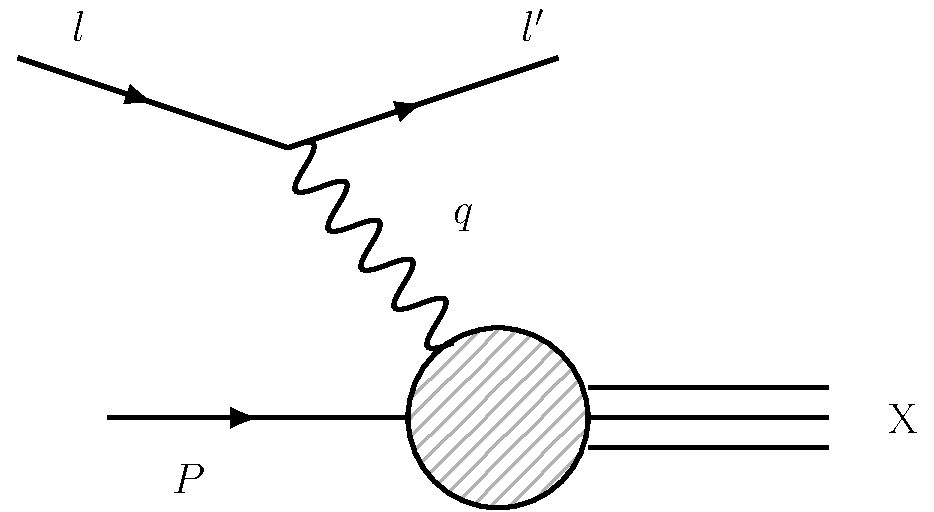
\includegraphics[scale=0.4]{Figures/DIS.pdf}
    \caption{Kinematics of deep inelastic electron--proton scattering}
    \label{fig:Deep Inelastic Scattering}
\end{figure}
\medskip

\subsection*{Kinematics}
We consider the scattering of a high energy electron off a proton target, via the exchange of a virtual photon (see \cref{fig:Deep Inelastic Scattering}). The full treatment would involve weak interactions, but for our purposes we only consider the electromagnetic interaction. We lable the incoming and outgoing electron momenta with $l^{\mu}$ and $l'^{\mu}$ respectively, the momentum of the proton by $P^{\mu}$ and the momentum transfer by the photon $q^{\mu}=l^{\mu}-l'^{\mu}$. We will assume that the mass of the electron and the proton constituents are negligible compared to the scale of the process. The centre-of-mass energy squared is then
\begin{align}
    s=(P+l)^{2}=m_{p}^{2}+2P\cdot l\,,
\end{align}
where $m_{p}$ is the mass of the proton. It follows that the momentum transfer squared is given by
\begin{align}
    q^{2}=2E_{l}E_{l'}(\cos\theta_{ll'}-1)\leq 0\,.
\end{align}
Therefore, it is useful to instead define $Q^{2}\equiv-q^{2}\geq 0$. The invariant mass of the final state $X$ is given by
\begin{align}
    m_{X}^{2}=(P+q)^{2}=m_{p}^{2}+2P\cdot q-Q^{2}\,.
\end{align}
In order to have \emph{deep} and \emph{inelastic} scattering, we must have the requirement that $Q^{2}\gg m_{p}^{2}$---\,the momentum transfer is so large that the proton target is very much excited\,---\,and inelastically $m_{X}^{2}\gg m_{p}^{2}$. 

The two independent Lorentz invariants for the hadron system are $Q^{2}$ and $P\cdot q$, but it is convenient to define additional invariant variables
\begin{align}
    x_{B}&=\frac{Q^{2}}{2P\cdot q}\,,\label{eq:Bjorken-x}
    \\
    y&=\frac{P\cdot q}{P\cdot l}=\frac{Q^{2}}{x_{B}(s-m_{p}^{2})}\,.
\end{align}
Here $x_{B}$ is called \emph{Bjorken-x}, which we from now will only denote by $x$. Kinematically $x$ is restricted to the range $Q^{2}/s+Q^{2}\leq x \leq 1$, neglecting terms of $\mathcal{O}(m_{p}^{2}/Q^{2})$. In the parton model we will find that $x$ gives an estimate for the hadron's momentum fraction that is carried by the struck parton. In the rest frame of the proton $y$ is the fractional energy loss of the electron, but it is not an independent variable since it is given by $Q^{2}$ and $x$.



\subsection*{Factorization and Bjorken Scaling}
From the above picture, the parton model describes DIS without the strong interaction participating, as all strong effects have been absorbed into the proton. Consequently, the proton is like a black box, where we have no idea of its structure, except that we can extract a parton from it.

Before we write down the amplitude and differential cross-section for this process, we must define some relations for current matrix elements. A fermion current is $j^{\mu}(z)=\bar{\psi}(z)\gamma^{\mu}\psi(z)$, with $\psi(z)$ the fermion field. A generic current matrix element for a fermion is then given by
\begin{align}\label{eq:generic current matrix element}
    \bra{k'}j^{\mu}(z)\ket{k}=\Bar{u}(k')\gamma^{\mu}u(k)\,e^{i(k'-k)\cdot z}\,,
\end{align}
where we used $z$ as space-time variable in order to avoid confusion with the Bjorken-$x$. The relation in \cref{eq:generic current matrix element} can be derived using the expansion of the fermion fields in terms of creation and annihilation operators. Thus, a shorthand for the spinor product $\Bar{u}(k')\gamma^{\mu}u(k)$ coming out of matrix elements is just the current matrix element at space-time point $z=0$, i.e. 
\begin{align}
    \bra{k'}j^{\mu}(0)\ket{k}=\Bar{u}(k')\gamma^{\mu}u(k)\,.
\end{align}
Then we can write the amplitude for DIS as
\begin{align}
    \mathcal{M}=\bra{l'}\,j_{L}^{\mu}\,\ket{l}\bra{X}\,j_{H}^{\nu}\,\ket{P}\,D_{\mu\nu}(q)\,,
\end{align}
where $D_{\mu\nu}(q)$ is just the regular photon propagator, see \cref{eq:photon propagator without gauge choice}. The differential cross section then takes the form
\begin{align}
    d\sigma&=\frac{1}{4\,P\cdot l}\frac{d^{3}l'}{(2\pi)^{3}\,2E_{l'}}\sum_{X}\int\frac{d^{3}p_{X}}{(2\pi)^{3}\,2E_{X}}(2\pi)^{4}\delta^{(4)}(P+l-p_{X}-l)|\mathcal{M}|^{2}\nonumber\,,
\end{align}
giving
\begin{align}\label{eq:DIS differential cross section}
    E_{l'}\frac{d\sigma}{d^{3}l'}&=\frac{2}{s-m_{p}^{2}}\frac{\alpha^{2}}{Q^{4}}L_{\mu\nu}W^{\mu\nu}\,,
\end{align}
where $\alpha$ is the fine structure constant. As we only consider photon exchange, the lepton tensor is completely determined by QED
\begin{align}
    L_{\mu\nu}=\frac{1}{2}\text{tr}[\slashed{l'}\gamma_{\mu}\slashed{l}\gamma_{\nu}]=2\big(l_{\mu}l'_{\nu}+l_{\nu}l'_{\mu}-g_{\mu\nu}l\cdot l'\big)\,.
\end{align}
In contrast, the hadronic tensor contains all the information about the interaction between the electromagnetic current $j_{H}^{\mu}$ and the proton $P$
\begin{align}
    W^{\mu\nu}&=4\pi^{3}\sum_{X}\int\frac{d^{3}p_{X}}{(2\pi)^{3}\,2E_{X}}\delta^{(4)}(P+q-p_{X})\,\bra{P}\,j^{\dag\,\mu}(0)\,\ket{X}\bra{X}\,j^{\nu}(0)\,\ket{P}\nonumber
    \\
    &=\frac{1}{4\pi}\int d^{4}z\,\sum_{X}\int\frac{d^{3}p_{X}}{(2\pi)^{3}\,2E_{X}}\,e^{iz\cdot(P+q-p_{X})}\,\bra{P}\,j^{\dagger\,\mu}(0)\,\ket{X}\bra{X}\,j^{\nu}(0)\,\ket{P}\,,\nonumber
\end{align}
where we used the integral representation of the four dimensional delta function. Further, we can use the translation operator
\begin{align}\label{eq:translation operator}
    \,\bra{P}\,j^{\dagger\,\mu}(0)\,\ket{X}e^{iz\cdot(P-p_{X})}&=\,\bra{P}e^{iz\cdot\hat{P}}\,j^{\dagger\,\mu}(0)\,e^{-iz\cdot\hat{P}}\ket{X}\nonumber
    \\
    &=\bra{P}\,j^{\dagger\,\mu}(z)\,\ket{X}\,,
\end{align}
and integrate out a complete set of states by the use of the completeness relation:
\begin{align}\label{eq:complete set of states}
    \sum_{X}\int\frac{d^{3}p_{X}}{(2\pi)^{3}\,2E_{X}}\ket{X}\bra{X}=\boldsymbol{1}\,.
\end{align}
The hadronic tensor can then be written as
\begin{align}\label{eq:hadronic tensor in terms of currents}
    W^{\mu\nu}=\frac{1}{4\pi}\int d^{4}z\,e^{iq\cdot z}\bra{P}\,j^{\dagger\,\mu}(z)j^{\nu}(0)\ket{P}\,.
\end{align}

This tensor can now be decomposed in terms of tensors that governs the kinematics times scalar functions. To do this, we use that the electromagnetic current is conserved, $\partial_{\mu}j^{\mu}=0$, so that the hadronic tensor satisfies the Ward identity $q_{\mu}W^{\mu\nu}=0$. Further, using that the strong interaction is parity invariant and $W^{\mu\nu}$ is hermitian, the most general form of the hadronic tensor for unpolarized protons can be written as
\begin{align}\label{eq:1stparametrized hadronic tensor}
    W^{\mu\nu}=\Big(-g^{\mu\nu}+\frac{q^{\mu}q^{\nu}}{q^{2}}\Big)F_{1}(x,Q^{2})+\Big(P^{\mu}+\frac{1}{2x}q^{\mu}\Big)\Big(P^{\nu}+\frac{1}{2x}q^{\nu}\Big)\frac{1}{P\cdot q}F_{2}(x,Q^{2})\,.
\end{align}
The scalar functions $F_{1}$ and $F_{2}$ are the structure functions we alluded to earlier. They contain the information of the hadron structure as \textquote{seen} by the virtual photon. Combining this with the leptonic tensor we find that
\begin{align}
    L_{\mu\nu}W^{\mu\nu}=\frac{2Q^{2}}{xy^{2}}\Big[\Big(1-y+\frac{y^{2}}{2}\Big)2xF_{1}(x,Q^{2})+(1-y)\big(F_{2}(x,Q^{2})-2xF_{1}(x,Q^{2})\big)\Big]\,.
\end{align}
Plugging this into \cref{eq:DIS differential cross section}, and neglecting terms of $\mathcal{O}( m_{p}^{2}/Q^{2})$ gives the unpolarized electron--proton DIS cross section
\begin{align}\label{eq:full differential DIS}
    \frac{d^{2}\sigma}{dxdy}=\frac{4\pi\alpha^{2}s}{Q^{4}}\Big[\Big(1-y+\frac{y^{2}}{2}\Big)2xF_{1}(x,Q^{2})+(1-y)\big(F_{2}(x,Q^{2})-2xF_{1}(x,Q^{2})\big)\Big]\,.
\end{align}
To find a parton model prediction for the behaviour of the structure functions, we calculate the partonic equivalent of $\cref{eq:full differential DIS}$. Thus, we are only interested in electron--quark scattering, $e^{-}(l)q(p)\rightarrow e^{-}(l')q(p')$. By using the Mandelstam variables
\begin{align}
    \hat{s}=(l+p)^{2}\,,\hspace{0.5cm}\hat{t}=(l-l')\,,\hspace{0.5cm}\hat{u}=(p-l')\,,
\end{align}
it is straightforward to show that the spin/colour averaged amplitude takes the form
\begin{align}
    \langle\, |\mathcal{M}|^{2}\rangle = 2Q_{q}^{2}e^{4}\,\frac{\hat{s}^{2}+\hat{u}^{2}}{\hat{t}^{2}}\,,
\end{align}
where $Q_{q}$ is the fractional charge of the quark. Using the standard result for the differential cross section for massless $2\rightarrow 2$ scattering:
\begin{align}
    \frac{d\hat{\sigma}}{d\hat{t}}=\frac{1}{16\pi\hat{s}^{2}} \langle\, |\mathcal{M}|^{2}\rangle\,,
\end{align}
which after some rewriting will give the partonic differential cross section
\begin{align}
    \frac{d\hat{\sigma}}{dy}=Q_{q}^{2}\frac{4\pi\alpha^{2}\hat{s}}{Q^{4}}\Big(1-y+\frac{y^{2}}{2}\Big)\,.
\end{align}
In order to relate the hard cross section with the full cross section, we define the quark momentum as a fraction of the proton momentum,
\begin{align}
    p^{\mu}=\xi P^{\mu}\,, \hspace{0.8cm}0<\xi<1\,,
\end{align}
such that $\hat{s}=\xi s$. If we approximate with an on-shell constraint for the outgoing quark, we find that 
\begin{align}
    p'^{2}=(p+q)^{2}=2\xi P\cdot q -Q^{2}=0\,,
\end{align}
implying that $\xi=x$. The on-shell constraint fixes the momentum fraction to equal the Bjorken variable, but this is of course not a general result. The Bjorken-$x$ is a kinematical constraint defining the process, while $\xi$ is just a momentum fraction that is independent of the process. To obtain a double differential cross-section as in \cref{eq:full differential DIS}, we simply use that 
\begin{align}
    \int_{0}^{1}dx\,\delta(x-\xi)=1\,,
\end{align}
and write
\begin{align}\label{eq:partonic differential DIS}
    \frac{d^{3}\hat{\sigma}}{dxdyd\xi}=Q_{q}^{2}\frac{4\pi\alpha^{2}s}{Q^{4}}\Big(1-y+\frac{y^{2}}{2}\Big)\,\xi\,\delta(x-\xi)\,.
\end{align}
We can now use the parton model interpretation of $f_{q}(\xi)$ as a probability and convolute it with the partonic part. To find the electron--proton differential cross section we simply integrate over all possible fraction $\xi$ and sum over quark flavour
\begin{align}\label{eq:parton model factorization}
    \frac{d^{2}\sigma}{dxdy}&=\sum_{q}\int_{0}^{1}d\xi\,f_{q}(\xi)\,\frac{d^{3}\hat{\sigma}}{dxdyd\xi}\nonumber
    \\
    &=\frac{4\pi\alpha^{2}s}{Q^{4}}\Big(1-y+\frac{y^{2}}{2}\Big)\,\sum_{q}Q_{q}^{2}\,x\,f_{q}(x)\,.
\end{align}
Then if we compare \cref{eq:parton model factorization} with \cref{eq:full differential DIS} we see that the proton structure functions in this simple model is given by
\begin{align}\label{eq:proton structure functions F_2 and F_1}
    F_{2}(x)=2xF_{1}(x)&=\sum_{q}Q_{q}^{2}\,x\,f_{q}(x)\,.
\end{align}
This result shows that in the regime where $Q^{2}$ is very large, we have that the structure functions only depend on the Bjorken-$x$. This is what is called \emph{Bjorken scaling}, and the result $F_{2}=2xF_{1}$ is known as the \emph{Callan-Gross relation}. The Callan-Gross relation follows from the spin-$1/2$ nature of quarks and was later confirmed by structure function measurements. These predictions made the parton model an intriguing model to further explore the structure of hadrons.

In \cref{eq:parton model factorization} we convoluted the partonic cross section with the parton distributions resulting in a hadronic cross section. Therefore, we can also define quark structure functions that we can convolute with the parton distribution, giving the proton structure functions. We see that if we define
\begin{align}
    \hat{F}_{2}=Q_{q}^{2}\,x\,\delta(1-x)\,,\label{eq:quark structure function hat_F2}
    \\
    \hat{F}_{1}=\frac{1}{2}Q_{q}^{2}\,\delta(1-x)\,,\label{eq:quark structure function hat_F1}
\end{align}
we can write the parton model factorization formulas for the proton structure functions as,
\begin{align}
    F_{2}(x)&=\sum_{q}\int_{x}^{1}d\xi\,f_{q}(\xi)\hat{F}_{2}\Big(\frac{x}{\xi}\Big)=\sum_{q}Q_{q}^{2}\,x\,f_{q}(x)\label{eq:collinear factorization parton model F_2}\,,
    \\
    F_{1}(x)&=\sum_{q}\int_{x}^{1}\frac{d\xi}{\xi}f_{q}(\xi)\hat{F}_{1}\Big(\frac{x}{\xi}\Big)=\frac{1}{2}\sum_{q}Q_{q}^{2}f_{q}(x)\label{eq:collinear factorization parton model F_1}\,,
\end{align}
giving the same result as above. The integration bound follows from $x/\xi\leq 1$. In the same manner the differential cross section can be written in the following way:
\begin{align}
     d\sigma(x,Q^{2})&=\sum_{q}\int_{x}^{1}d\xi\,f_{q}(\xi)\,d\hat{\sigma}\Big(\frac{x}{\xi},Q^{2}\Big)\,,
    \\
\end{align}
which is known as \emph{collinear factorization} of DIS in the parton model. An important point to make is that the above factorized integrals are convolutions defined in \emph{Mellin Space}, see \cref{sec:Appendix Mellin Transform}. Mellin transformations and their properties are very useful in studying QCD, which we will lay out in more detail in \cref{chap:Resummation in QCD}.

The collinear terminology used here refers to the fact that we have only considered the case where the quark momentum is in the same direction as the proton. We should, therefore, point out that $f_{q}(\xi)$ is formally defined as
\begin{align}
    f_{q}(\xi)=\int d^{2}k_{\perp}f_{q}(\xi,k_{\perp})\,,
\end{align}
where the transverse momentum dependence has been integrated out. It should also be pointed out that this is only valid as we only measure the final state lepton. If we wanted to take into account the final state hadrons we would have to use \emph{transverse momentum distributions} (TMDs), which is much more complicated. In this chapter we will only consider processes, like DIS and Drell-Yan, where the final state hadrons are integrated out.

\medskip
We have seen that the parton model result can give predictions that have been confirmed by experiments, but it is a phenomenological model and is not a formal treatment of the strong interaction. However, the concept of factorization is exactly what makes one take a field theoretical approach to hadronic scattering processes. Including QCD into the parton model results in interactions between the partons, and the assumption of free partons does not hold anymore. Therefore, the above factorization formulas are invalid and we must make a more precise definition of factorization in QCD. To this end, we will consider the case of QCD corrections to the DIS process in the next section. 

\medskip
To end this section we will make a brief remark about the difference between structure functions and parton distribution functions. The structure functions appeared when we parametrized the hadronic tensor, which is process dependent. That is, if we considered DIS neutrino scattering, the structure functions would change as we, in that case, considered $W$ or $Z$ boson exchange. The main idea behind factorization is that, inside the structure functions, we can factorize out the proton content from the process dependent part. The factorization ansatz in \cref{eq:parton model factorization} is required to be valid for any process, meaning that the PDFs are universal. Thus, the PDFs can be extracted from DIS electron--proton scattering experiments and re-used in another experiment like DIS neutrino--proton scattering and proton--proton collisions at the LHC.

%%%%%%%%%%%%%%%%%%%%%%%%%%%%%%%%%%%%%%%%%
\subsection{Collinear Factorization in QCD}\label{sec:QCD and Collinear factorization}
In \cref{sec:DIS and Parton model} we saw that the observables in the parton model could be written on a factorized form. The crucial element of that result is the assumption that the quark momentum is a fraction of the proton's momentum, $p^{\mu}=\xi P^{\mu}$. This is in general not true, as the quark will also have transverse components. To highlight the validity of the parton model assumption it is useful to use \emph{light-cone coordinates}, see \cref{sec:Appendix Light-cone coordinates}. 

By considering the case where the proton has no transverse momentum components, the general form of the proton and parton momenta can be parametrized as
\begin{align}
    P^{\mu}=\Big(P^{+},\frac{m_{p}^{2}}{2P^{+}},0_{\perp}\Big)\,,\hspace{1cm}
    p^{\mu}=(p^{+},p^{-},p_{\perp})\,.
\end{align}
It is safe to assume that in the protons rest frame, the distribution of partons is isotropic, and that the components of the parton momentum is of the order of the proton mass. We are free to choose frame, so by choosing the frame where $P^{+}\rightarrow \infty$, the only remaining component of the proton momentum is its plus-component. It is also hard to imagine that the partons will not follow the proton along this direction---at least if we assume no gluon radiation---so we find that
\begin{align}
    P^{\mu}=(P^{+},0^{-},0_{\perp})\,,\hspace{1cm}
    p^{\mu}\approx(p^{+},0^{-},0_{\perp})\,.
\end{align}
This is what is called the \emph{infinite momentum frame} (IMF), and the partons transverse components has been neglected compared to the plus-component, $p^{+}\gg p_{\perp}\sim m_{p}$. We can now assume that the struck quark has a fraction $\xi$ of the proton's momentum, giving that in the infinite momentum frame the parton momentum is fully collinear to the proton momentum
\begin{align}
    p^{\mu}=\xi P^{\mu}\,,
\end{align}
which is the result we used for the parton model in \cref{sec:DIS and Parton model}. 

However, if the struck parton is a quark that has just emitted a gluon this is no longer necessarily true, and we will need a more general parametrization of the momenta. We can use $p^{+}=\xi P^{+}$ to parametrize the parton momentum in terms of the large plus-component $P^{+}$
\begin{align}\label{eq:light-cone parametrization}
    P^{\mu}=\Big(P^{+},\frac{m_{p}^{2}}{2P^{+}},0_{\perp}\Big)\,,\hspace{1cm}p^{\mu}=\Big(\xi P^{+},\frac{p^{2}+p_{\perp}^{2}}{2\xi P^{+}},p_{\perp}\Big)\,,
\end{align}
which reproduces the infinite momentum frame limit for $p^{2},p_{\perp}^{2},m_{p}^{2}\ll P^{+}$. In turn the photon momentum can be parametrized as
\begin{align}\label{eq:light-cone photon momenta}
    q^{\mu}=\Big(0,\frac{Q^{2}}{2xP^{+}},q_{\perp}\Big)\,,
\end{align}
where $-q^{2}=q_{\perp}^{2}=Q^{2}$ and $P\cdot q=Q^{2}/2x$, meaning that this choice reproduces the known kinematics in DIS, given in \cref{eq:Bjorken-x}. Not only does light-cone coordinates formalise the parton model assumption of fully collinear partons in the IMF, but as we will later see it is in this formalism that the parton model has it's closest relation to field theory. In the following calculations we will parametrize all momenta as in \cref{eq:light-cone parametrization}.

\medskip
In the parton model calculation we found that the structure functions scale, i.e. $F(x,Q^{2})\rightarrow F(x)$ in the Bjorken limit $Q^{2}\rightarrow \infty$. By including QCD into this picture, $F(x,Q^{2})$ will have terms that are proportional to $\ln{Q^{2}}$, i.e. we have logarithmic breaking of Bjorken scaling. The key point is that the original quark can emit a gluon before being struck by the photon and will acquire a transverse component that can not be neglected. As we shall see below, when integrating over the intermediate quark momentum, the integral over this transverse component extends up to the kinematic limit  $Q^{2}$, leading to this logarithmic dependancy of $Q^{2}$. 

Factorization in QCD is therefore the determination of at which point the emitted gluon belongs to the soft part or the hard part of the scattering. The correct way to determine this\,---\,at least in the collinear case\,---is to define a separation in terms of an energy scale $\mu_{F}$ (factorization scale). Thus, if the gluon is emitted at a scale lower than $\mu_{F}$ it is part of the PDF (soft part) and if it is emitted at a scale larger than $\mu_F$ it is part of the partonic process (hard part). The all order proof of factorization in QCD is beyond the scope of this thesis, so here we will investigate the $\mathcal{O}(\alpha_s)$ correction to DIS and see how that changes the parton model factorization.

\medskip
\subsection*{One gluon emission}
\begin{figure}
    \centering
    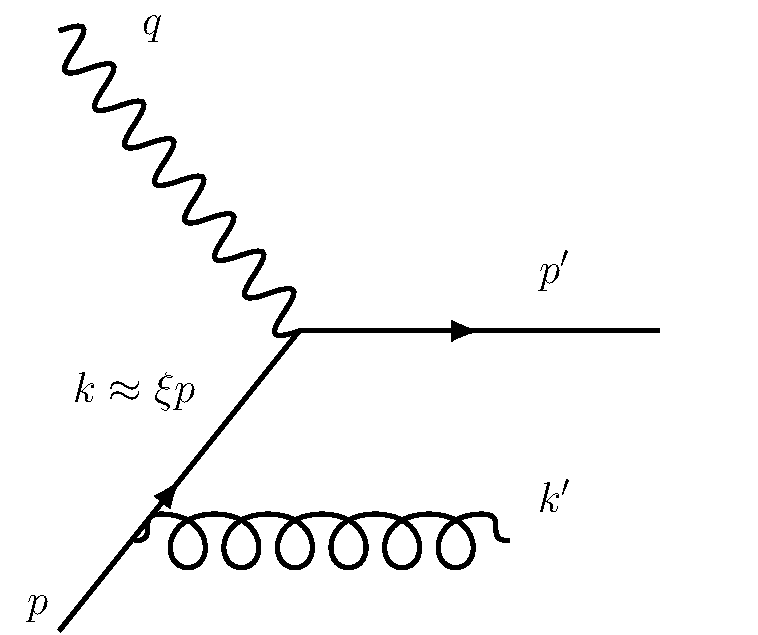
\includegraphics[scale=0.4]{Figures/gluonemissionDIS.pdf}
    \caption{Gluon emission from initial quark.}
    \label{fig:DISgluonemission}
\end{figure}

At NLO there are two real gluon diagrams and three virtual gluon diagrams in DIS. The real diagrams are emission from initial and final quark line, while the virtual diagrams are self energy diagrams of the initial and final state together with exchange of a gluon between the initial and final quark lines.
However, we will only consider gluon emission from the initial quark line, given in \cref{fig:DISgluonemission}. The reason for this is that we will choose to work with gluons in light-cone gauge, and in this gauge this is the only diagram that gives a logarithmic divergence. The other diagrams will give finite results that are unimportant for the current discussion and will be omitted for brevity.

\medskip
The way to proceed is to investigate corrections to the hadronic tensor and extract the structure functions from it. The proton strucure functions were in the parton model written as a convolution between the PDF and the quark structure functions, see \cref{eq:collinear factorization parton model F_2} and \cref{eq:collinear factorization parton model F_1}. The hadronic tensor can also be written on this convoluted form
\begin{align}
    W^{\mu\nu}(x,Q^{2})=\sum_{q}\int_{x}^{1}\frac{d\xi}{\xi}f_{q}(\xi)\hat{W}^{\mu\nu}\Big(\frac{x}{\xi},Q^{2}\Big)\,,
\end{align}
where $\hat{W}^{\mu\nu}$ refers to the partonic part that are calculable in perturbation theory. Thus, we will calculate $\hat{W}^{\mu\nu}$ up to $\mathcal{O}(\alpha_s)$ and extract $\hat{F}_{2}$ from it, enabling us to compare with \cref{eq:collinear factorization parton model F_2} to see the effect it has on the PDF.

In \cref{eq:1stparametrized hadronic tensor} we parametrized the hadronic tensor as
\begin{align}
    W^{\mu\nu}=\Big(-g^{\mu\nu}+\frac{q^{\mu}q^{\nu}}{q^{2}}\Big)F_{1}(x,Q^{2})+\Big(P^{\mu}+\frac{1}{2x}q^{\mu}\Big)\Big(P^{\nu}+\frac{1}{2x}q^{\nu}\Big)\frac{1}{P\cdot q}F_{2}(x,Q^{2})\,.
\end{align}
However, in higher order calculations there is an alternative parametrization that comes in handy when we want to extract the structure functions. Hence, we define normalized basis vectors (factors and terms $\mathcal{O}(m_{p}^{2}/Q^{2})$ are as usual neglected)
\begin{align}\label{eq:basis vectors}
    \hat{q}^{\mu}&\equiv\frac{q^{\mu}}{Q}\, ,\hspace{1cm}\hat{t}^{\mu}\equiv\frac{1}{Q}(q^{\mu}+2xP^{\mu})\,.
\end{align}
These basis vector satisfy: $\hat{q}\cdot\hat{t}=0$, $\hat{q}^{2}=-1$ and $\hat{t}^{2}=1$, meaning that $\hat{q}$ is spacelike and $\hat{t}$ is timelike. With respect to these basis vectors one can also define a transverse tensor
\begin{align}
    g_{\perp}^{\mu\nu}\equiv g^{\mu\nu}+\hat{q}^{\mu}\hat{q}^{\nu}-\hat{t}^{\mu}\hat{t}^{\nu}\,,
\end{align}
from which the following relations follow
\begin{align}
    \hat{t}_{\mu}g_{\perp}^{\mu\nu}&=0
    \\
    \hat{q}_{\mu}g_{\perp}^{\mu\nu}&=0
    \\
    g_{\perp}^{\mu\nu}g_{\perp\,\mu\nu}&=2\,,
\end{align}
making it consistent with \cref{eq:trasnversal tensor}. With these definitions it is straightforward to rewrite the hadronic tensor as
\begin{align}\label{eq:2ndparametrized hadronic tensor}
    W^{\mu\nu}(x,Q^{2})=-g_{\perp}^{\mu\nu}F_{1}(x,Q^{2})+\frac{\hat{t}^{\mu}\hat{t}^{\nu}}{2x}\big(F_{2}(x,Q^{2})-2xF_{1}(x,Q^{2})\big)\,,
\end{align}
from which the structure functions can be extracted by applying appropriate tensors on the hadronic tensor
\begin{align}
    F_{1}&=-\frac{1}{2}g_{\perp}^{\mu\nu}W_{\mu\nu}\,,\label{eq:extracting F_1}
    \\
    F_{2}&=x(2\hat{t}^{\mu}\hat{t}^{\nu}-g_{\perp}^{\mu\nu})W_{\mu\nu}\,.\label{eq:extracting F_2}
\end{align}
For the $F_{2}$ projection is is useful to note that $(2\hat{t}^{\mu}\hat{t}^{\nu}-g_{\perp}^{\mu\nu})g_{\mu\nu}=0$, which will cancel all terms involving $g^{\mu\nu}$ in the Dirac traces. 

The amplitude for the gluon emission in \cref{fig:DISgluonemission}, is given by
\begin{align}
    \mathcal{M}^{\mu}=-igQ_{q}t^{a}\varepsilon_{\beta}^{*}(k')\,\bar{u}(p')\,\gamma^{\mu}\frac{\slashed{k}}{k^{2}}\gamma^{\beta}\,u(p)\,.
\end{align}
We average over incoming spin and colour, sum over final spin, colour and gluon polarization,
\begin{align}
    \langle\,|\mathcal{M}|^{2}\rangle^{\mu\nu}&=\frac{1}{N_{s}N_{c}}\sum_{a,b}\sum_{\text{spin}}\sum_{\text{pol}}\big(|\mathcal{M}|^{2}\big)^{\mu\nu}\,\nonumber
    \\
    &=\frac{C_{F}}{N_s}Q_{q}^{2}g^{2}\frac{1}{k^{4}}\sum_{\text{pol}}\varepsilon_{\alpha}(k')\varepsilon_{\beta}^{*}(k')\,\text{tr}[\gamma^{\nu}\slashed{p}'\gamma^{\mu}\slashed{k}\gamma^{\alpha}\slashed{p}\gamma^{\beta}\slashed{k}]\,.
\end{align}
We can then use the gluon polarization sum in the light-cone gauge (see \cref{eq:gluon polarization sum light-cone gauge})
\begin{align}
    \sum_{\text{pol}}\varepsilon_{\alpha}(k')\varepsilon_{\beta}^{*}(k')&=-g_{\alpha\beta}+\frac{k'_{\alpha}\,n_{-\,\beta}}{k'^{+}}+\frac{k'_{\beta}\,n_{-\,\alpha}}{k'^{+}}\,,
\end{align}
which will give the following expression for the Dirac trace
\begin{align}
    \sum_{\text{pol}}\varepsilon_{\alpha}(k')\varepsilon_{\beta}^{*}(k')\,\text{tr}[\gamma^{\nu}\slashed{p}'\gamma^{\mu}\slashed{k}\gamma^{\alpha}\slashed{p}\gamma^{\beta}\slashed{k}]=&-\text{tr}[\gamma^{\nu}\slashed{p}'\gamma^{\mu}\slashed{k}\gamma^{\alpha}\slashed{p}\gamma_{\alpha}\slashed{k}]+\frac{1}{k'^{+}}\text{tr}[\gamma^{\nu}\slashed{p}'\gamma^{\mu}\slashed{k}\slashed{k}'\slashed{p}\gamma^{+}\slashed{k}]\nonumber
    \\
    &+\frac{1}{k'^{+}}\text{tr}[\gamma^{\nu}\slashed{p}'\gamma^{\mu}\slashed{k}\gamma^{+}\slashed{p}\slashed{k}'\slashed{k}]\,.\nonumber
\end{align}

These traces can be calculated using the relations given in \cref{sec:Appendix Dirac gamma matrices}, but it is tedious so we will just write out the main steps. The first trace can be simplified to
\begin{align}
    \text{tr}[\gamma^{\nu}\slashed{p}'\gamma^{\mu}\slashed{k}\gamma^{\alpha}\slashed{p}\gamma_{\alpha}\slashed{k}]=-4p\cdot k\,\text{tr}[\gamma^{\nu}\slashed{p}'\gamma^{\mu}\slashed{k}]+2k^{2}\,\text{tr}[\gamma^{\nu}\slashed{p}'\gamma^{\mu}\slashed{p}]\,,
\end{align}
and the last two traces can first be simplified by using that $k'=p-k$, giving
\begin{align}
    \text{tr}[\gamma^{\nu}\slashed{p}'\gamma^{\mu}\slashed{k}\slashed{k}'\slashed{p}\gamma^{+}\slashed{k}]&=-k^{2}\,\text{tr}[\gamma^{\nu}\slashed{p}'\gamma^{\mu}\slashed{p}\gamma^{+}\slashed{k}]\,,
    \\
    \text{tr}[\gamma^{\nu}\slashed{p}'\gamma^{\mu}\slashed{k}\gamma^{+}\slashed{p}\slashed{k}'\slashed{k}]&=-k^{2}\,\text{tr}[\gamma^{\nu}\slashed{p}'\gamma^{\mu}\slashed{k}\gamma^{+}\slashed{p}]\,,
\end{align}
where the sum of these two traces can be rewritten as
\begin{align}
    -k^{2}\text{tr}[\gamma^{\nu}\slashed{p}'\gamma^{\mu}(\slashed{k}+\slashed{p})\gamma^{+}(\slashed{p}+\slashed{k})]=&-2(k^{+}+p^{+})k^{2}\,\text{tr}[\gamma^{\nu}\slashed{p}'\gamma^{\mu}\slashed{k}]\nonumber
    \\
    &-2(k^{+}+p^{+})k^{2}\,\text{tr}[\gamma^{\nu}\slashed{p}'\gamma^{\mu}\slashed{p}]\nonumber
    \\
    &+k^{2}(k^{2}+2p\cdot k)\text{tr}[\gamma^{\nu}\slashed{p}'\gamma^{\mu}\gamma^{+}]\,.\nonumber
\end{align}
Collecting all terms and using the cyclic property of the trace, we find that the sum of all traces can be written as
\begin{align}
    \sum\text{tr}(...)=&\,\Big(4p\cdot k-2k^{2}\frac{k^{+}+p^{+}}{k^{+}-p^{+}}\Big)\text{tr}[\slashed{k}\gamma^{\mu}\slashed{p}'\gamma^{\nu}]\nonumber
    \\
    &-2k^{2}\Big(1+\frac{k^{+}+p^{+}}{k^{+}-p^{+}}\Big)\text{tr}[\slashed{p}\gamma^{\mu}\slashed{p}'\gamma^{\nu}]\nonumber
    \\
    &+\frac{k^{2}}{k^{+}-p^{+}}\big(k^{2}+2p\cdot k\big)\text{tr}[\slashed{n}_{-}\gamma^{\mu}\slashed{p}'\gamma^{\nu}]\,,\nonumber
\end{align}
where we used that $\gamma^{+}=\slashed{n}_{-}$, such that all the traces take the same form. For generic vectors, $a^{\mu}$ and $b^{\mu}$, these traces evaluate to\footnote{See \cref{sec:Appendix Dirac gamma matrices} for more detail on traces.}
\begin{align}\label{eq:tracetrace}
    \text{tr}[\slashed{a}\gamma^{\mu}\slashed{b}\gamma^{\nu}]=4(a^{\mu}b^{\nu}+a^{\nu}b^{\mu}-g^{\mu\nu}a\cdot b)\,.
\end{align}
Hence, we write the averaged amplitude as
\begin{align}\label{eq:ththehte amp}
    \langle\,|\mathcal{M}|^{2}\rangle^{\mu\nu}=\frac{C_{F}}{N_s}Q_{q}^{2}g^{2}\frac{1}{k^{4}}\sum\text{tr}(...)\,.
\end{align}


To calculate $\hat{W}^{\mu\nu}$, we must integrate over the final state particles, giving
\begin{align}
    \hat{W}^{\mu\nu}=\frac{1}{4\pi}\int d\mathcal{P}_{2}\,\langle\, |\mathcal{M}|^{2}\rangle \,,
\end{align}
where $4\pi$ comes from the normalization in \cref{eq:hadronic tensor in terms of currents}. The n-body phase space for on-shell massless particles is given by \cref{eq:n-body phase space}, so the two-body phase space takes the form
\begin{align}\label{eq:DIS differential phase space}
    d\mathcal{P}_{2}&=\int\frac{d^{4}k'}{(2\pi)^{3}}\frac{d^{4}p'}{(2\pi)^{3}}\,\delta^{+}(k'^{2})\delta^{+}(p'^{2})(2\pi)^{4}\delta^{(4)}(p+q-k'-p')\nonumber
    \\
    &=\frac{1}{4\pi^{2}}\int d^{4}k\,\delta^{+}\big((p-k)^{2}\big)\delta^{+}\big((k+q)^{2}\big)\,,
\end{align}
where we use that $\delta^{+}(k'^{2})\equiv \delta(k'^{2})\theta(k'^{+})$\footnote{In light-cone coordinates the usual Heaviside function $\theta(k^{0})$ is replaced by $\theta(k^{+})$.}.
Note that we work explicitly in four dimensions, which mean we will not use dimensional regularization in this calculation. For the Drell-Yan process (see \cref{sec:Drell-Yan Hadronic Cross Section}), we will perform a full calculation using dimensional regularization, but for physical intuition it is more useful to use momentum cutoff in DIS.  

\medskip
In the partonic system we assume that the original quark has no transverse components and move in the plus direction, the virtual\footnote{All quarks are kind of virtual, but this is common terminology in scattering processes to specify that it is intermediate, i.e. propagating and off-shell.} quark on the other hand may have large transverse components due to the radiation of a gluon from the original quark. Thus, the relevant momenta in the partonic system is given by:
\begin{align}
    p^{\mu}&=(p^{+},0^{-},0_{\perp})\,,
    \\
    k^{\mu}&=\Big(\xi p^{+},\frac{k_{\perp}^{2}-|k^{2}|}{2\xi p^{+}},k_{\perp}\Big)\,,
    \\
    q^{\mu}&=\Big(0,\frac{Q^{2}}{2xp^{+}},q_{\perp}\Big)\,,
\end{align}
where we used that $k^{2}=-|k^{2}|$ because the intermediate quark is virtual. The arguments of the delta functions in \cref{eq:DIS differential phase space} is given by
\begin{align}
    (p-k)^{2}&=-2p\cdot k-|k^{2}|=-\frac{1}{\xi}\big(k_{\perp}^{2}-(1-\xi)|k^{2}|\big)\,,
    \\
    (k+q)^{2}&=2k\cdot q-|k^{2}|-Q^{2}=2P\cdot q\Big(\xi-x-\frac{|k^{2}|+2k_{\perp}\cdot q_{\perp}}{2P\cdot q}\Big)\,,
\end{align}
and the differential is given by
\begin{align}
    d^{4}k=dk^{+}dk^{-}d^{2}k_{\perp}=\frac{1}{4\xi}d\xi dk^{2}dk_{\perp}^{2}d\theta\,,
\end{align}
with $0<\theta<\pi$. Inserting these expression into \cref{eq:DIS differential phase space}, we get
\begin{align}
     d\mathcal{P}_{2}&=\frac{1}{(4\pi)^{2}P\cdot q}\int d\xi dk^{2}dk_{\perp}^{2}d\theta \hspace{2mm}\delta\big(k_{\perp}^{2}-(1-\xi)|k^{2}|\big)\,\delta\Big(\xi-x-\frac{|k^{2}|+2k_{\perp}\cdot q_{\perp}}{2P\cdot q}\Big)\,.
\end{align}

Now, there is no a priori reason why the transverse momentum (or equivalently $|k^{2}|$) should be small, but in the second delta function the effect of these are damped by $P\cdot q\sim Q^{2}$ so we proceed by neglecting this term. This again fixes $\xi=x$ in the final integration. We are actually jumping ahead here, but with a more thorough analysis it can be shown that this is in fact the case \cite{Ellis1996QCDAC}. The first delta function fixes $k_{\perp}^{2}=(1-\xi)|k^{2}|$, so we can just use it directly to rewrite the averaged amplitude in \cref{eq:ththehte amp}, giving
\begin{align}
    \langle\, |\mathcal{M}|^{2}\rangle^{\mu\nu}=&4\pi C_{F}\,Q_{q}^{2}\,\alpha_{s}\frac{1}{|k^{2}|}\Big[\frac{1}{\xi}\frac{1+\xi^{2}}{1-\xi}\big(8k^{(\mu}p'^{\nu)}-4g^{\mu\nu}k\cdot p'\big)\nonumber
    \\
    &+\frac{1}{1-\xi}\big(8p^{(\mu}p'^{\nu)}-4g^{\mu\nu}p\cdot p'\big) + \frac{1}{1-\xi}\frac{|k^{2}|}{p^{+}}\big(8n_{-}^{(\mu}p'^{\nu)}-4g^{\mu\nu}p'^{+}\big)\Big]\,.
\end{align}
where we have evaluated the traces using \cref{eq:tracetrace} and for notational simplicity defined $a^{(\mu}b^{\nu)}=(a^{\mu}b^{\nu}+a^{\nu}b^{\mu})/2$.

Let us then finally use \cref{eq:extracting F_2} to project out $\hat{F}_{2}$,
\begin{align}
    \hat{F}_{2}=\int d\mathcal{P}_{2}\,\,x(\hat{t}^{\mu}\hat{t}^{\nu}-g_{\perp}^{\mu\nu})\,\langle\, |\mathcal{M}|^{2}\rangle_{\mu\nu}\,.
\end{align}
In the following we will only list the divergent term as the finite ones are unimportant for this discussion. For the contraction with the matrix element we use that $p'=k+q$ and the basis vector $\hat{t}$ is found from \cref{eq:basis vectors}. Putting everything together is messy, but after the effect of the delta functions the divergent part takes the form\footnote{For a more detailed derivation of this term, see \cite{Ellis1996QCDAC}.}
\begin{align}\label{eq:divergent F_2}
    \hat{F}_{2}\,\big|_{\text{div}}=Q_{q}^{2}\frac{\alpha_s}{2\pi}\,xP_{q/q}(x)\int_{Q_{0}^{2}}^{Q^{2}}\frac{d|k^{2}|}{|k^{2}|}\,,
\end{align}
where the integral is regulated over $|k^{2}|$ in terms of a IR cut-off $Q_{0}^{2}$ and a UV cut-off $Q^{2}$, that follows from the kinematics. We have also defined a function $P_{q/q}(x)$, which is known as the \emph{quark--quark splitting function}
\begin{align}\label{eq:splitting function 1}
    P_{q/q}(x)=C_{F}\frac{1+x^{2}}{1-x}\,.
\end{align}
Its form is specific to the quark-quark-gluon vertex of QCD, and it represents the probability for a quark to split into another quark with momentum fraction $x$ and a gluon with momentum fraction $1-x$. Integrating \cref{eq:divergent F_2}, we find
\begin{align}\label{eq:divergent integrated F_2}
    \hat{F}_{2}\,\big|_{\text{div}}=Q_{q}^{2}\frac{\alpha_s}{2\pi}\,xP_{q/q}(x)\,\ln{\frac{Q^{2}}{Q_{0}^{2}}}\,.
\end{align}

If we include the leading order contribution given in \cref{eq:collinear factorization parton model F_2} and all finite terms, denoted $C_{q}(x)$, we have the quark structure function at $\mathcal{O}(\alpha_s)$
\begin{align}\label{eq:quark structure function correction}
    \hat{F}_{2}=Q_{q}^{2}\,x\Big(\delta(1-x)+\frac{\alpha_s}{2\pi}\big(P_{q/q}(x)\ln{\frac{Q^{2}}{Q_{0}^{2}}}+C_{q}(x)\big)\Big)\,.
\end{align}

The natural question that arises is how to interpret the divergence of the structure function. We observe that the singularity arises when the gluon is emitted fully collinear to the quark, i.e. $k_{\perp}=0$, and is therefore referred to as a \emph{collinear singularity}. To understand what is happening we need to realize that physically $k_{\perp}^{2}\rightarrow 0$ corresponds to a long-range part of the strong interaction which is not calculable in perturbation theory. Hence, if we use the PDFs to describe physics at long-range, we can convolute the structure function $\hat{F}_{2}$ with \textquote{bare} distributions $f_{q}^{0}$ to absorb the collinear singularity. This is a similar, but still different approach to the UV-renormalization procedure we discussed in \cref{sec:Renormalization}.

To get a clear understanding of how this is done we investigate the cut-off we made in \cref{eq:divergent F_2}. By imposing the IR cut-off we effectively integrate $k_{\perp}^{2}$ from $Q_{0}^{2}$ up to $Q^{2}$. Now, the kinematics of the process justifies the upper limit of $Q^{2}$ as $k_{\perp}$ is always smaller than or equal to $Q$\footnote{This follows from the fact that the transverse momentum of the gluon can not be larger than the scale of the process.}. However, in the IR-region there is no kinematical restriction on $k_{\perp}$. The lower cut-off ensures that the gluons with transverse momentum $k_{\perp}\leq Q_{0}$ is neglected from the hard part of the scattering. We can not drop these gluons entirely, so we absorb this part of the process into the PDF. We can then renormalize the PDF up to the arbitrary energy scale $\mu_F$.

\medskip
To obtain the proton structure function we convolute the quark structure function $\hat{F}_{2}$ of \cref{eq:quark structure function correction} with the bare PDF $f_{q}^{0}$ as we did for the parton model in \cref{eq:collinear factorization parton model F_2}, 
\begin{align}
    F_{2}(x,Q^{2})=\sum_{q}Q_{q}^{2}\,x\Big(f_{q}^{0}(x)+\frac{\alpha_s}{2\pi}\int_{x}^{1}\frac{d\xi}{\xi}f_{q}^{0}(\xi)\big[P_{q/q}\big(\frac{x}{\xi}\big)\ln{\frac{Q^{2}}{Q_{0}^{2}}}+C_{q}\big(\frac{x}{\xi}\big)\big]\Big)\,.
\end{align}
Then we can absorb the collinear singularities into the bare distribution at the factorization scale $\mu_F$, or in other words, we define a renormalized distribution
\begin{align}
    f_{q}(x,\mu_{F}^{2})=f_{q}^{0}(x)+\frac{\alpha_s}{2\pi}\int_{x}^{1}\frac{d\xi}{\xi}f_{q}^{0}(\xi)\big[P_{q/q}\big(\frac{x}{\xi}\big)\ln{\frac{\mu_{F}^{2}}{Q_{0}^{2}}}+C_{q}'\big(\frac{x}{\xi}\big)\big]\,,
\end{align}
which inserted into the expression for $F_{2}$ gives the finite result
\begin{align}\label{eq:renormalized F_2}
    F_{2}(x,Q^{2})=\sum_{q}Q_{q}^{2}\,x\int_{x}^{1}\frac{d\xi}{\xi}f_{q}(\xi,\mu_{F}^{2})\big[\delta\big(1-\frac{x}{\xi}\big)+\frac{\alpha_s}{2\pi}\Big(P_{q/q}\big(\frac{x}{\xi}\big)\ln{\frac{Q^{2}}{\mu_{F}^{2}}}+D_{q}\big(\frac{x}{\xi}\big)\Big)\big]\,.
\end{align}

This result says that we can choose an arbitrary energy scale $\mu_F$ to separate the process into two parts: a hard part where $k_{\perp}$ is larger than this scale, and a soft part where $k_{\perp}$ is smaller than this scale. Thus, we \textquote{hide} the divergence inside a part that were non-perturbative in the first place. We have alluded to this separation repeatedly and made this statement in the discussion of the parton model, but now we have extended that result to the correct framework of QCD. We also note that the only difference in QCD factorization and the parton model factorization is that the PDF and the hard part acquires a dependancy on the factorization scale. Although we have only demonstrated factorization to $\mathcal{O}(\alpha_S)$ in DIS, it has been proven to all orders in perturbation theory \cite{Collins:1989gx}. Another important feature of extending to QCD is that Bjorken-scaling is violated as $F_{2}$ is explicitly dependent on $Q^{2}$.

One important aspect of the renormalization procedure we have made here is that even though the factorization specifies a prescription of dealing with the logarithmic singularities, there is still an arbitrariness in the choice of the finite terms. In \cref{eq:renormalized F_2} we have that $D(x)=C(x)-C'(x)$, where $C'(x)$ is absorbed by the PDF and $D(x)$ is the terms that remains. However, we could have made another choice and absorbed all finite terms into the PDF, and the exact choice made is referred to as a \emph{factorization scheme}. The most common scheme is the $\overline{\text{MS}}$ scheme we mentioned in \cref{sec:Renormalization}, where the absorbed term is $C'=\ln 4\pi-\gamma_{E}$.

Due to the non-perturbative nature of long distance physics in QCD, the distributions $f_{q}(x,\mu_{F}^{2})$ are not directly   calculable from first principles, and must therefore be extracted from experiments or, more recently in lattice QCD. However, what can be calculated perturbatively is the dependence on the scale $\mu_{F}^{2}$. The proton structure function $F_{2}$ is an observable, meaning that it cannot depend on the choice of scale. This leads to the following requirement
\begin{align}
    \pdv{F_2}{\ln\mu_{F}^{2}}=0\,,
\end{align}
which leads to the following differential equation for the PDFs
\begin{align}\label{eq:1st evolution equation f_q}
    \pdv{}{\ln\mu_{F}^{2}}f_{q}(x,\mu_{F}^{2})=\frac{\alpha_{s}(\mu_{F}^{2})}{2\pi}\int_{x}^{1}\frac{d\xi}{\xi}P_{q/q}\big(\frac{x}{\xi}\big)\,f_{q}(\xi,\mu_{F}^{2})\,.
\end{align}
This evolution equation is similar to the $\beta$ function equation describing the evolution of the coupling $\alpha_{s}(\mu^{2})$, and is known as the Dokshitzer-Gribov-Altarelli-Parisi (DGLAP) equation. As it stands, this equation is only valid up to $\mathcal{O}(\alpha_s)$. To get an all order evolution equation we can expand the splitting function in the coupling,
\begin{align}
    P_{q/q}(x,\alpha_{s})=\sum_{n=0}^{\infty}\Big(\frac{\alpha_s}{2\pi}\Big)^{n+1}P_{q/q}^{(n)}(x)\,,
\end{align}
and write the evolution equation as
\begin{align}\label{eq:DGLAP equation}
    \pdv{}{\ln\mu_{F}^{2}}f_{q}(x,\mu_{F}^{2})=\int_{x}^{1}\frac{d\xi}{\xi}P_{q/q}\big(\frac{x}{\xi},\alpha_{s}(\mu_{F}^{2})\big)\,f_{q}(\xi,\mu_{F}^{2})\,,
\end{align}
where the higher order information is contained inside the splitting function. We can then identify the splitting function in \cref{eq:splitting function 1} and \cref{eq:1st evolution equation f_q} as the leading order splitting function $P_{q/q}^{(0)}$. For a more rigorous derivation of this generalization see \cite{Altarelli:1977zs}. 

In order to obtain a complete discussion of deep inelastic scattering in terms of parton distribution functions, there is one more ingredient that we have not considered. That is, we also need to consider the initial scattering of gluons. The $\mathcal{O}(\alpha_s)$ contribution for initial gluon scattering is through a t-channel boson-gluon fusion process. Following a similar line of argument as for the quark initial state this will lead to the gluon structure function
\begin{align}
    \hat{F}_{2}^{g}(x,Q^{2})=\sum_{q}Q_{q}^{2}\,x\,\frac{\alpha_s}{2\pi}\Big(P_{q/g}(x)\ln{\frac{Q^{2}}{Q_{0}^{2}}}+C_{g}(x)\Big)\,,
\end{align}
which is very similar to the quark structure function \cref{eq:quark structure function correction}, apart from the fact that at zeroth order in $\alpha_s$ there is no gluon radiation. The splitting function for this process is specific for the gluon-quark-quark vertex, and is given by
\begin{align}
    P_{q/g}(x)=\frac{1}{2}(x^{2}+(1-x)^{2})\,,
\end{align}
and is interpreted as the probability for a gluon to split into a quark with momentum fraction $x$ and another quark with momentum fraction $1-x$. 

As with the quark structure function we have to convolute the gluon structure function with a bare gluon distribution $f_{g}^{0}$, define a renormalized gluon distribution and add it to \cref{eq:renormalized F_2}. This is equivalent to redefining our renormalized quark parton distribution to also absorb the singular gluon term. Thus, we define
\begin{align}
    f_{q}(x,\mu_{F}^{2})=&f_{q}^{0}(x)+\frac{\alpha_s}{2\pi}\int_{x}^{1}\frac{d\xi}{\xi}f_{q}^{0}(\xi)\big[P_{q/q}\big(\frac{x}{\xi}\big)\ln{\frac{\mu_{F}^{2}}{Q_{0}^{2}}}+C'_{q}\big(\frac{x}{\xi}\big)\big]\nonumber
    \\
    &+\frac{\alpha_s}{2\pi}\int_{x}^{1}\frac{d\xi}{\xi}f_{g}^{0}(\xi)\big[P_{q/g}\big(\frac{x}{\xi}\big)\ln{\frac{\mu_{F}^{2}}{Q_{0}^{2}}}+C'_{g}\big(\frac{x}{\xi}\big)\big]\,.
\end{align}

Instead of writing the whole final expression out, let us be even more general and define hard functions with perturbative expansions
\begin{align}
    H_{q}(z)&=\sum_{n=0}^{\infty}\Big(\frac{\alpha_s}{2\pi}\Big)^{n}H_{q}^{(n)}(z)\,,
    \\
    H_{g}(z)&=\sum_{n=1}^{\infty}\Big(\frac{\alpha_s}{2\pi}\Big)^{n}H_{g}^{(n)}(z)\,.
\end{align}
where the $\mathcal{O}(\alpha_s)$ expansion is given by
\begin{align}
    H_{q}(z)&=H_{q}^{(0)}(z)+\frac{\alpha_s}{2\pi}H_{q}^{(1)}(z)=\delta(1-z)+\frac{\alpha_s}{2\pi}\Big(P_{q/q}^{(0)}(z)\ln{\frac{Q^{2}}{\mu_{F}^{2}}}+D_{q}(z)\Big)\,,
    \\
    H_{g}(z)&=\frac{\alpha_s}{2\pi}H_{g}^{(1)}(z)=\frac{\alpha_s}{2\pi}\Big(P_{q/g}^{(0)}(z)\ln{\frac{Q^{2}}{\mu_{F}^{2}}}+D_{g}(z)\Big)\,,
\end{align}
The collinear factorization formula for $F_2$ then takes the form
\begin{align}
    F_{2}(x,Q^{2})=&\sum_{q}Q_{q}^{2}\,x\int_{x}^{1}\frac{d\xi}{\xi}f_{q}(\xi,\mu_{F}^{2})H_{q}\big(\frac{x}{\xi},\frac{Q^{2}}{\mu_{F}^{2}},\alpha_{s}(\mu_{F}^{2})\big)\nonumber
    \\
    &+\sum_{q}Q_{q}^{2}\,x\int_{x}^{1}\frac{d\xi}{\xi}f_{g}(\xi,\mu_{F}^{2})H_{g}\big(\frac{x}{\xi},\frac{Q^{2}}{\mu_{F}^{2}},\alpha_{s}(\mu_{F}^{2})\big)\,.
\end{align}
To actually have a full description of collinear factorization in QCD we would need to find the factorization of $F_{1}$ as well. To find $F_{1}$ we would have to project it out as in \cref{eq:extracting F_1}, but we will not consider the specific calculation as it follows in the same manner as for $F_{2}$. 

\medskip
If one considered even higher order corrections we would encounter the additional splitting functions $P_{g/q}(x)$ and $P_{g/g}(x)$. $P_{g/q}(x)$ decribes the splitting of a quark into a gluon with momentum fraction $x$ and a quark with momentum fraction $1-x$, and similarly $P_{g/g}(z)$ describes the splitting of a gluon into a gluon with momentum fraction $x$ and another gluon with momentum fraction $1-x$. For completeness we list all splitting functions at leading order
\begin{align}
    P_{q/q}^{(0)}(x)&=C_{F}\frac{1+x^{2}}{1-x}\,,
    \\
    P_{q/g}^{(0)}(x)&=\frac{1}{2}(x^{2}+(1-x)^{2})\,,
    \\
    P_{g/q}^{(0)}(x)&=C_{F}\frac{1+(1-x)^{2}}{x}\,,
    \\
    P_{g/g}^{(0)}(x)&=2C_{A}\Big(\frac{x}{1-x}+\frac{1-x}{x}+x(1-x)\Big)\,.
\end{align}

We observe that $P_{q/q}(x)$ and $P_{g/g}(x)$ both have singular behaviour for $x\rightarrow 1$, so we will need to regularize these as well. This is done by using so-called \emph{plus distributions}, see \cref{sec:Appendix Plus Distributions}. We will encounter plus distributions in \cref{sec:Drell-Yan Hadronic Cross Section} as well, so it is useful to write down the regulated splitting functions. The regularized splitting functions are at leading order given by \cite{Altarelli:1977zs},
\begin{align}
    P_{q/q}^{(0)}(x)&=C_{F}\Big(\Big[\frac{1+x^{2}}{1-x}\Big]_{+}+\frac{3}{2}\delta(1-x)\Big)\,,\label{eq:qq splitting function}
    \\
    P_{g/g}^{(0)}(x)&=2C_{A}\Big(\Big[\frac{1+x^{2}}{1-x}\Big]_{+}+\frac{1-x}{x}+x(1-x)\Big)+\delta(1-x)\frac{(11C_{A}-2n_{f})}{6}\,,\label{eq:gg splitting function}
\end{align}
where $n_{f}$ is the number of quarks. 

This leads us to the end of our discussion of factorization in DIS. In \cref{sec:Drell-Yan Hadronic Cross Section} we will investigate one other process where factorization has been proven, namely the Drell-Yan process. But before we move on to the Drell-Yan cross section, there are some important details about parton distribution functions we have to discuss. That is, we can actually write PDFs as operator valued matrix elements, and use Wilson lines to render these gauge invariant. Not only that, but we can use the expansion of Wilson lines to describe gluon radiation from incoming partons. That is not to say that the universal distribtuins $f_{i/h}$ can be calculated in perturbation theory, but we can define parton-in-parton distributions that are calculable in perturbation theory. This is the topic of the next few chapters.

%%%%%%%%%%%%%%%%%%%%%%%%%%%%%%%%%%%%%%%%%
\subsection{Operator Definition for PDFs}\label{sec:Operator definition for Parton Distributions}
 

The interpretation of a parton distribution function as the probability of
finding a parton inside a proton with momentum fraction $\xi$ was
crucial in finding factorized formulas for QCD scattering observables. In quantum field
theory, we have that probabilities are matrix elements squared, so we would like to define the parton distribution functions as operator-valued matrix elements. In terms of operator definitions one can use them to prove the factorization properties of QCD, and one can also use them to include soft and collinear singularities. This last part is essential for what is called \emph{re-factorization} in QCD resummation, which we will come back to in \cref{chap:Resummation in QCD}. 

\medskip
In \cref{sec:DIS and Parton model} we found an expression for the hadronic tensor in terms of the electromagnetic currents in \cref{eq:hadronic tensor in terms of currents}. Here we will construct it diagrammatically such that we can extract the so-called \emph{quark correlator}, which are the building block for the parton distribution functions. The diagrammatic construction is illustrated in \cref{fig:Hadronic tensor}. The upper diagram pulls out a quark from the proton, which subsequently fragments into the final state $X$. Mathematically this is given by the matrix element
\begin{align}
    \mathcal{A}_{i}=\bra{X}\psi_{i}(0)\ket{P}\,.
\end{align}
Assuming a gauge interaction in $\mu$, the bottom diagram will give a quark in the final state. Then we will get the matrix element
\begin{align}
    \mathcal{A}^{\nu}=Q_{q}\bar{u}_{j}^{s}(k)\big(\gamma^{\nu}\big)^{ji}\bra{X}\psi_{i}(0)\ket{P}\,.
\end{align}
The squared matrix element for this part of the process can then be written as:
\begin{align}
    \big(|\mathcal{A}|^{2}\big)^{\mu\nu}=\sum_{q}Q_{q}^{2}\big[\gamma^{\mu}(\slashed{k}+m)\gamma^{\nu}\big]^{ji}\bra{P}\overline{\psi}_{j}(0)\ket{X}\bra{X}\psi_{i}(0)\ket{P}\,,
\end{align}
where we have used the spin sum rule
\begin{align}
    \sum_{s}u^{s}(k)\bar{u}^{s}(k)=\slashed{k}+m\,.
\end{align}
\begin{figure}
    \centering
    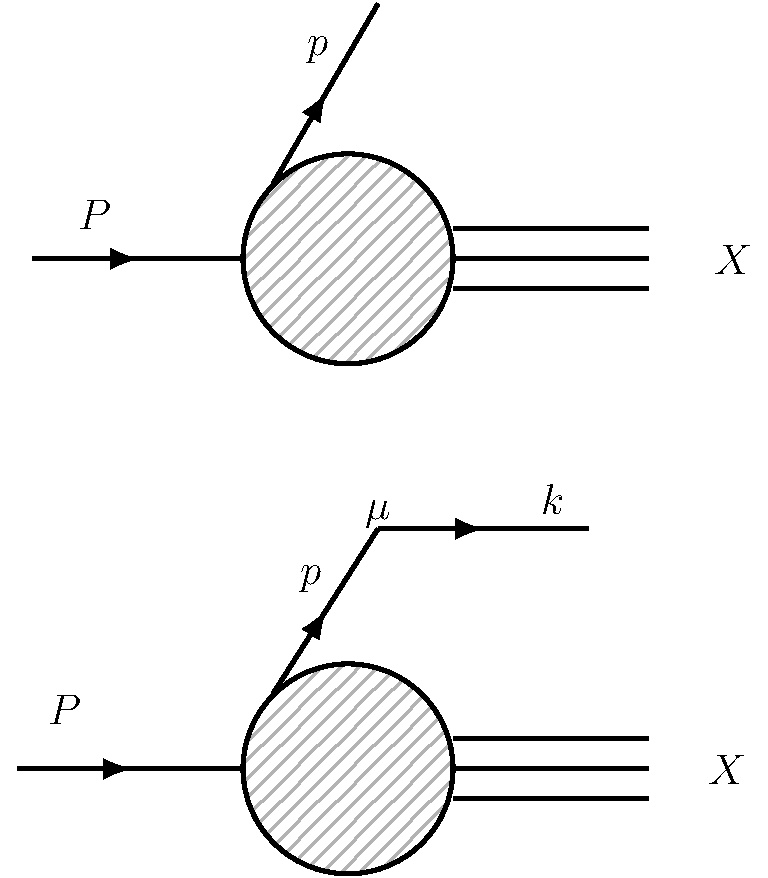
\includegraphics[scale=0.4]{Figures/HadronicTensor.pdf}
    \caption{Diagramatic construction of hadronic tensor}
    \label{fig:Hadronic tensor}
\end{figure}

To write down the hadronic tensor we integrate over the final states $X$ and $k$ and impose momentum conservation through a delta function. As usual, we use the exponential representation of the delta function, and the integral over $k$ will be made by using the on-shell condition, see \cref{eq:n-body phase space}
\begin{align}
    \int\frac{d^{3}k}{(2\pi)^{3}}\frac{1}{2k^{0}}=\int\frac{d^{4}k}{(2\pi)^{4}}2\pi\delta(k^{2}-m^{2})\theta(k^{0})\,,
\end{align}

Taking the quark to be massless, we find the hadronic tensor to take the form
\begin{align}
    W^{\mu\nu}&=4\pi^{3}\sum_{q}Q_{q}^{2}\sum_{X}\int\frac{d^{3}p_{X}}{(2\pi)^{3}2E_{X}}\int\frac{d^{3}k}{(2\pi)^{3}2k^{0}}\delta^{(4)}(P+q-k-p_{X})\nonumber
    \\
    &\hspace{0.8cm}\times\big(\gamma^{\mu}\slashed{k}\gamma^{\nu}\big)^{ji}\bra{P}\overline{\psi}_{j}(0)\ket{X}\bra{X}\psi_{i}(0)\ket{P}\nonumber
    \\
    &=4\pi^{3}\sum_{q}Q_{q}^{2}\sum_{X}\int\frac{d^{3}p_{X}}{(2\pi)^{3}2E_{X}}\int\frac{d^{4}k}{(2\pi)^{4}}2\pi\delta(k^{2})\theta(k^{0})\int\frac{d^{4}z}{(2\pi)^{4}}\,e^{iz\cdot(P-q-k-p_{X})}\nonumber
    \\
    &\hspace{0.8cm}\times\big(\gamma^{\mu}\slashed{k}\gamma^{\nu}\big)^{ji}\bra{P}\overline{\psi}_{j}(0)\ket{X}\bra{X}\psi_{i}(0)\ket{P}\nonumber
    \\
    &=\frac{1}{2}\sum_{q}Q_{q}^{2}\sum_{X}\int\frac{d^{3}p_{X}}{(2\pi)^{3}2E_{X}}\int d^{4}p\,\delta((p+q)^{2})\theta(p^{0}+q^{0})\nonumber
    \\
    &\hspace{0.8cm}\int\frac{d^{4}z}{(2\pi)^{4}}\,e^{iz\cdot(P-q-k-p_{X})}\big(\gamma^{\mu}(\slashed{p}+\slashed{q})\gamma^{\nu}\big)^{ji}\bra{P}\overline{\psi}_{j}(0)\ket{X}\bra{X}\psi_{i}(0)\ket{P}\,,
\end{align}
where we in the last step used that $k=p+q$, where $q$ is the photon momentum. By using the translation operator \cref{eq:translation operator} and the completeness relation \cref{eq:complete set of states}, we find
\begin{align}\label{eq:intermediate hadronic tensor}
    W^{\mu\nu}&=\frac{1}{2}\sum_{q}Q_{q}^{2}\int d^{4}p\,\delta((p+q)^{2})\theta(p^{0}+q^{0})\,\Phi_{ij}(p)\big(\gamma^{\mu}(\slashed{p}+\slashed{q})\gamma^{\nu}\big)^{ji}\nonumber
    \\
    &=\frac{1}{2}\sum_{q}Q_{q}^{2}\int d^{4}p\,\delta((p+q)^{2})\theta(p^{0}+q^{0})\,\text{tr}\Big(\Phi(p)\gamma^{\mu}(\slashed{p}+\slashed{q})\gamma^{\nu}\Big)\,,
\end{align}
where the quark correlator in momentum space is defined as
\begin{align}\label{eq:quark correlator}
    \Phi_{ij}(p)=\int\frac{d^{4}z}{(2\pi)^{4}}\,e^{-ip\cdot z}\bra{P}\overline{\psi}_{j}(z)\psi_{i}(0)\ket{P}\,.
\end{align}

We want to simplify the hadronic tensor further, which is easiest by using light-cone coordinates, see \cref{sec:Appendix Light-cone coordinates}. We can then parametrize the proton, quark and photon momenta as in \cref{eq:light-cone parametrization} and \cref{eq:light-cone photon momenta}. With this parametrization, we can expand the delta function in \cref{eq:intermediate hadronic tensor} in the following way
\begin{align}
    \delta((p+q)^{2})&=\delta(p^{2}+2p\cdot q+q^{2})\nonumber
    \\
    &=\delta(2p^{+}q^{-}+2p^{-}q^{+}-2p_{\perp}\cdot q_{\perp}-Q^{2})\nonumber
    \\
    &\approx\delta(2p^{+}q^{-}-Q^{2})\nonumber
    \\
    &=\delta(2P\cdot q\,\xi-2P\cdot q\,x)\nonumber
    \\
    &=\frac{1}{2P\cdot q}\delta(\xi-x)\,,
\end{align}
where we in the first step used that the quarks are massless, and in the third line we used that $p_{\perp}\ll Q^{2}$. To rewrite the argument we also used the Bjorken variable $x=Q^{2}/2P\cdot q$. We observe that this delta function fixes the momentum fraction to be equal the Bjorken-$x$, just as in the parton model calculation.  

The second simplification we can make is to use the fact that in the infinite momentum frame, the incoming photon hits the quark head-on. Then the outgoing quark will move in the $k^{-}$ direction, giving
\begin{align}
    \slashed{k}&=\slashed{p}+\slashed{q}= \gamma^{+}q^{-}+\mathcal{O}\Big(\frac{1}{P^{+}}\Big)\,,
\end{align}
and with these simplifications the hadronic tensor takes the form
\begin{align}\label{eq:simplified hadronic tensor}
    W^{\mu\nu}&=\frac{1}{2}\sum_{q}Q_{q}^{2}\int d^{4}p\,\delta^{+}((p+q)^{2})\,\text{tr}\Big[\Phi(p)\gamma^{\mu}(\slashed{p}+\slashed{q})\gamma^{\nu}\Big]\nonumber
    \\
    &=\frac{1}{4}\sum_{q}Q_{q}^{2}\int dp^{+}dp^{-}d^{2}p_{\perp}\,\frac{1}{P\cdot q}\,\text{tr}\big[\Phi(p)\gamma^{\mu}\gamma^{+}q^{-}\gamma^{\nu}\big]\delta(\xi-x)\nonumber
    \\
    &=\frac{1}{4}\sum_{q}Q_{q}^{2}\int d\xi dp^{-}d^{2}p_{\perp}\,\frac{P^{+}q^{-}}{P\cdot q}\,\text{tr}\big[\Phi(p)\gamma^{\mu}\gamma^{+}\gamma^{\nu}\big]\delta(\xi-x)\nonumber
    \\
    &=\frac{1}{4}\sum_{q}Q_{q}^{2}\,\text{tr}\big[\Phi(x)\gamma^{\mu}\gamma^{+}\gamma^{\nu}\big]\,,
\end{align}
where we have defined the fourier transformed integrated quark correlator
\begin{align}\label{eq:integrated quark correlator}
    \Phi_{ij}(x)&=\int dp^{-}d^{2}p_{\perp} \Phi_{ij}(x,p^{-},p_{\perp})\nonumber
    \\
    &=\int\frac{dz^{-}}{2\pi}\,e^{-ixP^{+}z^{-}}\bra{P}\overline{\psi}_{j}(0^{+},z^{-},0_{\perp})\psi_{i}(0)\ket{P}\,.
\end{align}

To find the quark parton distribution we use the light-cone contraction $\gamma^{\mu}\gamma^{+}\gamma_{\mu}=-2\gamma^{+}$, such that the trace in \cref{eq:simplified hadronic tensor} can be written as
\begin{align}
    \text{tr}[\Phi(x)\gamma^{\mu}\gamma^{+}\gamma^{\nu}]&=g^{\mu\nu}\text{tr}[\Phi(x)\gamma^{\mu}\gamma^{+}\gamma_{\mu}]\nonumber
    \\
    &=-2g^{\mu\nu}\text{tr}[\Phi(x)\gamma^{+}]\,.
\end{align}
Further, we use that $g^{\mu\nu}=g_{\perp}^{\mu\nu}-\big(n_{+}^{\mu}n_{-}^{\nu}+n_{+}^{\nu}n_{-}^{\mu}\big)$, see \cref{eq:trasnversal tensor}, and insert it into \cref{eq:simplified hadronic tensor}. This will give the following expression for the hadronic tensor
\begin{align}
    W^{\mu\nu}=-\frac{1}{2}g_{\perp}^{\mu\nu}\sum_{q}Q_{q}^{2}\,\text{tr}[\Phi(x)\gamma^{+}]+\big(n_{+}^{\mu}n_{-}^{\nu}+n_{+}^{\nu}n_{-}^{\mu}\big)\sum_{q}Q_{q}^{2}\,\text{tr}[\Phi(x)\gamma^{+}]\,,
\end{align}
and if we compare this expression to \cref{eq:2ndparametrized hadronic tensor}, we find that we must have
\begin{align}
    F_{1}(x)=\frac{1}{2}\sum_{q}Q_{q}^{2}\,\text{tr}[\Phi(x)\gamma^{+}]\,.
\end{align}
However, we already know from \cref{eq:collinear factorization parton model F_1} that this structure function is given by
\begin{align}
    F_{1}(x)=\frac{1}{2}\sum_{q}Q_{q}^{2}f_{q}(x)\,,
\end{align}
from which it follows that the operator definition for the integrated quark PDF is given by
\begin{align}\label{eq:unpolarized quark PDF}
    f_{q/P}(x)=\int\frac{dz^{-}}{4\pi}\,e^{-ixP^{+}z^{-}}\bra{P}\overline{\psi}(0^{+},z^{-},0_{\perp})\gamma^{+}\psi(0)\ket{P}\,,
\end{align}
where the subscript $f_{i/P}$ is the common notation for integrated PDFs of a parton with flavour $i$ inside the proton. From now we will not make this statement as it is implicit in the notation. 

Having found an expression for the parton distribution function in terms of matrix elements, let us take a closer look at how we can make these gauge invariant and subsequently used as a motivation for deriving perturbative distributions.



%%%%%%%%%%%%%%%%%%%%%%%%%%%%%%%%%%%%%%%%%%%%%%%%%%%%%%%%%%%%%%
\subsection{Gauge Invariant Parton Distributions}
The quark correlator in \cref{eq:quark correlator} is not gauge invariant, which can be made clear if we look at the gauge transformation of the fields. In general, fermionic fields transform under local gauge transformations as
\begin{align}
    \psi'(x)&=e^{ig\alpha^{a}(x)t^{a}}\psi(x)
    \\
    \overline{\psi}'(x)&=\overline{\psi}(x)e^{-ig\alpha^{a}(x)t^{a}}\,,
\end{align}
and as a consequence the quark correlator in momentum space transform as
\begin{align}
    \Phi'(p)=\int\frac{d^{4}z}{(2\pi)^{4}}\,e^{-ip\cdot z}\bra{P}\overline{\psi}(z)e^{-i\alpha^{a}(z)t^{a}}e^{ig\alpha^{a}(0)t^{a}}\psi(0)\ket{P}\,,
\end{align}
where the fields are defined at different space-time points and the exponentials inside the matrix element do not cancel. 

A similar problem appeared when trying to define a directional derivative of the fermionic fields in \cref{sec:Wilson lines and Wilson loops}. We used a Wilson line to parallel transport the fields such that they could be subtracted in a meaningful way, giving rise to a directional covariant derivative that ensured gauge invariance. The same procedure does not apply here, but in \cref{sec:Wilson lines and Wilson loops} we had that the Wilson line transformed under gauge transformation as
\begin{align}\label{eq:Wilson line transformation in operator section}
    \mathcal{U'}[y,x]=e^{ig\alpha^{a}(y)t^{a}}\mathcal{U}[y,x])e^{-ig\alpha^{a}(x)t^{a}}\,,
\end{align}
which is exactly the transformation we need to cancel the exponentials. So, let us define the following Wilson line
\begin{align}
    \mathcal{U}[z,0]=\mathcal{P}\exp\Big(-ig\int_{0}^{z}dy^{\mu}A_{\mu}(y)\Big)\,,
\end{align}
where it is understood that $A_{\mu}=A_{\mu}^{a}t^{a}$. We can then use the transformation property of the Wilson line to write down the gauge invariant quark correlator as
\begin{align}
    \Phi(p)=\int\frac{d^{4}z}{(2\pi)^{4}}\,e^{-ip\cdot z}\bra{P}\overline{\psi}(z)\mathcal{U}[z,0]\psi(0)\ket{P}\,.
\end{align}

The integrated quark correlator in \cref{eq:integrated quark correlator} has fields that are fixed along the $z^{-}$ direction, which mean that the quark correlator takes the form
\begin{align}
    \Phi(x)&=\int\frac{dz^{-}}{2\pi}\,e^{-ixP^{+}z^{-}}\bra{P}\overline{\psi}(0^{+},z^{-},0_{\perp})\mathcal{U}[z^{-},0]\psi(0)\ket{P}\,,
    \\
    \mathcal{U}[z^{-},0]&=\mathcal{P}\exp\Big(-ig\int_{0}^{z^{-}}dy^{-}A^{+}(0^{+},y^{-},0_{\perp})\Big)\,,
\end{align}
and it follows that the gauge invariant formulation of the quark parton distribution is 
\begin{align}\label{eq:gauge invaiant unpolarized quark PDF}
    f_{q/P}(x)&=\int\frac{dz^{-}}{2\pi}\,e^{-ixP^{+}z^{-}}\bra{P}\overline{\psi}(0^{+},z^{-},0_{\perp})\gamma^{+}\mathcal{U}(z^{-}\,;0)\psi(0)\ket{P}\,.
\end{align}

We observe that if we choose the light-cone gauge, $A^{+}=0$, the Wilson line is $\mathcal{U}[z^{-},0]=1$. Hence, we reduce the parton distribution to the one defined in \cref{eq:unpolarized quark PDF}, and as long as one stays in light-cone gauge the Wilson line can be neglected. 

For a complete treatment we will also give the operator definition of the gluon distribution. The calculation is very similar to the one we made for the quark distribution, but this is a higher order effect through boson-gluon fusion via a quark, so we will not make the explicit derivation here. If one starts in the light-cone gauge the Wilson line can be ignored, and the integrated gluon PDF can be found to be \cite{Ji_2005,Dominguez_2011},
\begin{align}\label{eq:gauge dependent gluon PDF}
    f_{g/P}(x)=\int\frac{dz^{-}}{2\pi}x P^{+}e^{-ixP^{+}z^{-}}\bra{P}A_{i}^{a}(z^{-})A_{i}^{a}(0)\ket{P}\,,
\end{align}
where $i=-,1,2$ as we have set $A^{+}=0$. 

We know from \cref{sec:Wilson lines and Wilson loops} that the gauge fields transform under gauge transformation as
\begin{align}
    A_{\mu}^{a}t^{a}\rightarrow \frac{i}{g}e^{ig\alpha^{a}t^{a}}D_{\mu}e^{-ig\alpha^{a}t^{a}}\,,
\end{align}
meaning that in the current form the gluon distribution is not gauge invariant. Because of the derivative it would not help if we naively insert a Wilson line as we did for the quark distribution. Let us instead investigate the field strength tensor $F_{\mu\nu}$, with the transformation
\begin{align}
    F_{\mu\nu}\rightarrow e^{ig\alpha^{a}t^{a}}F_{\mu\nu}e^{-ig\alpha^{a}t^{a}}\,,
\end{align}
which we observe transform in a similar fashion as the Wilson line in \cref{eq:Wilson line transformation in operator section}. However, it is not valid to just replace the gauge fields with the field strength. We observe that if we did, and inserted the same Wilson line as for the quark distribution, it would still not be gauge invariant. This is not surprising as the quark fields are defined in the fundamental representation, and the gluon fields in the adjoint representation of $SU(3)$. Therefore, we need to use a Wilson line in the adjoint representation, which we define as
\begin{align}
    \mathcal{U}_{ab}^{A}[z,0]=\mathcal{P}\exp{-ig\int_{0}^{z}dy^{\mu}A_{\mu}^{c}(y)(t^{c})_{ab}}\,,
\end{align}
where $(t^{c})_{ab}=-if^{abc}$ are the generators in the adjoint representation. If we insert this Wilson line between two field strength tensors, we would have a gauge invariant operator. We can then use the field strength and relate it to the gauge fields in the following standard way
\begin{align}\label{eq:}
    F_{\mu\nu}^{a}&=\partial_{\mu}A_{\nu}^{a}-\partial_{\nu}A_{\mu}^{a}+gf^{abc}A_{\mu}^{b}A_{\nu}^{c}\,,
\end{align}
and use that $A^{+}=0$, which gives
\begin{align}
    F_{+i}^{a}&=\partial_{+}A_{i}^{a}\,.
\end{align}
Inserting for $A_{i}$ into \cref{eq:gauge dependent gluon PDF} and integrating by parts yields the gauge invariant gluon PDF
\begin{align}
    f_{g/P}(x)=\int\frac{dz^{-}}{2\pi}\frac{1}{x P^{+}}e^{-ixP^{+}z^{-}}\bra{P}F_{a}^{+i}(z^{-})\mathcal{U}_{ab}^{A}[z^{-},0]F_{b}^{+i}(0)\ket{P}\,,
\end{align}
where the factor of $xP^{+}$ is common for even spin particles, i.e for bosons. There are several additional subtleties when dealing with gluon PDFs that we have not covered, so for more details see \cite{Dominguez_2011}.

%%%%%%%%%%%%%%%%%%%%%%%%%%%%%%%%%%%%%%%%%%%%%%%%%%
\subsection{Parton-in-Parton Distributions}\label{sec:lightcone parton in parton distributions}
In this section we will define one last object that we will have use for in \cref{chap:Resummation in QCD}, namely \emph{parton-in-parton} distributions. As we shall see, these will be useful when we want to renormalize our hadron--hadron cross-section and when we want to refactorize the cross-section in the so-called \emph{threshold region}, making it eligible for resummation. 


To define the parton-in-parton distribution we start from the quark PDF \cref{eq:unpolarized quark PDF} and insert a complete set of final states in the following way
\begin{align}
    f_{q/P}(x)&=\int\frac{dz^{-}}{4\pi}\,e^{-ixP^{+}z^{-}}\bra{P}\overline{\psi}(0^{+},z^{-},0_{\perp})\gamma^{+}\psi(0)\ket{P}\nonumber
    \\
    &=\int\frac{dz^{-}}{4\pi}\,e^{-iz^{-}(P_{n}^{+}-P^{+}+xP^{+})}\sum_{n}\bra{P}\overline{\psi}(0)\ket{n}\gamma^{+}\bra{n}\psi(0)\ket{P}\nonumber
    \\
    &=\frac{1}{2}\sum_{n}\bra{P}\overline{\psi}(0)\ket{n}\gamma^{+}\bra{n}\psi(0)\ket{P}\,\delta(P_{n}^{+}-(1-x)P^{+})\,,
\end{align}
where we used the translation operator to pick out the momentum $P_{n}^{+}-P^{+}$ in the exponential, see \cref{eq:translation operator}. It is understood that the matrix element is an average and sum over spin, as $f_{q/P}$ is by construction unpolarized. Let us then consider the case where $P=q$, i.e. a quark. In that case we must also include an average and sum over colour. Then we can naively write down the quark-in-quark distribution as
\begin{align}\label{eq:expanded matrix element quark-in-quark}
    f_{q/q}(x)&=\frac{1}{4N_c}\sum_{colour}\sum_{spin}\sum_{n}\bra{q}\overline{\psi}(0)\ket{n}\gamma^{+}\bra{n}\psi(0)\ket{q}\,\delta(p_{n}^{+}-(1-x)p^{+})\,,
\end{align}
where we have explicitly written out the average and sum over colour and spin. To evaluate the matrix elements we use that if a quark operator $\psi$ act on a quark state $\ket{q}$, we get
\begin{align}\label{eq:quark operator on quark state}
    \psi(z)\ket{q}=e^{-ip\cdot z}u(p)\ket{0}\,,
\end{align}
which mean that the matrix elements in \cref{eq:expanded matrix element quark-in-quark} only have a contribution if $n=0$. This scenario corresponds to a quark that just \textquote{travels} along without changing. Thus, we conclude that the expression we have written down is the leading order expansion of $f_{q/q}$, where there is no gluon radiation from the quark line. It is therefore important to point out that the only way a quark can \textquote{change} is by radiating a gluon, and in this scenario there is no gluon to make that change. Hence, by using \cref{eq:quark operator on quark state}, we find the leading order result for the quark-in-quark distribution,
\begin{align}
    f_{q/q}^{(0)}(x)&=\frac{1}{4p^{+}}\sum_{s}u_{i}^{s}(p)\bar{u}_{j}^{s}(p)\gamma_{ji}^{+}\,\delta(1-x)\nonumber
    \\
    &=\frac{1}{4p^{+}}\text{tr}[\slashed{p}\gamma^{+}]\delta(1-x)\nonumber
    \\
    &=\delta(1-x)\,,
\end{align}
which states that in the absence of interaction the quark remains itself. For general partons, we can therefore write 
\begin{align}
    f_{i/j}^{(0)}(x)=\delta_{ij}\delta(1-x)\,,
\end{align}
where $\delta_{ij}$ is inserted to make sure that the parton does not change without a gauge interaction. If we assume that $f_{i/j}$ can be calculated in perturbation theory, the expansion take the form
\begin{align}
    f_{i/j}(x,\mu^{2})=\delta_{ij}\delta(1-x)+\sum_{n=1}^{\infty}\Big(\frac{\alpha_s}{2\pi}\Big)^{n}f_{i/j}^{(n)}(x,\mu^{2})\,.
\end{align}

Before we proceed to the general treatment of radiation from quark lines, we can actually \textquote{guess} the first order correction. In \cref{sec:QCD and Collinear factorization} we calculated a diagram where a gluon was emitted from an incoming quark line, see \cref{fig:DISgluonemission}. The divergent part of the diagram was found to be  
\begin{align}
    \hat{F}_{2}\big|_{\text{div}}=Q_{q}^{2}\,\frac{\alpha_s}{2\pi}x\,P_{q/q}^{(0)}(x)\ln{\frac{Q^{2}}{Q_{0}^{2}}}\,,
\end{align}
where the quark--quark splitting function naturally appeared as the process involved a quark emitting a gluon and continued on as another quark. Thus, if $f_{q/q}^{(1)}$ describes a quark emitting a gluon and continuing on as another quark, the natural guess would be
\begin{align}\label{eq:momentum cut-off quark-in-quark}
    f_{q/q}^{(1)}(x)\propto P_{q/q}^{(0)}(x)\,,
\end{align}
i.e. it has to be proportional to the splitting functions as it describes exactly what the splitting function describes.

For the general treatment, we need to implement gauge interactions systematically. But we already know from \cref{sec:Wilson lines and Wilson loops} that this can be done by dressing the quark line with a Wilson line. Therefore, we can use our expression for the gauge invariant parton distributions, see \cref{eq:gauge invaiant unpolarized quark PDF}, and expand the Wilson line. To do this, we can first use the Wilson line relation
\begin{align}
    \mathcal{U}[z,0]=\mathcal{U}^{\dagger}[+\infty,z]\mathcal{U}[+\infty,0]\,,
\end{align}
and use \cref{eq:eq:wilso dress fermion} to write
\begin{align}
    \Psi(z)=\mathcal{U}[\infty,0]\psi(z)\,,
    \\
    \overline{\Psi}(z)=\bar{\psi}(z)\mathcal{U}^{\dagger}[\infty,z]\,.
\end{align}

With these definitions the quark-in-quark distribution can be defined as 
\begin{align}
    f_{q/q}(x)=\int\frac{dz^{-}}{4\pi}e^{-ixp^{+}z^{-}}\bra{q}\overline{\Psi}(z^{-})\gamma^{+}\Psi(0)\ket{q}\,,
\end{align}
also commonly rewritten by inserting a complete set of states, giving
\begin{align}\label{eq:Collins definition of parton-in-parton}
    f_{q/q}(x)=\int\frac{dz^{-}}{4\pi}e^{-ixp^{+}z^{-}}\sum_{n}\bra{q}\overline{\Psi}(z^{-})\ket{n}\gamma^{+}\bra{n}\Psi(0)\ket{q}\,.
\end{align}

The expansion of a semi-infinite Wilson line is given in \cref{eq:path bounded from above} and \cref{eq:path bounded from below}, from which \cref{eq:Collins definition of parton-in-parton} can be calculated in perturbation theory. We will not perform this calculation explicitly, but we can find its pole structure by comparing with the amplitude in \cref{eq:Dressed fermion amplitude}. When squaring this amplitude, one finds that the $\mathcal{O}(g
^{2})$ term describes a scaleless integral. Scaleless integrals has the pole structure given in \cref{eq:scaleless integral}. The UV-divergence can be removed by counterterms, leaving the IR-divergence in $1/\epsilon$. An explicit calculation to $\mathcal{O}(\alpha_s)$ in dimensional regularization gives \cite{Collins:1989gx},
\begin{align}\label{eq:quark in quark PDF to one-loop}
    f_{q/q}(x)=\delta(1-x)-\frac{\alpha_s}{2\pi}\Big(\frac{4\pi\mu^{2}}{\mu_{F}^{2}}\Big)^{\epsilon}\frac{\Gamma(1-\epsilon)}{\Gamma(1-2\epsilon)}\frac{1}{\epsilon}P_{q/q}^{(0)}(x)+\mathcal{O}(\alpha_{s}^{2})\,,
\end{align}
where the $1/\epsilon$ factor appear as a consequence of a collinear singularity. From these considerations it follows that the first order correction $f_{q/q}^{(1)}$ has the structure given in \cref{eq:momentum cut-off quark-in-quark}. We could also have gluons or quarks radiating from a gluon in the initial state, and the same arguments would apply with the difference in which splitting function that would appear in the expression. We should emphasize that there are several ways of defining these parton-in-parton distributions. The choice made in \cref{eq:Collins definition of parton-in-parton} are lightcone distributions with a fixed momentum fraction. In \cref{sec:Resummation Drell-yan} we will define distributions at fixed energy instead, which make them more suitable for resummation. The most important point here is that one can use these parton-in-parton distributions to absorb collinear singularities that appear when gluons radiate from quark lines in scattering processes. This is a very important feature when doing resummation that will be used on several occasions. 

   






 


% \section{Drell-Yan Cross Section in QCD}\label{sec:Drell-Yan Hadronic Cross Section}
In this section we will make another calculation that historically has been important in the study of QCD, namely the Drell-Yan process.  

In 1970, the first observation of a $\mu^{+}\mu^{-}$ in hadron-hadron collision was observed \cite{Christenson:1970um}. By applying the parton model Drell and Yan were the first to give a theoretical prediction of this process \cite{Drell:1970wh}. In the modern framework of QCD, the impulse approximation of the parton model is as in DIS replaced by the more precise concept of factorization. Then it can be proven that the hadronic Drell-Yan cross section can be written as a convolution of a perturbative calculable partonic cross section and universal process independent parton distribution functions \cite{Collins:1989gx}. Without specifying the kinematics, the hadronic cross section can be written as
\begin{align}
  \sigma_{h_1\,h_2}(P_1,P_2)=\sum_{i,j}\int dx_1\,dx_2\,f_{i/h_1}(x_1,\mu_{F})f_{j/h_1}(x_1,\mu_{F})\,\hat{\sigma}_{ij}(x_1P_1,x_2P_2,\mu_{F})\,,
\end{align}
which is the form we expected from the parton model, and as in DIS, the parton distribution functions and the partonic cross section has acquired an dependancy on the factorization scale. 

In the simplest case, a Drell-Yan process is the annihilation of a quark-antiquark pair into a virtual photon, which subsequently produces a pair of leptons with invariant mass $Q^{2}$. As leptons are blind to the strong interaction, there will not be any final state gluon radiation. The consequence is that all radiation comes from the initial state quark-antiquark pair, and therefore we have a clear probe of the behaviour of coloured particles. Consequently, the Drell-Yan process is an effective way of studying the internal structure of hadrons.

The main objective of this section is to investigate the divergences appearing in higher-order calculations, and how to deal with them using renormalization techniques. The calculation will proceed through the use of dimensional regularization, where the poles will manifest themselves in $1/\epsilon$. Further, close to the threshold, the finite result has contributions that become large, and these must eventually be handled using resummation techniques. To this end, we will focus on the next-to-leading order (NLO) calculation, where the initial state quarks emit a gluon.

\subsection{LO Drell-Yan Cross Section}
For the sake of completeness we will first sketch the leading order result. At this order we write the partonic process as $q(p)+\bar{q}(p')\rightarrow l^{-}(k)+l^{+}(k')$, where the corresponding Feynman diagram is given in \cref{fig:Drell-Yan LO}.
\begin{figure}
  \centering
  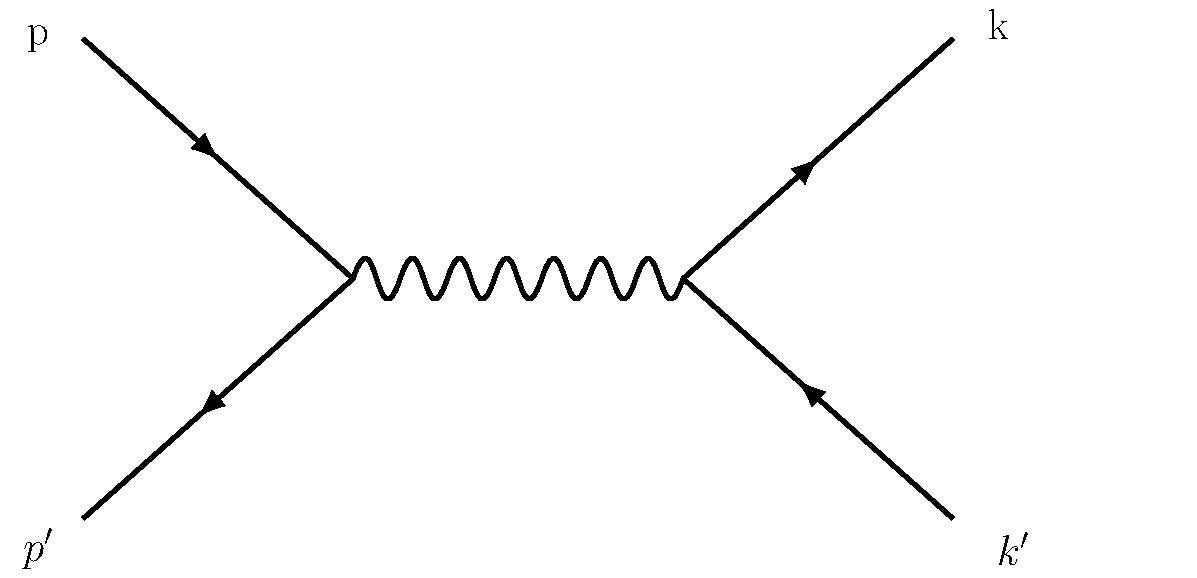
\includegraphics[scale=0.4]{Figures/DrellYanLO}
  \caption{Drell-Yan process at leading order.}
  \label{fig:Drell-Yan LO}
\end{figure}\noindent
Here $p$ and $p'$ denote the momenta of the incoming quark and antiquark, and likewise $k$ and $k'$ denote the momentum of the outgoing leptons. We can directly write down the amplitude from the basic Feynman rules\footnote{To see where all these term comes from, see \cref{eq:QED feynman rule} for the quark-photon vertex, \cref{eq:photon propagator without gauge choice} for the photon propagator and \cref{sec:canonical quantization free theories} for the appearance of spinors.}
\begin{align}
    i\mathcal{M}=i\delta_{ij}\frac{Q_{q}e^{2}}{q^{2}}\big[\bar{v}(p')\gamma^{\mu}u(p)\big]\big[\bar{u}(k)\gamma_{\mu}v(k')\big]\,,
\end{align}
where $\delta_{ij}$ is a colour conserving factor for the quark vertex, and $Q_{q}$ is the fractional charge of the quarks. As usual we are only interested in the spin and colour averaged amplitude,
\begin{align}
    \langle\,|\mathcal{M}|^{2}\rangle=\frac{1}{N_{c}N_{s}^{2}}\frac{Q_{q}^{2}e^{4}}{\hat{s}^{2}}H^{\mu\nu}L_{\mu\nu}\,,
\end{align}
where $N_c$ and $N_s$ denote the number of colours and spin, and we  have defined hadronic and leptonic tensors
\begin{align}
    H^{\mu\nu}&=\text{Tr}\big[\slashed{p'}\gamma^{\mu}\slashed{p}\gamma^{\nu}\big]\,,
    \\
    L_{\mu\nu}&=\text{Tr}\big[\slashed{k}\gamma_{\mu}\slashed{k'}\gamma_{\nu}\big]\,,
\end{align}
and the contraction yields
\begin{align}
    H^{\mu\nu}L_{\mu\nu}=\hat{s}^{2}(1+\cos\theta^{2})\,,
\end{align}
where $\theta$ is the centre of mass scattering angle, and $\hat{s}$ is the partonic centre of mass energy, $\hat{s}=(p+p')^{2}$. The differential cross section is given by
\begin{align}
    d\hat{\sigma}_{q\bar{q}}^{(0)}=\frac{1}{2\hat{s}}\langle\,|\mathcal{M}|^{2}\rangle d\mathcal{P}^{(2)}\,,
\end{align}
where $d\mathcal{P}^{(2)}$ is the two-body phase space of the final state leptons, see \cref{eq:n-body phase space}. The integrated cross section is given by
\begin{align}
    \hat{\sigma}^{(0)}=\frac{4\pi Q_{q}^{2}\alpha^{2}}{3N_{c}\hat{s}}\,.
\end{align}
We can write this as a differential cross section by using that
\begin{align}
    1=\int dQ^{2}\delta(\hat{s}-Q^{2})\,,
\end{align}
which is merely a statement that the invariant mass of the $q\bar{q}$ pair that annihilates into the photon, matches the invariant mass of the photon. This identity can also be written on the form
\begin{align}
    1=\frac{1}{\hat{s}}\int dQ^{2}\delta(1-\frac{Q^{2}}{\hat{s}})\,,
\end{align}
giving the differential cross section in $Q^{2}$
\begin{align}
    \frac{d\hat{\sigma}_{q\bar{q}}^{(0)}}{dQ^{2}}=\frac{4\pi Q_{q}^{2}\alpha^{2}}{3N_{c}\hat{s}\,Q^{2}}\delta(1-z)=\hat{\sigma}_{0}\,\delta(1-z)\,,
\end{align}
where we defined the partonic Born cross-section $\hat{\sigma}_0=(4\pi Q_{q}^{2}\alpha^{2})/(3N_{c}\hat{s}Q^{2})$, and the partonic threshold variable $z=Q^{2}/\hat{s}$. For later purposes, we want to make some remarks about the structure of the leading order diagram. The photon and leptons do not feel the strong interaction, which means that even at higher orders, the final state part of the amplitude decouples from the initial part. Further, the electromagnetic corrections are negligible compared to the strong corrections so any photon radiation is neglected. To find the higher-order corrections, we only have to consider the corrections for the production of a virtual photon. The leptonic part of the hard process contributes with a factor $\alpha/3Q
^{2}$, where $Q^{2}$ is the invariant mass of the final state leptons.

\begin{figure}
    \centering
    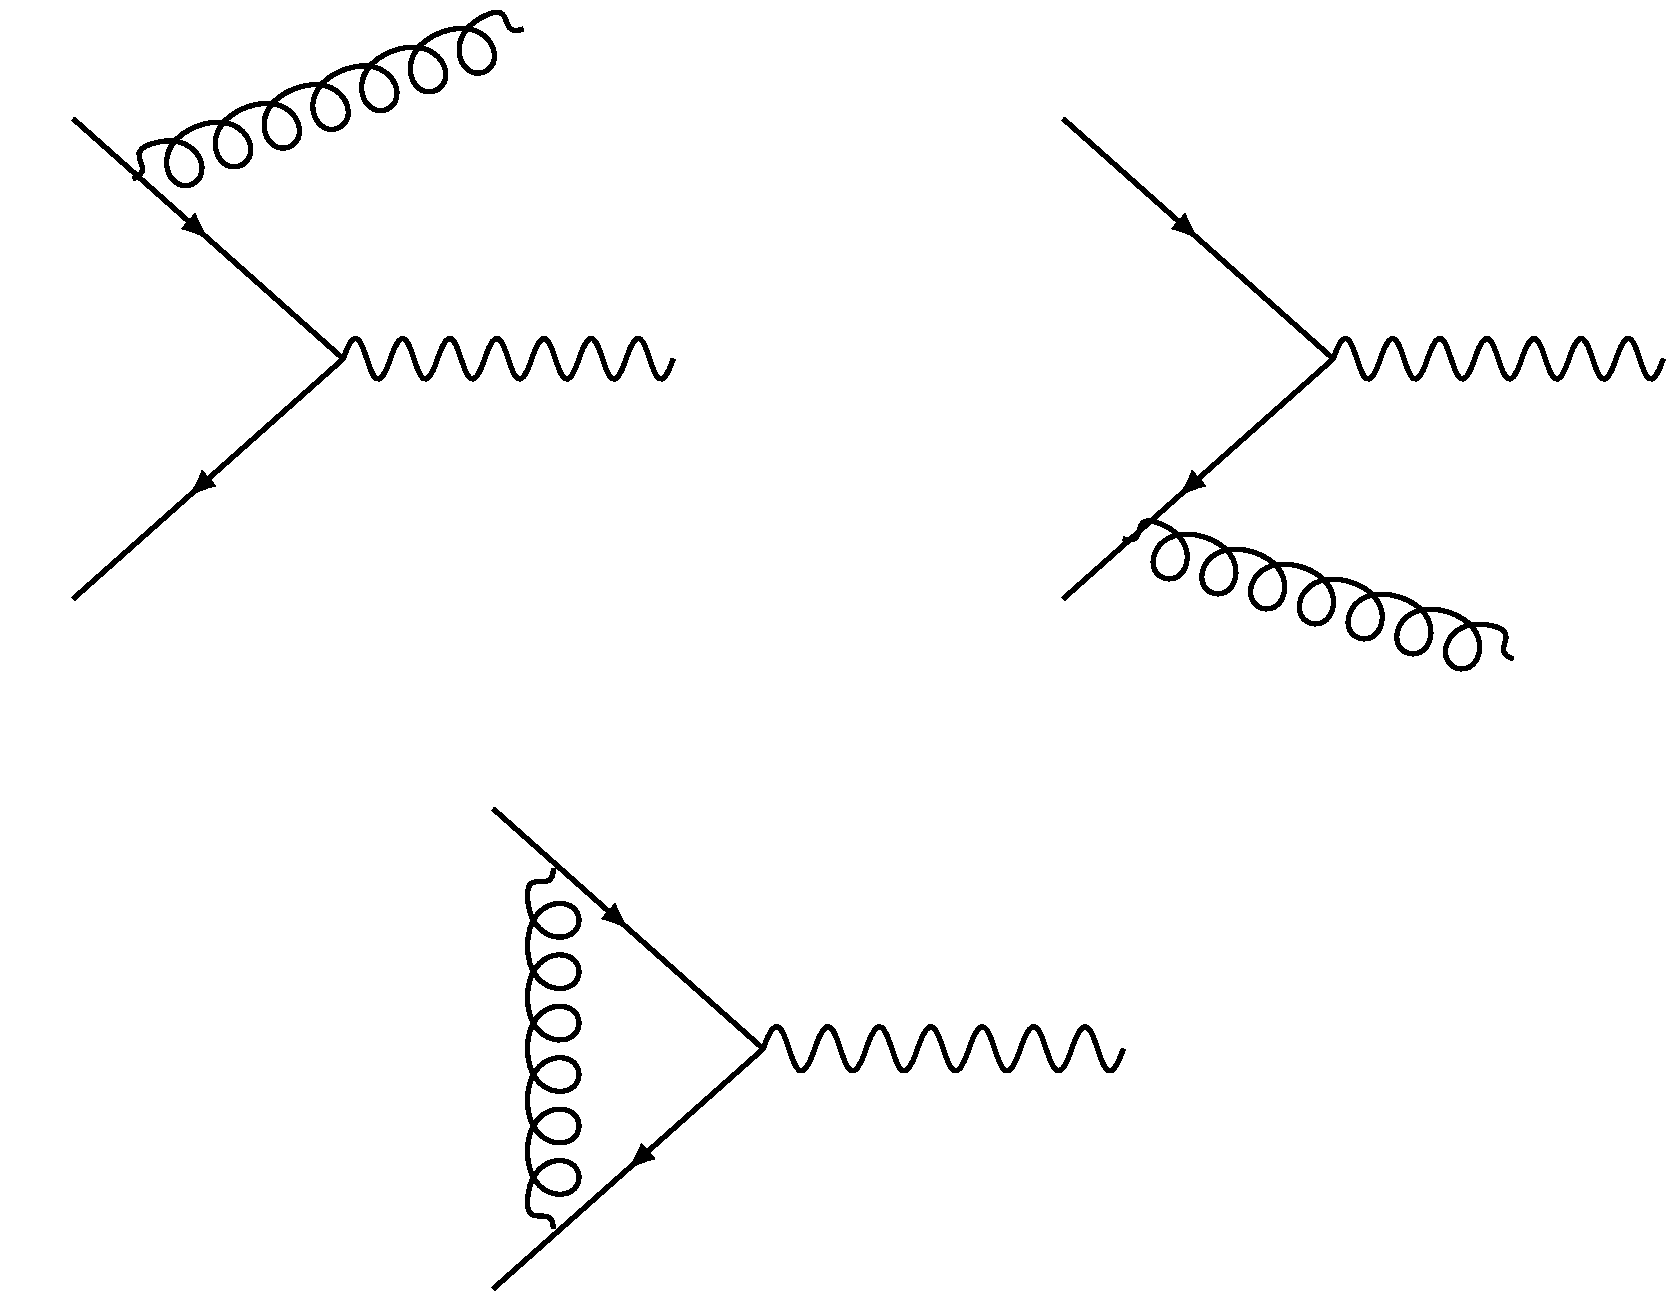
\includegraphics[scale=0.3]{Figures/radiativecorrDY.pdf}
    \caption{NLO diagrams contributing to the Drell-Yan process. Top: Real gluon emission. Bottom: Virtual correction.}
    \label{fig:NLO drell-yan}
\end{figure}
%%%%%%%%%%%%%%%%%%%%%%%%%%%%%%%%%%%%%%%%%%%%%%%%%%%%%%%%%%%%%%%%%%
\subsection{NLO Drell-Yan Cross Section}\label{sec:NLO drell yan calculation}
Let us now go beyond the leading order approximation and calculate the $\mathcal{O}(\alpha_s)$ correction to the Drell-Yan process. The contributing diagrams is illustrated in \cref{fig:NLO drell-yan}, where the upper diagrams corresponds to real gluon emission, and the lower diagram is the virtual correction. As we will see, the difficulty due to divergences in the integral is substantial. To treat these divergences we will use dimensional regularization, see \cref{sec:dimensional regularization} for more detail. One important feature to keep in mind is that the UV-divergences is treated by evaluating $\epsilon>0$ and the IR-divergences for $\epsilon<0$. 

Now, by counting order in $g_s$ in \cref{fig:NLO drell-yan}, we see that the virtual correction has one order higher than the real emission and can not be squared in order to contribute to NLO. Therefore, one must multiply the virtual correction amplitude with the leading order amplitude found from \cref{fig:Drell-Yan LO}, which contributes to wanted order in $\alpha_s$.
The real contribution corresponds to the emission of gluons that are on mass-shell, i.e. there are no undetermined loop momenta that has to be integrated over. However, the phase space integration contains two kinds of singularities. The first is when the gluon is emitted collinearly to the emitting quark. The second singularity appears if the gluon momentum is soft, $k\rightarrow 0$. Both of these divergences are what is called infrared-singularities. Virtual corrections emerge when the initial quarks exchange a gluon. This gluon is virtual, and the integral is over undetermined loop momenta, leading to ultraviolet-divergences. To handle these divergences, we will use dimensional regularization, and work in $d=4-2\epsilon$ dimensions.

\subsection*{Differential cross section}
By applying the QCD Feynman rules, the amplitude for real gluon emission can be written as
\begin{align}
    i\mathcal{M}=&Q_{q}\,e\,g_{s}\,\mu^{(4-d)/2}\,(t^{a}_{ij})\varepsilon_{\alpha}^{*}(k)\varepsilon_{\mu}^{*}(q)\big[\bar{v}(p')A^{\mu\alpha}u(p)\big]\,,
\end{align}
where we have made the usual substitution $g_{s}\rightarrow \mu^{\epsilon}g_s$. We have also used the abbreviation
\begin{align}
    A^{\mu\alpha}=\gamma^{\mu}\frac{i(\slashed{p}-\slashed{k})}{(p-k)^{2}}\gamma^{\alpha}+\gamma^{\alpha}\frac{i(\slashed{p}-\slashed{q})}{(p-q)^{2}}\gamma^{\mu}\,,
\end{align}
where $k$ is the gluon momenta and $q$ is the massive photon momenta. The spin and colour averaged amplitude is given by
\begin{align}\label{eq:ugly NLO averaged amplitude DY}
    \langle\,|\mathcal{M}|^{2}\rangle&=\mathcal{C}\frac{Q_{q}^{2}e^{2}g_{s}^{2}\mu^{(4-d)}}{N_{s}^{2}}\text{Tr}[\slashed{p'}A^{\mu\alpha}\slashed{p}A_{\alpha\mu}]\nonumber
    \\
    &=C_{F}\frac{Q_{q}^{2}e^{2}g_{s}^{2}\mu^{(4-d)}}{N_{c}\,N_{s}^{2}}\,2(d-2)\Big(2\hat{s}\frac{Q^{2}}{\hat{t}\hat{u}}+2(d-4)+(d-2)\Big[\frac{\hat{t}}{\hat{u}}+\frac{\hat{u}}{\hat{t}}\Big]\Big)\nonumber
    \\
    &=C_{F}\frac{Q_{q}^{2}e^{2}g_{s}^{2}\mu^{2\epsilon}}{N_{c}\,N_{s}^{2}}\,8(1-\epsilon)\Big(2\hat{s}\frac{Q^{2}}{\hat{t}\hat{u}}-2\epsilon+(1-\epsilon)\Big[\frac{\hat{t}}{\hat{u}}+\frac{\hat{u}}{\hat{t}}\Big]\Big)\,,
\end{align}
where the terms with $d=4-2\epsilon$ appears because of the modified Dirac algebra in $d$-dimensions \cref{sec:Appendix Dirac gamma matrices}. The color factor for this process follows from the QCD group structure\footnote{See \cite{Peskin:257493} for a more elaborate treatment of the colour sums.} 
\begin{align}
    \mathcal{C}=\frac{1}{N_{c}}\text{Tr}[t^{a}t^{a}]=\frac{C_{F}}{N_C}\,,
\end{align}
and the partonic Mandelstam variables is defined as
\begin{align}\label{eq:partonic Mandelstam}
    \hat{s}&=(p+p')^{2}=(q+k)^{2}\,,
    \\
    \hat{t}&=(p-q){2}=(p'-k)^{2}\,,
    \\
    \hat{u}&=(p-k)^{2}=(p'-q)^{2}\,.
\end{align}
The partonic differential cross section is then given by
\begin{align}
    \frac{d\hat{\sigma}_{q\bar{q}}^{r}}{dQ^{2}}=\frac{1}{2}\Big(\frac{\alpha}{3Q^{2}}\Big)\int\,d\mathcal{P}^{(2)}\,\langle\,|\mathcal{M}|^{2}\rangle\,,
\end{align}
where the bracket represents lepton part appearing at all order. The differential phase space is over the massless gluon momenta $k$ and the virtual photon momenta $q$. In $d$-dimensions, the differential phase space can be written as
\begin{align}
    d\mathcal{P}=\frac{1}{8\pi}\Big(\frac{4\pi}{Q^{2}}\Big)^{\epsilon}\frac{(1-z)^{1-2\epsilon}\,z^{\epsilon}}{\Gamma(1-\epsilon)}\big(y(1-y))\big)^{-\epsilon}\,dy\,,
\end{align}
where $y=\frac{1}{2}(1+\cos\theta)$, $\Gamma$ is the Euler-Gamma function and z is the threshold variable $z=Q^{2}/\hat{s}$. Notice that the integral is to be taken over the dimensionless quantity $y$, so we should find a way of rewriting the averaged amplitude in terms $y$ as well. We already have the partonic centre of mass-energy, $\hat{s}$ in terms of $z$, so by writing out $\hat{t}$ and $\hat{u}$ we find
\begin{align}
    \hat{t}&=-\frac{Q^{2}}{z}(1-z)(1-y)\,,
    \\
    \hat{u}&=-\frac{Q^{2}}{z}(1-z)y\,.
\end{align}
With these definitions, the averaged amplitude in \cref{eq:ugly NLO averaged amplitude DY} takes the form
\begin{align}
     \langle\,|\mathcal{M}|^{2}\rangle&=C_{F}\frac{Q_{q}^{2}e^{2}g_{s}^{2}\mu^{2\epsilon}}{N_{c}\,N_{s}^{2}}\,8(1-\epsilon)\Big(\frac{2z}{(1-z)^{2}(1-y)y}\nonumber
     \\
     &\hspace{0.2cm}+(1-\epsilon)\Big[\frac{1-y}{y}+\frac{y}{1-y}\Big]-2\epsilon\Big)\,.
\end{align}
At this point it is worth commenting the different terms in this expression: we have that $(1-z)$ is the momentum fraction of the emitted gluon, and if the gluon is soft, $z=1$, we have a singularity. Further, if the gluon is emitted collinearly to the emitting quarks, we have that $y=1$, resulting in another singularity. Hence, we have both a collinear and soft divergence.

However, if we keep $\epsilon$ finite, the singularities can be extracted by using the Euler-Beta integral. The singularities will then manifest themselves in $\epsilon$ singularities. Writing out all terms, the differential cross-section for real emission takes the form
\begin{align}
    \frac{d\hat{\sigma}_{q\bar{q}}^{r}}{dQ^{2}}&=\frac{1}{2\hat{s}}\Big(\frac{\alpha}{3\pi Q^{2}}\Big)\Big[C_{F}\frac{Q_{q}^{2}e^{2}g_{s}^{2}\mu^{2\epsilon}}{N_{c}\,N_{s}^{2}}\Big]\frac{1}{8\pi}\Big(\frac{4\pi}{Q^{2}}\Big)^{\epsilon}\frac{(1-z)^{1-2\epsilon}\,z^{\epsilon}}{\Gamma(1-\epsilon)}8(1-\epsilon)\nonumber
    \\
    &\hspace{0.3cm}\times\int_{0}^{1}dy\,\big(y(1-y)\big)^{-\epsilon}\Big(\frac{2z}{(1-z)^{2}(1-y)y}+(1-\epsilon)\Big[\frac{1-y}{y}+\frac{y}{1-y}\Big]-2\epsilon\Big)\nonumber
    \\
    &=C_{F}\hat{\sigma}_{0}\frac{\alpha_s}{2\pi}\Big(\frac{4\pi\mu^{2}}{Q^{2}}\Big)^{\epsilon}\frac{(1-\epsilon)}{\Gamma(1-\epsilon)}(1-z)^{1-2\epsilon}z^{\epsilon}\nonumber
    \\
    &\hspace{0.3cm}\times\Big[\frac{2z}{(1-z)^{2}}B(-\epsilon,-\epsilon)+2(1-\epsilon)B(-\epsilon,2-\epsilon)-2\epsilon B(1-\epsilon,1-\epsilon)\Big]\nonumber
    \\
    &=C_{F}\hat{\sigma}_{0}\frac{\alpha_s}{\pi}A(\epsilon)\frac{z^{\epsilon}}{\epsilon}\Big(-2z(1-z)^{-1-2\epsilon}-(1-z)^{1-2\epsilon}\Big)\,,
\end{align}
where we for notational simplicity have neglected several factors that are finite for $\epsilon\rightarrow 0$. The integral over $y$ was performed by the Euler-Beta integral
\begin{align}
    B(a,b)=\int_{0}^{1}dt\,t^{a-1}(1-t)^{b-1}=\frac{\Gamma(a)\Gamma(b)}{\Gamma(a+b)}\,,
\end{align}
and we defined the prefactor $A(\epsilon)$ as
\begin{align}
    A(\epsilon)=\Big(\frac{4\pi\mu^{2}}{Q^{2}}\Big)^{\epsilon}\frac{\Gamma(1-\epsilon)}{\Gamma(1-2\epsilon)}\,.
\end{align}

We still have a singularity as $z\rightarrow 1$. To make all singularities manifest in $\epsilon$, we can expand the terms inside the bracket by the use of plus distributions, see \cref{sec:Appendix Plus Distributions}. We write this as
\begin{align}\label{eq:DRell Yan plus distribution example}
    (1-z)^{-1-2\epsilon}&=-\frac{1}{2\epsilon}\delta(1-z)+\Big[\frac{1}{1-z}\Big]_{+}-2\epsilon\Big[\frac{\ln(1-z)}{1-z}\Big]_{+}+\mathcal{O}(\epsilon^{2})\,,
    \\
    z^{\epsilon}&=1+\epsilon \ln z+\mathcal{O}(\epsilon^{2})\,.
\end{align}
With these considerations, the final result for real gluon emission takes the form
\begin{align}
    \frac{d\hat{\sigma}_{q\bar{q}}^{r}}{dQ^{2}}=C_{F}&\hat{\sigma}_{0}\frac{\alpha_s}{\pi}A(\epsilon)\Big(\frac{1}{\epsilon^{2}}\delta(1-z)-\frac{1}{\epsilon}\Big[\frac{1+z^{2}}{1-z}\Big]_{+}\,,\nonumber
    \\
    &+2(1+z^{2})\Big[\frac{\ln(1-z)}{(1-z)}\Big]_{+}-\frac{1+z^{2}}{1-z}\ln z\Big)\,.
\end{align}

We have now managed to bring all singularities on $\epsilon$ form. The term $1/\epsilon^{2}$ is an infrared singularity due to simultaneously soft and collinear emission, and the term $1/\epsilon$ is due to collinear emission. 

To any given order in perturbation theory, we must consider all possible diagrams at that specific order and add them at the end. Therefore, we must find the virtual contribution and see if some of the singular terms cancel. The only virtual contribution comes from the lower diagram in \cref{fig:NLO drell-yan}. There are two additional diagrams at this order that could contribute, the quark self-energy diagrams, but it can be shown that these exactly cancel each other. The virtual contribution contains both infrared and ultraviolet-singularities. To separate these singularities, we do as in \cref{eq:scaleless integral} and name them $\epsilon_{UV}$ and $\epsilon_{IR}$. 

The amplitude for the virtual correction is given by
\begin{align}\label{eq:DY virtual amplitude}
    \mathcal{M}^{\mu}=&t_{ik}^{a}t_{kj}^{a}\mu^{(4-d)}\int\frac{d^{d}k}{(2\pi)^{2}}\bar{v}(p')(ig_s\gamma^{\alpha})\frac{i(\slashed{p'}+\slashed{k})(ie\gamma^{\mu})i(\slashed{k}-\slashed{p}))}{(p'+k)^{2}(p-k)^{2}}(ig_s\gamma^{\beta})u(p)\,D_{\alpha\beta}(k)\nonumber
    \\
    &=eg_s^{2}C_{F}\mu^{(d-4)}\int\frac{d^{d}k}{(2\pi)^{2}}\bar{v}(p')\gamma^{\alpha}\frac{(\slashed{p'}+\slashed{k})\gamma^{\mu}(\slashed{k}-\slashed{p})}{k^{2}(p'+k)^{2}(p-k)^{2}}\gamma^{\beta}u(p)\nonumber
    \\
    &=\bar{v}(p')(\Gamma^{\mu})u(p)\,,
\end{align}
where we have defined the vertex correction $\Gamma^{\mu}$. The integrand can be simplified by the Dirac algebra in $d$-dimensions and the massless Dirac equation. Further, by applying the Feynman parameter method introduced in \cref{sec:dimensional regularization}, the integral can be turned into a Euler-Beta integral. 

The propagator factors in \cref{eq:DY virtual amplitude}, are the same as the ones we derived in \cref{eq:virtual gluon feynman parametrization}. The numerator is straightforward to manipulate, but tedious. The resulting vertex correction is given by
\begin{align}
    \Gamma^{\mu}=\gamma^{\mu}&C_{F}\frac{\alpha_s}{4\pi}\Big(\frac{4\pi\mu^{2}}{Q^{2}}\Big)^{\epsilon}(-1)^{\epsilon}\Gamma(1+\epsilon)\Gamma(1-\epsilon)\frac{\Gamma(1-\epsilon)}{\Gamma(1-2\epsilon)}\nonumber
    \\
    &\Big(\frac{1}{\epsilon_{UV}}-\frac{2}{\epsilon_{IR}^{2}}-\frac{4}{\epsilon_{IR}}-8+\mathcal{O}(\epsilon)\Big)\nonumber
    \\
    &=\gamma^{\mu}C_{F}\frac{\alpha_s}{4\pi}A(\epsilon)\Big(\frac{1}{\epsilon_{UV}}-\frac{2}{\epsilon_{IR}^{2}}-\frac{4}{\epsilon_{IR}}-8+\frac{2\pi^{2}}{3}+\mathcal{O}(\epsilon)\Big)\,,
\end{align}
where we expanded the factors
\begin{align}
    (-1)^{\epsilon}\Gamma(1+\epsilon)\Gamma(1-\epsilon)=1-\frac{\pi^{2}}{3}\epsilon^{2}+\mathcal{O}(\epsilon^{3})\,.
\end{align}
To regulate the UV-singularities we have to add a counterterm. We are not considering electroweak corrections, so for our vertex correction the only reasonable counterterm to add is the quark self-energy. In dimensional regularization this contribution yields a scaleless integral, which we encountered in \cref{eq:scaleless integral}. To remove the UV-divergence we add\footnote{As discussed in \cref{sec:renormalized perturbation theory}, this is always allowed for a renormalizable theory.}
\begin{align}
    \delta_{\Gamma}\gamma^{\mu}=-\gamma^{\mu}C_{F}\frac{\alpha_s}{4\pi}A(\epsilon)\Bigg(\frac{1}{\epsilon_{UV}}-\frac{1}{\epsilon_{IR}}\Bigg)\,.
\end{align}
This results in the UV-finite vertex correction
\begin{align}\label{eq:UV-finite vertex}
    \Gamma_{R}^{\mu}&=\gamma^{\mu}C_{F}\frac{\alpha_s}{4\pi}A(\epsilon)\Big(-\frac{2}{\epsilon_{IR}^{2}}-\frac{3}{\epsilon_{IR}}-8+\frac{2\pi^{2}}{3}+\mathcal{O}(\epsilon)\Big)\nonumber
    \\
    &=\gamma^{\mu}\mathcal{F}\,.
\end{align}

The differential cross section for the virtual correction is obtained by considering the interference between the leading order \cref{fig:Drell-Yan LO} and the vertex correction \cref{fig:NLO drell-yan}. This corresponds to making the substitution 
\begin{align}
    e\gamma^{\mu}\rightarrow\Gamma^{\mu}_{R}=e\gamma^{\mu}\mathcal{F}
\end{align}
which leads to the differential cross section
\begin{align}
    \frac{d\hat{\sigma}_{q\bar{q}}^{v}}{dQ^{2}}&=\frac{d\hat{\sigma}_{q\bar{q}}^{(0)}}{dQ^{2}}2\text{Re}(\mathcal{F})
    \\
    &=C_{F}\hat{\sigma}_{0}\frac{\alpha_s}{\pi}A(\epsilon)\Big(-\frac{1}{\epsilon^{2}}-\frac{3}{2\epsilon}-4+\frac{\pi^{2}}{3}\Big)\delta(1-z)\,.
\end{align}

The real and virtual contributions are now on the same form, such that we can easily add them, giving the NLO result
\begin{align}\label{eq:final NLO partonic qq}
    \Big(\frac{d\hat{\sigma}_{q\bar{q}}}{dQ^{2}}\Big)_{\text{NLO}}&=\frac{d\hat{\sigma}_{q\bar{q}}^{r}}{dQ^{2}}+\frac{d\hat{\sigma}_{q\bar{q}}^{v}}{dQ^{2}}\nonumber
    \\
    &=C_{F}\hat{\sigma}_{0}\frac{\alpha_s}{\pi}A(\epsilon)\Big[-\frac{1}{\epsilon}\Big(\Big[\frac{1+z^{2}}{1-z}\Big]_{+}+\frac{3}{2}\delta(1-z)\Big)+\Big(\frac{\pi^{2}}{3}-4\Big)\delta(1-z)\nonumber
    \\
    &\hspace{1.5cm}+2(1+z^{2})\Big[\frac{\ln(1-z)}{1-z}\Big]_{+}-\frac{1+z^{2}}{(1-z)}\ln z\Big]\,.
\end{align}

We observe that in the sum over real and virtual contributions, some of the divergences have canceled. This is a manifestation of the Kinoshita-Lee-Nauenberg (KLN) theorem \cite{Lee:1964is, Kinoshita:1975bt}. The KLN-theorem states that in the sum of all diagrams, the result is to be free of IR-divergences. But we still have a collinear divergence, which we soon will show how to deal with.  

In general, we can write the partonic cross section as the perturbative expansion
\begin{align}
    \frac{d\hat{\sigma}}{dQ^{2}}&=\sum_{n=0}^{\infty}\Big(\frac{\alpha_s}{\pi}\Big)^{n}\frac{d\hat{\sigma}^{(n)}}{dQ^{2}}\,,\nonumber
    \\
    &=\frac{d\hat{\sigma}^{(0)}}{dQ^{2}}+\frac{\alpha_s}{\pi}\frac{d\hat{\sigma}^{(1)}}{dQ^{2}}+\cdots\nonumber
    \\
    &=\hat{\sigma}_{0}\big(\omega^{(0)}+\frac{\alpha_s}{\pi}\omega^{(1)}+\cdots\big)\,,
\end{align}
where we separated out the Born cross section and defined a hard function $\omega^{(n)}$. With this notation, we have that the hard functions up to $\mathcal{O}(\alpha_s)$ are given by
\begin{align}
    \omega^{(0)}&=\delta(1-z)\,,\nonumber
    \\
    \omega^{(1)}&=-A(\epsilon)\frac{1}{\epsilon}P_{q/q}^{(0)}+A(\epsilon)\Big[\Big(\frac{\pi^{2}}{3}-4\Big)\delta(1-z)\nonumber
    \\
    &\hspace{1.5cm}+2(1+z^{2})\Big[\frac{\ln(1-z)}{1-z}\Big]_{+}-\frac{1+z^{2}}{1-z}\ln z\Big]\,,
\end{align}
where we have inserted the splitting function $P_{q/q}^{(0)}$, see \cref{eq:qq splitting function}.

As mentioned above some of the IR-divergences has canceled, but there still remain a collinear singularity in $1/\epsilon$. The reason this collinear singularity is still present and did not cancel according to the KLN theorem is that we are considering massless particles. To treat the remaining singularity we can use the factorization property of QCD. In DIS we defined \textquote{bare} parton distributions to cancel the divergence. However, we have already seen that we can define parton-in-parton distributions that contains collinear divergences, see \cref{eq:Collins definition of parton-in-parton}. Hence, we can use these parton-in-parton distributions instead, which we will show how to do in the next section.

%recall the underlying assumption behind the factorization theorem in QCD. The hadronic cross section could be factorized in a hard scattering part convoluted with the universal parton distribution functions. The hard part describes the physics on short scale, and the parton distribution functions describes the physics on long scale. The crucial point is that the only observable quantity is the hadronic cross section, meaning that we can renormalize the cross section by refactorizing the partonic cross section using parton-in-parton distributions.

\subsection{Renormalization of NLO cross section}\label{sec:renormalizing drell-yan}
According to the QCD factorization theorem, the hadronic Drell-Yan cross section can be written as\footnote{This is proven to hold up to corrections of $\mathcal{O}(1/Q^{2})$, see \cite{Collins:1989gx}. In \cref{sec:NLO drell yan calculation} we only considered the $q\bar{q}$ process, but to be general we will use generic subscripts.}
\begin{align}\label{eq:Factorized hadronic Dre-Yan}
   \frac{ d\sigma_{h_1h_2}}{dQ^{2}}=\sigma_{0}W(\tau,Q,\mu,\alpha_s)\,,
\end{align}
where\footnote{This is really a Mellin convolution, see \cref{sec:Appendix Mellin Transform}.}
\begin{align}\label{eq:hadronic convolution}
    W(\tau,Q,\mu,\alpha_s)=\sum_{i,j}Q_{q}^{2}\int \frac{dx_{1}}{x_1}\frac{dx_{2}}{x_2}f_{i/h_1}(x_1,\mu)f_{j/h_2}(x_2,\mu)w_{ij}\Big(z,Q,\mu,\alpha_{s}(\mu)\Big)\,,
\end{align}
where we set the factorization and renormalization scale to be the same, $\mu_F=\mu_R=\mu$. We have also factored out the hadronic Born cross section by using that $x_{1}x_{2}\bar{\sigma_{0}}=Q_{q}^{2}\sigma_{0}$, where
\begin{align}
    \sigma_{0}=\frac{4\pi\alpha^{2}}{3N_{c}sQ^{2}}
\end{align}
and defined the hadronic and partonic threshold variables as
\begin{align}
    \tau=\frac{Q^{2}}{s}\,,\hspace{1cm}z=\frac{\tau}{x_{1}x_{2}}\,.
\end{align}

The singular part of the fixed order calculation needs to be separated out of the hard scattering part, such that we can absorb it into the parton distribution functions. To this end, we define the partonic analogue to \cref{eq:hadronic convolution}
\begin{align}\label{eq:refactorized partonic drell-yan}
   h_{ij}(z,Q,\mu,\alpha_{s}(\mu),\epsilon)=&\sum_{k,l}\int_{z}^{1}\frac{dy_{1}}{y_{1}}\frac{dy_{2}}{y_{2}}\,f_{k/i}(y_1,\mu,\epsilon)\,f_{l/j}(y_2,\mu,\epsilon)\nonumber
   \\
   &\times\omega_{ij}\Big(\frac{z}{y_1},\frac{z}{y_2},Q,\mu,\alpha_{s}(\mu^{2})\Big)
\end{align}
which is a refactorization of the hard scattering function using the parton-in-parton densities we discussed in \cref{sec:lightcone parton in parton distributions}. We can extract the singular part by making the following perturbative expansion
\begin{align}\label{eq:perturbative expansion DY refactorization}
  h_{ij}=h_{ij}^{(0)}+\frac{\alpha_s}{\pi}h_{ij}^{(1)}+\mathcal{O}(\alpha_{s}^{2})
  \\
  \omega_{ij}=\omega_{ij}^{(0)}+\frac{\alpha_s}{\pi}w_{ij}^{(1)}+\mathcal{O}(\alpha_{s}^{2})
  \\
  f_{i/j}=f_{i/j}^{(0)}+\frac{\alpha_s}{\pi}f_{i/j}^{(1)}+\mathcal{O}(\alpha_{s}^{2})\,,
\end{align}
where $h_{ij}^{(1)}$ is the singular hard function we calculated at NLO in \cref{sec:NLO drell yan calculation}, i.e.
\begin{align}
  h_{ij}^{(1)}&=-A(\epsilon)\frac{1}{\epsilon}P_{q/q}^{(0)}+A(\epsilon)\Big(\frac{\pi^{2}}{3}-4\Big)\delta(1-z)\nonumber
    \\
    &\hspace{1.5cm}+2(1+z^{2})\Big[\frac{\ln(1-z)}{1-z}\Big]_{+}-\frac{1+z^{2}}{1-z}\ln z\,,
\end{align}
and the $\mathcal{O}(\alpha_s)$ parton-in-parton density is given in \cref{eq:quark in quark PDF to one-loop}. Let us expand $A(\epsilon)$, giving
\begin{align}
    A(\epsilon)=\Big(\frac{4\pi\mu^{2}}{Q^{2}}\Big)^{\epsilon}\frac{\Gamma(1-\epsilon)}{\Gamma(1-2\epsilon)}=1-\epsilon(\gamma_{E}-\ln{4\pi})+\epsilon\ln\Big(\frac{\mu^{2}}{Q^{2}}\Big)+\mathcal{O}(\epsilon^{2})\,.
\end{align}
By using the $\overline{\text{MS}}$ scheme we remove $\gamma_E$ and $\ln(4\pi)$, giving
\begin{align}
    h_{ij}^{(1)}(z,\epsilon)&=C_F\Big[\Big(\frac{\pi^{2}}{3}-4\Big)\delta(1-z)+2(1+z^{2})\Big[\frac{\ln(1-z)}{1-z}\Big]_{+}-\frac{1+z^{2}}{1-z}\ln z\Big]\nonumber
    \\
    &\hspace{0.5cm}-\frac{1}{\epsilon}\Big(1+\epsilon\ln{\frac{\mu^{2}}{Q^{2}}}\Big)P_{q/q}^{(0)}(z)\,,
    \\
    f_{i/j}^{(1)}(z,\epsilon)&=-\frac{1}{2\epsilon}\Big[1+\epsilon\ln\big(\frac{\mu^{2}}{\mu_{F}^{2}}\big)\Big]P_{q/q}^{(0)}(z)\,.
\end{align}
If we insert the perturbative expansions in \cref{eq:perturbative expansion DY refactorization} into \cref{eq:refactorized partonic drell-yan}, we find that
\begin{align}
    h_{ij}^{(0)}(z)=\omega_{ij}^{(0)}(z)=\delta_{ij}\delta(1-z)\,,
\end{align}
and the first order correction is given by
\begin{align}
  \omega_{ij}^{(1)}(z)&=h_{ij}^{(1)}(z,\epsilon)+\frac{1}{2\epsilon}\Big[1+\epsilon\ln\Big(\frac{\mu^{2}}{\mu_{F}^{2}}\Big)\Big]\sum_{k}\int_{z}^{1}\frac{dy_1}{y_1}P_{k/i}^{(0)}(y_1)h_{kj}^{(0)}(\frac{z}{y_1})\nonumber
  \\
  &\hspace{1cm}+\frac{1}{2\epsilon}\Big[1+\epsilon\ln\Big(\frac{\mu^{2}}{\mu_{F}^{2}}\Big)\Big]\sum_{l}\int_{z}^{1}\frac{dy_2}{y_1}P_{l/j}^{(0)}(y_2)h_{il}^{(0)}(\frac{z}{y_2})\nonumber
  \\
  &=h_{ij}^{(1)}(z,\epsilon)+\frac{1}{\epsilon}P_{ij}^{(0)}(z)+\ln\Big(\frac{\mu^{2}}{\mu_{F}^{2}}\Big)P_{ij}^{(0)}(z)\nonumber\,,
\end{align}
where we used the delta function to evaluate the integrals.
We observe that the $1/\epsilon$ singularity will cancel in this sum, leading to the infrared safe hard function in the $\overline{MS}$-scheme
\begin{align}\label{eq:infrared safe hard function}
    \omega_{q\bar{q}}^{(1)}(z)&=P_{qq}^{(0)}\ln{\frac{Q^{2}}{\mu_{F}^{2}}}+C_{F}\Big[\Big(\frac{\pi^{2}}{3}-4\Big)\delta(1-z)\nonumber
    \\
    &\hspace{0.3cm}+2(1+z^{2})\Big[\frac{\ln(1-z)}{1-z}\Big]_{+}-\frac{1+z^{2}}{1-z}\ln z\Big]\,.
\end{align}
Hence, regularizing soft divergences gives rise to logarithmic plus distributions and regularizing collinear divergences gives rise to a logarithm of the factorization scale.

We can remove this last part by choosing $\mu_F=Q$, which also removes the splitting function that contains further plus distributions. This is the most common choice in the literature, which we also adopt. With this choice the partonic scattering function up to $\mathcal{O}(\alpha_s)$ takes the form
\begin{align}\label{eq:NLO drell yan hard function}
    \omega_{q\bar{q}}(z,\alpha_{s}(\mu))&=\delta(1-z)+\frac{\alpha_{s}}{\pi}C_{F}\Big[\Big(\frac{\pi^{2}}{3}-4\Big)\delta(1-z)\nonumber
    \\
    &\hspace{0.3cm}+2(1+z^{2})\Big[\frac{\ln(1-z)}{1-z}\Big]_{+}-\frac{1+z^{2}}{1-z}\ln z\Big]\,.
\end{align}

The result in \cref{eq:NLO drell yan hard function} contains no singularities, but the plus distributions is a source of potential large corrections. When we are close to threshold, there is little phase space left for the emission of gluons. In this case, most of the energy is used to produce the final state leptons, leading to a suppression of real soft gluon emission\footnote{These are soft because near threshold most of the energy is used to produce the final state leptons.}. These plus distributions appeared when we summed real and virtual contributions. Thus, if real contributions are suppressed there will be an imbalance in the cancellation. These corrections appear to all order in perturbation theory, so to $n$-th order they take the form
\begin{align}
    \alpha_{s}^{n}\Big[\frac{\ln^{2n-1}(1-z)}{1-z}\Big]_{+}\,.
\end{align}
As they are large in the threshold regime, they will spoil the convergent behaviour of the perturbative expansion. Therefore, they must be treated to all orders in order to make reliable predictions. The technique to do this is called \emph{threshold resummation}, which we will lay out in more detail in the next chapter.


\subsection{Numerical Evaluation of the Hadronic Drell-Yan Cross Section}
In this section we will compare the LO and the full NLO differential cross section for the Drell-Yan process to experimental results from the CMS experiment \cite{Sirunyan:2018owv}. Our basic result is shown in \cref{fig:numerical LO and NLO cross section} where the LO result is given by the dashed line, the full NLO result in the solid line and the data from CMS is given by the red dots with errorbars \cite{Sirunyan:2018owv}. The numerical evaluation is based on the analytical $\mathcal{O}(\alpha_s)$ result in \cref{eq:NLO drell yan hard function} and performed by evaluating \cref{eq:Factorized Dre-Yan Cross Section} for both the LO and LO$+$NLO cross section. The analytical cross section has been obtained at a centre of mass energy $\sqrt{s}=13$ TeV and we consider production of leptons with invariant mass between 50 and 300 GeV. At LO there is only the $q\bar{q}$ channel that contributes, but at NLO we also have a contribution from a gluon initiated process. To be in accordance with our analytical calculation we have chosen to neglect this contribution in the numerical evaluation as well and only focused on the colour singlet process. Also, the plus distribution in \cref{eq:NLO drell yan hard function} have been omitted as they are to be resummed in \cref{chap:Resummation in QCD}. We use the CT10 NLO \cite{Lai:2010vv} PDF set, and we choose the factorization scale and renormalization scale to be equal the invariant mass of the final state leptons, $\mu=Q$. We have also included the $Z$-boson resonance by using an effective coupling as discussed in \cite{Banfi:2011dm}. 

The main theoretical uncertainty in our analysis comes from the dependence of the calculated cross section on the renormalization and factorization scale. This uncertainty is found by varying the scale between $Q/2$ and $2Q$. By calculating the uncertainty in this way the error-band should give a estimate of how higher order effects should affect the cross section. There are also theoretical uncertainties coming from the PDFs, but we have chosen not to take these into account.

We can see from \cref{fig:numerical LO and NLO cross section} that the full NLO calculation we have performed is much closer to the true cross section found by the CMS experiment than the LO result. This is of course not surprising as the true cross section is an all order process and taking into account higher and higher order in the perturbative expansion should give better and better predictions. However, considering the simplifications we have made by neglecting gluon initiated processes and omitting the plus distribution, the result is surprisingly good. Another point to make is that the dependancy on the renormalization scale is shown to decrease when including QCD effects, implying that even higher order corrections are needed in order to reduce this dependancy even further. Also, according to our uncertainty estimation the full NLO result should lie inside the error-band coming from the LO calculation. But we observe that this is far off, especially at the tails. We suspect that this is due to the fact that at LO we have a pure electroweak process, and QCD effects are only manifest at higher orders. 

\begin{figure}[H]
    \centering
    \includegraphics[width=\linewidth]{Figures/dsigmadmll.pdf}
    \caption{Differential cross section of neutral Drell-Yan production as function of final-state invariant mass. Shown are LO (dashed) and LO$+$NLO (solid) results with corresponding scale errors (pink bands). The figure also shows the differential cross section (red dots) measured by the CMS experiment \cite{Sirunyan:2018owv}.}
    \label{fig:numerical LO and NLO cross section}
\end{figure}


%%%%%%%%%%%%% Resummation %%%%%%%%%%%%%%%%%%%%%%%%
% \chapter{Resummation using Wilson Lines}\label{chap:Resummation in QCD}
In this chapter we will take a closer look at how we can deal with the large logarithms in the threshold region. First we will take a classical approach to eikonal exponentiation in an Abelian theory, following a similar line as Steven Weinberg \cite{Weinberg:1972rt}. The generalization to non-Abelian theories is not straightforward. This is of course due to the non-commutivity between non-Abelian gauge fields. The proof exist in the literature, and the result is known as the \emph{non-Abelian eikonal exponentiation theorem} \cite{Gatheral:1983cz,Frenkel:1984pz,Laenen:2008gt}. We will not cover this generalization as it would take us to far from our main purpose, but the above references can be sought out for more detail. 

After we have seen how amplitudes exponentiate, we will move on to discuss several factorization properties of cross sections in QCD. First, we will introduce the Mellin space formalism where we take a Mellin transform of the hadronic cross section and show how it factorizes. Then we go on and use factorization theorems to fully factorize the cross section in the threshold regime by using parton-in-parton distributions. After the cross section has been fully factorized into hard, soft and collinear parts we will use Wilson lines to construct an eikonal cross section that governs the soft radiation. Then we will briefly discuss the renormalization properties of Wilson lines and make an explicit calculation of the cusp anomalous dimension to one-loop order. 

With the introduction of the cusp anomalous dimension we discuss the renormalization group equation for parton-in-parton distributions and show that it is given in terms of the cusp anomalous dimension. The non-Abelian exponentiation theorem will then be used to find an exponentiated eikonal cross section. After we have found the exponentiated cross section we will take the discussion to the level of the hadronic cross section again. We will discuss possible ways of evaluating the inverse Mellin transform in order to obtain a cross section in real space. 


\section{Exponentiation}\label{sec:exponentiation}
In \cref{sec:Drell-Yan Hadronic Cross Section}, we dealt with a fixed order calculation for the Drell-Yan process. Due to soft gluon radiation from the hard quark lines, we identified large logarithmic contributions to the cross-section in the threshold region, i.e. $z\rightarrow 1$. As these large effects appear at all orders, they spoil the convergent behaviour of the series expansion in the strong coupling. To perform an all-order calculation in the full theory of QCD is an impossible task, but with certain approximations, these large contributions can be resummed.

Resummation of large logarithmic contributions was first demonstrated in \cite{1961AnPhy..13..379Y}, where the radiation of photons in QED was considered. The resummation was done by using the eikonal approximation, i.e. the photons are restricted to be soft. The crucial feature of the eikonal approximation is that scattering amplitudes exponentiate, with the consequence that one can compute the logarithm of the amplitude via a set of simplified rules. Therefore, we can access all order information from low-order perturbative calculations, which simplifies calculations substantially. Using this approximation, a scattering amplitude $\mathcal{M}$ describing multiple soft photon radiation can be written on the form
\begin{align}\label{eq:Soft Abelian amplitude}
    \mathcal{M}=\mathcal{M}_{0}\exp(\sum W_{c})\,,
\end{align}
where $\mathcal{M}_{0}$ is the amplitude without soft photon radiation, and the exponential has a sum over all connected Feynman diagrams $W_{c}$, involving soft photon emission only. Since QED is an Abelian gauge theory, the emitted photons will not interact and the amplitude factorizes, leading to an exponentiation of the amplitude. 

For a non-Abelian gauge theory, such as QCD, this simple factorization no longer applies as the gluons interact with each other. Nevertheless, in \cite{Sterman:1981jc}, it was observed that one could achieve exponentiation by using the eikonal approximation also in the case of QCD. The formal proof of this observation was later provided in \cite{Gatheral:1983cz, Frenkel:1984pz}, where the structure of the exponent is much more complicated due to the non-commutativity of the colour matrices. The non-abelian analogue of \cref{eq:Soft Abelian amplitude} can then be written on schematic form as
\begin{align}
    \mathcal{M}=\mathcal{M}_{0}\exp(\sum \Bar{c}_{W} W)\,,
\end{align}
where the soft gluons are emitted from two hard partons connected by a colour singlet vertex, which is exactly the case considered in the Drell-Yan process. The sum in the exponent involves Feynman diagrams $W$, called \emph{webs} in the literature, and $\Bar{c}_{W}$ are modified colour factors which in general differ from the usual colour factors $c_W$ using standard Feynman rules. We will encounter these webs later on, but we will not cover the details of their properties\footnote{This is an extensive topic, so for more detail about webs, see e.g. \cite{White:2015wha,Berger_2002,Laenen:2008gt,article}.}.

We will now show how the structure in \cref{eq:Soft Abelian amplitude} appears by considering the all order process of photon emission from a final state fermion-antifermion creation process. We will not do this by explicitly using Wilson lines, but we will again see that this it is equivalent.

%%%%%%%%%%%%%%%%%%%%%%%%%%%%%%%%%%%%%%%%%%%%%%%%
\subsection*{Eikonal Exponentiation in QED}\label{sec:Eikonal}
\begin{figure}
    \centering
    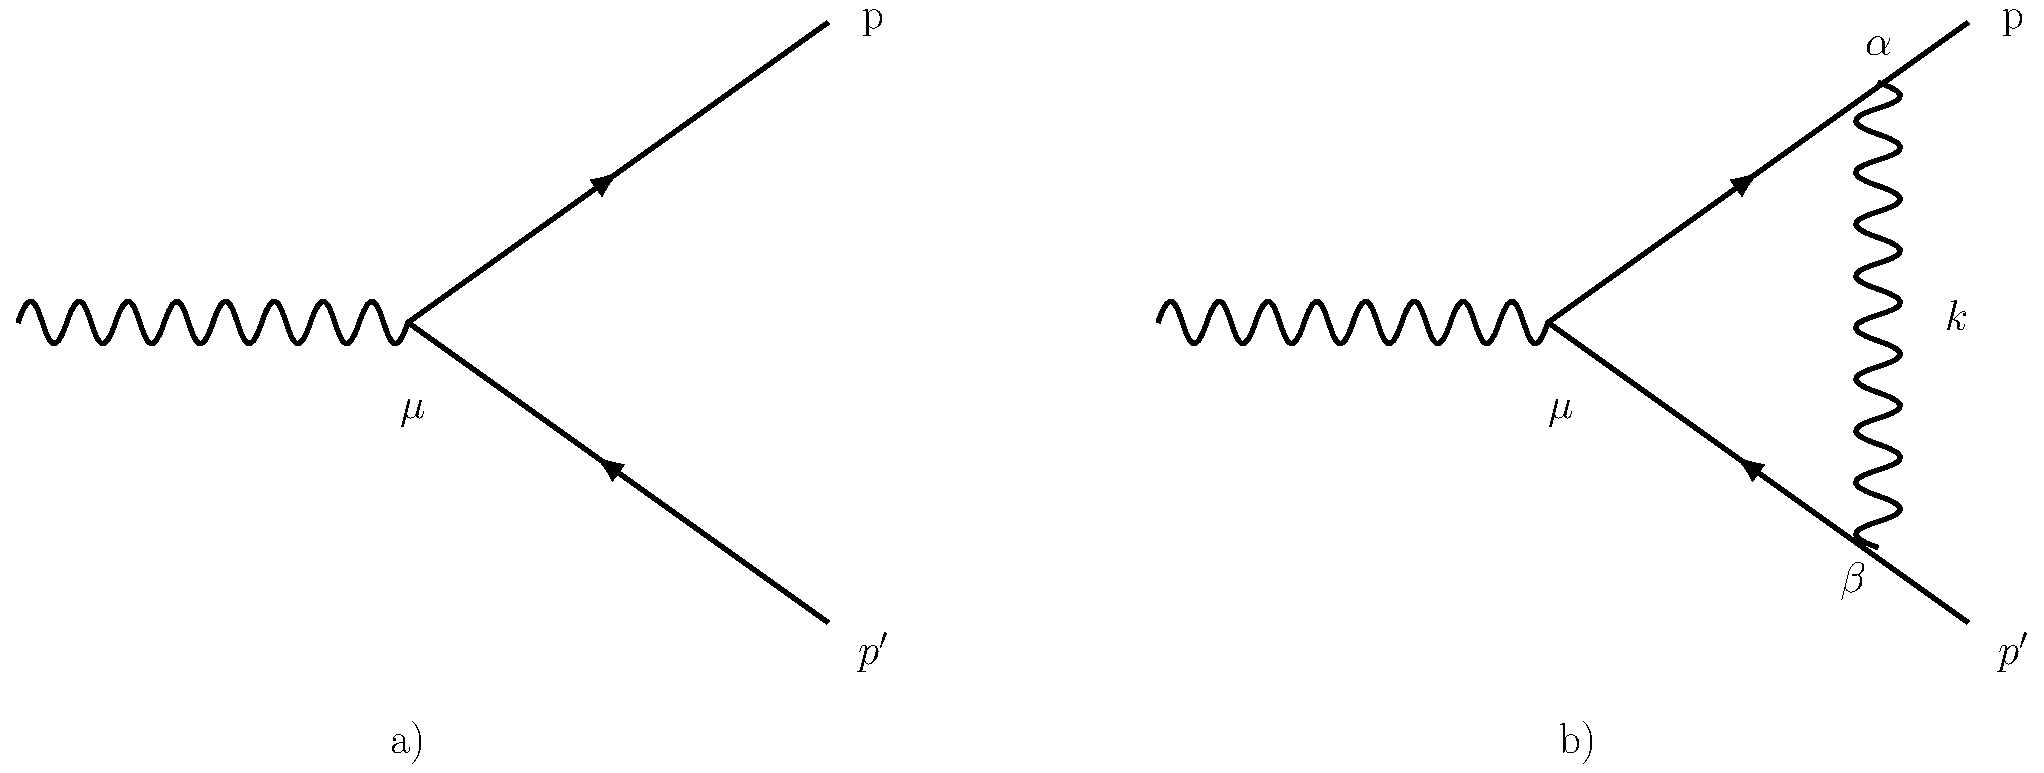
\includegraphics[scale=0.3]{Figures/photonvertexloop.pdf}
    \caption{Leading order and $\mathcal{O}(\alpha)$ correction to virtual photon decay.}
    \label{fig:photon diagrams}
\end{figure}
In this section we will look at the exponentiation of soft photon emission. 
Let us start by considering the amplitude of an off-shell photon decaying to a massless fermion-antifermion pair, see \cref{fig:photon diagrams}. The leading order amplitude is given by
\begin{align}
    \mathcal{M}_{0}=\Bar{u}(p)\gamma^{\mu}v(p')\,,
\end{align}
where coupling factors have been neglected for simplicity. If we now consider the correction, where a photon is emitted from the final state, we get the amplitude
\begin{align}
    \mathcal{M}_{1}=\int\frac{d^{d}k}{(2\pi)^{d}}\Bar{u}(p)\gamma^{\alpha}\frac{(\slashed{p}-\slashed{k})}{(p-k)^{2}}\gamma^{\mu}\frac{(\slashed{k}-\slashed{p'})}{(k-p')^{2}}\gamma^{\beta}v(p')D_{\alpha\beta}(k)\,,
\end{align}
where $D_{\alpha\beta}(k)$ is the photon propagator. 

As we showed in \cref{sec:wilson line properties} the eikonal approximation corresponds to taking the soft limit $k\rightarrow 0$, such that we can neglect $\slashed{k}$ in the numerator and $k^{2}$ in the denominator of the fermion propagators. If we also assume that the fermions are massless, $p^{2}=0$, we get the much simpler eikonal amplitude
\begin{align}\label{eq:factorized eikonal 1 photon amplitude}
    \mathcal{M}_{1}&=\int\frac{d^{d}k}{(2\pi)^{d}}\Bar{u}(p)\gamma^{\alpha}\Big(-\frac{\slashed{p}}{2p\cdot k}\Big)\gamma^{\mu}\Big(\frac{\slashed{p'}}{2p\cdot k}\Big)\gamma^{\beta}v(p')D_{\alpha\beta}(k)\nonumber
    \\
    &=\int\frac{d^{d}k}{(2\pi)^{d}}\big[\bar{u}(p)\gamma^{\mu}v(p'){\big]}\Big(-\frac{p^{\alpha}}{p\cdot k}\Big)\Big(\frac{p'^{\beta}}{p\cdot k}\Big)D_{\alpha\beta}(k)\nonumber
    \\
    &=\mathcal{M}_{0}\int\frac{d^{d}k}{(2\pi)^{d}}\Big(-\frac{p^{\alpha}}{p\cdot k}\Big)\Big(\frac{p'^{\beta}}{p\cdot k}\Big)D_{\alpha\beta}(k)\,,
\end{align}
where we in the second step used the Dirac algebra $\{\gamma^{\mu},\gamma^{\nu}\}=2g^{\mu\nu}$ and the massless Dirac equation, $\bar{u}(p)\slashed{p}=0$ and $\slashed{p'}v(p')=0$. We observe that the tree-level amplitude has been factored out, and contains no divergences. This result is actually an example of factorization of soft physics from hard physics, where the soft part is described by the integral and the hard part is the leading order amplitude $\mathcal{M}_{0}$. The physical reason for this factorization is that the momentum of the soft photon is to low to resolve the inner structure of the hard process. 

Another important observation is that we can define the terms inside the brackets as an eikonal Feynman rule\footnote{This is of course closely related to the Wilson line rules we derived in \cref{sec:wilson line properties}, with the distinction that this is an Abelian theory.}

\begin{fmffile}{ee}
\begin{align}
\begin{gathered}
\begin{fmfgraph*}(45,40)
\fmfleft{i}
\fmfright{o}
\fmf{plain}{i,v3}
\fmf{plain}{v3,o}
\fmffreeze   % freezing the drawn elements
\fmfright{v3,o3}   % adding two more vertices
\fmfforce{(0.5w,0.5h)}{v3}   % setting position of the first vertex
\fmfforce{(0.5w,0h)}{o3}   % setting position of the second vertex
\fmfdot{v3}   % drawing the first vertex with a dot
\fmf{photon, label=$k\downarrow$, l.side=left}{v3,o3}   % drawing a gluon line
\end{fmfgraph*}
\end{gathered}\hspace{0.6cm}&=\frac{p^{\mu}}{p\cdot k}\,.\hspace{2.36cm}\text{Eikonal vertex}\label{eq:Wilson vertex}
\end{align}
\end{fmffile}
This actually means that we can think of the factors multiplying the tree-level amplitude in \cref{eq:factorized eikonal 1 photon amplitude} as a new type of Feynman diagrams, which are \emph{subdiagrams} of the full amplitude. 
\begin{figure}
    \centering
    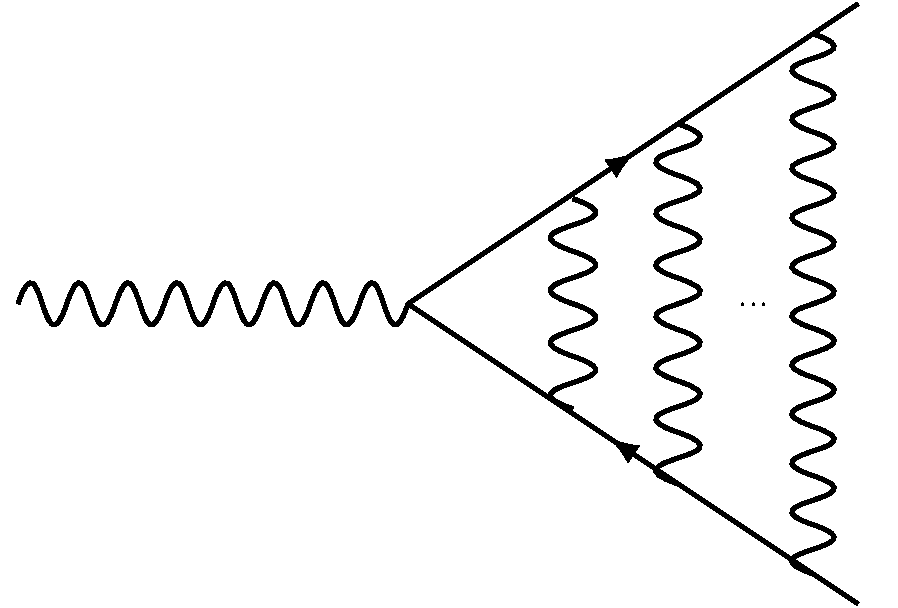
\includegraphics[scale=0.4]{Figures/LadderDiagram.pdf}
    \caption{Ladder diagram of $n$ soft photon emission.}
    \label{fig:Ladder diagram}
\end{figure}

The next step is to generalize to the emission of $n$ soft photons, so let us start with the diagram \cref{fig:Ladder diagram}, where none of the photon lines cross each other, called a \emph{ladder diagram}. This amplitude is given by
\begin{align}\label{eq:nth amplitude}
    \mathcal{M}^{(n)}=\Big(\prod_{i=1}^{n}\int\frac{d^{d}k_i}{(2\pi)^{d}}\Big)\bar{u}(p)\mathcal{E}^{\alpha_1\dots\alpha_n}(p,k_{i})\gamma^{\mu}\mathcal{E}^{\beta_1\dots\beta_n}(p',k_{i})v(p')D_{\alpha_1\beta_1}(k_1)\dots D_{\alpha_n\beta_n}(k_n)\,,
\end{align}
where we have collected the product of fermion propagators and the gamma matrices from the corresponding vertices into $\mathcal{E}$ in the following way
\begin{align}
    \mathcal{E}^{\alpha_1\dots\alpha_n}(p,k_{i})=\frac{\gamma^{\alpha_1}(\slashed{p}-\slashed{k_1})\cdots\gamma^{\alpha_n}(\slashed{p}-\slashed{k_1}- \dots -\slashed{k_n})}{(p-k_1)^{2}\cdots(p-k_1-\dots k_n)^{2}}\,,
\end{align}
and by taking the eikonal approximation this can be simplified to 
\begin{align}
    \mathcal{E}^{\alpha_1\dots\alpha_n}(p,k_{i})=\frac{\bar{u}(p)\gamma^{\alpha_1}\slashed{p}\gamma^{\alpha_2}\slashed{p}\cdots\gamma^{\alpha_n}\slashed{p}}{(-2p\cdot k_1)\cdots (-2p\cdot(k_1+\cdots+k_n)}\,,
\end{align}
which can be further simplified by permuting the gamma matrices using the Dirac algebra and use that $\bar{u}(p)\slashed{p}=0$, giving
\begin{align}
    \bar{u}(p)\mathcal{E}^{\alpha_1\dots\alpha_n}&=\frac{(-1)^{n}\bar{u}(p)p^{\alpha_1}\cdots p^{\alpha_n}}{p\cdot k_1\cdots p\cdot(k_1+\dots +k_n)}\,,
    \\
    \mathcal{E}^{\beta_1\dots\beta_n}v(p')&=\frac{p'^{\beta_1}\cdots p'^{\beta_n}\,v(p')}{p'\cdot k_1\cdots p'\cdot(k_1+\dots +k_n)}\,,
\end{align}
where the factors of $2$ cancels from those in the Dirac algebra, see \cref{eq:Dirac algebra}. 
Combining these two expressions into \cref{eq:nth amplitude}, we get
\begin{align}\label{eq:nth amplitude rewritten}
    \mathcal{M}^{(n)}=\mathcal{M}_{0}\Big(\prod_{i=1}^{n}\int\frac{d^{d}k_i}{(2\pi)^{d}}\Big)\Big[\frac{(-1)^{n}p^{\alpha_1}\cdots p^{\alpha_n}\,p'^{\beta_1}\cdots p'^{\beta_n}\,D_{\alpha_1\beta_1}(k_1)\cdots D_{\alpha_n\beta_n}(k_n)}{p\cdot k_1\cdots p\cdot(k_1+\dots +k_n)\,p'\cdot k_1\cdots p'\cdot(k_1+\dots +k_n)}\Big]\,.
\end{align}

This reveals an intricate dependency on the photon momenta $k_i$, as they are coupled along both the fermion and anti-fermion line. However, we have only considered the ladder diagram where the photons are emitted in the order $k_1\dots k_n$. Therefore, we must sum over all diagrams to this order, meaning we must sum over all permutations of the emitted photon momenta. We start by fixing the order of photon emission on the anti-fermion line, and sum over permutations on the fermion line. If we let $\pi$ denote a permutation of $(1,2,\dots,n)$, which maps to $(\pi_1,\pi_2,\dots \pi_n)$, the sum over diagrams correspond to making the following substitution
\begin{align*}
    \frac{1}{p\cdot k_1\cdots p\cdot(k_1+\dots +k_n)}\rightarrow \sum_{\pi}\frac{1}{p\cdot k_{\pi_1}\cdots p\cdot(k_{\pi_1}+\dots +k_{\pi_n})}\,.
\end{align*}
Then we can make use of the so-called \emph{eikonal identity}\footnote{This identity can be proven by using the Wilson lines we considered in \cref{sec:wilson line properties}, but for a standard derivation we refer the reader to \cite{Peskin:257493}.}
\begin{align}
    \sum_{\pi}\frac{1}{p\cdot k_{\pi_1}\cdots p\cdot(k_{\pi_1}+\dots +k_{\pi_n})}=\prod_{i=1}^{n}\frac{1}{p\cdot k_i}\,.
\end{align}
If this seems mysterious, let us show a simple example that highlights how this works. For the simple case of $n=2$, we have that
\begin{align}
    \frac{1}{p\cdot k_1\,p\cdot(k_1+k_2)}+\frac{1}{p\cdot k_2\,p\cdot(k_1+k_2)}=\frac{1}{p\cdot k_1\,p\cdot k_2}\,,
\end{align}
which shows the structure.

So by using the eikonal identity we substantially simplify the dependence on the photon momenta for the fermion line, as they have decoupled from each other. We could hope to do the same on the anti-fermion line, but that is not possible as they have already been fixed. However, we can exploit that $k_i$ are dummy variables inside the integral. The integrand has a symmetric Lorentz structure under the permutation of any two momenta, which means that we can make the replacement
\begin{align}
    \Big(&\prod_{i=1}^{n}\int\frac{d^{d}k_i}{(2\pi)^{d}}\Big)\frac{1}{p'\cdot k_1\cdots p'\cdot(k_1+\dots +k_n)}\nonumber
    \\
    &=\frac{1}{n!}\Big(\prod_{i=1}^{n}\int\frac{d^{d}k_i}{(2\pi)^{d}}\Big)\sum_{\pi}\frac{1}{p'\cdot k_{\pi_1}\cdots p'\cdot(k_{\pi_1}+\dots +k_{\pi_n})}\nonumber
    \\
    &=\frac{1}{n!}\prod_{i=1}^{n}\int\frac{d^{d}k_i}{(2\pi)^{d}}\frac{1}{p'\cdot k_i}\,,
\end{align}
where we have used that there are $n!$ such permutations. 

Substituting these simplifications into \cref{eq:nth amplitude rewritten}, we get
\begin{align}
    \mathcal{M}^{(n)}&=\mathcal{M}_{0}\frac{1}{n!}\prod_{i=1}^{n}\int\frac{d^{d}k_i}{(2\pi)^{d}}\big(\frac{p^{\alpha_i}}{p\cdot k_i}\big)\big(\frac{-p'^{\beta_i}}{p'\cdot k_i}\big)D_{\alpha_i\beta_i}(k_i)\nonumber
    \\
    &=\mathcal{M}_{0}\frac{1}{n!}\Big[\int\frac{d^{d}k}{(2\pi)^{d}}\big(\frac{p^{\alpha}}{p\cdot k}\big)\big(\frac{-p'^{\beta}}{p'\cdot k}\big)D_{\alpha\beta}(k)\Big]^{n}\,.
\end{align}
This looks very much like the $n$th term in a Taylor expansion of an exponential. By using the eikonal approximation we have found the remarkable result that the sum over all $n$ photon graphs is given by the one-loop graph to the $n$th power! If we take the sum over all diagrams for any number of single soft photon emission, we find the all order amplitude
\begin{align}\label{eq:exponentiated amplitude}
    \mathcal{M}&=\sum_{n=1}^{\infty}\mathcal{M}^{(n)}=\mathcal{M}_{0}\exp\Big(\int\frac{d^{d}k}{(2\pi)^{d}}\big(\frac{p^{\alpha}}{p\cdot k}\big)\big(\frac{-p'^{\beta}}{p'\cdot k}\big)D_{\alpha\beta}(k)\Big)\,,
\end{align}
which demonstrates that the hard part factorizes from the soft part also in the all order case, with the addition that the soft part exponentiates. From the structure of \cref{eq:exponentiated amplitude}, we can write the amplitude on the factorized form
\begin{align}
    \mathcal{M}=\mathcal{H}\mathcal{S}\,,
\end{align}
where $\mathcal{H}$ is a hard scattering function and $\mathcal{S}$ is a soft scattering function. The hard function is finite, while the soft function contains all the soft and collinear divergences. It is important to note that we have only considered single photon emissions, but to be general one should in fact consider the case where the emitted photons could connect off the external lines, via fermion loops. This would extend the result in \cref{eq:exponentiated amplitude} to include the sum over all connected diagrams including loops in the exponent, see \cite{1961AnPhy..13..379Y}. 

As already mentioned the complexity increases substantially for a non-abelian gauge theory, and while the result has existed in literature for a long time \cite{Gatheral:1983cz,Frenkel:1984pz}, the proof is restricted to involve only two coloured external particles. This proof covers Drell-Yan like processes, but if the final state contains coloured particles as well this proof does not hold. This scenario has been studied in great detail and recent work has been done to improve it to include several coloured particles \cite{White:2015wha,Laenen:2008gt}. The proof is too advanced to go into detail on here, but the main idea is to use a path integral approach with Wilson lines as a source for creating particles from the vacuum. From there one uses the so-called replica method from statistical mechanics to show that the theory can be written as $N$ replicas leading to the structure of webs.



% %\section{Threshold Factorization}
In \cref{sec:Drell-Yan Hadronic Cross Section} we used the QCD factorization theorem and wrote the hadronic Drell-Yan cross section on the form\footnote{The difference here is that we have not factored out the Born cross section at this point.}
\begin{align}\label{eq:resummation factorized drell-yan Cross Section}
   \frac{ d\sigma_{h_1h_2}}{dQ^{2}}=\sum_{i,j}\int dx_{1}dx_{2}\,f_{i/h_1}(x_1,\mu)f_{j/h_2}(x_2,\mu)\,\hat{\sigma}_{ij}\Big(z,Q,\mu,\alpha_s(\mu^{2})\Big)\,.
\end{align}
As we have said many times before, these parton distribution functions $f_{i/h_{1}}$ are not perturbative and have to be extracted from experiment. We made an $\mathcal{O}(\alpha_s)$ calculation of the hard partonic cross section in \cref{sec:Drell-Yan Hadronic Cross Section}, where we found both collinear and soft divergences. By summing over all diagrams we found that some of these canceled, and the last divergence were treated by considering a refactorization using parton-in-parton distributions. However, the final result contained terms that give large logarithmic corrections near threshold. The way to treat these large logarithms is by using the non-Abelian eikonal exponentiation theorem, see (\ar{ref to nonA exponentiation}). 

Let us first consider the partonic equivalent to \cref{eq:resummation factorized drell-yan Cross Section} using parton-in-parton distributions
\begin{align}
    \frac{d\hat{\sigma}_{ij}}{dQ^{2}}=\sum_{kl}\int dy_{1}dy_{2}f_{k/j}(x_1,\mu)f_{l/j}(x_2,\mu)\,\hat{\sigma}_{kl}(z,Q,\mu,\alpha_s(\mu^{2}))\,
\end{align}

%%%%%%%%%%%%%%%%%%%%%%%%%%%%%%%%%%%%%%%%%%%%%%%%%%%%%%%%%%%%
\section{Hadronic Cross Section and Inverse Mellin}
In this section we will recover the hadronic cross section in Drell-Yan $x$-space, and discuss how we can evaluate the inverse Mellin transform. 

From \cref{eq:hadronic cross section in Mellin} and \cref{eq:LL result} the Mellin transformed hadronic cross section is given by \footnote{We have set $\mu=Q$, and for generality inserted the hard function $H_{ij}$.}
\begin{align}
    \tilde{\sigma}_{h_1h_2}(N)&=\int_{0}^{1}d\tau \tau^{N-1}\,\frac{1}{\sigma_{0}}\frac{d\sigma_{h_1h_2}}{dQ^{2}}\nonumber
    \\
    &=\sum_{i,j=q,\bar{q}}H_{ij}\big((Q,\alpha_{s}(Q)\big)\tilde{f}_{i/h_1}(N,Q)\tilde{f}_{j/h_2}(N,Q)\,\exp\big(\Me{E}_{ij}(N,Q,\alpha_s)\big)
\end{align}
where the hard function has been exponentiated. We can now use the inverse Mellin transform \cref{eq:Appendix Inverse Mellin} to write\footnote{We recover the fractional charge of the quarks.}
\begin{align}
    \frac{d\sigma_{h_1h_2}}{dQ^{2}}=&\,\sigma_{0}\sum_{i,j=q,\bar{q}}Q_{q}^{2}H_{ij}\big((Q,\alpha_{s}(Q)\big)\nonumber
    \\
    &\frac{1}{2\pi i}\int_{c-i\infty}^{c+i\infty}dN\,\tau^{-N}\tilde{f}_{i/h_1}(N,Q)\tilde{f}_{j/h_2}(N,Q)\exp\big(\Me{E}_{ij}(N,Q,\alpha_s)\big)
\end{align}

There exists numerical packages to evaluate parton distributions in Mellin space, see \cite{Vogt_2005}. However, to use the $x$-space formalism we can do several manipulations by using the convolution properties of the Mellin transform.


\subsection{The Inverse Mellin Transform}
The inverse Mellin transform as defined in \cref{sec:Appendix Mellin Transform}, is for a general function given by
\begin{align}\label{eq:h}
    h(x)=\frac{1}{2\pi i}\int_{c-i\infty}^{c+i\infty}dN\,x^{-N}\,\Me{h}(N)
\end{align}
where 
\begin{align*}
    \Me{h}(N)=\int_{0}^{\infty}dx\,x^{N-1}\,h(x)
\end{align*}
since $h(x)$ is a real valued function
\begin{align}\label{eq:h_real}
    \Me{h}^{*}(N)=\int_{0}^{\infty}dx\,x^{N^{*}-1}\,h(x)=\Me{h}(N^{*})
\end{align}
The Mellin inversion integral \cref{eq:h} can be splitted into two, one part for the lower bound and one part for the upper bound. In the lower bound term a change of variable will be made $N\rightarrow N^{*}$, which makes the integration bounds change accordingly $c-i\infty\rightarrow c+i\infty$.
\begin{align}
    h(x)&=\frac{1}{2\pi i}\Bigl(\int_{c-i\infty}^{c}dN\,x^{-N}\,\Me{h}(N)+\int_{c}^{c+i\infty}dN\,x^{-N}\,\Me{h}(N)\Bigr)\nonumber
    \\
    &=\frac{1}{2\pi i}\Bigl(\int_{c+i\infty}^{c}dN^{*}\,x^{-N^{*}}\,\Me{h}(N^{*})+\int_{c}^{c+i\infty}dN\,x^{-N}\,\Me{h}(N)\Bigr)\nonumber
    \\
    &=\frac{1}{2\pi i}\Bigl(-\int_{c}^{c+i\infty}dN^{*}\,x^{-N^{*}}\,\Me{h}^{*}(N)+\int_{c}^{c+i\infty}dN\,x^{-N}\,\Me{h}(N)\Bigr)\,,
    \intertext{and by choosing the parametrization of the Mellin variable to be $N=c+ze^{i\phi}$, with $z$ real, the integral will take the form}
    &=\frac{1}{2\pi i}\int_{0}^{\infty}dz\,\left(e^{i\phi}\,x^{-N}\Me{h}(N)-e^{-i\phi}\,x^{-N^{*}}\Me{h}^{*}(N)\right)\nonumber
    \\
    &=\frac{1}{2\pi i}\int_{0}^{\infty}dz\,2i\,\text{Im}\left(e^{i\phi}\,x^{-N}\Me{h}(N)\right)\nonumber
    \\
    &=\frac{1}{\pi}\int_{0}^{\infty}dz\,\text{Im}\left(e^{i\phi}\,x^{-N}\Me{h}(N)\right)\,,
\end{align}
where the relation used in the third last step is
\begin{align*}
    \Me{h}(N)-\Me{h}^{*}(N)&=2i\,\text{Im}(\Me{h}(N))\,.
\end{align*}
Writing out the parametrization, the integral is equal to
\begin{align}\label{eq:Inversed Mellin Integral}
    h(x)=\frac{1}{\pi}\int_{0}^{\infty}dz\,\text{Im}\left(e^{i\phi}\,x^{-c-z\,\exp(i\phi)}\Me{h}(c+z\,\exp(i\phi))\right)\,.
\end{align} 
% \section{Mellin Space Factorization}\label{sec:Resummation Drell-yan}
In the NLO calculation \cref{sec:renormalizing drell-yan}, we found that the final hard scattering function was infrared safe. However, in the cancellation of infrared divergences, we found the emergence of logarithmic distributions. These logarithmic distributions appear at every order and ruin the convergence of the perturbative expansion in the threshold regime. To handle these large corrections, we have to use threshold resummation techniques. Threshold resummation was first derived for the Drell-Yan process \cite{Sterman:1986aj,CATANI1989}. These papers laid the groundwork for resummation of large contributions in many hard QCD processes. 

\subsection{Phase Space Factorization}
A fundamental ingredient for resummation in QCD, is that the eikonal approximation leads to exponentiation. Near the threshold, most of the available energy goes to producing the final state particles. Therefore, the emitted gluons are soft, and the eikonal approximation corresponds to taking the partonic threshold limit. However, the derivation of eikonal exponentiation in \cref{sec:Eikonal} was at the level of amplitudes. Eventually, we want the full cross-section to exponentiate, including the underlying hard process. The problem is that the hard part contains phase space integrals, which may lead to an intricate dependency between the final state gluon momenta. If the cross-section is to exponentiate the gluon momenta must disentangle from each other. To make this problem explicit, let us consider the Drell-Yan process where the differential phase space for the emission of $n$ soft gluons can be written as
\begin{align}
    d\mathcal{P}^{(n)}&=\frac{d^{4}q}{(2\pi)^{4}}\,\prod_{i=1}^{n}\frac{d^{3}k_{i}}{(2\pi)^{3}}\frac{1}{2k_{i}^{0}}\,2\pi\delta^{+}(q^{2}-Q^{2})(2\pi)^{4}\delta^{(4)}\Big(p_1+p_2-q-\sum_{i}k_i\Big)\nonumber
    \\
    &=\prod_{i=1}^{n}\frac{d^{3}k_{i}}{(2\pi)^{2}}\frac{1}{2k_{i}^{0}}\,\delta\Big(\Big[p_1+p_2-\sum_{i}k_i\Big]^{2}-Q^{2}\Big)\,,
\end{align}
where we began with the general expression for clarity and applied the delta function. Here $k_i$ is the gluon momenta, $q$ is the photon momenta, $p_1$ and $p_2$ is the incoming quarks and $Q^{2}$ is the final state invariant mass. In the soft gluon region we can make the approximation 
\begin{align}\label{eq:n-phase space exponentiation}
    d\mathcal{P}^{(n)}&\approx\prod_{i=1}^{n}\frac{d^{3}k_{i}}{(2\pi)^{2}}\frac{1}{2k_{i}^{0}}\delta\Big(\hat{s}-2\sum_{i}k_{i}^{0}\sqrt{\hat{s}}-Q^{2}\Big)\nonumber
    \\
    &=\prod_{i=1}^{n}\frac{d^{3}k_{i}}{(2\pi)^{2}}\frac{1}{2k_{i}^{0}}\frac{1}{\hat{s}}\delta\Big(1-z-\sum_i \omega_{k_i}\Big)\,,
\end{align}
where we have defined the fractional energy of the $i$th gluon as $\omega_{k_i}=2k_i^{0}/\sqrt{\hat{s}}$, and $z$ is the usual partonic threshold variable, $z=Q^{2}/\hat{s}$. We observe that the delta function forces the emitted gluon momenta to depend on each other, spoiling the factorization of the phase space.

There is a neat solution to this problem via the Laplace transform. In general, the Laplace transform of a delta function is given by
\begin{align}
    \mathcal{L}[\delta(x-y)](N)=e^{-Ny}\,.
\end{align}
where $N\in\mathbb{C}$. The goal now is to try to disentagle the delta function, so if we take the inverse Laplace of the delta function in \cref{eq:n-phase space exponentiation} we obtain the expression
\begin{align}\label{eq:inverse Laplace}
    \delta(1-z-\sum_i \omega_{k_i})=\frac{1}{2\pi i}\int_{c-i\infty}^{c+i\infty}dN\, e^{N(1-z-\sum_i \omega_{k_i})}\,.
\end{align}
However, we are only interested in the threshold regime $z\rightarrow 1$, so let us consider the following Taylor series
\begin{align}
    \ln z=\sum_{n=1}^{\infty}(-1)^{n}\frac{(1-z)^{n}}{n}\,,
\end{align}
leading to the approximate identity, $e^{N(1-z)}\approx e^{-N\ln z}=z^{-N}$. With this approximation \cref{eq:inverse Laplace} takes the form
\begin{align}
    \delta(1-z-\sum_i \omega_{k_i})=\frac{1}{2\pi i}\int_{c-i\infty}^{c+i\infty}dN\, z^{-N}\prod_{i=1}^{n}e^{-N\omega_{k_i}}\,,
\end{align}
which is an inverse Mellin transform, see \cref{sec:Appendix Mellin Transform}. The consequence of this result is made clear if we take the Mellin transform of the differential phase space
\begin{align}
    \int_{0}^{1}dz\,z^{N-1}\,d\mathcal{P}_{n}=\prod_{i=1}^{n}\frac{d^{3}k_{i}}{(2\pi)^{2}}\frac{1}{2k_{i}^{0}}\frac{1}{\hat{s}}e^{-N\omega_{k_i}}\,,
\end{align}
giving that the phase space has taken a factorized form, enabling it to exponentiate.

\subsection{Hadronic Cross Section in Mellin Space}
Factorization of the phase space is not the only advantage of using the Mellin transform. In \cref{sec:Drell-Yan Hadronic Cross Section}, we wrote the factorized Drell-Yan cross section as
\begin{align}\label{eq:Factorized Dre-Yan Cross Section}
   \frac{ d\sigma_{h_1h_2}}{dQ^{2}}=\sigma_{0}\sum_{i,j}\int \frac{dx_{1}}{x_1}\frac{dx_{2}}{x_2}f_{i/h_1}(x_1,\mu)f_{j/h_2}(x_2,\mu)\,\omega_{ij}\Big(z,Q,\mu,\alpha_s(\mu^{2})\Big)\,.
\end{align}

Instead of working with the convoluted integrals, we consider the Mellin transform in the hadronic threshold variable $\tau=x_1x_2z$. In this expression it is only the hard function that is calculable in perturbation theory and is the main function of interest. Hence, let us divide out the Born cross section and define the Mellin space hadronic cross section\footnote{We will recover the Born cross section when we return to the resummed hadronic cross section. We have also neglected the fractional charge of the quarks for simplicity.} 
\begin{align}\label{eq:hadronic cross section in Mellin}
    \tilde{\sigma}_{h_1h_2}(N)&=\int_{0}^{1}d\tau \tau^{N-1}\,\frac{1}{\sigma_{0}}\frac{d\sigma_{h_1h_2}}{dQ^{2}}\nonumber
    \\
    &=\sum_{i,j}\tilde{f}_{i/h_1}(N,\mu)\tilde{f}_{j/h_2}(N,\mu)\,\tilde{\omega}_{ij}\Big(N,Q,\mu,\alpha_s(\mu^{2})\Big)\,,
\end{align}
where
\begin{align}
    \tilde{\omega}_{ij}(N)=\int_{0}^{1}dz\,z^{N-1}\,\omega_{ij}(z)\,,
    \\
    \tilde{f}_{i/h_1}(N)=\int_{0}^{1}dx\,x^{N-1}\,f_{i/h_1}(x)\,.
\end{align}
Here we observe that one of the advantages of working in Mellin space is that the convolution has turned into simple products. If this transformation seems obscure, see \cref{eq:Appendix Mellin convolution transform}.

To see how the threshold logarithms manifest themselves in Mellin space, we take the limit $z\rightarrow 1$ of \cref{eq:NLO drell yan hard function}, giving
\begin{align}
    \omega_{q\bar{q}}=\delta(1-z)+\frac{\alpha_s}{\pi}C_{F}\Big(4\Big[\frac{\ln(1-z)}{1-z}\Big]_{+}+\Big(\frac{\pi^{2}}{3}-4\Big)\delta(1-z)\Big)+\mathcal{O}(\alpha_{s}^{2})\,.
\end{align}
By using the Mellin transforms given in \cref{sec:Appendix Mellin Transform}, we find the Mellin space expression
\begin{align}\label{eq:Mellin space NLO of omegaqbarq}
    \Me{\omega}_{q\bar{q}}=1+\frac{\alpha_s}{\pi}C_{F}2\ln^{2}\bar{N}+\mathcal{O}(\alpha_{s}^{2})\,,
\end{align}
where $\bar{N}=Ne^{\gamma_{E}}$, and we omitted constant terms that has no relevance compared to the logarithm. We observe that the threshold limit $z\rightarrow 1$, corresponds to $N\rightarrow\infty$. Hence, the constant factors are unimportant for large $N$. 

To $n$-th power of the logarithm, we have that the plus distributions give terms of the form
\begin{align}
    \int_{0}^{1}dz z^{N-1}\Big[\frac{\ln^{n}(1-z)}{(1-z)}\Big]_{+}=\frac{(-1)^{n+1}}{n+1}\ln^{n+1}(\bar{N})+\mathcal{O}(\ln^{n-1}(\bar{N}))\,,
\end{align}
after Mellin transformation. These are the logarithms we now want to resum, and try to reproduce after the resummation procedure has been performed. In order to make progress, we will use the factorization property of QCD to refactorize the cross section by using parton-in-parton distributions. We also used this property in the fixed order Drell-Yan calculation, where we had that the hard function $\omega_{ij}$ were collinear divergent. By refactorizing the hard functions by using parton-in-parton distributions we showed that the hard function could be rendered infrared safe as the parton-in-parton distributions were responsible for these. This is a very important feature that we will exploit heavily in the sections to come. 

\subsection*{Kinematics}
Let us briefly look at some of the kinematics that is used. We choose the quarks to be fully collinear to the incoming protons, i.e.
\begin{align}
    p_{1}&=x_{1}P_1\,,
    \\
    p_{2}&=x_{2}P_2\,.
\end{align}
We work in the centre of mass frame of $P_1$ and $P_2$, with $P_{1}^{0}=P_{2}^{0}=E=Q/2$. The hadrons have the following momenta
\begin{align}
    P_{1}&=\frac{Q}{2}(1,1,0)
    \\
    P_{2}&=\frac{Q}{2}(1,-1,0)\,,
\end{align}
such that
\begin{align}
    s=(P_1+P_2)^{2}=Q^{2}\,.
\end{align}
In the threshold limit $\tau\rightarrow 1$, we have that $\tau$ coincides with $z$ when $x_{1}\rightarrow 1$ and $x_{2}\rightarrow 1$. Hence, we have that the momenta of the quarks are $p_1=P_1$ and $p_2=P_2$. Also, if a gluon radiates from an incoming quark, it follows that the energy of that gluon is given by
\begin{align}
    Q^{2}&=(p_1+p_2-k)^{2}=s-2\sqrt{s}k^{0}
    \\
    &\rightarrow k^{0}=(1-\tau)Q/2\,.
\end{align}

\newpage
\section{Threshold Factorization}\label{sec:threshold factorization}
In this section we will use factorization theorems to find a fully factorized form of the hard function $\Me{w}_{ij}(N)$. 

First we want to extract the universal collinear singularities we encountered in the fixed order NLO calculation. We do the same as in \cref{sec:renormalizing drell-yan} and define a partonic analogue to the hadronic cross section \cref{eq:hadronic cross section in Mellin},
\begin{align}\label{eq:partonic analogue to hadronic in mellin }
    \tilde{\sigma}_{ij}(N)=\tilde{f}_{i/i}(N,\mu,\epsilon)\tilde{f}_{j/j}(N,\mu,\epsilon)\,\Me{\omega}_{ij}(N,Q,\mu,\alpha_{s})\,,
\end{align}
where $f_{i/i}$ are the light-cone distributions responsible for the collinear singularities. Thus, the partonic function $\Me{\omega}_{ij}$ is with this refactorization infrared safe.  
%\begin{align}
%    \frac{d\Me{\sigma}_{ij}}{dQ^{2}}(w,\epsilon)&=\sigma_{0}H_{ij}(\alpha_{s}(Q))\int \frac{dx_{1}}{x_1}\frac{dx_{2}}{x_2}dw_s\,J_{i/i}(x_1,Q,\epsilon)J_{j/j}(x_2,Q,\epsilon)\,S_{ij}(w_s,Q)\nonumber
%    \\
%    &\hspace{2cm}\delta(1-\tau-(1-x_1)-(1-x_2)-w_s)\,.
%\end{align}
%We define $w=1-\tau$, $w_1=1-x_1$, $w_2=1-x_2$ and $w_s=2\sum_{i}k_{i}^{0}/Q$, where $\sum_{i}k_{i}^{0}$ is total the energy of the emitted gluons. We call these weights, and they become small in the threshold region. The delta function result from taking the threshold limit of $\delta(Q^{2}-(p_{1}^{\mu}+p_{2}^{\mu}-\sum_{i}k_{i}^{\mu})^{2})$, taking only linear terms of $w_{i}$ into account. This is needed as we want the collinear and soft divergences to decouple, so we demand that all the weights are independent and additive, i.e. $w=w_1+w_2+w_s$\footnote{For more detail on near threshold factorization, see \cite{Sterman:1986aj,Kidonakis:1997gm,Contopanagos:1996nh}.}.
We can go even further with the factorization theorem. 

As we saw in \cref{sec:NLO drell yan calculation}, the cancellation of soft divergences are responsible for the large logarithms. Hence, we want to factorize out these soft parts and use the non-Abelian eikonal exponentiation theorem to resum them. We begin with defining a threshold analogue to \cref{eq:hadronic cross section in Mellin}  \cite{Sterman:1986aj}
\begin{align}\label{eq:threshold factorization Mellin}
    \Me\sigma_{ij}(N)&=H_{ij}(Q,\alpha_{s}(Q))\Me{J}_{i/i}(N,Q,\epsilon)\Me{J}_{j/j}(N,Q,\epsilon)\Me{S}_{ij}(N,Q,\mu,\alpha_{s}(\mu))\,,
\end{align}
where $H_{ij}(Q)$ is a hard function that is free of singular distributions. We have also defined jet functions $J_{i/i}(N)$. We specifically defined these as functions of $Q$ and not $\mu$, which we will comment on later. These contain additional collinear divergences, that will cancel the collinear singularities contained in the light-cone distributions $f_{i/i}(x,\mu,\epsilon)$. Lastly, we have a soft function $S_{ij}(N)$ that is responsible for all wide angle soft radiation. The derivation of this formula is quite technical, but we will try to give the main arguments behind it\footnote{For a more comprehensive explanation, see \cite{Collins:1989gx}.}.
\begin{figure}
    \centering
    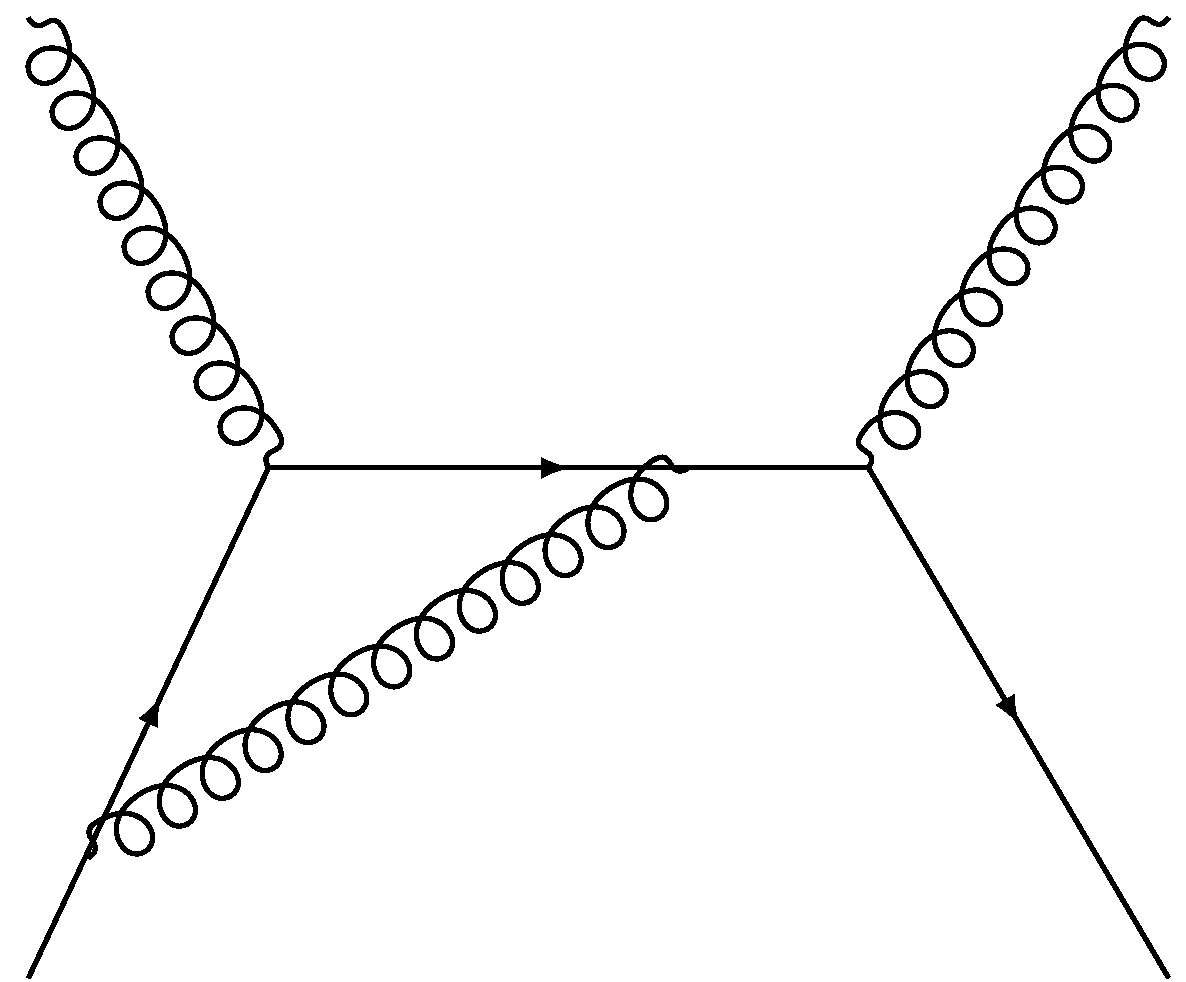
\includegraphics[scale=0.2]{Figures/An Example Diagram.pdf}
    \caption{Diagram that has no IR-divergences.}
    \label{fig:Gluon connected to propagator}
\end{figure}

The first step is to decouple $H$ from $S$. Diagrams such as \cref{fig:Gluon connected to propagator} does not generate IR-divergences. This is true to all order, i.e. a soft line can only generate an IR divergence if it is connected to an on-shell external line \cite{sterman_1993}. Thus, gluons that connect the soft and the hard part do not contribute to the IR-divergences, i.e. the soft and hard part cannot be connected directly. The physical interpretation of such a decoupling is that soft gluons correspond to large length scales, while the hard part takes place at small length scales. Therefore the soft gluons are unable to resolve the internal structure of the hard process. This fact also follows from the eikonal approximation we made in \cref{sec:wilson line properties}, where we showed that the eikonal approximation led to the concept of particles dressed with Wilson lines. This was only possible if the soft emission was connected to an on-shell external line.

The second step of the argument is to decouple the jets from each other. By definition all jets move in different directions, so lines in different jets are proportional to different momenta. We have two jets that meet at the hard interaction, but before that they cannot combine. Thus their collinear divergences will not mix with each other \cite{Sterman78}. Again, based on length scales the small momentum of the gluons in the $J_i$ cannot resolve the inner structure of the hard process. The decoupling of the jets from the soft part is more subtle, but since jets have large total momentum their substructure cannot be resolved by the soft gluons in $S$. However, close to the threshold there are energy restrictions on the gluons, leading to the large logarithmic corrections. Hence, the soft function does not completely decouple and we have to take it into account. This soft function can be constructed by taking the eikonal approximation of the partonic process, i.e. we can build it out of Wilson lines. We will come back to this procedure in the next section.

Close to the threshold we have that \cref{eq:partonic analogue to hadronic in mellin } and \cref{eq:threshold factorization Mellin} must be equal, giving the fully factorized hard function
\begin{align}\label{eq:partonic hard function ratio in mellin}
    \Me{\omega}_{ij}(N,Q,\mu,\alpha_s(\mu))=\frac{\Me{J}_{i/i}(N,Q,\epsilon)\Me{J}_{j/j}(N,Q,\epsilon)}{\tilde{f}_{i/i}(N,\mu,\epsilon)\tilde{f}_{j/j}(N,\mu,\epsilon)}H_{ij}(Q,\alpha_{s}(\mu))\Me{S}_{ij}(N,Q,\mu,\alpha_{s}(\mu))\,.
\end{align}

Since the partonic function is defined to be infrared safe, the ratio of the jet and parton distributions must cancel the collinear divergences. The ratio of distributions might seem strange and it may not be obvious at this point how to evaluate them. But we will show later how this is done using renormalization group equations. 

The next step going forward is to make use of what we know of Wilson lines in order to construct the soft function. We will do this by constructing an eikonal cross section, i.e. a cross section where the radiation is restricted to be soft. Then we will show that the soft function can be replaced from \cref{eq:partonic hard function ratio in mellin} by the eikonal cross section. The motivation behind this is to use the non-Abelian eikonal exponentiation theorem to calculate the eikonal cross section.  


































  
% \section{Factorization of Soft Gluons}\label{sec:factorization soft gluons}
In this section we will take a closer look at how we can organize the soft contributions coming from $\tilde{S}$ by constructing the eikonal cross section.

Near threshold all radiation is restricted to be soft compared with the hard scattering function. This naturally leads to an eikonal approximation for the cross section, i.e. we can construct this cross section by using Wilson lines. To this end, we consider the following Wilson lines\footnote{This definition is slightly different in appearance to the ones we derived in \cref{sec:wilson line properties}, but all the rules are equivalent.}
\begin{align}
    \mathcal{U}_{p}[x,\infty]=\mathcal{P}\exp{ig\int_{\infty}^{0}ds\,p\cdot A(x+ps)}\,,
    \\
    \mathcal{U}_{-p}[\infty,x]=\mathcal{P}\exp{-ig\int_{0}^{\infty}ds\,p\cdot A(x-ps)}\,,
\end{align}
where we have parametrized the path as $z^{\mu}=x^{\mu}+p^{\mu}s$, where $p$ is the light-like momentum of the incoming massless quark (or anti-quark) and $s$ is the proper time. From this we can construct the Drell-Yan Wilson line\footnote{If the notation $\mathcal{U}(0)$ is confusing it just mean that the composition are connected such that the two Wilson lines meet at space-time point 0.}
\begin{align}
    \mathcal{U}_{DY}(0)=\mathcal{U}_{-p_2}[\infty,0]\,\mathcal{U}_{p_1}[0,\infty]\,,
\end{align}
where $\mathcal{U}_{p_1}[\infty,0]$ and $\mathcal{U}_{-p_2}[\infty,0]$ are the Wilson lines evaluated along the classical trajectories of the incoming massless quark and anti-quark. The classical trajectory means that the particles are so energetic that they will not recoil as the soft gluons are emitted, such that they move along a straight line. This is necessary as we want to use Wilson lines on linear paths. From this we can construct the expectation value\footnote{There is an implicit average and sum over colour in this expectation value.}
\begin{align}\label{eq:1st DY wilson loop}
    \mathcal{W}_{DY}(0)=\bra{0}\Bar{\mathcal{T}}\,\mathcal{U}_{DY}^{\dagger}(0)\mathcal{T}\,\mathcal{U}_{DY}(0)\ket{0}\,,
\end{align}
where $\mathcal{T}$ and $\Bar{\mathcal{T}}$ are the time and anti-time ordering operators. 

The main idea from here is to construct a Wilson loop expectation value. To this end, we rewrite \cref{eq:1st DY wilson loop} by inserting a complete set of final states
\begin{align}
    \mathcal{W}_{DY}(0)=\sum_{n}\bra{0}\Bar{\mathcal{T}}\,\mathcal{U}_{DY}^{\dagger}(0)\ket{n}\bra{n}\mathcal{T}\,\mathcal{U}_{DY}(0)\ket{0}\,,
\end{align}
and the eikonal cross section is then constructed by inserting a energy conserving delta function, i.e.
\begin{align}
    \sigma_{ij}^{(\text{eik})}(\tau,Q)=\sum_{n}\delta((1-\tau)Q/2-E_{n})\bra{0}\Bar{\mathcal{T}}\,\mathcal{U}_{DY}^{\dagger}(0)\ket{n}\bra{n}\mathcal{T}\,\mathcal{U}_{DY}(0)\ket{0}\,,
\end{align}
where $E_{n}=\sum_{n}k_{n}^{0}$ is the total energy of the emitted gluons, which is restricted to be $(1-\tau)Q/2$. 

By using the Fourier representation of the delta function, we find
\begin{align}\label{eq:eikonal cross section wilson loop}
    \sigma_{ij}^{(\text{eik})}(\tau,Q,\mu,\alpha_s,\epsilon)&=\frac{Q}{2}\sum_{n}\int_{-\infty}^{\infty}\frac{dy^{0}}{2\pi}\,e^{iy^{0}((1-\tau)Q/2-\sum_{n}k_{n}^{0})}\bra{0}\Bar{\mathcal{T}}\,\mathcal{U}_{DY}^{\dagger}(0)\ket{n}\bra{n}\mathcal{T}\,\mathcal{U}_{DY}(0)\ket{0}\nonumber
    \\
    &=\frac{Q}{2}\int_{-\infty}^{\infty}\frac{dy^{0}}{2\pi}\,e^{iy^{0}(1-\tau)Q/2}\,\mathcal{W}_{DY}(y)\,,
\end{align}
where we have explicitly included the dimensional regulator $\epsilon$ as an argument in the eikonal cross section, as it contains divergences. We also used the translation property $\mathcal{U}_{DY}(y)=e^{iP\cdot y}\mathcal{U}_{DY}(0)e^{-iP\cdot y}$, where $y^{\mu}=(y^{0},\Vec{0})$, to define
\begin{align}
    \mathcal{W}_{DY}(y)&=\bra{0}\Bar{\mathcal{T}}\,\mathcal{U}_{DY}^{\dagger}(y)\mathcal{T}\,\mathcal{U}_{DY}(0)\ket{0}\equiv\bra{0}\mathcal{P}\exp\Big(ig\oint_{\gamma_{DY}}dx^{\mu}A_{\mu}(x)\Big)\ket{0}
\end{align}
which is an expectation value of a gauge invariant Wilson loop integrated over the path $\gamma_{DY}$, see \cref{fig:DYWilsonLoop}\footnote{This might not seem as a Wilson loop, but the Wilson lines go out to infinity where they combine.}. 
%%%%%%%%%%% figure %%%%%%%%%%%%%%%%
\begin{figure}
    \centering
    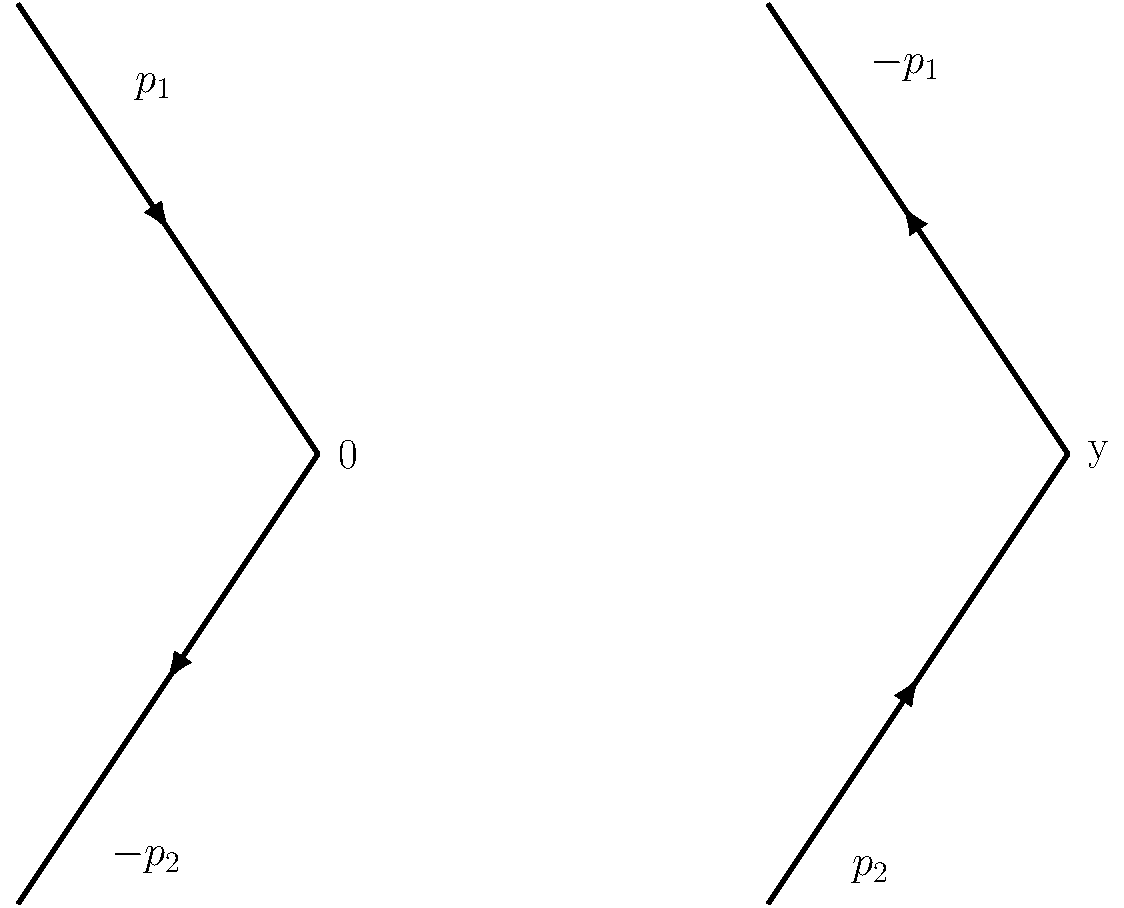
\includegraphics[scale=0.3]{Figures/DrellYanWilsonLoop.pdf}
    \caption{Integration contour for the eikonal approximation in the Drell-Yan process, and $y=(y^{0},\Vec{0})$.}
    \label{fig:DYWilsonLoop}
\end{figure}
%%%%%%%%%%%%%%%%%%%%%%%%%%%%%%%%%%

We can now do the same as we did in \cref{sec:threshold factorization} and use factorization properties of cross sections to define eikonal distributions responsible for the collinear divergences in $\sigma_{ij}^{(\text{eik})}$. 
So the next object to consider is the eikonal analogue to the light-cone distributions $f_{i/i}$. In the limit $x\rightarrow 1$, parton-in-parton distributions can be shown to take the form \cite{Korchemsky:1988si}\footnote{Again, there is an implicit average and sum over colour in the expectation value.}
\begin{align}
    f_{i/i}^{(\text{eik})}(x,\mu,\epsilon)&=\frac{Q}{2}\int_{-\infty}^{\infty}\frac{dy^{-}}{2\pi}\,e^{iy^{-}(1-x)Q/2}\bra{0}\Bar{\mathcal{T}}\{\mathcal{U}_{-p_1}[y,\infty]\}\mathcal{T}\{\mathcal{U}_{p_1}[0,\infty]\}\ket{0}\nonumber
    \\
    &=\frac{Q}{2}\int_{-\infty}^{\infty}\frac{dy^{-}}{2\pi}\,e^{iy^{-}(1-x)Q/2}\mathcal{W}_{\gamma_{p_1}}(y)\,,
\end{align}
where the path $\gamma_{p_1}$ is the $p_1$ part of $\gamma_{DY}$. 

By using these eikonal distributions the eikonal cross section can be written as
\begin{align}\label{eq:1st eikonal cross section}
    \sigma_{ij}^{(\text{eik})}(w,Q,\mu,\alpha_s,\epsilon)&=\int dw_1 dw_2 dw'\,f_{i/i}^{(\text{eik})}(w_1,\mu,\epsilon)\,f_{i/i}^{(\text{eik})}(w_2,\mu,\epsilon)\,\omega_{ij}^{(\text{eik})}(w',Q,\mu,\alpha_s)\nonumber
    \\
    &\hspace{1cm}\delta(w-w_1-w_2-w')\,.
\end{align}
where we defined the energy fractions $w=1-\tau$, $w_1=1-x_1$, $w_2=1-x_2$ and $w'=1-z$. 

In \cref{sec:threshold factorization} we were working in Mellin space, so by taking the Mellin transform of \cref{eq:1st eikonal cross section} we obtain 
\begin{align}\label{eq:eikonal approcximation of partonic}
    \Me{\sigma}^{(\text{eik})}(N,Q,\mu,\alpha_s,\epsilon)=\Me{f}_{i/i}^{(\text{eik})}(N,\mu,\epsilon)\,\Me{f}_{j/j}^{(\text{eik})}(N,\mu,\epsilon)\,\Me{\omega}_{ij}^{(\text{eik})}(N,Q,\mu,\alpha_s)\,,
\end{align}
where we have used that the Mellin transform of the delta function is
\begin{align}
    \int_{0}^{1}d\tau\tau^{N-1}\,\delta(1-\tau-(1-x_1)-(1-x_2)-(1-z))=e^{-N(1-x_1+1-x_2+1-z)}\,,
\end{align}
where $e^{-N(1-x)}=x^{N-1}$ in the large $N$ limit. The result in \cref{eq:eikonal approcximation of partonic} is the eikonal approximation of \cref{eq:partonic analogue to hadronic in mellin }. 

We can also make an eikonal approximation of the near threshold cross section \cref{eq:threshold factorization Mellin}, which can be constructed in a similar fashion as we have done for \cref{eq:eikonal approcximation of partonic}, given by
\begin{align}\label{eq:eikonal approcximation of near threshold}
    \Me{\sigma}^{(\text{eik})}(N,Q,\mu,\alpha_s,\epsilon)=\Me{J}_{i/i}^{(\text{eik})}(N,\mu,\epsilon)\,\Me{J}_{j/j}^{(\text{eik})}(N,\mu,\epsilon)\,\Me{S}_{ij}(N,Q,\mu,\alpha_s)\,,
\end{align}
where we have used that the soft function by definition contains the soft contributions, i.e. $S_{ij}=S_{ij}^{(\text{eik})}$. Then we can use that \cref{eq:eikonal approcximation of partonic} and \cref{eq:eikonal approcximation of near threshold} must be equal near threshold, giving
\begin{align}\label{eq:partonic eikonal with soft function}
    \Me{\omega}_{ij}^{(\text{eik})}(N,Q,\mu,\alpha_s)=\frac{\Me{J}_{i/i}^{(\text{eik})}(N,\mu,\epsilon)\,\Me{J}_{j/j}^{(\text{eik})}(N,\mu,\epsilon)}{\Me{f}_{i/i}^{(\text{eik})}(N,\mu,\epsilon)\,\Me{f}_{j/j}^{(\text{eik})}(N,\mu,\epsilon)}\Me{S}_{ij}(N,Q,\mu,\alpha_s)\,.
\end{align}

Apart from contributions from hard virtual gluons, \cref{eq:partonic eikonal with soft function} is the eikonal approximation of \cref{eq:partonic hard function ratio in mellin}. This means that we have an expression for the soft function $\Me{S}$, so if we solve for the soft function in \cref{eq:partonic eikonal with soft function} and insert it into \cref{eq:partonic hard function ratio in mellin}, we find that the hard partonic function can be written as
\begin{align}\label{eq:partonic and eikonal plus ration}
    \Me{\omega}_{ij}(N,Q,\mu,\alpha_s(\mu))=&\Big[\frac{\Me{J}_{i/i}(N,Q,\epsilon)\Me{J}_{j/j}(N,Q,\epsilon)}{\tilde{f}_{i/i}(N,\mu,\epsilon)\tilde{f}_{j/j}(N,\mu,\epsilon)}\Big]\Big[\frac{\Me{f}_{i/i}^{(\text{eik})}(N,\mu,\epsilon)\,\Me{f}_{j/j}^{(\text{eik})}(N,\mu,\epsilon)}{\Me{J}_{i/i}^{(\text{eik})}(N,\mu,\epsilon)\,\Me{J}_{j/j}^{(\text{eik})}(N,Q,\epsilon)}\Big]\nonumber
    \\
    &H_{ij}(Q,\alpha_{s}(\mu))\,\Me{\omega}_{ij}^{(\text{eik})}(N,Q,\mu,\alpha_s)\,,
\end{align}
where both of these ratios are defined such that they cancel each others collinear divergences. This expression looks daunting, but as previously mentioned the ratios can be simplified by using the renormalization group properties of the distributions, which we will do in \cref{sec:RGE for parton in parton}. The eikonal function $\omega_{ij}^{(\text{eik})}$ is the main function of interest, as it contains the parts where soft contributions cancel to give the large logarithms.

We have managed to bring the hard partonic function $\Me{w}_{ij}$ on a fully factorized form in terms of the eikonal function $\Me{\omega}_{ij}^{(\text{eik})}$. It might not have been obvious what the point of this whole refactorization is, but the idea is that we now have an expression where the IR-divergences are grouped into different terms responsible for different regions of phase space. Before we go into details of how to find the eikonal function $\Me{w}_{ij}
^{\text{(eik)}}$ we will take a closer look at the renormalization properties of Wilson lines and the renormalization group equations for the distributions in \cref{eq:partonic and eikonal plus ration}. The reason for taking this slight detour is to introduce the cusp anomalous dimension, which we will have use for later. %The procedure to calculate it is very complicated, but we will later try to explain how it can be done.

%But first we will in the next couple of sections look at renormalization properties of parton-in-parton distributions in the $x\rightarrow 1$ limit and the renormalization properties of Wilson lines.

\subsection*{Overview of IR-divergences}
We have tried to point out as we went along where the divergences in the different expressions above are, but let us try to make that more clear.

First of all, the hadronic cross section $\sigma_{h_{1}h_{2}}$ is of course finite. On the other hand, we observed in a fixed order calculation at NLO that the partonic function $\omega_{ij}$ has collinear divergences. To single this contribution out we defined a partonic analog to the hadronic cross section \cref{eq:partonic analogue to hadronic in mellin } in Mellin space, in such a way that the parton-in-parton distributions $f_{i/i}$ were responsible for these collinear divergences, rendering $\omega_{ij}$ IR-finite. The consequence of this definition is that the parton-in-hadron distributions $f_{i/h}$ do not contain any singularities, which is important as one wants to take these from experimental measurements. 

From there we went on to write down a near threshold form of the partonic cross section \cref{eq:threshold factorization Mellin}, where all collinear singularities are included in the jet subprocesses $J_{i/i}$. The hard subprocess $H$ includes only lines that are off-shell and does not contain any large logarithms. The soft subprocess $S_{ij}$ is defined to include all wide angle soft radiation.

Finally we made an eikonal cross section $\sigma_{ij}^{(\text{eik})}$ in \cref{eq:eikonal cross section wilson loop}, which contains collinear singularities due to the light-like momenta $p_1$ and $p_2$ of the incoming partons\footnote{Or rather due to the light-like directional vectors $n_{1}$ and $n_{2}$ along the momenta $p_1$ and $p_2$.}. We factorized this cross section in \cref{eq:eikonal approcximation of partonic} and \cref{eq:eikonal approcximation of near threshold} such that $f_{i/i}^{(\text{eik})}$ and $J_{i/i}^{(\text{eik})}$ are responsible for these collinear divergences. The eikonal cross section $\sigma_{ij}
^{(\text{eik})}$ also contains soft divergences, but according to the KLN-theorem these cancel in the sum over all final states, leading to large logarithms. Hence, the soft function $S_{ij}$ and the eikonal function $\omega_{ij}
^{(eik)}$ are free of IR-divergences. 
% \section{Renormalization of Wilson Lines}
In this section we will look at the renormalization properties of Wilson lines, and in particular find the cusp anomalous dimension. Later we will see that the cusp anomalous dimension appear in evolution equations for parton distributions and in the exponent of the exponentiated eikonal cross section. Hence, it is a fundamental ingredient in resummation with Wilson lines. 

There are two kinds of cusp anomalous dimensions, one is for Wilson lines on light-cone and one for Wilson lines off light-cone. We are considering the case of massless quarks, so the Wilson lines on light-cone is those of main focus, i.e. we need the on light-cone cusp anomalous dimension. We will show one way of calculating it in the next section, but first we will show how it appears.


In order to find the behaviour of Wilson lines at different scales, we can use the basic principle that the bare definition must be independent on the renormalization scale, i.e. the bare Wilson line satifies
\begin{align}\label{eq:bare wilson line}
    \mu\dv{}{\mu}\mathcal{U}_{\gamma}^{0}=0\,.
\end{align}
The bare Wilson line is given in terms of the bare coupling $g_0$ and the bare gauge field. Let us then rescale the field as in \cref{eq:rescaled gauge field QCD}, and use \cref{eq:counterterms} to define the relation
\begin{align}
    \mathcal{Z}_{3}^{1/2}g_{0}=\mathcal{Z}_{g}g\,,
\end{align}
giving the renormalized Wilson line\footnote{The scale factor $\mu$ is as usual hidden in g, i.e. we always make the substitution $g(\mu)\rightarrow\mu^{d-4}g$.}
\begin{align}
    \mathcal{U}_{\gamma}(g,\mu)=\mathcal{P}\exp{ig\mathcal{Z}_{g}\int_{\gamma}dz^{\mu}A_{\mu}(z)}\,.
\end{align}
A smooth Wilson with no cusps is completely renormalized as long as the coupling and the field is renormalized \cite{POLYAKOV1980171,DOTSENKO1980527}. Hence, by applying \cref{eq:bare wilson line} we would find a regular Callan-Symanzik equation. 

However, since we are studying a quark--antiquark pair that meets at a point and annihilates we are in interested in paths with cusps. These cusps will contribute with additional UV-divergences, so-called cusp divergences. A cusp in a Wilson line is characterized by two directional vectors $n_{1}^{\mu}$ and $n_{2}^{\mu}$ and the cusp divergence is a function of the angle $\chi$ between these two vectors. In Minkowski space this angle is defined as
\begin{align}\label{eq:Minkowski space angle}
    \cosh \chi=\frac{n_{1}\cdot n_2}{\sqrt{n_{1}^{2}n_{2}^{2}}}\,,
\end{align}
and the Wilson line will acquire a dependency on the regulator $\epsilon$ in dimensional regularization, i.e. $\mathcal{U}_{\gamma}(g,\mu,\epsilon)$. If both vectors are off light-cone, i.e. $n_{1}^{2}\neq 0$ and $n_{2}^{2}\neq 0$, the cusp divergences can be treated multiplicatively by introducing a multiplicative factor $\mathcal{Z}_{\text{cusp}}$ \cite{DOTSENKO1980527,Korchemsky:1987wg}
\begin{align}
    \widetilde{\mathcal{U}}_{\gamma}(g,\mu)=\mathcal{Z}_{\text{cusp}}(\chi,g,\mu,\epsilon)\,\mathcal{U}_{\gamma}(g,\mu,\epsilon)
\end{align}
giving the Callan-Symanzik equation
\begin{align}
    \Big(\mu\pdv{}{\mu}+\beta(g)\pdv{}{g}\Big)\,\ln\widetilde{\mathcal{U}}_{\gamma}(g,\mu)=\Gamma_{\text{cusp}}(\chi,g)\,,
\end{align}
where the cusp anomalous dimension is given by
\begin{align}
    \Gamma_{\text{cusp}}(\chi,g)=\lim_{\epsilon\to 0}\frac{\mu}{\mathcal{Z}_{\text{cusp}}}\dv{}{\mu}\mathcal{Z}_{\text{cusp}}(\chi,g,\epsilon)=\lim_{\epsilon\to 0}\dv{}{\ln\mu}\ln\mathcal{Z}_{\text{cusp}}(\chi,g,\epsilon)\,.
\end{align}
In regular UV-renormalization we have that the renormalization factor removes the $\epsilon$ dependence via counterterms, see \cref{sec:Renormalization}. Hence, we can calculate a Wilson line with cusps in perturbation theory and use $\mathcal{Z}_{\text{cusp}}$ to pull out the divergent part.  

If one or both vectors are on the light-cone, we can no longer use the multiplicative renormalization technique. This follows from the fact that for light-like vectors, \cref{eq:Minkowski space angle} blows up, and creates additional divergences. In dimensional regularization these additional divergences are double poles, i.e. of the form $1/\epsilon^{2}$. In \cref{sec:NLO drell yan calculation} we found that by adding the real and virtual gluon emission the double pole vanished and the cross section acquired large logarithmic dependancy. Thus, treating the $1/\epsilon
^{2}$ divergence would give a way of managing these large contributions by the renormalization properties of Wilson lines. 

Now, there is a relation between the on light-cone and off light-cone cusp anomalous dimension that we can use. In \cite{KORCHEMSKAYA1992169} it was found that the relation between the two in the limit of large $\chi$, is given by
\begin{align}\label{eq:off lightcone and on lightcone}
    \lim_{\chi\rightarrow\infty}\Gamma_{\text{cusp}}(\chi,g)=\chi\Gamma_{\text{cusp}}(g)+\mathcal{O}(\chi^{0})\,.
\end{align}
In this large limit, it follows from \cref{eq:Minkowski space angle} that
\begin{align}\label{eq:large minkowski limit}
    \chi=\ln\Big(\frac{2n_{1}\cdot n_{2}}{\sqrt{n_{1}^{2}n_{2}^{2}}}\Big)\,.
\end{align}
We observe that if we differentiate \cref{eq:off lightcone and on lightcone} with respect to $\ln n_{1}\cdot n_2$ we remove the troublesome denominator that blows up for light-like vectors. Therefore, we can write the on light-cone cusp anomalous dimension as\footnote{If the $\epsilon\rightarrow 0$ limit seem sketchy it is ment to be happen after the differentiation has been performed.}
\begin{align}\label{eq:on lightcone cusp anomalous}
    \Gamma_{\text{cusp}}(g)=\lim_{\epsilon\to 0}\dv{}{\ln n_1\cdot n_2}\dv{}{\ln\mu}\ln\mathcal{Z}_{\text{cusp}}(\chi,g,\epsilon)\,,
\end{align}
which is the expression we will use after we have calculated $\Gamma(\chi,g)$ in the next section.
%We can then integrate over $n_{1}\cdot n_2$, giving the modified Callan-Symanzik equation
%\begin{align}
%    \Big(\mu\pdv{}{\mu}+\beta(g)\pdv{}{g}\Big)\,\ln\widetilde{\mathcal{U}}_{\gamma}(g,\mu)=\Gamma_{\text{cusp}}(g)\ln n_{1}\cdot n_{2}+\Gamma(g)\,,
%\end{align}
%where $\Gamma(g)$ is some integration constant.

Wilson lines with endpoints will also have their own renormalization factors, and a corresponding endpoint anomalous dimension \cite{KORCHEMSKY1986459}. But we will only consider semi-infinite Wilson lines with endpoint at infinity. These contains IR-divergnces, which we will treat with an exponential regulator that suppress such contributions. 

\subsection{One-Loop Cusp Anomalous Dimension}
To calculate the one-loop cusp anomalous dimension, we consider the case of two semi-infinite Wilson lines bounded from below, see \cref{eq:semi-infinite Wilson line 0-to-infty}. We denote these as
\begin{align}
    \mathcal{U}_{\gamma_1}[\infty,0]&=\mathcal{P}\exp\Big(ig\int_{0}^{\infty}d\lambda_1\,n_{1}\cdot A(\lambda_1 n_1)\Big)\,,
    \\
    \mathcal{U}_{\gamma_2}[\infty,0]&=\mathcal{P}\exp\Big(ig\int_{0}^{\infty}d\lambda_2\,n_{2}\cdot A(\lambda_2 n_2)\Big)\,.
\end{align}

To construct the geometry of the diagrams in \cref{fig:one loop cusp anomalous dimension}, we use that Wilson lines are path-transitive and can be written as the composition\footnote{We could have used $\mathcal{W}_{DY}$ to calculate the cusp anomalous dimension, but that calculation is more complicated.}
\begin{align}\label{eq:wedged wilson line}
    \mathcal{U}_{\wedge}(0)=\mathcal{U}_{\gamma_1}[\infty,0]\mathcal{U}_{\gamma_2}[\infty,0]\,.
\end{align}
Expanding \cref{eq:wedged wilson line} to $\mathcal{O}(g^{2})$, we find
\begin{align}\label{eq:two wilson expansion}
    \mathcal{U}_{\wedge}(0)&=1+igt^{a}n_{1}^{\mu}\int_{0}^{\infty}d\lambda_1\,A_{\mu}^{a}(\lambda_{1}n_1)+igt^{b}n_{2}^{\mu}\int_{0}^{\infty}d\lambda_2\,A_{\mu}^{b}(\lambda_{2}n_2)\nonumber
    \\
    &\hspace{1cm}-g^{2}t^{a}t^{b}n_{1}^{\mu}n_{2}^{\nu}\int_{0}^{\infty}d\lambda_1\int_{0}^{\infty}d\lambda_2\,A_{\mu}^{a}(\lambda_1n_1)A_{\nu}^{b}(\lambda_2n_2)\,,
\end{align}
which follows from the expansions we discussed in \cref{sec:wilson line properties}. But in \cref{sec:wilson line properties} we integrated over $\lambda$ directly by Fourier transforming the fields, giving \cref{eq:semi-infinite Wilson line 0-to-infty}. In momentum space, we have IR-divergences when $n\cdot k\rightarrow 0$ and $k^{2}\rightarrow 0$. These originate from the Wilson line propagator and after the gauge fields have been Wick contracted to give the gauge field propagator. However, it is easier to work in coordinate space for this calculation. The IR-divergence in coordinate space originates from $\lambda\rightarrow\infty$, so to treat it we insert an exponential regulator in the exponent of the Wilson lines
\begin{fmffile}{wilsonone}
\begin{figure}
\centering
\begin{fmfgraph*}(150,100)
\fmfleft{i1} 
\fmfright{o1,o2}
\fmf{fermion}{i1,v1}
\fmf{fermion}{i1,v2}
\fmf{plain}{v1,o1}
\fmf{plain}{v2,o2}
\fmflabel{$\lambda_1 n_1$}{v2}
\fmflabel{$\lambda_2 n_2$}{v1}
\fmffreeze
\fmf{gluon}{v1,v2}
\end{fmfgraph*}
\hspace{1cm}
\begin{fmfgraph*}(150,100)
\fmfleft{i1} 
\fmfright{o1,o2}
\fmf{fermion}{i1,o1}
\fmf{plain,label=$\lambda_{1}n$,l.side=left}{i1,v2}
\fmf{fermion}{v2,v3}
\fmf{plain, label=$\lambda_2 n$,l.side=left}{v3,o2}
\fmffreeze
\fmf{gluon,left,tension=0}{v2,v3}
\end{fmfgraph*}
\caption{Wilson line diagrams contributing to the one-loop cusp anomalous dimension $\Gamma(\chi,g)$.}
\label{fig:one loop cusp anomalous dimension}
\end{figure}
\end{fmffile}
%%%%%%%%%%%%%%
\begin{align}\label{eq:IR regularized Wilson line}
    \mathcal{U}^{\delta}[\infty,0]=\mathcal{P}\exp(ig\int_{0}^{\infty}d\lambda\,n\cdot A(\lambda n)e^{-\delta\lambda\sqrt{-n^{2}}})\,,
\end{align}
which was proposed for Wilson line calculations in \cite{article}. The idea here is that $\delta\sqrt{-n^{2}}>0$, so that the exponential factor smoothly cuts off the $\lambda\rightarrow\infty$ contribution. This is guaranteed to yield an IR-finite result for the integral in \cref{eq:IR regularized Wilson line}, and all the remaining poles are of UV origin, i.e. $\lambda\rightarrow 0$.  

\subsubsection*{One-Loop Calculation}
To calculate the full cusp anomalous dimension $\Gamma_{\text{cusp}}(\chi,g)$, we would have to calculate both diagrams in \cref{fig:one loop cusp anomalous dimension}. But as we can see, the diagram on the right-hand does not depend on the cusp angle as the radiation is from the same line, so to find $\Gamma_{\text{cusp}}(g)$ we only focus on the left-hand diagram. 

To calculate this contribution we consider the expectation value
\begin{align}\label{eq:wedge wilson loop}
    \mathcal{W}_{\wedge}=\bra{0}\mathcal{T}\mathcal{U}_{\wedge}(0)\ket{0}\,
\end{align}
where the $\mathcal{T}$ is the time-ordering operator. Expanding \cref{eq:wedge wilson loop} to $\mathcal{O}(g^{2})$ using the expansion in \cref{eq:two wilson expansion}, will give
\begin{align}
    \mathcal{W}_{\wedge}&=1+\mathcal{W}_{\wedge}^{(1)}\nonumber
    \\
    &=1-g^{2}t^{a}t^{b}n_{1}^{\mu} n_{2}^{\mu}\int_{0}^{\infty}d\lambda_{1}\int_{0}^{\infty}d\lambda_{2}\,D_{\mu\nu}^{ab}(\lambda_{1}n_1-\lambda_{2}n_2)\,,
\end{align}
where we Wick contracted the emitted gluons to give the propagator. The propagator in coordinate space is given by \cite{article},
\begin{align}
    D_{\mu\nu}^{ab}(x-y)=-\mathcal{N}\frac{g_{\mu\nu}\delta^{ab}}{(-(x-y)^{2}+i\epsilon)^{d/2-1}}\,,
\end{align}
where
\begin{align}
    \mathcal{N}=\frac{\Gamma(d/2-1)}{4\pi^{d/2}}\,.
\end{align}
Here we should keep in mind that the Feynman prescription $i\epsilon$ and the regulator $\epsilon$ are not the same when we expand in $d=4-2\epsilon$. 

Let us then insert the IR-regulator given in \cref{eq:IR regularized Wilson line}, giving the expression
\begin{align}\label{eq:amplitude radiation wilson line cusp}
    \mathcal{W}_{\wedge}^{(1)}&=-g^{2}t^{a}t^{b}n_{1}^{\mu} n_{2}^{\mu}\int_{0}^{\infty}d\lambda_{1}\int_{0}^{\infty}d\lambda_{2}\,D_{\mu\nu}^{ab}(\lambda_{1}n_1-\lambda_{2}n_2)\,e^{-\delta(\lambda_1\sqrt{-n_{1}^{2}}+\lambda_2\sqrt{-n_{2}^{2}})}\nonumber
    \\
    &=g^{2}C_{F}\mathcal{N}(\epsilon)n_{1}\cdot n_{2}\int_{0}^{\infty}d\lambda_{1}\int_{0}^{\infty}d\lambda_{2}\,\frac{e^{-\delta(\lambda_1\sqrt{-n_{1}^{2}}+\lambda_2\sqrt{-n_{}^{2}})}}{(-(\lambda_{1}n_{1}-\lambda_{2}n_{2})^{2})^{1-\epsilon}}\,.
\end{align}
To evaluate the integrals we can make the change of variables
\begin{align}
    \lambda_1&=\frac{\alpha x}{\sqrt{-n_{1}^{2}}}\,,
    \\
    \lambda_{2}&=\frac{\alpha(1-x)}{\sqrt{-n_{2}^{2}}}\,,
\end{align}
where $x\in[0,1]$ and $\alpha\in[0,\infty)$, giving the Jacobian
\begin{align}
    \mathcal{J}=\frac{\alpha}{\sqrt{n_{1}^{2}n_{2}^{2}}}\,.
\end{align}
With these changes we get the following integral
\begin{align}
    I&=\int_{0}^{\infty}d\lambda_{1}\int_{0}^{\infty}d\lambda_{2}\,\frac{e^{-\delta(\lambda_1\sqrt{-n_{1}^{2}}+\lambda_2\sqrt{-n_{}^{2}})}}{(-(\lambda_{1}n_{1}-\lambda_{2}n_{2})^{2})^{1-\epsilon}}\nonumber
    \\
    &=\frac{1}{\sqrt{n_{1}^{2}n_{2}^{2}}}\int_{0}^{1}dx \frac{1}{(x^{2}+(1-x)^{2}+2x(1-x)\cosh\gamma)^{1-\epsilon}}\int_{0}^{\infty}d\alpha\,e^{-\delta\alpha}\alpha^{-1+2\epsilon}\,,
\end{align}
where we defined 
\begin{align}\label{eq:gamma minkowski}
    \cosh\gamma=-\frac{n_{1}\cdot n_{2}}{\sqrt{n_{1}^{2}n_{2}^{2}}}\,,
\end{align}
and by inserting this back into \cref{eq:amplitude radiation wilson line cusp}, we get
\begin{align}
    \mathcal{W}_{\wedge}^{(1)}=-g^{2}C_{F}\mathcal{N}(\epsilon)\int_{0}^{1}dx\frac{\cosh\gamma}{(x^{2}+(1-x)^{2}+2x(1-x)\cosh\gamma)^{1-\epsilon}}\int_{0}^{\infty}d\alpha\,e^{-\delta\alpha}\alpha^{-1+2\epsilon}\,.
\end{align}

Let us evaluate the $\alpha$ integral by another change of variable $y=\alpha\delta$, giving
\begin{align}
    \int_{0}^{\infty}d\alpha\,e^{-\delta\alpha}\alpha^{-1+2\epsilon}=\delta^{-2\epsilon}\int_{0}^{\infty}dy\,e^{-y}y^{-1+2\epsilon}=\delta^{-2\epsilon}\,\Gamma(2\epsilon)\,,
\end{align}
where we used the integral representation of the Gamma function. This gamma function has the expansion as $\epsilon\rightarrow 0$
\begin{align}
    \Gamma(2\epsilon)=\frac{1}{2\epsilon}+\mathcal{O}(\epsilon^{0})\,.
\end{align}

The $x$ integral can be rewritten in terms of the hypergeometric function $_{2}F_{1}$. However, we want the expansion in the limit $\epsilon\rightarrow 0$, so it is inconvenient to use this representation. Let us instead set $\epsilon=0$ in this integral, giving
\begin{align}
    \int_{0}^{1}dx\frac{\cosh\gamma}{(x^{2}+(1-x)^{2}+2x(1-x)\cosh\gamma)}=\gamma\coth\gamma\,.
\end{align}
This integral would not be convergent without the definition of $\gamma$ in \cref{eq:gamma minkowski}. But we want our result in terms of $\chi$, and from \cref{eq:Minkowski space angle} these are related in the following way
\begin{align}
    \cosh\gamma&=-\cosh\chi=\cosh(\chi+i\pi)\,,
\end{align}
giving
\begin{align}
    \gamma=\chi+i\pi
\end{align}
and
\begin{align}
    \coth(\chi+i\pi)=\coth\chi\,.
\end{align}
Also, we can safely neglect the terms that are non singular for $\epsilon\rightarrow 0$, i.e. $\delta^{-2\epsilon}\rightarrow 1$ and $\mathcal{N}(\epsilon)\rightarrow 1/4\pi^{2}$. This removes the IR regulator $\delta$ from the expression in a smooth way. Using all these relations, we find that the $\mathcal{O}(g^{2})$ expansion of the Wilson loop expectation value takes the form
\begin{align}\label{eq:one loop wedge wilson loop}
    \mathcal{W}_{\wedge}^{(1)}&=-g^{2}\,C_{F}\,\mathcal{N}(\epsilon)\,\delta^{-2\epsilon}\,\Gamma(2\epsilon)\,\gamma\coth\gamma\nonumber
    \\
    &=-g^{2}\,C_{F}\,\frac{1}{4\pi^{2}}\,\frac{1}{2\epsilon}\,(\chi+i\pi)\coth\chi\,.
\end{align}
As mentioned above, this is only one contribution to the cusp anomalous dimension $\Gamma_{cusp}(\chi,g)$. But the other contribution does not depend on the cusp angle, so when we perform the differentiation with respect to $\ln n_1\cdot n_2$ it will not contribute to $\Gamma_{cusp}(g)$ that we are interested in.

\subsubsection*{Cusp Anomalous Dimension $\Gamma_{\text{cusp}}(g)$}
In \cref{eq:on lightcone cusp anomalous} we had that the cusp anomalous dimension for Wilson lines on light-cone could be written as
\begin{align}
    \Gamma_{\text{cusp}}(g)=\lim_{\epsilon\to 0}\dv{}{\ln n_1\cdot n_2}\dv{}{\ln\mu}\ln\mathcal{Z}_{\text{cusp}}(\chi,g,\epsilon)\,.
\end{align}
To find $\Gamma_{\text{cusp}}(g)$ we can now use that $\mathcal{Z}_{\text{cusp}}$ is used to cancel the $\epsilon$ divergence from the Wilson line in \cref{eq:one loop wedge wilson loop}. We can also introduce the dependence on the scale $\mu$ in the usual way $g^{2}\rightarrow \mu^{2\epsilon}g^{2}$, giving the cusp factor 
\begin{align}
    \mathcal{Z}_{\text{cusp}}=1+g^{2}\mu^{2\epsilon}C_{F}\frac{1}{4\pi^{2}}\frac{1}{2\epsilon}(\chi+i\pi)\coth\chi\,.
\end{align}
Performing the differentiation and keeping only terms to $\mathcal{O}(g^{2})$, we find
\begin{align}
    \Gamma_{\text{cusp}}(g)&=\lim_{\epsilon\to 0}\dv{}{\ln n_1\cdot n_2}\mu\dv{}{\mu}\ln\Big(1+g^{2}\mu^{2\epsilon}C_{F}\frac{1}{4\pi^{2}}\frac{1}{2\epsilon}(\chi+i\pi)\coth\chi\Big)\nonumber
    \\
    &=\dv{}{\ln n_1\cdot n_2}\Big(g^{2}C_{F}\frac{1}{4\pi^{2}}(\chi+i\pi)\coth\chi\Big)\nonumber
    \\
    &=\frac{g^{2}}{4\pi^{2}}C_{F}\,,
\end{align}
where we in the last differentiation used that $\chi$ is given by \cref{eq:large minkowski limit} in the large limit, and that $\coth\chi=1$ in this limit. At first sight the this might seem a little fishy as the derivative of the logarithm gives the argument in the denominator. But if we expand this denominator it will give a $\mathcal{O}(g^{4})$ term and we are only considering the $\mathcal{O}(g^{2})$ correction. As usual we use that $\alpha_s=g^{2}/4\pi$, giving
\begin{align}\label{eq:one-loop cusp anomalous dimension}
    \Gamma_{\text{cusp}}(\alpha_s)=\frac{\alpha_s}{\pi}C_{F}\,,
\end{align}
which is the well known one-loop cusp anomalous dimension for a Wilson line in the fundamental representation \cite{Korchemsky:1987wg}.  


\section{Exponentiation of Parton-In-Parton Distributions}\label{sec:RGE for parton in parton}
In \cref{sec:QCD and Collinear factorization}, we discussed the renormalization group equation for the parton distribution functions $f_{i/P}(x,\mu)$, i.e. the DGLAP equation. Now we would like to discuss the renormalization group equations for the parton-in-parton disttribution functions $f_{i/i}$. In \cref{sec:lightcone parton in parton distributions} we derived the parton-in-parton distributions, given by
\begin{align}
    f_{i/i}(x)=\int\frac{dy^{-}}{4\pi}e^{-ixp^{+}y^{-}}\bra{q}\overline{\Psi}(y^{-})\gamma^{+}\Psi(0)\ket{q}\,,
\end{align}
where the product in the matrix element are eikonal fermions\footnote{Or particles dressed with Wilson lines.}. In \cite{Korchemsky:1988si} it was found that in the limit $x\rightarrow 1$, the parton-in-parton distributions obeys the evolution equation
\begin{align}\label{eq:RGE partoninparton}
    \mu\dv{}{\mu}f_{i/i}(x,\mu)=\int_{x}^{1}\frac{dz}{z}P_{i/i}\big(\frac{x}{z},\alpha_s\big)f_{i/i}(z,\mu)+\mathcal{O}((1-x)^{0})\,,
\end{align}
where the splitting functions has the asymptotic behaviour 
\begin{align}\label{eq:asymptotic splitting function}
    P_{i/i}(z,\alpha_s)=2\Gamma_{\text{cusp}}^{(i)}(\alpha_s)\Big[\frac{1}{1-z}\Big]_{+}+2C^{(i)}(\alpha_s)\delta(1-z)+\mathcal{O}((1-z)^{0})\,,
\end{align}
which is true to all order \cite{Korchemsky:1988si}, and the one-loop $\Gamma_{\text{cusp}}^{(q,\bar{q})}$ is the one we found in \cref{eq:one-loop cusp anomalous dimension}. We can verify this behaviour by taking the limit $z\rightarrow 1$ of the splitting functions we found in \cref{eq:qq splitting function} and \cref{eq:gg splitting function}, giving
\begin{align}
    P_{q/q}(z)&=2C_{F}\frac{\alpha_s}{\pi}\Big(\Big[\frac{1}{1-z}\Big]_{+}+\frac{3}{4}\delta(1-z)\Big)+\mathcal{O}(\alpha_{s}^{2})\,,
    \\
    P_{g/g}(z)&=2\frac{\alpha_s}{\pi}\Big(C_{A}\Big[\frac{1}{1-z}\Big]_{+}+\frac{\beta_{0}}{4}\delta(1-z)\Big)+\mathcal{O}(\alpha_{s}^{2})\,,
\end{align}
where $\beta_0$ is the one-loop beta coefficient, see \cref{eq:beta one-loop}, and we observe that the cusp anomalous dimension for $q,\bar{q}$ corresponds to the one we found in \cref{eq:one-loop cusp anomalous dimension}. We also observe that the cusp anomalous dimension for $i=g$ is given by
\begin{align}
    \Gamma_{\text{cusp}}^{(g)}(\alpha_s)=\frac{\alpha_s}{\pi}C_{A}+\mathcal{O}(\alpha_{s}^{2})\,,
\end{align}
which is just a matter of making the calculation we did in \cref{eq:one-loop cusp anomalous dimension} by using Wilson lines in the adjoint representation giving the Casimir invariant $C_{A}$. We can also read of the one-loop expression for $C^{(i)}$, given by
\begin{align}
    C^{(q,\bar{q})}(\alpha_s)&=\frac{\alpha_s}{\pi}\frac{3}{4}C_{F}+\mathcal{O}(\alpha_{s}^{2})\,,\label{eq:C for quarks}
    \\
    C^{(g)}(\alpha_s)&=\frac{\alpha_s}{\pi}\frac{\beta_{0}}{4}+\mathcal{O}(\alpha_{s}^{2})\,,\label{eq:C for gluons}
\end{align}

In order to solve \cref{eq:RGE partoninparton} we take the Mellin transform, giving the large $N$ equation\footnote{Remember that $z\rightarrow 1$ corresponds to to large N.}
\begin{align}
    \mu\dv{}{\mu}f_{i/i}(N,\mu)=P_{i/i}(N,\alpha_{s})f_{i/i}(N,\mu)+\mathcal{O}(1/N)\,.
\end{align}
where the moments of the splitting function takes the form
\begin{align}
    P_{i/i}(N,\alpha_s)&=2\Gamma_{\text{cusp}}^{(i)}(\alpha_s)\int_{0}^{1}dz\,z^{N-1}\Big[\frac{1}{(1-z)_{+}}\Big]+2C^{(i)}(\alpha_s)\int_{0}^{1}dz\,z^{N-1}\delta(1-z)\nonumber
    \\
    &=-2\Gamma_{\text{cusp}}^{(i)}(\alpha_s)\ln\bar{N}+2C^{(i)}(\alpha_s)\,,
\end{align}
where we neglect constant terms from the Mellin transform, see \cref{eq:App mellin of ln plus dist}. These constant terms would reproduce the constant terms we neglected in \cref{eq:Mellin space NLO of omegaqbarq}, so we do the same here. Hence, the evolution equation in Mellin space take the form
\begin{align}
    \dv{}{\ln\mu}\ln f_{i/i}(N,\mu)=-2\Gamma_{\text{cusp}}^{(i)}\ln\bar{N}+2C^{(i)}(\alpha_s)\,.
\end{align}
with the solution
\begin{align}\label{eq:RGE parton in parton}
    f_{i/i}(N,\mu)=\exp{-\int_{0}^{\mu^{2}}\frac{d\mu'^{2}}{\mu'^{2}}\Big(\Gamma_{\text{cusp}}^{(i)}(\alpha_{s}(\mu'))\ln\bar{N}-C^{(i)}(\alpha_{s}(\mu'))\Big)}\,.
\end{align}
where we have chosen the initial condition $f_{i/i}(N,\mu=0)=1$.

For the eikonal distributions $f_{i/i}^{(\text{eik})}$ there is a slight modification. We want them to be sum of plus distributions, so from \cref{eq:asymptotic splitting function} we must have that $C^{i}=0$. The solution can then be written as
\begin{align}\label{eq:RGE parton in parton eikonal}
    f_{i/i}^{(\text{eik})}=\exp{-\int_{0}^{\mu^{2}}\frac{d\mu'^{2}}{\mu'^{2}}\Gamma_{\text{cusp}}^{(i)}(\alpha_{s}(\mu')\ln\bar{N}}\,.
\end{align}
Notice that the choice of the lower boundary diverges for $\mu\rightarrow 0$, which will be used later to cancel divergences coming from $\Me{\sigma}^{\text{(eik)}}(N,\epsilon)$. The equations for $J_{i/i}$ and $J_{i/i}^{(\text{eik})}$ are completely analogous. 

\subsection{Hard Virtual Gluons}
With the solutions in \cref{eq:RGE parton in parton} and \cref{eq:RGE parton in parton eikonal} we are now ready to compute the ratios of distributions we had in \cref{eq:partonic and eikonal plus ration}. But first, we mentioned in \cref{sec:factorization soft gluons} that the main difference between the partonic function $\omega_{ij}$ and its eikonal approximation $\omega_{ij}^{(\text{eik})}$ are contributions $G_{ij}(Q,\mu)$ from hard virtual gluons \cite{KORCHEMSKY1993433}. So in general, we can write the relation between the two as
\begin{align}\label{eq:relation w and eikonal w}
    \Me{\omega}_{ij}(N,Q,\mu,\alpha_{s}(\mu))=H_{ij}(Q,\alpha_{s}(\mu))\,G_{ij}(Q,\mu)\,\Me{\omega}_{ij}^{(\text{eik})}(N,Q,\mu,\alpha_s)\,,
\end{align}
where $H(Q)$ is the same hard process without large logarithms. If we compare this expression with \cref{eq:partonic and eikonal plus ration}, we find that the hard virtual contributions are entirely describes by the ratios 
\begin{align}\label{eq:hard virtual gluons}
    G_{ij}(Q,\mu)=\Big[\frac{\Me{J}_{i/i}(N,Q,\epsilon)\Me{J}_{j/j}(N,Q,\epsilon)}{\tilde{f}_{i/i}(N,\mu,\epsilon)\tilde{f}_{j/j}(N,\mu,\epsilon)}\Big]\Big[\frac{\Me{f}_{i/i}^{(\text{eik})}(N,\mu,\epsilon)\,\Me{f}_{j/j}^{(\text{eik})}(N,\mu,\epsilon)}{\Me{J}_{i/i}^{(\text{eik})}(N,Q,\epsilon)\,\Me{J}_{j/j}^{(\text{eik})}(N,Q,\epsilon)}\Big]\,,
\end{align}
and as mentioned in \cref{sec:factorization soft gluons}, the two ratios are free of collinear divergences and so is $G(Q,\mu)$.  We can now use the solutions in \cref{eq:RGE parton in parton} and \cref{eq:RGE parton in parton eikonal} to compute the ratios, giving
\begin{align}\label{eq:ratio pdf and eikonal pdf}
    \frac{\Me{f}_{i/i}^{(\text{eik})}(N,\mu,\epsilon)\,\Me{f}_{j/j}^{(\text{eik})}(N,\mu,\epsilon)}{\tilde{f}_{i/i}(N,\mu,\epsilon)\tilde{f}_{j/j}(N,\mu,\epsilon)}=\exp{-2\int_{0}^{\mu^{2}}\frac{d\mu'^{2}}{\mu'^{2}}C^{(i)}(\alpha_{s}(\mu'))}\,,
\end{align}
where the logarithm $\ln\bar{N}$ accompanied by the cusp anomalous dimension has canceled. We have also used that $C^{(i)}=C^{(j)}$ for $i=q$ and $j=\bar{q}$, giving two times $C^{(i)}$\footnote{We choose to use generic subscripts even if we really mean $i=q$. In this way it would be easier to generalize to cases where we also have $i=g$.}. The ratio of jet distributions are equivalent, with the difference of $Q$ instead of $\mu$, i.e.
\begin{align}\label{eq:ratio jets and eikonal jets}
    \frac{\Me{J}_{i/i}(N,Q,\epsilon)\Me{J}_{j/j}(N,Q,\epsilon)}{\Me{J}_{i/i}^{(\text{eik})}(N,Q,\epsilon)\,\Me{J}_{j/j}^{(\text{eik})}(N,Q,\epsilon)}=\exp{2\int_{0}^{Q^{2}}\frac{d\mu'^{2}}{\mu'^{2}}C^{(i)}(\alpha_{s}(\mu'))}\,.
\end{align}
If we insert \cref{eq:ratio pdf and eikonal pdf} and \cref{eq:ratio jets and eikonal jets} into \cref{eq:hard virtual gluons}, we get after reshuffling the ratios that the contribution from hard virtual gluons can be written as
\begin{align}
    G_{ij}(Q,\mu)=\exp{2\int_{\mu^{2}}^{Q^{2}}\frac{d\mu'^{2}}{\mu'^{2}}C^{(i)}(\alpha_{s}(\mu'))}\,,
\end{align}
where we observe that by choosing $Q$ as an argument in the jet distributions, we have a contribution from this expression. But we have already set $Q=\mu$ on several occasions, so for the simplified result we do the same here, giving that $G_{ij}(Q,Q)=1$. With this choice we have from \cref{eq:relation w and eikonal w} that the partonic function $\Me{\omega}_{ij}$ is given by
\begin{align}\label{eq:partonic and eikonal relation}
    \Me{\omega}_{ij}(N,Q,\mu,\alpha_{s}(\mu))=H_{ij}(Q,\alpha_{s}(\mu))\,\Me{\omega}_{ij}^{(\text{eik})}(N,Q,\mu,\alpha_{\mu})\,.
\end{align}

We have reduced the problem of resumming large logarithmic contributions to finding the eikonal function $\Me{\omega}_{ij}^{(\text{eik})}(N)$. Hence, we will in the next section turn our attention back to the eikonal cross section $\Me{\sigma}_{ij}^{\text{eik}}$ and how to calculate it. 

%%%%%%%%% Eikonal cross section %%%%%%%%%%%%%%%%%
\section{The Eikonal Cross Section}
In order to calculate the eikonal cross section $\Me{\sigma}_{ij}^{\text{eik}}$, we look at the Wilson loop expectation value $\mathcal{W}_{DY}$ we found in \cref{sec:factorization soft gluons}. We will first make an $\mathcal{O}(g^{2})$ expansion of the expectation value, and then use the non-Abelian eikonal exponentiation theorem to find the exponentiated form. Then we will use the factorized form of the eikonal cross section in \cref{eq:eikonal approcximation of partonic} to find $\Me{\omega}_{ij}
^{\text{(eik)}}$. 

So let us start from the expectation value
\begin{align}
    \mathcal{W}_{DY}(y)&=\bra{0}\Bar{T}\,\mathcal{U}_{DY}^{\dagger}(y)T\,\mathcal{U}_{DY}(0)\ket{0}\,,
\end{align}
where a one-loop contribution is illustrated in \cref{fig:DYwilsonloopcutpropagator}. By
using the momentum space expansion of Wilson lines derived in \cref{sec:wilson line properties}, we find that to $\mathcal{O}(g^{2})$
\begin{align}\label{eq:order g2 DY wilson loop}
    \mathcal{W}_{DY}=1+g^{2}C_{F}\int\frac{d^{d}k}{(2\pi)^{d}}2\pi\delta^{+}(k^{2})\frac{p_{1}\cdot p_{2}}{p_1\cdot k\,p_2\cdot k}(e^{-iy^{0}k^{0}}-1)\,,
\end{align}
where we have used that $p_{1}^{2}=p_{2}^{2}=0$. We have also used that in diagrams such as \cref{fig:DYwilsonloopcutpropagator}, we have to use a cut gluon propagator \cite{Korchemsky:1992xv}
\begin{align}
    D_{\mu\nu\,+}^{ab}(k)=-\delta^{ab}g_{\mu\nu}2\pi\delta^{+}(k^{2})\,.
\end{align}
To rewrite this further, we can use that the ratio of momenta is invariant under rescaling of $p_1$ and $p_2$. With light-cone coordinates (see \cref{sec:Appendix Light-cone coordinates}), we have that
\begin{align}
    \frac{p_{1}\cdot p_{2}}{p_1\cdot k\,p_2\cdot k}&=\frac{n_{1}\cdot n_{2}}{n_{1}\cdot k\,n_{2}\cdot k}=\frac{1}{k^{+}k^{-}}\label{eq:k+k- relation in calculation}
    \\
    k^{2}&=2k^{+}k^{-}-k_{\perp}^{2}
    \\
    k^{0}&=(k^{+}+k^{-})/\sqrt{2}\label{eq:energy relation lightcone momenta}
\end{align}
where we used that $n_1$ and $n_2$ are light-like vectors. Let us also use the measure $d^{d}k=dk^{+}dk^{-}d^{d-2}k_{\perp}$, such that with the above rewritings the expansion can be rewritten as
\begin{align}\label{eq:W(Drell) to one-loop}
    \mathcal{W}_{DY}&=1+\frac{\alpha_{s}}{\pi}C_{F}\int\frac{d^{d-2}k_{\perp}}{(2\pi)^{d-2}}\int dk^{+}dk^{-}\,2\pi\delta(2k^{+}k^{-}-k_{\perp}^{2})\frac{(e^{-iy^{0}(k^{+}+k^{-})/\sqrt{2}}-1)}{k^{+}k^{-}}\,,
\end{align}
where we pulled out a factor of $(2\pi)^{2}$ to give the coupling. On this form, it is not obvious how to treat these integrals as the limits on the $k^{+}$ and $k^{-}$ are unspecified. Instead we use the non-Abelian exponentiation theorem, where there are restrictions on the form of the exponent to preserve the exponentiation conditions.
%%%%%%%%%%%%%%% figure %%%%%%%%%%%%%%%
\begin{figure}
    \centering
    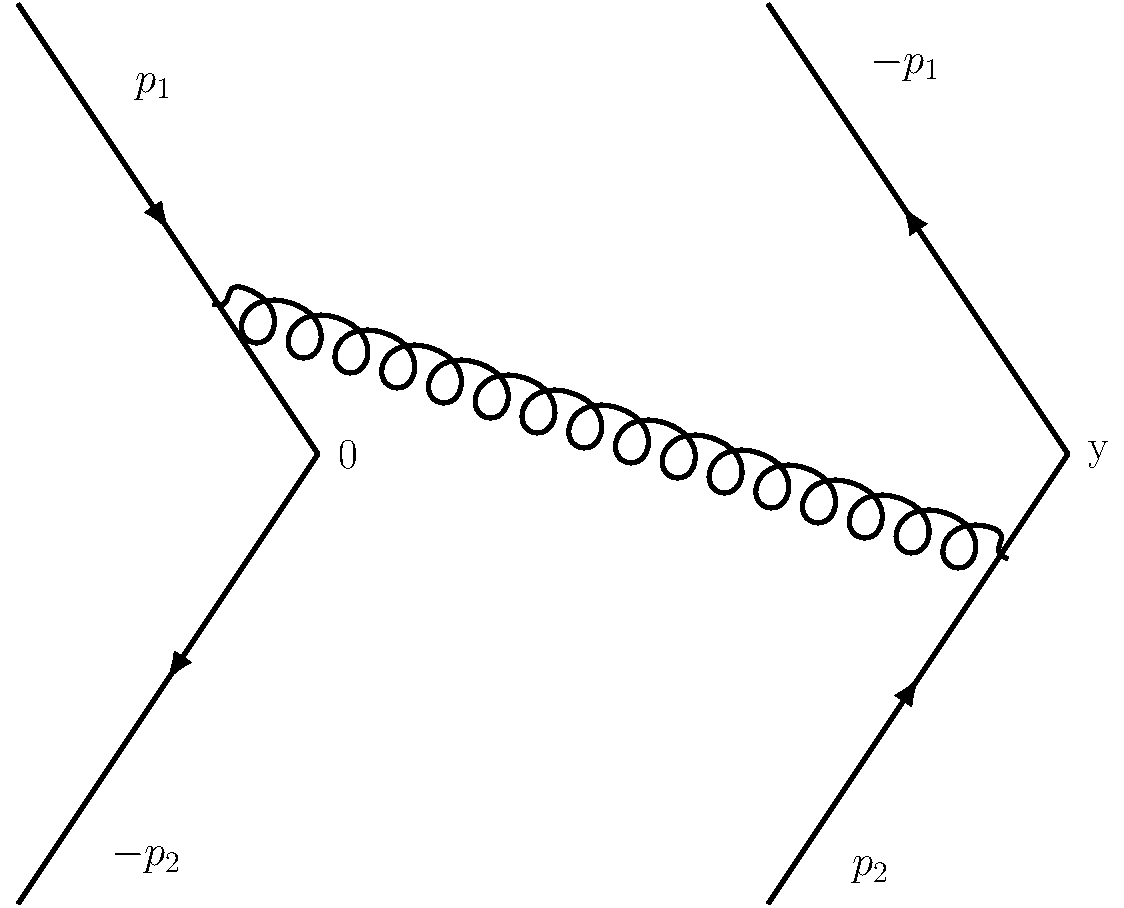
\includegraphics[scale=0.3]{Figures/DrellYanLoop.pdf}
    \caption{A one-loop contribution to the Drell-Yan eikonal cross section.}
    \label{fig:DYwilsonloopcutpropagator}
\end{figure}
%%%%%%%%%%%%%%%%%%%%%%%%%%%%%%%%%%%%%%
But before we give the procedure to find the eikonal cross section, we take a look at the structure of the expansion in \cref{eq:W(Drell) to one-loop}. We observe that the factor in front of the integral looks very much like the one-loop cusp anomalous dimension in \cref{eq:one-loop cusp anomalous dimension}. So if we use that the scale of the coupling is $\alpha_{s}(k_{\perp})$, we can write the expansion as\footnote{It is understood that it is the cusp anomalous dimension for particles in the fundamental representation.}
\begin{align}\label{eq:W(Drell) to one-loop number two}
    \mathcal{W}_{DY}&=1+\int\frac{d^{2-2\epsilon}k_{\perp}}{(2\pi)^{1-2\epsilon}}\Gamma_{\text{cusp}}(\alpha_{s}(k_{\perp}))\int dk^{+}dk^{-}\,\delta(2k^{+}k^{-}-k_{\perp}^{2})\frac{(e^{-iy^{0}(k^{+}+k^{-})/\sqrt{2}}-1)}{k^{+}k^{-}}\,,
\end{align}
where we have inserted for $d=4-2\epsilon$ and it is understood that one has to use the running coupling at one-loop order, e.g. the one-loop in \cref{eq:one-loop strong coupling}. Further, by using the non-Abelian exponentiation theorem we can write $\mathcal{W}_{DY}$ as
\begin{align}\label{eq:relation wDY and WDY}
    \mathcal{W}_{DY}=1+\sum_{n=1}^{\infty}\mathcal{W}_{DY}^{(n)}=\exp\Big(\sum_{n=1}^{\infty}W_{DY}^{(n)}\Big)\,,
\end{align}
where $W_{DY}$ are the webs we alluded to in \cref{sec:exponentiation}\footnote{For more details on webs, see \cite{White:2015wha,article}.}. For Drell-Yan, we have that $\mathcal{W}_{DY}^{(1)}=W_{DY}^{(1)}$, which we will use for our calculation. This is not true in general, but we are only interested in the one-loop result.

From the non-Abelian eikonal exponentiation theorem, the Mellin transformed eikonal cross section can on the most general form be written as \cite{laenen2000power}\footnote{The expression in \cite{laenen2000power} is for joint resummation, i.e. threshold and low transverse momentum of the final state. We are only considering threshold resummation, so we adjust the expression to our purpose.}
\begin{align}\label{eq:general result of eikonal cross section}
    \Me{\sigma}_{ij}^{\text{(eik)}}(N,Q,\epsilon)=\exp\Big(&2\int\frac{d^{4-2\epsilon}k}{\Omega_{1-2\epsilon}}\,\theta\Big(\frac{Q}{\sqrt{2}}-k^{+}\Big)\theta\Big(\frac{Q}{\sqrt{2}}-k^{-}\Big)\nonumber
    \\
    &W_{DY}\big(k^{2},\frac{n_{1}\cdot k\,n_{2}\cdot k}{n_{1}\cdot n_2},\mu,\alpha_{s},\epsilon\big)\Big(e^{-Nk^{0}/Q}-1\Big)\Big)\nonumber
    \\
    &=\exp\big(\Me{E}^{\text{(eik)}}(N,\epsilon)\big)\,,
\end{align}
where $W_{DY}$ is the web, and the invariance under rescaling of the momentum is applied. The theta functions are used to cut off the $k^{+}$ and $k^{-}$ integrals such that they are UV-finite and resctricts the $k_{\perp}$ integral to have the maximum value of $Q^{2}$. Without this restriction, the exponentiation conditions would not be valid \cite{Laenen:2004pm}. The appearance of $N$ in the exponent can be understood from the taking the Mellin transform of \cref{eq:order g2 DY wilson loop}, using the saddle point approximation $y^{0}\approx -iN/Q$ as discussed in \cite{KORCHEMSKY1993433}. The angular factor can in $d$-dimension be found in \cref{eq:d-dimensional sphere area}. 

We can now use that $W_{DY}^{(1)}=\mathcal{W}_{DY}^{(1)}$, and use \cref{eq:W(Drell) to one-loop number two} to write the exponent as
\begin{align}
    \Me{E}^{\text{(eik)}}(N,Q,\epsilon)&=2\int\frac{d^{2-2\epsilon}k_{\perp}}{\Omega_{1-2\epsilon}}\Gamma_{\text{cusp}}(\alpha_{s}(k_{\perp}))\int dk^{+}dk^{-}\,\theta\Big(\frac{Q}{\sqrt{2}}-k^{+}\Big)\theta\Big(\frac{Q}{\sqrt{2}}-k^{-}\Big)\nonumber
    \\
    &\hspace{2cm}\times\delta(2k^{+}k^{-}-k_{\perp}^{2})\frac{1}{k^{+}k^{-}}\big(e^{-N(k^{+}+k^{-})/\sqrt{2}Q}-1\big)\nonumber
    \\
    &=4\int\frac{d^{2-2\epsilon}k_{\perp}}{\Omega_{1-2\epsilon}}\frac{\Gamma_{\text{cusp}}(\alpha_{s}(k_{\perp}))}{k_{\perp}^{2}}\int\frac{dk^{+}}{2k^{+}}\,\theta\Big(\frac{Q}{\sqrt{2}}-k^{+}\Big)\theta\Big(\frac{Q}{\sqrt{2}}-\frac{k_{\perp}^{2}}{2k^{+}}\Big)\nonumber
    \\
    &\hspace{2cm}\times\Big(e^{-N\big(k^{+}+\frac{k_{\perp}^{2}}{2k^{+}}\big)/\sqrt{2}Q}-1\Big)
\end{align}
where we have applied the delta function over $k^{-}$. Because of the theta functions, the lower and upper limits of the $k^{+}$ integral are finite. Hence, the exponent take the form 
\begin{align}
    \Me{E}^{\text{(eik)}}(N,Q,\epsilon)&=4\int\frac{d^{2-2\epsilon}k_{\perp}}{\Omega_{1-2\epsilon}}\frac{\Gamma_{\text{cusp}}(\alpha_{s}(k_{\perp}))}{k_{\perp}^{2}}\int_{k_{\perp}^{2}/\sqrt{2}Q}^{Q/\sqrt{2}}\frac{dk^{+}}{2k^{+}}\Big(e^{-N\big(k^{+}+\frac{k_{\perp}^{2}}{2k^{+}}\big)/\sqrt{2}Q}-1\Big)\,.
\end{align}


%To treat the $k^{+}$ and $k^{-}$ integrals we will instead of using \cref{eq:k+k- relation in calculation}, use that $k^{+}k^{-}=(k^{2}+k_{\perp}^{2})/2$ which follows from \cref{App.eq:light-cone momenta squared}. Then by a change of variable using \cref{eq:minus ligh-cone momenta} and \cref{eq:energy relation lightcone momenta}, the exponent can be written as
%\begin{align}
%    \Me{E}^{\text{(eik)}}(N,Q,\epsilon)&=2\int\frac{d^{2-2\epsilon}k_{\perp}}{\Omega_{1-2\epsilon}}\int dk^{2}\int\frac{dk^{+}}{2k^{+}}\theta\Big(\frac{Q}{\sqrt{2}}-k^{+}\Big)\theta\Big(\frac{Q}{\sqrt{2}}-\frac{k_{\perp}^{2}+k^{2}}{2k^{+}}\Big)\nonumber
%    \\
%    &\hspace{1cm}W_{ij}\big(k^{2},k^{2}+k_{\perp}^{2},\mu,\alpha_{s},\epsilon\big)\Big(e^{-N\big(k^{+}+\frac{k_{\perp}^{2}+k^{2}}{2k^{+}}\big)/\sqrt{2}Q}-1\Big)\nonumber
%    \\
%    &=2\int\frac{d^{2-2\epsilon}k_{\perp}}{\Omega_{1-2\epsilon}}\int_{0}^{Q^{2}-k_{\perp}^{2}} dk^{2}\,W_{ij}\big(k^{2},k^{2}+k_{\perp}^{2},\mu,\alpha_{s},\epsilon\big)\nonumber
%    \\
%    &\hspace{0.5cm}\int_{(k_{\perp}^{2}+k^{2})/\sqrt{2}Q}^{Q/\sqrt{2}}\frac{dk^{+}}{2k^{+}}\Big(e^{-N\big(k^{+}+\frac{k_{\perp}^{2}+k^{2}}{2k^{+}}\big)/\sqrt{2}Q}-1\Big)\,,
%\end{align}
%where the theta functions has acted to give finite limits to the $k^{2}$ and $k^{+}$ integrals. If that step is not obvious, set the upper limit of $k^{+}=Q/\sqrt{2}$ inside the other step function and solve for $k^{2}$, giving $k^{2}=Q^{2}-k_{\perp}^{2}$. Similarly for the lower bound of $k^{+}$.

One of the $k^{+}$ integrals are straightforward, i.e.
\begin{align}
    \int_{k_{\perp}^{2}/\sqrt{2}Q}^{Q/\sqrt{2}}\frac{dk^{+}}{2k^{+}}=-\ln\Big(\sqrt{\frac{k_{\perp}^{2}}{Q^{2}}}\Big)\,,
\end{align}
while the other is more tricky, it can be shown that for large $N$ this behaves as a zeroth order modified bessel function of the second kind
\begin{align}
    K_{0}(z)=\int_{0}^{\infty}\frac{dt}{2t}e^{-t-\frac{z^{2}}{4t}}\,.
\end{align}

The actual rewriting is not pretty, but with a change of variable $t=Nk^{+}/\sqrt{2}Q$, this integral can in the large $N$ limit be represented as
\begin{align}
    \int_{k_{\perp}^{2}/\sqrt{2}Q}^{Q/\sqrt{2}}\frac{dk^{+}}{2k^{+}}\,e^{-N\big(k^{+}+\frac{k_{\perp}^{2}}{2k^{+}}\big)/\sqrt{2}Q}=K_{0}\Big(2N\sqrt{\frac{k_{\perp}^{2}}{Q^{2}}}\Big)\,,
\end{align}
up to terms of $\mathcal{O}(e^{-N})$.

After these considerations, we can write the exponent as
\begin{align}\label{eq:med eiko exponent}
   \Me{E}^{\text{(eik)}}(N,Q,\epsilon)&=4\int\frac{d^{2-2\epsilon}k_{\perp}}{\Omega_{1-2\epsilon}}\frac{\Gamma_{\text{cusp}}(\alpha_{s}(k_{\perp}))}{k_{\perp}^{2}}\,\Big[K_{0}\Big(2N\sqrt{\frac{k_{\perp}^{2}}{Q^{2}}}\Big)+\ln\Big(\sqrt{\frac{k_{\perp}^{2}}{Q^{2}}}\Big)\Big]\,.
\end{align}
We observe that the logarithm inside the bracket is divergent for $k_{\perp}\rightarrow 0$, but if we use the following expansion of the bessel function for $z$ small
\begin{align}
    K_{0}(z)=-\ln\big(\frac{ze^{\gamma_{E}}}{2}\big)-\frac{z^{4}}{4}\big[\ln\big(\frac{ze^{\gamma_{E}}}{2}\big)-1\big]+\mathcal{O}(z^{4})\,,
\end{align}
and only keep the first term, we see that the term inside the bracket in \cref{eq:med eiko exponent} is given by
\begin{align}
    K_{0}\Big(2N\sqrt{\frac{k_{\perp}^{2}}{Q^{2}}}\Big)+\ln\Big(\sqrt{\frac{k_{\perp}^{2}}{Q^{2}}}\Big)&\approx -\ln\bar{N}-\ln\Big(\sqrt{\frac{k_{\perp}^{2}}{Q^{2}}}\Big)+\ln\Big(\sqrt{\frac{k_{\perp}^{2}}{Q^{2}}}\Big)\nonumber
    \\
    &=-\ln\bar{N}\,,
\end{align}
i.e. the logarithm that diverges for $k_{\perp}\rightarrow 0$ cancels in the sum. There is still a collinear divergences, but we will soon see how to treat it.   





%To proceed from here there are some general considerations about the renormalization properties of webs that can be used, see \cite{Berger_2002,laenen2000power}. But we choose the less general path and just consider the one-loop calculation. We have partially performed the calculation of $W_{\text{DY}}^{(1)}$, so if we look at the structure of \cref{eq:W(Drell) to one-loop number two} and use the relation in \cref{eq:relation wDY and WDY}, the exponent can be written on the form
%\begin{align}
%    \Me{E}_{ij}^{\text{(eik)}}(N,Q,\epsilon)&=4\int\frac{d^{2-2\epsilon}k_{\perp}}{\Omega_{1-2\epsilon}}\frac{\Gamma_{\text{cusp}}^{(i)}(\alpha_{s}(k_{\perp}))}{k_{\perp}^{2}}\nonumber
%    \\
%    &\hspace{1cm}\int_{0}^{Q^{2}-k_{\perp}^{2}}dk^{2}\,\Big(K_{0}\Big(2N\sqrt{\frac{k_{\perp}^{2}+k^{2}}{Q^{2}}}\Big)+\ln\Big(\sqrt{\frac{k_{\perp}^{2}+k^{2}}{Q^{2}}}\Big)\Big)\,.
%\end{align}
%We can observe that for $k^{2}+k_{\perp}^{2}\rightarrow 0$ the logarithm diverges. However, the bessel function has the expansion for low $z$
%\begin{align}
%    K_{0}(z)=-\ln\big(\frac{ze^{\gamma_{E}}}{2}\big)-\frac{z^{4}}{4}\big[\ln\big(\frac{ze^{\gamma_{E}}}{2}\big)-1\big]+\mathcal{O}(z^{4})\,,
%\end{align}
%and by keeping only the first term in this expansion, the sum inside the bracket will in this limit take the form
%\begin{align}
%    K_{0}\Big(2N\sqrt{\frac{k_{\perp}^{2}+k^{2}}{Q^{2}}}\Big)+\ln\Big(\sqrt{\frac{k_{\perp}^{2}+k^{2}}{Q^{2}}}\Big)&\approx -\ln\bar{N}-\ln\Big(\sqrt{\frac{k_{\perp}^{2}+k^{2}}{Q^{2}}}\Big)+\ln\Big(\sqrt{\frac{k_{\perp}^{2}+k^{2}}{Q^{2}}}\Big)\nonumber
%    \\
%    &=-\ln\bar{N}\,,
%\end{align}
%and thus the divergence of the $k^{2}$ integral is effectively canceled in the sum. The rest of the integral over $k^{2}$ will give terms that are finite. These are not of leading logarithmic order, so we collect them in a function $B(Q,k_{\perp},\alpha_{s}(k_{\perp}))$. 

To further rewrite the expoenent, we set $\epsilon=0$ and use that the theta functions in \cref{eq:general result of eikonal cross section} restricts the $k_{\perp}$ integral to maximum value of $Q
^{2}$\footnote{This had to be true for the exponentiation conditions to be valid.}. By using polar coordinates $d^{2}k_{\perp}=k_{\perp}dk_{\perp}d\Omega_{1}$, we can write
\begin{align}
    \int\frac{d^{2}k_{\perp}}{\Omega_{1}}=\frac{1}{2}\int_{0}^{Q^{2}}dk_{\perp}^{2}\,,
\end{align}
and we arrive at the result
\begin{align}
    \Me{E}_{ij}^{\text{(eik)}}(N,\epsilon)=&2\int_{0}^{Q^{2}}\frac{dk_{\perp}^{2}}{k_{\perp}^{2}}\Gamma_{\text{cusp}}^{(i)}(\alpha_{s}(k_{\perp}))\Big[K_{0}\big(2N\frac{k_{\perp}}{Q}\big)+\ln(\frac{k_{\perp}}{Q})\big)\Big]\,,
\end{align}
which is only valid up to large logarithms. 

The eikonal cross section in \cref{eq:general result of eikonal cross section} can then be written as
\begin{align}
    \Me{\sigma}_{ij}^{\text{(eik)}}(N,Q,\epsilon)=\exp\Big(2\int_{0}^{Q^{2}}\frac{dk_{\perp}^{2}}{k_{\perp}^{2}}\Gamma_{\text{cusp}}^{(i)}(\alpha_{s}(k_{\perp}))\Big[K_{0}\big(2N\frac{k_{\perp}}{Q}\big)+\ln(\frac{k_{\perp}}{Q})\Big]\Big)\,.
\end{align}

As previously mentioned there is still a collinear divergence in this expression. However, we factorized $\Me{\sigma}_{ij}^{\text{(eik)}}(N,\epsilon)$ in such a way that $\Me{w}_{ij}^{\text{(eik)}}(N)$ was to be free of these divergences. Hence, by using \cref{eq:eikonal approcximation of partonic} we divide by the eikonal parton distributions \cref{eq:RGE parton in parton eikonal}
\begin{align}
    \Me{w}_{ij}^{\text{(eik)}}(N,Q,\mu,\alpha_s)=\frac{\Me{\sigma}_{ij}^{\text{(eik)}}(N,Q,\epsilon)}{\tilde{f}_{i/i}^{\text{(eik)}}(N,\mu,\epsilon)\tilde{f}_{j/j}^{\text{(eik)}}(N,\mu,\epsilon)}\,,
\end{align}
giving the exponent
\begin{align}
    \hat{\Me{E}}_{ij}^{\text{(eik)}}(N,Q,\mu)=&2\int_{0}^{Q^{2}}\frac{dk_{\perp}^{2}}{k_{\perp}^{2}}\Gamma_{\text{cusp}}^{(i)}(\alpha_{s}(k_{\perp}))\Big[K_{0}\big(2N\frac{k_{\perp}}{Q}\big)+\ln(\frac{k_{\perp}}{Q})\Big]\nonumber
    \\
    &+2\int_{0}^{\mu^{2}}\frac{d\mu'^{2}}{\mu'^{2}}\Gamma_{\text{cusp}}^{(i)}(\alpha_{s}(\mu'))\ln\bar{N}\,.
\end{align}

If we add $(\ln\bar{N}-\ln\bar{N})$ inside the bracket of the first line and choose $\mu'=k_{\perp}$, we can group these terms as
\begin{align}
    \hat{\Me{E}}_{ij}^{\text{(eik)}}(N,Q,\mu)=&2\int_{0}^{Q^{2}}\frac{dk_{\perp}^{2}}{k_{\perp}^{2}}\Gamma_{\text{cusp}}^{(i)}(\alpha_{s}(k_{\perp}))\Big[K_{0}\big(2N\frac{k_{\perp}}{Q}\big)+\ln(\bar{N}\frac{k_{\perp}}{Q})\Big]\nonumber
    \\
    &-2\int_{\mu^{2}}^{Q^{2}}\frac{dk_{\perp}^{2}}{k_{\perp}^{2}}\Gamma_{\text{cusp}}^{(i)}(\alpha_{s}(k_{\perp}))\ln\bar{N}\,,
\end{align}
and by choosing $\mu=Q$ can remove the last term. Hence, the eikonal function is given by
\begin{align}\label{eq:final result eikonal hard function}
    \Me{w}_{ij}^{\text{(eik)}}(N,Q,\mu,\alpha_s)=\exp\Big(2\int_{0}^{Q^{2}}\frac{dk_{\perp}^{2}}{k_{\perp}^{2}}\Gamma_{\text{cusp}}^{(i)}(\alpha_{s}(k_{\perp}))\Big[K_{0}\big(2N\frac{k_{\perp}}{Q}\big)+\ln(\bar{N}\frac{k_{\perp}}{Q})\Big]\Big)\,,
\end{align}
and we can see that when $k_{\perp}\rightarrow 0$ the integral is finite as the bracket perfectly cancels.

We should mention that in the general treatment, one should keep the distinction between the renormalization scale $\mu$, factroization scale $\mu_{F}$ and $Q$. But for simplicity we have chosen them all to be the same.  


\section{Logarithmic Corrections in Drell-Yan}
In this section we will use \cref{eq:final result eikonal hard function} to show how we can reproduce the large logarithm found in the NLO calculation \cref{eq:Mellin space NLO of omegaqbarq}, and also show that we find higher order logartithms without doing any higher order loop calculations. 

For the current discussion we are only interested in the large logarithmic corrections, so we neglect $H(Q,\alpha_s)$ in \cref{eq:partonic and eikonal relation}\footnote{From factorization theorems this does not include logarithmic corrections.}. Then from \cref{eq:final result eikonal hard function} it follows that the partonic function $\Me{w}_{q\bar{q}}$ has exponentiated, i.e
\begin{align}
    \Me{w}_{q\bar{q}}(N,Q,\alpha_{s}(Q))=\exp\Big(2\int_{0}^{Q^{2}}\frac{dk_{\perp}^{2}}{k_{\perp}^{2}}\Gamma_{\text{cusp}}^{(q)}(\alpha_{s}(k_{\perp}))\Big[K_{0}\big(2N\frac{k_{\perp}}{Q}\big)+\ln(\bar{N}\frac{k_{\perp}}{Q})\Big]\Big)\,.
\end{align}
The lower limit does not give a well defined result, but to produce large logarithms it is standard to evaluate these from $Q^{2}/\bar{N}$ up to $Q^{2}$ \cite{KORCHEMSKY1993433}\footnote{They actually solve a renormalization group equation for the Wilson line, where the integral is evaluated from $Q^{2}/\bar{N}$ up to $Q^{2}$.}. We can justify this by the approximation $Q^{2}/N\approx 0$ as $N\rightarrow\infty$. With this change of lower limit, we can make the change of variable $x=k_{\perp}/Q$, giving the exponent
\begin{align}
    \Me{E}_{q\bar{q}}(N,Q,\alpha_s)=4\int_{1/\bar{N}}^{1}\frac{dx}{x}\Gamma_{\text{cusp}}^{(q)}(\alpha_{s}(Qx))\Big[K_{0}\big(2Nx\big)+\ln(\bar{N}x)\Big]\,,
\end{align}
which can be simplified even further by looking at the large $N$ behaviour of the Bessel function. For large values of the argument, the modified Bessel function has the following expansion
\begin{align}
    K_{0}(z)=\big(\frac{\pi}{z}\Big)^{1/2}e^{-z}\big(1-\mathcal{O}(z^{-1})\big)\approx0\,,
\end{align}
and the exponent can be simplifies to
\begin{align}\label{eq:integral for drell-yan logarithms}
    \Me{E}_{q\bar{q}}(N,Q,\alpha_s)=4\int_{1/\bar{N}}^{1}\frac{dx}{x}\Gamma_{\text{cusp}}^{(q)}(\alpha_{s}(Qx))\ln(\bar{N}x)\,,
\end{align}
valid up to constant terms that are negligible in the large $N$ limit.

This integral can now be solved by using the one-loop cusp anomalous dimension \cref{eq:one-loop cusp anomalous dimension}, and the one-loop running coupling \cref{eq: g running coupling one-loop}
\begin{align}
    \Gamma_{\text{cusp}}(\alpha_{s}(Qx))&=\frac{\alpha_{s}(Qx)}{\pi}C_{F}\,,
    \\
    \alpha_{s}(Qx)&=\frac{\alpha_{s}(Q)}{1+\frac{\alpha_{s}(Q)}{2\pi}\beta_{0}\ln x}\,.
\end{align}
Inserting these expression into \cref{eq:integral for drell-yan logarithms}, and with another change of variable $y=\ln x$ gives the LL (leading logarithmic) result
\begin{align}\label{eq:LL result}
    \Me{E}_{q\bar{q}}^{(\text{LL})}(N,Q,\alpha_s)&=4\int_{1/\bar{N}}^{1}\frac{dx}{x}\frac{\alpha_{s}(Q)}{\pi}C_{F}\Big(1+\frac{\alpha_{s}(Q)}{2\pi}\beta_{0}\ln x\Big)^{-1}\ln\bar{Nx}\nonumber
    \\
    &=A_{q\bar{q}}\big[2\bar{\lambda}+(1-2\bar{\lambda})\ln(1-2\bar{\lambda}))\big]\,,
\end{align}
giving
\begin{align}\label{eq: omega LL result}
    \Me{w}_{q\bar{q}}^{(\text{LL})}(N,Q,\alpha_{s}(Q))=\exp\Big(A_{q\bar{q}}\big[2\bar{\lambda}+(1-2\bar{\lambda})\ln(1-2\bar{\lambda})\big]\Big)\,,
\end{align}
where we have defined $A_{q\bar{q}}=C_{F}/\alpha_{s}\pi b_{0}^{2}$ and $\bar{\lambda}=\alpha_s b_{0}\ln\bar{N}$, where $b_{0}=\beta_{0}/4\pi$. This result is in agreement with the LL correction for singlet ($q\bar{q}$) annihilation in Drell-Yan \cite{Catani:1996,Catani:1998}. %In order to obtain the NLL on this form we would have to use the two-loop coupling, but we will not consider that case here. 

At first sight \cref{eq: omega LL result} does not have the same form as \cref{eq:Mellin space NLO of omegaqbarq}, but if we expand the logarithm
\begin{align}
    \ln(1-2\bar{\lambda})=-2\bar{\lambda}-\bar{\lambda}^{2}-\frac{2}{3}\bar{\lambda}^{3}-\frac{1}{2}\bar{\lambda}^{4}+\cdots\,,
\end{align}
we find the LL terms
\begin{align}
    \Me{E}_{q\bar{q}}^{(\text{LL})}(N,Q,\alpha_s)=\frac{\alpha_{s}}{\pi}2C_{F}\ln^{2}\bar{N}+\Big(\frac{\alpha_{s}}{\pi}\Big)^{2}\frac{\beta_{0}}{3}C_{F}\ln^{3}\bar{N}+\Big(\frac{\alpha_{s}}{\pi}\Big)^{3}\frac{\beta_{0}^{2}}{32}\ln^{4}\bar{N}+\mathcal{O}(\alpha_{s}^{4})\,,
\end{align}
where the first term are the LL for the corresponding NLO calculation we found in \cref{eq:Mellin space NLO of omegaqbarq}\footnote{With the very important distinction that it has been exponentiated.}, and the other terms are the LL for even higher order calculations. If we wanted to compare with fixed order calculations to higher orders, we could have expanded the exponential in \cref{eq: omega LL result} and found an expanded form of $\Me{w}_{q\bar{q}}(N)$. This expansion would give fixed NLL order terms as well, but these can be found in \cite{MAGNEA1991703}. A last point to make is that in order to obtain resummed NLL terms, we would have to use the coupling to two-loop order and the cusp anomalous dimension up to two loop order, but we did not consider this scenario here.


% \section{Hadronic Cross Section and Inverse Mellin}
We have managed to bring the partonic function on an exponentiated form, but the correct observable is the hadronic cross section. So in this section we will recover the hadronic Drell-Yan cross section in $x$-space, and discuss how the inverse Mellin transform can be evaluated. 

From \cref{eq:hadronic cross section in Mellin} and \cref{eq:LL result} the Mellin transformed hadronic cross section is given by
\begin{align}
    \tilde{\sigma}_{h_1h_2}(N)&=\int_{0}^{1}d\tau \tau^{N-1}\,\frac{1}{\sigma_{0}}\frac{d\sigma_{h_1h_2}}{dQ^{2}}\nonumber
    \\
    &=\sum_{i,j=q,\bar{q}}\tilde{f}_{i/h_1}(N,Q)\tilde{f}_{j/h_2}(N,Q)\,\exp\big(\Me{E}_{ij}(N,Q,\alpha_s)\big)\,,
\end{align}
where the partonic function has been exponentiated. We can now use the inverse Mellin transform \cref{eq:Appendix Inverse Mellin} to write\footnote{Where we have recovered the fractional charge of the quarks.}
\begin{align}
    \frac{d\sigma_{h_1h_2}}{dQ^{2}}=&\,\sigma_{0}\sum_{i,j=q,\bar{q}}Q_{q}^{2}\,
    \frac{1}{2\pi i}\int_{c-i\infty}^{c+i\infty}dN\,\tau^{-N}\tilde{f}_{i/h_1}(N,Q)\tilde{f}_{j/h_2}(N,Q)\exp\big(\Me{E}_{ij}(N,Q,\alpha_s)\big)\,.
\end{align}

There exists numerical packages to evaluate parton distributions in Mellin space, see \cite{Vogt_2005}. However, the standard method is to use parton distributions sets from the LHAPDF code existing is $x$-space \cite{whalley2005les,Buckley_2015}.  To use the $x$-space formalism we can do several manipulations by using the convolution properties of the Mellin transform, given in \cref{sec:Appendix Mellin Transform}. But let us first derive an expression for the inverse Mellin transform in terms of an integral over a real variable.

\subsection{The Inverse Mellin Transform}
The inverse Mellin transform for a general function is given in terms of an integral over a complex variable $N$, see \cref{sec:Appendix Mellin Transform}, and reads
\begin{align}\label{eq:h}
    h(x)=\frac{1}{2\pi i}\int_{c-i\infty}^{c+i\infty}dN\,x^{-N}\,\Me{h}(N)\,,
\end{align}
where 
\begin{align*}
    \Me{h}(N)=\int_{0}^{\infty}dx\,x^{N-1}\,h(x)\,.
\end{align*}
Since $h(x)$ is a real valued function
\begin{align}\label{eq:h_real}
    \Me{h}^{*}(N)=\int_{0}^{\infty}dx\,x^{N^{*}-1}\,h(x)=\Me{h}(N^{*})\,.
\end{align}

The Mellin inversion integral \cref{eq:h} can be splitt in two, one part for the lower bound and one part for the upper bound. To manipulate the integral, we make a change of variable $N\rightarrow N^{*}$ in the term that is integrated from $c-i\infty$ up to $c$. This makes the integration bound change accordingly $c-i\infty\rightarrow c+i\infty$, and we find
\begin{align}
    h(x)&=\frac{1}{2\pi i}\Bigl(\int_{c-i\infty}^{c}dN\,x^{-N}\,\Me{h}(N)+\int_{c}^{c+i\infty}dN\,x^{-N}\,\Me{h}(N)\Bigr)\nonumber
    \\
    &=\frac{1}{2\pi i}\Bigl(\int_{c+i\infty}^{c}dN^{*}\,x^{-N^{*}}\,\Me{h}(N^{*})+\int_{c}^{c+i\infty}dN\,x^{-N}\,\Me{h}(N)\Bigr)\nonumber
    \\
    &=\frac{1}{2\pi i}\Bigl(-\int_{c}^{c+i\infty}dN^{*}\,x^{-N^{*}}\,\Me{h}^{*}(N)+\int_{c}^{c+i\infty}dN\,x^{-N}\,\Me{h}(N)\Bigr)\,,
    \intertext{and by choosing the parametrization of the Mellin variable to be $N=c+ze^{i\phi}$, in terms of real $z$, the integral will take the form}
    h(x)&=\frac{1}{2\pi i}\int_{0}^{\infty}dz\,\left(e^{i\phi}\,x^{-N}\Me{h}(N)-e^{-i\phi}\,x^{-N^{*}}\Me{h}^{*}(N)\right)\nonumber
    \\
    &=\frac{1}{2\pi i}\int_{0}^{\infty}dz\,2i\,\text{Im}\left(e^{i\phi}\,x^{-N}\Me{h}(N)\right)\nonumber
    \\
    &=\frac{1}{\pi}\int_{0}^{\infty}dz\,\text{Im}\left(e^{i\phi}\,x^{-N}\Me{h}(N)\right)\,,
\end{align}
where we used \cref{eq:h_real} and the relation
\begin{align*}
    \Me{h}(N)-\Me{h}^{*}(N)&=2i\,\text{Im}(\Me{h}(N))\,.
\end{align*}

Writing out the parametrization, the final integral is given by
\begin{align}\label{eq:Inversed Mellin Integral}
    h(x)=\frac{1}{\pi}\int_{0}^{\infty}dz\,\text{Im}\left(e^{i\phi}\,x^{-c-z\,\exp(i\phi)}\Me{h}(c+z\,\exp(i\phi))\right)\,.
\end{align}


\subsection{Hadronic Cross Section in $x$-space}
In order to rewrite the inverse Mellin in $x$-space it is advantageous to use that \cref{eq:Factorized Dre-Yan Cross Section} is understood to be a Mellin convolution. Let us begin with \cref{eq:Factorized Dre-Yan Cross Section}, and use \cref{eq:Appendix Mellin convolution} to write it as\footnote{For simplicity we have abbreviated some of the arguments in the integrand.}
\begin{align}
    \frac{ d\sigma_{h_1h_2}}{dQ^{2}}=\sigma_{0}\sum_{i,j=q,\bar{q}}\int_{0}^{1}dz\,dx_{1}\,dx_{2}\,\delta\big(\tau-x_{1}x_{2}z\big) f_{i/h_1}(x_1)f_{j/h_2}(x_2)\,\omega_{ij}(z)\,,
\end{align}
and using the delta function property
\begin{align}\label{eq:delta_property}
    \int dx\,\delta(g(x))=\abs{\frac{\partial g}{\partial x}}_{x=x^{*}}^{-1}\int dx\,\delta(x-x^{*})\,,
\end{align}
we find that
\begin{align}\label{eq:rewritten convolution to inverse}
    \frac{ d\sigma_{h_1h_2}}{dQ^{2}}=\sigma_{0}\sum_{i,j=q,\bar{q}}\int_{\tau}^{1}\frac{dz}{z}\int_{\tau/z}^{1}\frac{dx_1}{x_1}f_{i/h_1}(x_1)f_{j/h_2}\Big(\frac{\tau}{x_1z}\Big)\,\omega_{ij}(z)\,,
\end{align}
where the limits have changed after acting with the delta function, i.e. we have
\begin{align}
    x_{2}=\frac{\tau}{x_1z}\leq 1\,,
    \hspace{0.7cm}
    \frac{\tau}{z}\leq x_1\leq 1\,,
    \hspace{0.7cm}
    \tau\leq z\leq 1\,.
\end{align}

%Then by Parseval's convolution theorem for the inverse Mellin transform, we have that
%\begin{align}
%    \int_{\tau}^{1}\frac{dz}{z}\int_{\tau/z}^{1}\frac{dx_1}{x_1}f_{i/h_1}(x_1)f_{j/h_2}\Big(\frac{\tau}{x_1z}\Big)\,\omega_{ij}(z)=\frac{1}{2\pi i}\int_{c-i\infty}^{c+i\infty}dN\,\tau^{-N}\tilde{f}_{i/h_1}(N)\tilde{f}_{j/h_2}(N)\Me{\omega}_{ij}(N)\,,
%\end{align}
%where it follows that we can evaluate the left hand side with $x$-space parton distributions, while $\omega(z)$ is evaluated as an inverse Mellin.

To actually perform the inverse transform is a nontrivial exercise, so let us go through some of the general details. The difficulty originates from the singularity structure of the integrand. These singularities can be divided into two regions in the complex $N$-plane, see \cref{fig:MP contour}. The first ones are positioned in the left part of the complex plane. These are the result of poles in the parton distribution functions $\Me{f}_{i/h}$. In general, the functional form of parton distributions functions at the initial scale $\mu_{0}$ is given by
\begin{align}
    xf_{i/h}(x,\mu_{0})=\sum_{n}A_{n}x^{\gamma_n}(1-x)^{\delta_n}\,,
\end{align}
where $A_{n}$, $\gamma_n$ and $\delta_{n}$ are obtained from a fitting procedure to hard scattering data, and for small $x$ and $\gamma_n<0$ this becomes singular. In Mellin space, this is transformed to
\begin{align}
    \Me{f}_{i/h}(N,\mu_{0})=\sum_{n}A_{n}\beta(N+\gamma_n,1+\delta_n)\,,
\end{align}
where $\beta(a,b)$ is the Euler-beta function in which the singular behaviour is well known. This first region can be avoided by choosing the contour in \cref{fig:MP contour}, as derived in \cite{Catani:1996}. We observe that the singularities from the parton distributions are avoided by choosing a constant $C_{MP}$ that lies to the right of the rightmost singularity of $\Me{f}_{i/h}$. 

The second region is more troublesome, as it is in the right part of the complex $N$-plane. This singularity originates from the Landau pole that arises for small couplings, i.e. the non-perturbative regime of QCD. The Landau pole manifest itself in the exponent of \cref{eq:LL result}, and is due to the expression $\ln(1-2\bar{\lambda})$. Hence, for $\bar{\lambda}=1/2$ we have
\begin{align}
    N_{L}=e^{-\gamma_{E}}e^{\frac{1}{2b_{0}\alpha_s}}\,.
\end{align}

This problem has been extensively studied in the litterature, and the most common approach is the so-called \emph{Minimal Prescription} \cite{Catani:1996}. This method states that the contour has to be chosen such that the constant $C_{MP}$, satisfies
\begin{align}
    C_{f}<C_{MP}<N_{L}\,,
\end{align}
where $C_{f}$ is the rightmost pole of $\Me{f}_{i/h}$. In \cref{fig:MP contour} we see the possible contours, where $C_{0}$ is the vertical line and $C_{1}$ is the bent contour. As argued in \cite{Catani:1996}, the choice $C_{MP}=2$ and $C_1$ with $\phi >\pi/2$, will make the integral converge faster than the choice $C_{MP}=2$ and $C_{0}$ with $\phi=\pi/2$.
\begin{figure}
    \centering
    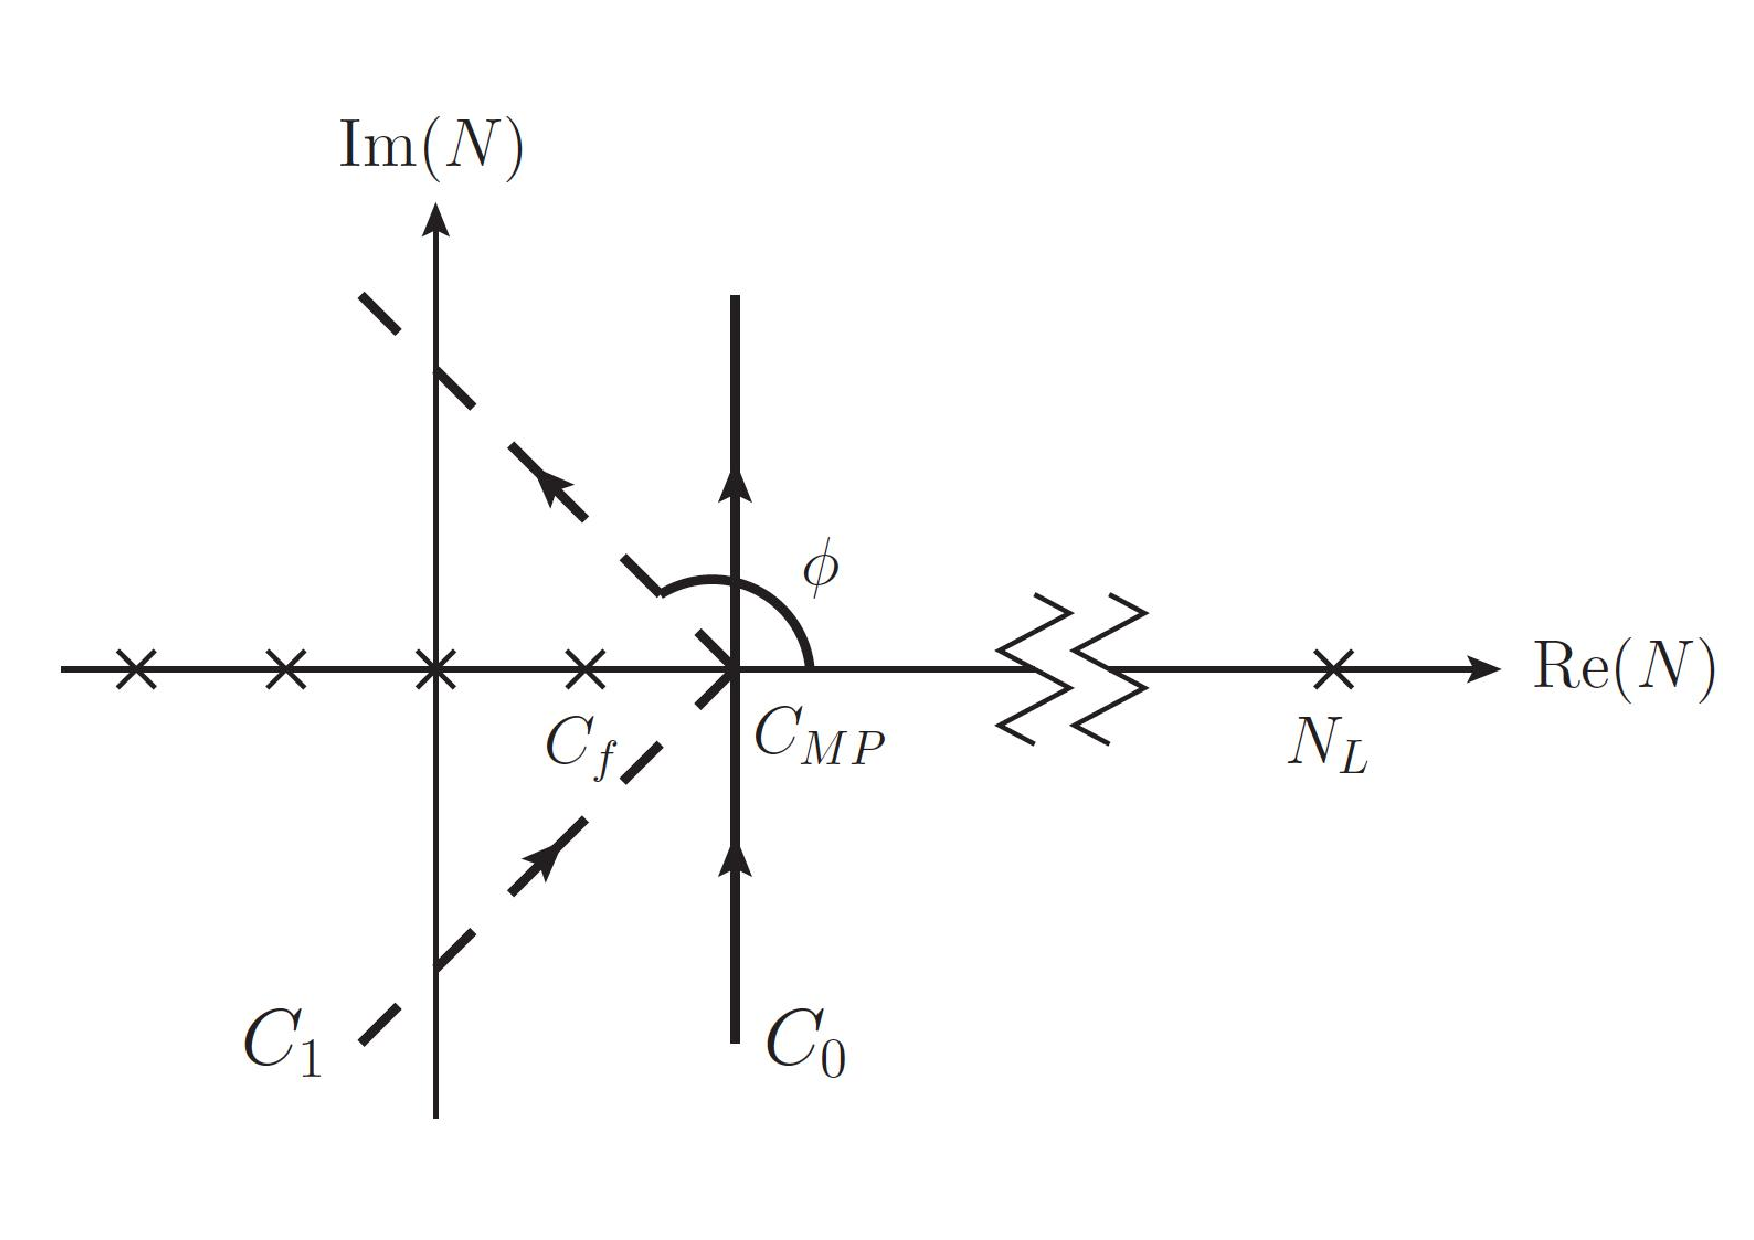
\includegraphics[scale=0.4]{Figures/CMP.pdf}
    \caption{Possibilities to choose the contour for the Mellin inversion as proposed in \cite{Catani:1996}. $C_{0}$ is the vertical contour and $C_{1}$ is the contour with an angle.}
    \label{fig:MP contour}
\end{figure}

So if the hadronic cross section is to be calculated with parton distributions in Mellin space, the following integral must be implemented
\begin{align}
    \frac{d\sigma_{h_1h_2}}{dQ^{2}}=&\,\sigma_{0}\sum_{i,j=q,\bar{q}}Q_{q}^{2}\,\frac{1}{\pi}\int_{0}^{\infty}dy\,\text{Im}\Big[e^{i\phi}\tau^{-N}\tilde{f}_{i/h_1}(N,Q)\tilde{f}_{j/h_2}(N,Q)\,\Me{\omega}_{ij}(N,\alpha_{s}(Q))\Big]\,,
\end{align}
where we used \cref{eq:Inversed Mellin Integral} to write the cross section as an integral over a real variable and $N=C_{MP}+ye^{i\phi}$. 

However, to use the $x$-space formalism the hadronic cross section is obtained by calculating
\begin{align}\label{eq:next to final hadronic}
    \frac{ d\sigma_{h_1h_2}}{dQ^{2}}=\sigma_{0}\sum_{i,j=q,\bar{q}}Q_{q}^{2}\int_{\tau}^{\infty}\frac{dz}{z}\int_{\tau/z}^{1}\frac{dx_1}{x_1}f_{i/h_1}(x_1,Q)f_{j/h_2}\Big(\frac{\tau}{x_1z},Q\Big)\,\omega_{ij}(z,Q,\alpha_{s}(Q))\,,
\end{align}
where the parton distributions are calculated in $x$-space, while the hard function is found by the inverse transform
\begin{align}
    \omega_{ij}(z,Q,\alpha_{s}(Q))=\frac{1}{\pi}\int_{0}^{\infty}dy\,\text{Im}\big(e^{i\phi}z^{-N}\,\Me{\omega}_{ij}(N,\alpha_{s}(Q))\big)\,.
\end{align}
We observe that the upper limit of the $z$ integral in \cref{eq:next to final hadronic} has changed. The reason for this change is that in the minimal prescription, the resummed cross section does not vanish for $z>1$ due to the Landau pole \cite{Catani:1996}. 

In \cref{eq:next to final hadronic}, the parton distributions are calculated in $x$-space, but there are problems that might occur in the hard function $\omega_{ij}$. Close to threshold, the resummed exponent can give large oscillations, see \cite{Catani:1996,KULESZA:2002} for more details. One possibility to dampen the oscillations is by a simple rewriting of the integrand. We do this by using \cref{eq:Appendix derivative of function}, to write
\begin{align}
    N\Me{f}_{i/h}(N)=\int_{0}^{1}dx\,x^{N-1}\mathcal{F}_{i/h}(x)\,,
\end{align}
where we used that parton distributions vanish for $x=1$, and defined
\begin{align}
    \mathcal{F}_{i/h}(x)=-x\frac{d}{dx}f_{i/h}(x)\,,
\end{align}
giving the modified hadronic cross section
\begin{align}
    \frac{ d\sigma_{h_1h_2}}{dQ^{2}}=\sigma_{0}\sum_{i,j=q,\bar{q}}Q_{q}^{2}\int_{\tau}^{1}\frac{dz}{z}\int_{\tau/z}^{1}\frac{dx_1}{x_1}\mathcal{F}_{i/h_1}(x_1,Q)\mathcal{F}_{j/h_2}\Big(\frac{\tau}{x_1z},Q\Big)\,\mathcal{S}_{ij}(z,Q,\alpha_{s}(Q))\,,
\end{align}
where
\begin{align}
    \mathcal{S}_{ij}(z,Q,\alpha_{s}(Q))=\frac{1}{2\pi i}\int_{C_{MP}}dN\,z^{-N}\frac{\Me{w}_{ij}(N,Q,\alpha_{s}(Q))}{N^{2}}\,.
\end{align}
The derivatives of the parton distributions can be performed numerically for the common sets \cite{Martin:2009,Pumplin:2002}. As mentioned the point of this rewriting is to dampen the behaviour of the exponent in $\omega_{q\bar{q}}$, but as argued in \cite{Catani:1996} gluon initiated processes should have even higher powers of $N$ as dampening factors. This would subsequently lead to higher order derivatives of the parton distributions.


 




%%%%%%%%%%%%% Conclusion %%%%%%%%%%%%%%%%%%%%%%%%%%
% \newpage
\chapter*{Conclusion}
\addcontentsline{toc}{chapter}{Conclusion} 
In this thesis we have investigated IR divergences that appear in gauge theories, focusing in particular on the non-Abelian gauge theory of QCD. For theories involving massless fields these divergences are a prominent feature, and in certain regions of phase space they give rise to large logarithmic corrections to physical observables. The main focus of interest was to investigate how Wilson lines and Wilson loops can be used to resum these large corrections such that physical observables exponentiate and prevents the invalidation of perturbative expansions.

\medskip
In \cref{chap:Intro QFT} we developed the route from Green's functions to scattering amplitudes and Feynman diagrams, before going into some detail about the basic ideas and possible ways of treating divergences using regularization and renormalization. We mainly focused on the UV region of phase space, as the IR region is studied in more detail in later chapters.
After this basic introduction to QFT in \cref{chap:Intro QFT}, we went on to look at the geometrical formulation of gauge theories in \cref{chap:Geometry of gauge theories}. From this formalism the concept of Wilson lines naturally appeared as fundamental building blocks for any gauge theory. We also discussed that from the Ambrose-Singer theorem it follows that physical observables can be constructed in terms of gauge invariant Wilson loops. This is the basis why we in later chapters use Wilson lines to construct Wilson loop expectation values, and from them eikonal cross sections. Further, by using Wilson lines we showed how one can construct the Yang-Mills Lagrangian from a purely geometrical standpoint. As we are mainly interested in scattering amplitudes, we focused on introducing the properties of piecewise linear Wilson lines. These naturally appear when high-energy particles meet at a point and annihilate or scatters of one another by exchanging a gauge boson.

\medskip
In \cref{Chap:pQCD} we first introduced the QCD Lagrangian and set the stage for perturbative calculations by discussing the property of asymptotic freedom in QCD. By using the most basic experimental setup of deep inelastic scattering, we went on and studied the important concepts of factorization both in the parton model and in QCD. We also introduced parton distribution functions, which is an essential ingredient in obtaining factorization in QCD. From there we made use of Wilson lines and how these can be used to render parton distributions gauge invariant. We also derived parton-in-parton distributions and showed how these can be defined such that they incorporate the collinear divergences appearing in the partonic cross section. The significance of this is that we can use factorization theorems to group divergences into different regions and define functions that are responsible for these. Lastly we investigated the appearance of large logarithms by doing an explicit NLO calculation of a lepton pair production via the annihilation of a quark-antiquark pair. We show that higher order corrections have a significant contribution to the hadronic cross section, implying that in order to have predictive results even higher order results had to be taken into account. We also made a numerical evaluation of the NLO hadronic cross section and compared with experimental results from CMS. This is of course nothing new, but the reason we used this process is because it is the simplest one to perform resummation with. By doing the NLO calculation we found a fixed order result we could compare with the resummed Drell-Yan cross section we aimed to calculate.

\medskip
In \cref{chap:Resummation in QCD} we started by looking at the behaviour of scattering amplitudes using the eikonal approximation, showing that in this limit the amplitude naturally factorizes into one hard and one soft regime. The crucial point of this derivation was to show that not only does the soft and hard parts decouple, but IR divergences coming from the soft part exponentiates. Close to the final state production threshold gluon radiation from the highly energetic initial state quarks are restricted to be soft. This implies that Wilson lines on linear paths can be used to describe the soft radiation. We use factorization theorems to first refactorize the partonic cross section in terms of parton-in-parton distributions that are responsible for collinear divergences. These cross sections are explicitly factorized by using Mellin space techniques. Then we defined a close to threshold cross section, which is factorized into three parts. One part that describes the hard process without large corrections, one part that describes collinear radiation and one part that contains soft wide angle radiation. The contribution from the soft function is found by taking the eikonal approximation giving an eikonal partonic cross section. This eikonal cross section is then constructed from a Wilson loop expectation value. The eikonal cross section contains both soft and collinear singularities, and again we used factorization theorems to group the collinear singularities into eikonal parton distributions and an infrared safe eikonal function. 

We then took a closer look at the renormalization properties of Wilson lines and parton-in-parton distributions in the $x\rightarrow 1$ limit. A piecewise linear Wilson line that is constructed in terms of two semi-infinite Wilson lines on linear paths with an angle between them, contains cusp divergences. By using the renormalization properties of Wilson lines we calculate the one-loop cusp anomalous dimension for Wilson lines on the light-cone. This calculation is important as we show that parton-in-parton distributions in the $x\rightarrow 1$ obey an evolution equation in terms of this cusp anomalous dimension. The cusp anomalous dimension also appears in the eikonal cross section, showing that it is an important ingredient when doing resummation with Wilson lines. From there we show how one can calculate the Wilson loop expectation value to one-loop order and use the non-Abelian eikonal exponentiation theorem to find the exponentiated eikonal cross section. As this eikonal cross section contains IR divergences, we use the eikonal distributions to find the infrared safe eikonal function. In the end we find an exponentiated partonic hard function, given in terms of an integral over the cusp anomalous dimension. We solve this integral by using the one-loop running coupling and find that the resummed expression contains an all order series of leading logarithmic terms. Hence, we have not only reproduced the large logarithm from the fixed order NLO calculation in \cref{Chap:pQCD}, but showed the appearance of higher order contributions without performing any fixed order calculation. We also discuss that these results are in accordance with results in the literature, apart from constant factors that we neglected throughout as we mainly focused on the limit of large $N$ in Mellin space.

Lastly, we reconstruct the full resummed hadronic cross section and show an explicit method of how one can go about calculating the inverse Mellin transform needed for a numerical evaluation. We discuss several important features that have to be taken into account when choosing the contour in Mellin space. By using that the cross section is a real valued function, we manipulate the inverse transform and show that it reduces to an integral over a real variable.

\medskip
As future work resummation techniques can be explored further by looking at physics beyond the Standard Model, for example in Supersymmetry. Supersymmetry is one of the most promising, and most studied theories for physics beyond the Standard Model. At the Large Hadron Collider there is an extensive search programme for such new physics phenomena. So far no supersymmetric particles have been found, but there is a need for higher order calculations for the production of these sparticles to precisely evaluate the current exclusion limits. As a natural extension to the work done here, we could look at the production of final state sleptons. Sleptons are colour neutral and will, as for the leptons studied here, not contain any final state gluon radiation. Hence, the radiation part of the process should not be any different from the one we have found in this thesis. The main difference will be that we are considering the production of massive particles and the threshold variable will be a function of the mass. Of course, we also have to take into account the interaction between the sleptons and the photon, leading to a different hard function. There are simplifications that can be made, and that is to look at degenerate masses. Another extension is to look at coloured final states, where one consider the production of squarks and gluinos. This extension is highly non-trivial as the final state will also contain gluon radiation. 
\backmatter{}
%%%%%%%%%%%%% Appendix %%%%%%%%%%%%%%%%%%%%%%%%

% \begin{appendices}
% \numberwithin{equation}{section}

% \appendix
% \chapter{Appendix A}
% \renewcommand{\thechapter}{A}
% \renewcommand{\theequation}{\thechapter.\arabic{equation}}
% \section{Light-Cone Coordinates}\label{sec:Appendix Light-cone coordinates}
Light-cone coordinates is specifically useful in high energy scattering processes where one want to decompose the momentum of the involving particles. For a general four vector $p^{\mu}$, one defines
\begin{align}
    p^{\mu}=(p^{+},p^{-},p_{\perp})\,,
\end{align}
where 
\begin{align}
    p^{+}&=\frac{1}{\sqrt{2}}(p^{0}+p^{3})
    \\
    p^{-}&=\frac{1}{\sqrt{2}}(p^{0}-p^{3})
    \\
    p_{\perp}&=(p^1,p^2)\,.
\end{align}
Scalar products are given by
\begin{align}
    p\cdot k&=p^{+}k^{-}+p^{-}k^{+}-p_{\perp}\cdot k_{\perp}
    \\
    p^{2}&=2p^{+}p^{-}-p_{\perp}^{2}\label{App.eq:light-cone momenta squared}\,,
\end{align}
where the transverse contraction $p_{\perp}\cdot k_{\perp}$ is understood from the definition of the transverse vector and must not be mistaken as the same as the four momentum contraction $p\cdot k$.
We will usually parametrize our momenta in terms of plus-components and from \cref{App.eq:light-cone momenta squared} it follows that the minus component can be written as
\begin{align}\label{eq:minus ligh-cone momenta}
    p^{-}=\frac{p^{2}+p_{\perp}^{2}}{2p^{+}}\,.
\end{align}
The $d$-dimensional Jacobian takes the form
\begin{align}
    d^{d}p=dp^{+}dp^{-}d^{d-2}p_{\perp}\,.
\end{align}

From the above relations the light-cone metric takes the form
\begin{align}
    g_{\text{LC}}^{\mu\nu}=\begin{pmatrix}
    0 & 1 & 0 & 0\\ 
    1 & 0 & 0 & 0\\
    0 & 0 & -1 & 0\\
    0 & 0 & 0 & -1\\
\end{pmatrix}\,,
\end{align}
where the index runs over $\mu=+,-,1,2$. We will elsewhere drop the subscript $\text{LC}$ as it will always be clear from the context when we are using light-cone coordinates. One can also define light-like basis vectors
\begin{align}
    n_{+}^{\mu}&=(1^{+},0^{-},0_{\perp})\,,\hspace{1cm}n_{+\,\mu}=(0^{+},1^{-},0_{\perp})\,,
    \\
    n_{-}^{\mu}&=(0^{+},1^{-},0_{\perp})\,,\hspace{1cm}n_{-\,\mu}=(1^{+},0^{-},0_{\perp})\,,
\end{align}
giving
\begin{align}
    n_{+}^{2}=0\,,\hspace{1cm}n_{-}^{2}=0\,,\hspace{1cm}n_{+}\cdot n_{-}=1\,.
\end{align}
These basis vectors project out the following components of a vector
\begin{align}
    p\cdot n_{+}=p^{-}\,,\hspace{1cm}p\cdot n_{-}=p^{+}\,.
\end{align}
We can also construct a transversal metric
\begin{align}\label{eq:trasnversal tensor}
    g_{\perp}^{\mu\nu}=g^{\mu\nu}-\big(n_{+}^{\mu}n_{-}^{\nu}+n_{+}^{\nu}n_{-}^{\mu}\big)=\begin{pmatrix}
    0 & 0 & 0 & 0\\ 
    0 & 0 & 0 & 0\\
    0 & 0 & -1 & 0\\
    0 & 0 & 0 & -1\\
\end{pmatrix}\,,
\end{align}
from which it follows that
\begin{align}
    g_{\perp}^{\mu\nu}g_{\perp\,\mu\nu}=2\,.
\end{align}
We can also define the gluon polarization sum in light-cone gauge, i.e $A^{+}=0$, as
\begin{align}\label{eq:gluon polarization sum light-cone gauge}
    \sum_{\text{pol}}\varepsilon_{\alpha}(k')\varepsilon_{\beta}^{*}(k')&=-g_{\alpha\beta}+\frac{k'_{\alpha}\,n_{-\,\beta}}{k'\cdot n_{-}}+\frac{k'_{\beta}\,n_{-\,\alpha}}{k'\cdot n_{-}}\,.
\end{align}











% \appendix
% \renewcommand{\thechapter}{B}
% \chapter{Appendix B}
% %\renewcommand{\theequation}{\thechapter.\arabic{equation}}
% \section{Dirac Gamma Matrices}\label{sec:Appendix Dirac gamma matrices}
In scattering processes Dirac gamma matrices are extremely useful for calculations. Using only the Dirac algebra and trace identities they can be eliminated completely without referring to any specific representation. The convention used in this thesis is based on \cite{pal2007representationindependent}, which we refer to for a more complete treatment of gamma matrices and spinors.

The gamma matrices are defined by satisfying the Dirac algebra\footnote{It is implicit that there is a four by four identity matrix in this equation.}
\begin{align}\label{eq:Dirac algebra}
    \{\gamma^{\mu},\gamma^{\nu}\}\equiv 2g^{\mu\nu}\,,
\end{align}
where $g^{\mu\nu}$ is the usual Minkowski metric tensor.

The hermitian conjugate of a gamma matrix is given by
\begin{align}
    \big(\gamma^{\mu}\big)^{\dagger}=\gamma^{0}\gamma^{\mu}\gamma^{0}\,.
\end{align}
From the Dirac algebra we can list some useful identities in $d$-dimensions
\begin{align}
    \gamma^{\mu}\gamma_{\mu}&=d
    \\
    \gamma^{\mu}\gamma^{\nu}\gamma_{\mu}&=(2-d)\gamma^{\nu}
    \\
    \gamma^{\mu}\gamma^{\nu}\gamma^{\lambda}\gamma_{\mu}&=4g^{\nu\lambda}+(d-4)\gamma^{\nu}\gamma^{\lambda}
    \\
    \gamma^{\mu}\gamma^{\nu}\gamma^{\lambda}\gamma^{\rho}\gamma_{\mu}&=(d-4)\gamma^{\nu}\gamma^{\lambda}\gamma^{\rho}-2\gamma^{\rho}\gamma^{\lambda}\gamma^{\nu}\,.
\end{align}
The trace over an odd number of gamma matrices always vanish, and for two and four gamma matrices we have the following identities
\begin{align}
    \text{tr}(\gamma^{\mu})&=0
    \\
    \text{tr}(\gamma^{\mu}\gamma^{\nu})&=4g^{\mu\nu}
    \\
    \text{tr}(\gamma^{\mu}\gamma^{\nu}\gamma^{\lambda}\gamma^{\rho})&=4\big(g^{\mu\nu}g^{\lambda\rho}-g^{\mu\lambda}g^{\nu\rho}+g^{\mu\rho}g^{\nu\lambda}\big)\,.
\end{align}
Often we will have contraction involving the Dirac slash notation $\slashed{p}=p_{\mu}\gamma^{\mu}$. In $d=4$ we have the following identities
\begin{align}
    \gamma^{\mu}\slashed{p}&=2p^{\mu}-\slashed{p}\gamma^{\mu}
    \\
    \gamma^{\mu}\slashed{p}\gamma_{\mu}&=-2\slashed{p}
    \\
    \gamma^{\mu}\slashed{p}\slashed{k}\gamma_{\mu}&=4p\cdot k
    \\
    \gamma^{\mu}\slashed{p}\slashed{k}\slashed{q}\gamma_{\mu}&=-2\slashed{p}\slashed{k}\slashed{q}\,.
\end{align}
Products of slashed vectors are given by
\begin{align}
    \slashed{p}\slashed{p}&=p^{2}
    \\
    \slashed{p}\slashed{k}\slashed{p}&=2p\cdot k\slashed{p}-p^{2}\slashed{k}
    \\
    \slashed{p}\slashed{k}\slashed{q}\slashed{p}&=2p\cdot q\slashed{p}\slashed{k}-2p\cdot k\slashed{p}\slashed{q}+p^{2}\slashed{k}\slashed{q}
    \\
    \slashed{p}\slashed{k}+\slashed{k}\slashed{p}&=2p\cdot k
    \\
    \slashed{p}\slashed{k}\slashed{q}+\slashed{q}\slashed{k}\slashed{p}&=2k\cdot q\slashed{p}-2p\cdot q\slashed{k}+2p\cdot k\slashed{q}\,.
\end{align}
One combination that occurs often in scattering amplitudes is the following trace
\begin{align}\label{eq:common trace in scattering}
    \text{tr}[\slashed{p}\gamma^{\mu}\slashed{k}\gamma^{\nu}]=4(p^{\mu}k^{\nu}+p^{\nu}k^{\mu}-g^{\mu\nu}p\cdot k)\,.
\end{align}

% \appendix
% \renewcommand{\thechapter}{C}
% \chapter{Appendix C}
% \renewcommand{\theequation}{\thechapter.\arabic{equation}}
% \section{Plus Distributions}\label{sec:Appendix Plus Distributions}
The plus distribution is a vital mathematical construct that is widely used in both fixed order and resummation calculations. On the most general form, a plus distribution is defined as
\begin{align}
    f_{+}(x)\equiv\lim_{\alpha\rightarrow 0}\Big(f(x)\theta(1-\alpha-x)-\delta(1-\alpha-x)\int_{0}^{1-\alpha}dy\,f(y)\Big)\,,
\end{align}
where $f(x)$ is singular for $x=1$. It is a distribution, so it is meant to act inside integrals. Hence, integrated with an analytic function on the domain $x\in[0,1]$, it works as
\begin{align}\label{eq:plus distribution convolution}
    \int_{0}^{1}dx\,f_{+}(x)g(x)=\int_{0}^{1}dx\,f(x)(g(x)-g(1))\,,
\end{align}
and has the useful property
\begin{align}\label{eq:plus distribution integrated over unity}
    \int_{0}^{1}dx\,f_{+}(x)=0\,.
\end{align}

In the case where the lower limit is not zero, this is evaluated as
\begin{align}
    \int_{z}^{1}dx\,f_{+}g(x)=\int_{0}^{1}dx\,f(x)(g(x)-g(1))+g(1)\ln(1-x)\,.
\end{align}

These are general considerations, but let us look at a specific case we use in this thesis. In dimensional regularization, we often encounter terms like
\begin{align}
    (1-x)^{-1-\epsilon}\,,
\end{align}
which diverges in the limit where $z\rightarrow 1$ and $\epsilon\rightarrow 0$. But the perturbative calculable functions are not the observables we are studying directly. We are integrating perturbative functions with analytic parton distribution functions, which allows us to do several manipulations. The integrals we encounter are
\begin{align}
    \mathcal{I}(x,\epsilon)=\int_{0}^{1}dx\,g(x)(1-x)^{-1-\epsilon}\,,
\end{align}
and as long as $g(x)$ does not converge towards $\mathcal{O}(1-z)$ near $z=1$ this diverges. To treat this we simply add zero to the integral in the following way
\begin{align}
    \mathcal{I}(x,\epsilon)=\int_{0}^{1}dx\,g(1)(1-x)^{-1-\epsilon}+\int_{0}^{1}dx\,\big(g(x)-g(1)\big)(1-x)^{-1-\epsilon}\,.
\end{align}
and use the beta integral to write
\begin{align}
    \int_{0}^{1}dx\,(1-x)^{-1-\epsilon}=-\frac{1}{\epsilon}\,,
\end{align}
giving the expansion in $\epsilon$
\begin{align}
    \mathcal{I}(x,\epsilon)=-\frac{1}{\epsilon}g(1)+\int_{0}^{1}dx\,\big(g(x)-g(1)\big)\Big[\frac{1}{1-z}-\frac{\ln(1-z)}{1-z}\epsilon+\mathcal{O}(\epsilon^{2})\Big]\,.
\end{align}
If we use \cref{eq:plus distribution convolution}, we have that
\begin{align}
    \mathcal{I}(x,\epsilon)=\int_{0}^{1}dx\,g(x)\Big[-\frac{1}{\epsilon}\delta(1-x)+\frac{1}{1-z}_{+}-\epsilon\Big(\frac{\ln(1-z)}{1-z}\Big)_{+}+\mathcal{O}(\epsilon^{2})\Big]\,.
\end{align}

% \appendix
% \renewcommand{\thechapter}{D}
% \chapter{Appendix D}
% \renewcommand{\theequation}{\thechapter.\arabic{equation}}
% \section{The Mellin Transform}\label{sec:Appendix Mellin Transform}
For a function $f(x)$ defined on the positive real axis, the Mellin transformation $\mathcal{M}$ is the operation mapping $f$ into the function $\Me{f}$ defined on the complex plane. It has the following definition
\begin{align}
    \mathcal{M}\big[f(x):N\big]=\tilde{f}(N)=\int_{0}^{\infty}dx\,x^{N-1}\,f(x)\,,
\end{align}
where $\Me{f}(N)$ is the Mellin transform of $f(x)$, and $N$ is the Mellin moment conjugate to $x$. In general, the integral does not exist for all functions, i.e. all functions does not have a well defined Mellin transform. But even if the transform exist, it is not guaranteed to converge. The domain of $N$ for which the integral converge for a given function is known as the fundamental strip. For a real function, the fundamental strip is denoted as $<a,b>$, given by all points on the domain $a<s<b$ such that $N=s+it$, for any t. The values of $a$ and $b$ is found by the asymptotic behaviour
\begin{align}
    a:\hspace{0.5cm}\lim_{x\rightarrow 0^{+}}f(x)&=\mathcal{O}(x^{-a})\,,
    \\
    b:\hspace{0.5cm}\lim_{x\rightarrow\infty}f(x)&=\mathcal{O}(x^{-b})\,,
\end{align}
which implies that a function defined on the domain $0<x<1$, have a fundamental strip $<a,\infty>$.

The Mellin transform is closely related to the two-sided Laplace transform, with the difference of a variable change $x\rightarrow -\ln x$. Hence, the inverse Mellin is given by
\begin{align}\label{eq:Appendix Inverse Mellin}
    \mathcal{M}^{-1}\big[\Me{f}(N):x\big]=\frac{1}{2\pi i}\int_{c-i\infty}^{c+i\infty}dN\,x^{-N}\Me{f}(N)\,,
\end{align}
where the integration contour is along a vertical line through $Re(N)=c$, as long as $c$ lies in the fundamental strip of the function. If the function is holomorphic in the strip and vanishes sufficiently fast when $Im(N)\rightarrow\pm\infty$, it follows from Cauchy's theorem that the contour may be deformed as long as no poles are crossed. 

One very important property of the Mellin transform is its effect on convolutions
\begin{align}\label{eq:Appendix Mellin convolution}
    \big(f\star g\big)(x)=\int_{0}^{1}dx_1\int_{0}^{1}dx_2\,f(x_1)g(x_2)\delta(x-x_1x_2)=\int_{x}^{1}\frac{dx_1}{x_1}\,f(x_1)g\big(\frac{x_2}{x_1}\big)\,,
\end{align}
where $x\in(0,1)$. To disentangle this convolution, one performs the transform
\begin{align}\label{eq:Appendix Mellin convolution transform}
    \mathcal{M}\big[\big(f\star g\big)(x):N\big]&=\int_{0}^{1}dx\,x^{N-1}\int_{0}^{1}dx_1\int_{0}^{1}dx_2\,f(x_1)g(x_2)\delta(x-x_1x_2)\nonumber
    \\
    &=\int_{0}^{1}dx_1\,x_1^{N-1}f(x_1)\int_{0}^{1}dx_2\,x_2^{N-1}g(x_2)\nonumber
    \\
    &=\Me{f}(N)\Me{g}(N)\,,
\end{align}
where the convolution in $x$-space has transformed into simple products in Mellin space. 

\subsection{Mellin Transforms of Functions}
This section is intended to demonstrate some of the Mellin transforms that are encountered in this thesis. Since the main focus is in the domain of large $N$, this will not be the general treatment of these transforms.

The simplest case is the Mellin transform of a constant $c$,
\begin{align}
    \int_{0}^{1}dx\,x^{N-1}c=\frac{c}{N}\,,
\end{align}
and a monomial
\begin{align}
    \int_{0}^{1}dx\,x^{N-1}x^{a}=\frac{1}{N+a}\,,
\end{align}
which combined with a logarithm
\begin{align}
    \int_{0}^{1}dx\,x^{N-1}(-x^{a}\ln x)&=-\frac{x^{N+a}}{N+a}\ln x\big|_{0}^{1}+\int_{0}^{1}dx\,\frac{x^{N+a-1}}{N+a}\nonumber
    \\
    &=\frac{1}{(N+a)^{2}}\,,
\end{align}
which can be generalized for any polynomial $P(x)$
\begin{align}
    \int_{0}^{1}dx\,x^{N-1}P(x)=\mathcal{O}(1/N)\,.
\end{align}
Furthermore, by using that $x^{N-1}=e^{(N-1)\ln x}$, repeated derivatives with respect to $N$ will give
\begin{align}
    \int_{0}^{1}dx\,x^{N-1} f(x)\ln^{k}x=\frac{d^{k}}{dN^{k}}\Me{f}(N),\hspace{1cm}\forall\,k>0\,.
\end{align}
Another useful property involves the derivative of a function
\begin{align}\label{eq:Appendix derivative of function}
    \int_{0}^{1}dx\,x^{N-1}\Big(-x\frac{d}{dx}f(x)\Big)&=-x^{N}f(x)\big|_{0}^{1}+N\int_{0}^{1}dx\,x^{N-1}f(x)\nonumber
    \\
    &=-f(1)+N\Me{f}(N)\,,
\end{align}
which is especially useful for functions that vanish for $x=1$.

The Mellin transform of plus distributions are more complicated. By using \cref{eq:plus distribution convolution}, we can write
\begin{align}
    \int_{0}^{1}dx\,x^{N-1}\Big[\frac{1}{1-x}\Big]_{+}=\int_{0}^{1}dx\Big(\frac{x^{N-1}}{1-x}-\frac{1}{1-x}\Big)\,.
\end{align}
The terms on the $rhs$ diverge when considered separately, so we can not calculate them independently. By introducing a regulator $\epsilon$, this can be rewritten by using beta integrals
\begin{align}
    \int_{0}^{1}dx \frac{x^{N-1}}{(1-x)^{1-\epsilon}}-\int_{0}^{1}dx\frac{1}{(1-x)^{1-\epsilon}}=\frac{\Gamma(N)\Gamma(\epsilon)}{\Gamma(N+\epsilon)}-\frac{\Gamma(1)\Gamma(\epsilon)}{\Gamma(1+\epsilon)}\,,
\end{align}
which by the recursion relation $x\Gamma(x)=\Gamma(x+1)$, can be shown to give\footnote{After the regulator has been removed.} 
\begin{align}
    \int_{0}^{1}dx\,x^{N-1}\Big[\frac{1}{1-x}\Big]_{+}&=\sum_{k=1}^{N-1}\frac{1}{k}\nonumber
    \\
    &=-\Big(\int_{1}^{N}dk\frac{1}{k}+\lim_{N\to\infty}\Big(\sum_{k=1}^{N-1}\frac{1}{k}-\int_{1}^{N}dk\frac{1}{k}\Big)+\mathcal{O}(1/N)\Big)\nonumber
    \\
    &=-\ln\Bar{N}+\mathcal{O}(1/N)\,,
\end{align}
where $\Bar{N}=Ne^{e^{\gamma_{E}}}$. 

Particularly useful moments are those of plus distributions with logarithms, see \cite{CATANI1989} 
\begin{align}
    \int_{0}^{1}dx\,x^{N-1}\Big[\frac{\ln(1-x)}{1-x}\Big]_{+}&=\frac{1}{2}\ln^{2}\Bar{N}+\frac{1}{2}\zeta(2)+\mathcal{O}(1/N)\,,\label{eq:App mellin of ln plus dist}
    \\
    \int_{0}^{1}dx\,x^{N-1}\Big[\frac{\ln^{2}(1-x)}{1-x}\Big]_{+}&=-\frac{1}{3}\ln^{3}\Bar{N}-\zeta{2}\ln\Bar{N}-\frac{2}{3}\zeta{3}+\mathcal{O}(1/N)\,,
\end{align}
where $\zeta(y)$ is the Riemann zeta function. In the large $N$ limit, the following behaviour follows
\begin{align}
    \int_{0}^{1}dx x^{N-1}\Big[\frac{\ln^{n}(1-x)}{(1-x)}\Big]_{+}=\frac{(-1)^{n+1}}{n+1}\ln^{n+1}(\bar{N})+\mathcal{O}(\ln^{n-1}(\bar{N}))\,.
\end{align}


% \end{appendices}




\bibliography{bibliography.bib}

\end{document}
